% !TEX options=--shell-escape

%%%%%%%%%%%%%%%%%%%%%%%%%%%%%%%%%%%%%%%%%%%%%%%%%%%%%%%%%%%%%%%%%%%%%%%%%%%%%%%%%%%%%%%%%%%%%%%%%%%%%%
% Trabajo de Fin de Grado
%
% Autores: Juan Luis Suárez Díaz (https://github.com/jlsuarezdiaz)
%%%%%%%%%%%%%%%%%%%%%%%%%%%%%%%%%%%%%%%%%%%%%%%%%%%%%%%%%%%%%%%%%%%%%%%%%%%%%%%%%%%%%%%%%%%%%%%%%%%%%%

%-----------------------------------------------------------------------------------------------------
%	INCLUSIÓN DE PAQUETES BÁSICOS
%-----------------------------------------------------------------------------------------------------

\documentclass[openany]{book}

% Utiliza el paquete de español.
\usepackage{spanish}

% Utiliza la plantilla para reports.
% \usepackage{template}

%---------------------------------------------------------------------------------------------------
%	OTROS PAQUETES
%-----------------------------------------------------------------------------------------------------

\usepackage{mathematics}
\usepackage{comment}

\usepackage{modern-thesis}
\usepackage{title-ugr}

% Change the space before and anfer chapter titles.
% https://tex.stackexchange.com/questions/111643/decrease-space-before-and-after-chapter-in-fncychap
\makeatletter
\patchcmd{\@makechapterhead}{\vspace*{50\p@}}{\vspace*{-30\p@}}{}{}
\patchcmd{\@makeschapterhead}{\vspace*{50\p@}}{\vspace*{-30\p@}}{}{}
\patchcmd{\DOTI}{\vskip 80\p@}{\vskip 40\p@}{}{}
\patchcmd{\DOTIS}{\vskip 40\p@}{\vskip 0\p@}{}{}
\makeatother

%-----------------------------------------------------------------------------------------------------
%	LICENCIA
%-----------------------------------------------------------------------------------------------------

\usepackage[
    type={CC},
    modifier={by},
    version={4.0}, 
]{doclicense}

%-----------------------------------------------------------------------------------------------------
% DEFINICIÓN DE COMANDOS 
%-----------------------------------------------------------------------------------------------------

\newcommand{\istargetof}{\rightsquigarrow}

%-----------------------------------------------------------------------------------------------------
%	PORTADA
%-----------------------------------------------------------------------------------------------------

% Elija uno de los siguientes formatos.
% No olvide incluir los archivos .sty asociados en el directorio del documento.
%\usepackage{title1}
%\usepackage{title2}
%\usepackage{title3}

%-----------------------------------------------
% BIBLIOGRAPHY
%-----------------------------------------------

\usepackage[
backend=biber
]{biblatex}

\addbibresource{bibliography.bib}

%-----------------------------------------------------------------------------------------------------
%	DATOS DEL DOCUMENTO
%-----------------------------------------------------------------------------------------------------

\newcommand{\doctitle}{El aprendizaje de métricas de distancia}
\newcommand{\docsubtitle}{Análisis y revisión de técnicas desarrolladas en alta dimensionalidad}
\newcommand{\docdate}{\date}
\newcommand{\subject}{Trabajo de Fin de Grado}
\newcommand{\degree}{Doble Grado en Ingeniería Informática y Matemáticas}
\newcommand{\docauthor}{Juan Luis Suárez Díaz}
\newcommand{\tutors}{Francisco Herrera Triguero \\ Salvador García López}
\newcommand{\myTutor}{Francisco Herrera Triguero}
\newcommand{\myOtherTutor}{Salvador García López}
\newcommand{\docaddress}{Facultad de Ciencias \\ E.T.S.  Ingenierías Informática y de Telecomunicación}
\newcommand{\docemail}{jlsuarezdiaz@correo.ugr.es}
\newcommand{\doclhead}{J. L. Suárez}
\newcommand{\docrhead}{}

%-----------------------------------------------------------------------------------------------------
%	RESUMEN
%-----------------------------------------------------------------------------------------------------

% Resumen del documento. Va en la portada.
% Puedes también dejarlo vacío, en cuyo caso no aparece en la portada.
\newcommand{\docabstract}{}
%\newcommand{\docabstract}{En este texto puedes incluir un resumen del documento. Este informa al lector sobre el contenido del texto, indicando el objetivo del mismo y qué se puede aprender de él.}

\usepackage{tocloft}
\setlength{\cftchapnumwidth}{1.5em}
   
\begin{document}

\selectlanguage{spanish}

\frontmatter

\hypersetup{pageanchor=false}
\maketitle
\hypersetup{pageanchor=true}

%\pagestyle{plain}
%\setcounter{chapter}{-3}
\renewcommand{\chaptername}{}

\refstepcounter{dummy}
\pdfbookmark[1]{Resumen}{Resumen}
\chapter*{Resumen}

En este trabajo se presenta la disciplina del aprendizaje de métricas de distancia, y se analizan teóricamente sus fundamentos, junto con los principales algoritmos de aprendizaje utilizados en este ámbito. Además, se presenta un software que recoge todos los algoritmos estudiados, que ha sido utilizado también para elaborar diferentes experimentos sobre estos algoritmos.

En primer lugar se introducen los principales fundamentos matemáticos en los que se basa el aprendizaje de métricas de distancia. Estos fundamentos se presentan en tres bloques diferenciados. El primero de ellos es el análisis convexo, fundamental en la mayoría de las funciones a optimizar dentro de los algoritmos estudiados. En segundo lugar se presenta un estudio detallado de algunos aspectos de las matrices, haciendo especial hincapié en las matrices semidefinidas positivas y la optimización por vectores propios. Este estudio será de gran importancia a la hora de modelar el problema. Por último, se presentan algunos conceptos de la teoría de la información, presentes en varios de los algoritmos estudiados.

En el análisis teórico del aprendizaje de métricas de distancia se recuerda, en primer lugar, el concepto de distancia, destacando las distancias de Mahalanobis, las cuales permitirán parametrizar los problemas a estudiar. A continuación se presenta el problema de aprendizaje, y cómo modelarlo, junto con algunas de sus principales aplicaciones. Finalmente se presenta el concepto de aprendizaje por semejanza, una familia de algoritmos de aprendizaje que utilizan distancias para lograr sus objetivos, y para las cuales el aprendizaje de métricas de distancia es de gran importancia. Finalmente se analizan teóricamente los algoritmos presentados, explicando su objetivo, la función que pretenden optimizar y los métodos de resolución que emplean.

Por último se presenta el software desarrollado, con sus principales características y ejemplos, y se describen los experimentos realizados, junto con los resultados obtenidos.

\textbf{Palabras clave:} aprendizaje de métricas de distancia, aprendizaje automático, clasificación, distancia de Mahalanobis, dimensionalidad, vecinos cercanos, semejanza, matrices, análisis convexo.
\newpage

\refstepcounter{dummy}
\pdfbookmark[1]{Abstract}{Abstract}
\renewcommand{\chaptername}{Abstract}
%\begin{otherlanguage}{american}

\chapter*{Abstract}

In this work we study the distance metric learning model, and we analyze its theoretical foundations, together with the main distance metric learning algorithms proposed over the years. Furthermore, we present a software that collects all the studied algorithms. This software has also been used to develop several experiments to evaluate these algorithms.

\section*{Description of the addressed problem}

The distance metric learning problem consists in learning distances from the data. The use of distances in machine learning is present since its inception. The distances provide a similarity measure between the data, so that near data are considered similar, while remote data will be considered non-similar. One of the most popular examples of this similarity learning is the well-known nearest neighbors rule for classification, where a new sample is labeled with the majority class in the training set nearest neighbors of the sample.

Similarity learning algorithms have commonly used standard distances, like Euclidean distance, in its learning process. However, a standard distance may ignore some important properties available in our dataset, so that the learning results could be non optimal. Distance metric learning algorithms try to learn an optimal distance from the data, in order to be used later in other learning tasks.

Learning an abstract distance can be approachless, from a computational perspective. That is why in distance metric learning, a particular family of distances are considered: Mahalanobis distances. It will be shown that these distances can be easily parameterized, hence their importance.

Several distance metric learning algorithms will also be studied in this work, from some of the classical distance metric learning algorithms, that are still popular nowadays, to some of the newest proposals and classic techniques improvements. These algorithms have been grouped in: dimensionality reduction techniques, nearest neighbors oriented techniques, nearest centroids oriented techniques, information theory based algorithms, and kernel based techniques.

Some of the mathematical foundations underlying distance metric learning and its algorithms will be shown. They are grouped in three main blocks. Firstly, a few notions of convex analysis will be presented. Convex analysis is essential in most of the studied algorithms. Secondly, a deep study of some matrix aspects is provided, highlighting the positive semidefinite matrices and some results about eigenvalues and eigenvectors optimization. These results will help to model the distance metric learning problem. Finally, a few concepts about information theory will be explained. These concepts are present in the information theory based algorithms.

At the end, this document will present the developed software. This software collects all the studied algorithms, and it is implemented in Python (pyDML), providing also a wrapper for the R language (rDML). The main features of the software will be shown, with some examples. Finally, a few experiments made using pyDML are described, with their results.

\section*{Theoretical framework}

Distance metric learning has its main mathematical foundations in three areas: convex analysis, matrix analysis and information theory.

In convex analysis it is important to remark some geometric properties of the convex sets. It is well-known that convex sets are those that verify that every line between two points in the set is contained in it. An important characterization of convex sets is given by the supporting hyperplane theorem, which states that every closed convex set allows a supporting hyperplane in each point at the boundary. Another important property of convex sets is the convex projection theorem, which states that projections onto a convex set are well defined, for any point in the space we are working.

A remarkable family of convex sets is the family of cones, that is, sets that are closed under non-negative linear combinations. Some of their properties, such as the ability of defining an order, will be analyzed. Several properties about convex functions will also be remembered, highlighting Jensen's inequality, which relates convex functions and integration, and will be needed for information theory. Finally, optimization problems will be presented, focusing on constrained problems and convex problems, and providing some basic solving methods, such as the projected gradient descent, and the iterated projections method.

About matrices, firstly, the Frobenius norm will be introduced, which endows the matrix set with a Hilbert space structure. This structure allows to see the positive semidefinite matrix set as a cone, and take projections onto this cone. This projections can be calculated explicitly, thanks to the semidefinite projection theorem. Many other interesting properties about the descomposition of positive semidefinite matrices will be shown, that will allow to model the distance metric learning problem in different ways. Powerful tools about positive semidefinite matrices will be introduced as well, such as square roots or the module. To conclude this section, some optimization problems that can be solved via eigenvectors will be studied. These problems will be used by several distance metric learning algorithms.

Finally, a few notions about information theory are given, focusing on divergences. Divergences are a concept similar to distance but weaker, requiring only non-negativeness and coincidence properties. Two important divergences in information theory are the Kullback-Leibler divergence and the Jeffrey divergence. These divergences can measure similarity between different probability distributions and will be used by some of the studied algorithms for optimization. To conclude, an easy calculation of these divergences for gaussian distributions is provided.

\section*{Distance metric learning and algorithms}

As said above, distance metric learning consists in learning a distance from the data, and the way the distances are learned is using Mahalanobis distances. This pseudodistances depend on a positive semidefinite matrix $M$ and are defined by $d(x,y) = \sqrt{(x-y)^TM(x-y)}$. The studied decomposition theorems show that exists a matrix $L$ so that $M = L^TL$, and $L$ is unique up to isommetries. In this case, $d(x,y) = \|L(x-y)\|_2$. So, we can learn a distance either learning a positive semidefinite matrix $M$ that defines a Mahalanobis metric, or learning a linear map matrix $L$. In this case, the distance learned equals to the euclidean distance after applying the map.

Focusing on supervised learning, distance metric learning problems consist on optimizing a function of a mahalanobis distance, that depends on the training set and its labels. This function can be viewed as a function of $M$ or a function of $L$. Both approaches are valid and each one has particular advantages. Distance metric learning has applications in improving distance based classifiers and similarity learning algorithms in general, in dimensionality reduction and even in non-supervised and semi-supervised learning.

The dimensionality reduction algorithms studied in this work are PCA, LDA and ANMM. PCA is an important dimensionality reduction technique that finds directions that maximize the variance. Despite it is not supervised, it is useful in other supervised techniques that don't allow dimensionality reduction. LDA is a supervised technique similar to the PCA's idea. In this case, LDA maximizes a ratio that involves between-class variances and within-class variances. ANMM is another dimensionality reduction technique that defines the concept of \emph{average neighborhood margin} and maximizes it.

Two of the most important nearest neighbors oriented techniques are LMNN and NCA. The first one defines the \emph{target neighbors}, the candidates to be nearest neighbors after learning the distance, and the \emph{impostors}, the samples that invade a perimeter defined by the target neighbors. LMNN learns a distance that tries to bring near the target neighbors, while keeping away the impostors. In the other hand, NCA optimization consists in maximizing the expected leave one out score for nearest neighbors classification.

Nearest centroid classifiers are also similarity learning algorithms. They are simplier than the nearest neighbors classifier. The algorithms NCMML and NCMC try to improve this kind of classifiers, both optimizaing an expected score function. The first is oriented to the nearest class mean classifier, while the second one allows multiple centroids in each class.

Information theory based algorithms try to optimize functions that depend on a divergence. In this type of techniques we include ITML, DMLMJ and MCML. ITML minimizes the Kullback-Leibler divergence to an initial gaussian distribution, with similarity constraints for same-class data, and dissimilarity constraints for different-class data. DMLMJ maximizes the Jeffrey divergence between the distributions associated to \emph{positive difference spaces} and \emph{negative difference spaces}, which contain the differences between same-class data and different-class data, respectively. Finally, MCML minimizes the Kullback-Leibler divergence to an ideal distribution where same-class samples collapse into a point, and different class points are infinitely far away.

Finally, some of these algorithms can work in high dimensional Hilbert spaces thanks to the kernel trick. In this way, the kernel versions for LDA, ANMM, DMLMJ and LMNN have been studied. Other algorithms, that are not enclosed in any of the previous algorithm groups, are also included in this work: LSI, DML-eig and LDML.


\section*{Software implementation and experiments}

Together with the theoretical analysis of distance metric learning, two software packages have been developed. These packages make all the studied algorithms available for the user. The first package is \texttt{pyDML}, a library for Python. Python is a programming language widely used for machine learning. A lot of machine learning libraries are available for this language, specially Scikit-Learn, an efficient library with powerful machine learning tools. However, there is not any complete distance metric learning library, hence this choice.

The pyDML software is easy to use, and follows the same scheme as the Scikit-Learn algorithms. It allows to use all the distance metric learning algorithms studied in this work, and it also provides utilities such as distance based classifiers, tuning functions or distance regions plotting. In this document, the main structure of the software is introduced, with some examples and links to the full documentation.

In relation to the second software package, it has been made for the R programmming language, and called \texttt{rDML}. R is another library widely used for machine learning, and neither has a complete distance metric learning library. The rDML package is a wrapper for pyDML. In this document the main features of rDML are also shown.

Finally, this work presents a battery of tests to evaluate the performance of the studied algorithms. Among this tests, we can find standard experiments that use as score the nearest neighbors classification score, specific nearest centroid algorithms experiments, dimensionality reduction experiments and kernel experiments. The experiments were done using pyDML library. The results are shown at the end of the document.


\textbf{Keywords: } distance metric learning, machine learning, classification, Mahalanobis distance, dimensionality, nearest neighbors, similarity, matrices, convex analysis.


%\end{otherlanguage}
\newpage

% Signs are not uploaded. If you want the template import the files replacing 'private' by 'chapters' folder.
\refstepcounter{dummy}
\pdfbookmark[1]{Declaraciones}{Declaraciones}
\renewcommand{\chaptername}{}
\thispagestyle{empty}
Yo, \textbf{\docauthor}, alumno de la titulación Doble Grado en Ingeniería Informática y Matemáticas
de la \textbf{Facultad de Ciencias} y de la \textbf{Escuela Técnica Superior de Ingeniería Informática y Telecomunicaciones}
de la \textbf{Universidad de Granada}, con DNI XXXXXXXXX, autorizo la ubicación de la siguiente copia de mi Trabajo de Fin de
Grado en la biblioteca de ambos centros para que pueda ser consultada.

\bigskip

\noindent\textit{Granada, septiembre de 2018.}%\datemmyyyy}

\vspace{3cm}

\begin{flushright}
    \begin{tabular}{m{5cm}}
        % TODO: poner firma real
        %\\ \hline
        \centering\docauthor \\
    \end{tabular}
\end{flushright}
\newpage

\refstepcounter{dummy}
%\pdfbookmark[1]{Abstract}{Abstract}
\renewcommand{\chaptername}{}
\thispagestyle{empty}
%*******************************************************
% Declaration
%*******************************************************
%\refstepcounter{dummy}
%\pdfbookmark[0]{Declaration}{declaration}

\thispagestyle{empty}
D. \textbf{\myTutor} y D. \textbf{\myOtherTutor}, profesores del Departamento de Ciencias de la Computación e Inteligencia
Artificial de la Universidad de Granada.

\vspace{0.5cm}

\textbf{Informan:}

\vspace{0.5cm}

Que el presente trabajo, titulado \textbf{\doctitle}, ha sido realizado bajo su supervisión por \textbf{\docauthor}
y se autoriza la defensa de dicho trabajo ante el tribunal que corresponda.

\vspace{0.5cm}

Y para que conste, se expide el presente informe, en Granada, a septiembre de 2018. %\datemmyyyy.

\vspace{3cm}

\begin{flushright}
 \begin{tabular}{m{5cm}m{5cm}}
     % TODO: poner firma real
     % \\ \hline
     \myTutor & \myOtherTutor\\
 \end{tabular}
\end{flushright}
\newpage

\refstepcounter{dummy}
\pdfbookmark[1]{Agradecimientos}{Agradecimientos}
\renewcommand{\chaptername}{Agradecimientos}
\chapter*{Agradecimientos}

\newpage

\renewcommand{\chaptername}{}

%-----------------------------------------------------------------------------------------------------
%	ÍNDICE
%-----------------------------------------------------------------------------------------------------

% Profundidad del Índice:
\refstepcounter{dummy}
\pdfbookmark[1]{\contentsname}{tableofcontents}
\setcounter{tocdepth}{1} % <-- 2 includes up to subsections in the ToC
\setcounter{secnumdepth}{3} % <-- 3 numbers up to subsubsections

\thispagestyle{plain}
\begingroup\hypersetup{linkcolor=black}\tableofcontents\endgroup
%\tableofcontents
\vspace*{\fill}
%\doclicenseThis
%\newpage


\mainmatter
\renewcommand{\chaptername}{Capítulo}

%\pagestyle{plain}

\part{Introducción}


%% INTRODUCCIÓN
\chapter{Introducción}

\section{Contextualización}

En este trabajo se estudiará la disciplina del aprendizaje de métricas de distancia, una rama del aprendizaje automático cuya finalidad es aprender distancias a partir de los datos.

El uso de distancias en el aprendizaje automático está presente desde sus inicios, sirviendo como medidas de semejanza entre los datos. Los datos más cercanos serán considerados similares, mientras que datos alejados serán poco similares. Esta idea es utilizada en la regla de clasificación por vecinos cercanos, mediante la cual, dado un conjunto de datos etiquetados y un nuevo elemento a clasificar, se calcula la clase de dicho elemento como la clase mayoritaria dentro de sus vecinos más cercanos. Este clasificador fue presentado como tal en 1967 \cite{cover1967nearest}, si bien la idea ya había sido mencionada en publicaciones incluso anteriores \cite{sebestyen1962decision,nilsson1965learning}.

Algoritmos del estilo del clasificador de vecinos cercanos son de los principales motivadores del aprendizaje de métricas de distancia. La búsqueda de una distancia que acerque lo máximo posible datos similares, alejando a su vez datos no similares puede incrementar notablemente la calidad de estos algoritmos. 

Aunque desde mediados del siglo XX son populares en el ámbito estadístico técnicas como el análisis de componentes principales o el análisis discriminante lineal, no es hasta principios del siglo XXI cuando se habla propiamente del aprendizaje de métricas de distancia, siendo quizás el algoritmo de Xing y col. \cite{lsi} el que da a conocer por primera vez este concepto.

Durante la primera década del siglo XXI se desarrollaron algunos de los algoritmos más populares del aprendizaje de distancias, que siguen gozando de popularidad en la actualidad. Serán presentadas a lo largo de este trabajo. En los últimos años el aprendizaje de métricas de distancia sigue teniendo actividad, tanto en la búsqueda de nuevas propuestas de algoritmos de aprendizaje de distancias innovadores, como en el perfeccionamiento de las técnicas ya empleadas a lo largo de la década pasada. Algunas de estas técnicas también serán presentadas en este trabajo.

\section{Descripción del problema}

El problema que se trata en este trabajo puede dividirse en dos partes fundamentales. La primera de ellas consiste en analizar teóricamente el problema del aprendizaje de métricas de distancia y de algunos de los algoritmos más populares utilizados en esta disciplina. La segunda parte consiste en elaborar un software que integre estos algoritmos, y evaluarlos con distintos experimentos.

El problema del aprendizaje de métricas de distancia, como ya hemos mencionado, consiste en aprender distancias a partir de los datos. El aprendizaje de una distancia que se adapte bien a los datos puede mejorar la precisión de clasificadores basados en distancias, reducir la dimensionalidad del conjunto de datos, mejorando así la eficiencia de posteriores algoritmos, e incluso es de gran interés en muchos problemas del aprendizaje no supervisado y semi-supervisado.

Aprender una distancia abstracta puede resultar inabordable desde el punto de vista computacional. Por ello, se analizará una familia de distancias especial, las cuales se conocen como distancias de Mahalanobis. Veremos que esta familia cubre una gran cantidad de distancias sobre espacios vectoriales reales, pudiendo parametrizarlas además a través de matrices, bien mediante una matriz semidefinida positiva que define una distancia asociada a un producto escalar, o bien mediante matrices arbitrarias que definen aplicaciones lineales entre espacios vectoriales reales. La parametrización por matrices nos permitirá desarrollar los algoritmos que estudiaremos. El análisis de las matrices, especialmente de aquellas semidefinidas positivas, será de gran importancia en este trabajo.

Por otra parte, se analizarán teóricamente los distintos algoritmos presentados en el trabajo. Los algoritmos a estudiar están orientados al aprendizaje supervisado. Veremos que estos algoritmos suelen seguir estructuras parecidas. Muchos de ellos buscarán minimizar una función diferenciable definida sobre un subconjunto de matrices. Estas funciones representarán distintas formas de ponderar la cercanía entre datos similares y la lejanía entre datos no similares. En muchos casos, la función a minimizar será además convexa, pudiendo añadir restricciones. El estudio del análisis convexo y de algunos métodos de optimización, como extensiones del gradiente descendente, serán de gran ayuda para oomprender estos algoritmos.

También veremos cómo la reducción de dimensionalidad puede convertirse en una aplicación del aprendizaje de métricas de distancia, analizando algoritmos cuyo principal cometido es este. La mayoría de estos algoritmos pueden construirse mediante el cálculo de valores y vectores propios, por lo que será necesario estudiar algunos problemas de optimización basados en vectores propios. Por otra parte, observaremos cómo algunos algoritmos utilizan la teoría de la información para aprender una distancia, introduciendo la necesidad de conocer algunos de los conceptos básicos de esta disciplina.

En cuanto al software, se ha elaborado una biblioteca, pyDML, para el lenguaje Python, que recoge todos los algoritmos analizados en este trabajo y los pone a disposición de los usuarios de este lenguaje. Python es un lenguaje muy popular en el aprendizaje automático, gracias principalmente a la biblioteca Scikit-Learn, que contiene una gran variedad de algoritmos de aprendizaje. Sin embargo, hasta ahora no hay una biblioteca extensa con algoritmos de aprendizaje de métricas de distancia en este lenguaje. PyDML busca añadir esta funcionalidad, siguiendo las metodologías de la biblioteca Scikit-Learn. Adicionalmente, se ha desarrollado una biblioteca para el lenguaje R, rDML, que recoge los mismos algoritmos, actuando como un \emph{wrapper} en R para la biblioteca pyDML.

Por último, el desarrollo de la biblioteca pyDML ha permitido desarrollar un conjunto de experimentos para los distintos algoritmos. Con estos experimentos se ha buscado evaluar la capacidad de aprendizaje de los distintos algoritmos en determinadas circunstancias. Los experimentos se han evaluado con clasificadores basados en distancias, utilizando validación cruzada con diferentes datasets.

\section{Estructura del trabajo}

El trabajo se presenta dividido en tres partes:

\begin{itemize}
    \item Matemáticas: se exponen los fundamentos matemáticos del aprendizaje de métricas de distancias. En estos se incluyen nociones básicas de análisis convexo y problemas de optimización, análisis avanzado sobre matrices y una introducción a la teoría de la información y al cálculo de divergencias.
    \item Informática teórica: se describen los conceptos de aprendizaje automático y aprendizaje de métricas de distancia, y se analizan teóricamente los algoritmos de aprendizaje de métricas de distancia presentados.
    \item Informática práctica: se describe el software desarrollado y se explican los experimentos realizados, con los resultados obtenidos.
\end{itemize}

Dentro de la parte matemática, el capítulo \ref{chapter:convex_analysis} presenta un estudio geométrico de los conjuntos convexos, se recuerdan propiedades de las funciones convexas y se introducen los problemas de optimización y algunos métodos de resolución. El capítulo \ref{chapter:matrices} desarrolla varias teorías matriciales cuyos resultados serán utilizados en el análisis teórico del aprendizaje de métricas de distancia. Por último, el capítulo \ref{chapter:information_theory} introduce algunos conceptos de teoría de la información, y define las divergencias, que serán utilizadas en varios algoritmos.

En la parte informática teórica, el capítulo \ref{chapter:machine_learning} realiza una breve introducción al aprendizaje automático. El capítulo \ref{chapter:dml_theory} describe detalladamente el problema del aprendizaje de métricas de distancia, cómo abordarlo y algunas de sus aplicaciones. Por último, el capítulo \ref{chapter:dml_algorithms} realiza presenta y analiza teóricamente los algoritmos que se estudiarán en este trabajo.

Finalmente, en la parte informática práctica, el capítulo \ref{chapter:software} presenta el software elaborado y el capítulo \ref{chapter:experiments} los experimentos y sus resultados.

\section{Bibliografía fundamental}

Aunque se han consultado numerosas fuentes a lo largo de este trabajo, entre ellas se puede destacar la siguiente bibliografía:
\begin{itemize}
    \item Los artículos de los algoritmos estudiados: ANMM y KANMM \cite{anmm}, LMNN y KLMNN \cite{lmnn}, NCA \cite{nca}, NCMML y NCMC \cite{ncmml}, ITML \cite{itml}, DMLMJ y KDMLMJ \cite{dmlmj}, MCML \cite{mcml}, LSI \cite{lsi}, DML-eig \cite{dmleig}, LDML \cite{ldml} y KDA \cite{kda}. En la mayoría de ellos se describe además el problema del aprendizaje de métricas de distancia.
    \item \emph{Convex Optimization} \cite{convexoptimization}, de Stephen Boyd y Lieven Vandenberghe, para el estudio del análisis convexo.
    \item \emph{Matrix Analysis} \cite{matrix_analysis}, de Roger A. Horn y Charles R. Johnson, para el estudio del análisis matricial.
    \item \emph{Elements of information theory} \cite{information_theory}, de Thomas M. Cover y Joy A. Thomas, para el estudio de los fundamentos de la teoría de la información.
    \item \emph{Understanding Machine Learning} \cite{understandingml}, de Shai Shalev-Shwartz y Shai Ben-David, para el estudio de distintos fundamentos teóricos sobre determinados conceptos del aprendizaje automático.
\end{itemize}

\section{Objetivos}

Los objetivos inicialmente previstos en la propuesta del TFG fueron:
\begin{itemize}
    \item Conocer y entender la disciplina del aprendizaje de métricas de distancia, y su funcionamiento.
    \item Recopilar y analizar los fundamentos de los principales algoritmos del aprendizaje de métricas de distancia.
    \item Desarrollar un software que integre los algoritmos del aprendizaje de métricas de distancia estudiados.
    \item Exponer los fundamentos matemáticos subyacentes al aprendizaje de métricas de distancia.
\end{itemize}

Los dos primeros objetivos están muy ligados, pues es difícil analizar los algoritmos de esta disciplina sin entender la disciplina primero, y para dar sentido al aprendizaje de métricas de distancia es necesario conocer los principales algoritmos. Estos objetivos se han cumplido exitosamente, si bien ha sido necesario dar rigor o deducir los fundamentos de algunas de las afirmaciones presentadas en los distintos artículos sobre el aprendizaje de métricas de distancia, lo que ha supuesto una dificultad adicional. Estos objetivos han sido desarrollados en la parte informática teórica de este trabajo.

El tercer objetivo también se ha cumplido, habiendo desarrollado una biblioteca en el lenguaje Python, y se ha extendido, añadiendo varias funcionalidades adicionales, como es el caso de clasificadores basados en distancias no presentes en la librería Scikit-Learn, un módulo de funciones para el dibujado de regiones determinadas por distintos clasificadores y distancias, y otro módulo orientado a la estimación de hiperparámetros de los algoritmos mediante validación cruzada. Además, se ha extendido esta biblioteca al lenguaje R, presentando una interfaz que permite acceder a la biblioteca desarrollada también desde este lenguaje. Este objetivo se desarrolla en la parte informática práctica del trabajo.

En cuanto al último objetivo, también se ha cumplido en gran medida. Este objetivo se ha desarrollado en la parte matemática del trabajo. En ella, se han expuesto los principales teoremas sobre los que se apoyan el aprendizaje de métricas de distancia y sus algoritmos, desarrollando para ello teorías previas orientadas a probar estos resultados, intentando llegar a ellos de la forma más directa posible. Las tres teorías fundamentales estudiadas han sido el análisis convexo, el análisis matricial y la teoría de la información.

\section{Materias relacionadas}

Las materias más utilizadas en la realización de este trabajo han sido:
\begin{itemize}
\item Geometría I, II y III.
\item Análisis I y II.
\item Métodos numéricos I.
\item Probabilidad.
\item Análisis funcional.
\item Topología I.
\item Estructuras de Datos.
\item Algorítmica.
\item Inteligencia Artificial.
\item Aprendizaje Automático.
\item Inteligencia de Negocio.
\end{itemize}


\part{Matemáticas}

%% CAPÍTULO 1 - ANÁLISIS CONVEXO
\chapter{Análisis convexo}

El análisis convexo es un campo de estudio fundamental para muchos problemas de optimización. En él, se estudian los conjuntos, funciones y problemas convexos. Las funciones convexas presentan propiedades muy útiles en tareas de optimización, y permiten construir herramientas para resolver numerosos tipos de problemas de optimización convexos.

El análisis convexo es una rama del análisis muy desarrollada. Sobre este tema se han desarrollado capítulos y hasta libros completos \cite{convexoptimization,convexanalysis,variations_convex}. En este trabajo nos centraremos en una parte muy reducida del análisis convexo, en la cual presentaremos algunas propiedades geométricas de los conjuntos convexos, destacando el teorema de la proyección convexa, y recordaremos algunas de las propiedades más importantes de las funciones convexas, que serán de utilidad más adelante. Por último, se presentará la formulación de los problemas de optimización, centrándonos en aquellos convexos, y proporcionando herramientas básicas para resolverlos.

\section{Conjuntos convexos}

\subsection{Definición y propiedades}

Comenzamos recordando el concepto de conjunto convexo y algunas de sus principales propiedades. En este tema trabajaremos en $\mathbb{R}^d$ con la estructura de espacio de Hilbert, donde el producto escalar lo notaremos por $\langle \cdot, \cdot \rangle$.

\begin{definition}
    Dados $x_1,x_2 \in \R^d$, se define el \emph{segmento} que une $x_1$ y $x_2$ como $[x_1,x_2] = \{ (1-\lambda) x_1 + \lambda x_2 \colon \lambda \in [0,1] \} = \{x_1 + \lambda(x_2-x_1) \colon \lambda \in [0,1] \}$.
\end{definition}

\begin{definition}
    Un subconjunto $K \subset \R^d$ se dice que es convexo si, para cualesquiera dos puntos de $K$, el segmento que los une está contenido en $K$, esto es,
    \[ x_1,x_2 \in K \implies [x_1,x_2] \subset K. \]
\end{definition}

Son inmediatos los siguientes ejemplos y propiedades sobre los conjuntos convexos.

\begin{enumerate}
\item Los subespacios vectoriales son convexos.
\item Los semiespacios $\{x \in \R^d \colon T(x) < \alpha \}$ (resp. $>$, $\le$, $\ge$), donde $T \colon \R^d \to \R$ es lineal, son convexos.
\item La intersección de conjuntos convexos es convexa.
\item El interior y el cierre de conjuntos convexos es convexo.
\item Si $K$ es convexo y $\interior{K} \ne \emptyset$, entonces $\closure{\interior{K}} = \closure{K}$ y $\interior{\closure{K}} = \interior{K}$. 

\end{enumerate}

\begin{proof}~
    \begin{enumerate}
        \item Es evidente por la definición de subespacio vectorial.
        \item Lo hacemos para $K = \{x \in V \colon T(x) < \alpha\}$. Para el resto de desigualdades es análogo. Sean $x_1,x_2 \in K$ y $\lambda \in [0,1]$. Entonces, $T(x_1),T(x_2) < \alpha$. Por la linealidad de $T$ se tiene que $T((1-\lambda)x_1+\lambda x_2) = (1-\lambda)T(x_1) + \lambda T(x_2) < (1-\lambda)\alpha + \lambda\alpha = \alpha$, luego $(1-\lambda)x_1+\lambda x_2 \in K$.

        \item Sea $\{K_i\}_{i\in I}$ una familia de conjuntos convexos. Si su intersección es vacía, no hay nada que probar. En caso contrario, tomamos $x_1,x_2 \in \bigcap_{i \in I}K_i$ y $\lambda \in [0,1]$. Se tiene que $x_1,x_2 \in K_i$ para todo $i \in I$, luego $(1-\lambda)x_1 + \lambda x_2 \in K_i$ para todo $i \in I$ y por tanto $(1-\lambda)x_1 + \lambda x_2 \in \bigcap_{i\in I}K_i$, concluyendo que la intersección es convexa.

        \item Sea $K$ convexo y $x,y \in \closure{K}$. Existen por tanto sucesiones $\{x_n\} \to x, \{y_n\} \to y$, con $x_n,y_n \in K$, para todo $n \in \N$. Entonces, $[x_n,y_n] \subset K$ para todo $n \in \N$, y por tanto, $[x,y] \subset \closure{K}$, luego $\closure{K}$ es convexo.

        Supongamos $\interior{K} \ne \emptyset$ y sean $x,y \in \interior{K}$. Existe por tanto $\varepsilon > 0$ tal que $B(x,\varepsilon) \subset K$ y $B(y,\varepsilon) \subset K$. Tomamos $z,w \in B(0,\varepsilon)$. Es claro que $z+x \in B(x,\varepsilon)$ y $w+y \in B(y,\varepsilon)$. Sea $\lambda \in [0,1]$. Se tiene que
        \begin{align*}
            K &\ni (1-\lambda)(z+x)+\lambda(w+y) = (1-\lambda)z+\lambda w + (1-\lambda)x+\lambda y \\
            &\implies ((1-\lambda)x+\lambda y) + (1-\lambda)B(0,\varepsilon)+\lambda B(0,\varepsilon) \subset K \\
            &\implies B((1-\lambda)x+\lambda y,\varepsilon) = B(0,\varepsilon) + (1-\lambda)x+\lambda y \subset K.
        \end{align*}
        Por tanto, $(1-\lambda)x+\lambda y \in \interior{K}$ y $\interior{K}$ es convexo.

        \item Es claro que $\closure{\interior{C}} \subset \closure{C}$. Para la inclusión recíproca, tomamos $x \in \closure{C}$ y $U$ un entorno arbitrario de $x$. Entonces $U \cap C \ne \emptyset$. Tomamos $y \in U\cap C$, y $z \in \interior{C}$. Se tiene que $(1-\lambda)z + \lambda y \in \interior{C}$ para todo $0 \le \lambda < 1$, y en consecuencia $U \cap \interior{C} \ne \emptyset$, luego $x \int \closure{\interior{C}}$.

        Por otra parte, es claro que $\interior{C} \subset \interior{\closure{C}}$. Para la inclusión recíproca, tomamos $x \in \interior{\closure{C}}$. Entonces existe $\varepsilon > 0$ tal que $B(x,\varepsilon) \subset \closure{C}$. Sea $y \int \interior{C}$. Entonces, existe $\delta > 0$ tal que $y + (1+\delta)(x-y) \in B(x,\varepsilon) \subset \closure{C}$. Como $y \in \int{C}$, se tiene que $y + \lambda(1+\delta)(x-y) \in \interior{C}$, para $0 <\le \lambda < 1$. En particular, $x = y + (1/1+\delta)(1+\delta)(x-y) \in \interior{C}$. 
    \end{enumerate}
\end{proof}

Una caracterización muy conocida de los conjuntos convexos, y que es la extensión natural de la definición de convexidad, permite afirmar que los conjuntos convexos son cerrados respecto a un tipo de combinaciones lineales que definimos a continuación.

\begin{definition}
    Dados $x_1,\dots,x_k \in \R^d$, una combinación convexa de $x_1,\dots,x_k$ es una combinación lineal $x$ de $x_1,\dots,x_k$ donde los coeficientes suman 1, esto es, $x = \sum_{i=1}^k \lambda_ix_i$, con $\sum_{i=1}^k \lambda_i = 1$. A los coeficientes $\lambda_i$ se les denomina coordenadas baricéntricas de $x$ respecto a $x_1,\dots,x_k$.
\end{definition}

\begin{prop}
    Un subconjunto $K \subset \R^d$ es convexo si y solo si toda combinación convexa de puntos de $K$ pertenece a $K$.
\end{prop}
\begin{proof}~
 \begin{enumerate}
     \item[$\Leftarrow$)] Es un caso particular, tomando dos puntos.

     \item[$\Rightarrow$)] $\sum_{i=1}^k \lambda_ix_i = (1-\lambda_k)\left( \sum_{i=1}^{k-1}\frac{\lambda_i}{1-\lambda_k}x_i \right) + \lambda_kx_k$ y aplicamos inducción (notemos que $\sum_{i=1}^{k-1}\frac{\lambda_i}{1-\lambda_k} = (1-\lambda_k)/(1-\lambda_k) = 1$).
\end{enumerate}
\end{proof}

\subsection{Hiperplanos soporte}

Nuestro objetivo ahora es probar una caracterización aún más fuerte para los conjuntos convexos, a través de hiperplanos. Es conocido que los conjuntos convexos verifican que los hiperplanos que tocan el conjunto ``tangencialmente'' dejan el conjunto completo ``a un lado'' del hiperplano. Vamos a formalizar este concepto, y a probar que esto caracteriza a los conjuntos convexos con interior no vacío.

\begin{definition}
    Sea $T \colon \R^d \to \R$ una aplicación lineal, $\alpha \in\R$ y $P = \{x \in \R^d \colon T(x) = \alpha \}$ un hiperplano. Asociados a $P$, definimos los semiespacios $P^+ = \{x \in \R^d \colon T(x) \ge \alpha \}$ y $P^- = \{x \in \R^d \colon T(x) \le \alpha \}$.

    Diremos que $P$ es un \emph{hiperplano soporte} para el conjunto $K \subset \R^d$ si $P \cap \closure{K} \ne \emptyset$ y $K \subset P^+$ o $K \subset P^-$. Al semiespacio que lo contiene, de entre $P^+$ y $P^-$, se denomina \emph{semiespacio soporte}.
\end{definition}

Notemos que la definición de hiperplano soporte es un concepto topológico que modela, sin nociones de diferenciabilidad, el concepto de ``tangencialidad''. Cuando $K$ tiene interior no vacío, dicho interior está contenido en uno de los semiespacios, sin llegar a cortar al hiperplano, pues las bolas de $\R^d$ no pueden estar contenidas en hiperplanos. En tales casos, los hiperplanos soporte tocan a $K$ únicamente en la frontera. Esta idea de tangencialidad es la que describen estos hiperplanos.

Pasamos a enunciar el teorema con la caracterización que habíamos anticipado. Antes necesitaremos recordar un resultado sobre las distancias a conjuntos cerrados.



\begin{prop} \label{prop:mat_dist}
    Sea $K \subset \R^d$ un subconjunto cerrado no vacío. Entonces, para cada $x \in \R^d$ existe $x_0 \in K$ tal que $d(x,x_0) = d(x,K)$, donde la distancia a conjunto viene definida por
    \[ d(x,K) = \inf\{\|x-y\| \colon y \in K \}. \]
    Es decir, en los conjuntos cerrados no vacíos hay puntos que materializan la distancia a dicho conjunto.
\end{prop}

\begin{proof}
    Sea $x \in \R^d$. Como $K$ es cerrado, podemos tomar $R > 0$ tal que $K \cap \closure{B}(x,R)$ es compacto y no vacío. Podemos considerar la función distancia a $x$ sobre dicho conjunto, $d_x \colon K \cap \closure{B}(x,R) \to \R^+_0$, dada por $d_x(y) = d(x,y) = \|x-y\|$. $d_x$ es continua, por serlo la aplicación norma y las traslaciones, y está definida sobre un compacto, luego alcanza un mínimo en $x_0 \in K \cap \closure{B}(x,R)$.

    Si ahora tomamos $y \in K\cap\closure{B}(x,R)$, se tiene que $d(x,y) = d_x(y) \ge d_x(x_0) = d(x,x_0)$. Por otro lado, si tomamos $y \in K \setminus \closure{B}(x,R)$, se tiene que $d(x,y) > r \ge d(x,x_0)$. Por tanto, $d(x,y) \ge d(x,x_0)$ para todo $y \in K$, luego $d(x,K) \ge d(x,x_0)$. La otra desigualdad es clara, pues $x_0 \in K$. Por tanto, $x_0$ es el punto buscado.
\end{proof}

\begin{thm}[Teorema del hiperplano soporte]~ \label{thm:support_hyperplane}
    \begin{enumerate}
        \item Si $K \subset \R^d$ es convexo y cerrado, para cada $x_0 \in \fr K$ existe un hiperplano soporte $P$ de $K$ tal que $x_0 \in P$. \label{item:thm_supp:1}
        \item Todo conjunto convexo cerrado propio de $\R^d$ es la intersección de todos sus semiespacios soporte. \label{item:thm_supp:2}
        \item Sea $K \subset \R^d$ un conjunto cerrado con interior no vacío. Entonces, $K$ es convexo si y solo si para todo $x \in \fr K$ existe un hiperplano soporte $P$ de $K$ con $x \in P$. \label{item:thm_supp:3}
    \end{enumerate}
\end{thm}

\begin{proof}~
    \begin{enumerate}
        \item Si $K = \emptyset$ o $K = \R^d$, la frontera es vacía y no hay nada que probar. En otro caso, podemos tomar $x_0 \in \fr K$ y una sucesión de puntos $\{y_n\}$ en $\R^d \setminus K$ de forma que $\{y_n\} \to x_0$. Además, como $K$ es cerrado, existen puntos en $K$ en los que se materializa la distancia de $K$ a cualquier punto. En particular, para cada $y_n$, exist $x_n \in K$ tal que $\|y_n - x_n\| = d(y_n,K)$. Consideramos la sucesión $\{x_n\} \subset K$ con tales puntos, y la sucesión $\{e_n\} = \{(y_n-x_n)/(\|y_n - x_n\|) \}$. $\{e_n\}$ está bien definida, pues $x_n \ne y_n$ para todo $n \in \N$, y $|e_n| = 1$ para todo $n \in \N$. Además, $\|x_n - x_0\| \le \|x_n - y_n\| + \|y_n - x_0\| \to 0$, luego $\{x_n\} \to x_0$.

        Observemos que, dado $x \in K$, el segmento $[x,x_n] \subset K$, para todo $n \in \N$. Como $x_n$ minimiza la distancia a $y_n$ en $K$, la función $\phi\colon [0,1] \to \R$ dada por $\phi(\lambda) = \|y_n - (\lambda x + (1-\lambda)x_n)\|^2$ alcanza un mínimo absoluto en 0, luego existe $\varepsilon > 0$ tal que $\phi$ es creciente en $]0,\varepsilon[$, y por tanto $\phi'(0) \ge 0$, esto es, 
        \[2\langle -(x-x_n),y_n-x_n \rangle \ge 0 \iff \langle x - x_n, y_n - x_n \rangle \le 0 \iff \langle x - x_n, e_n \rangle \le 0 \quad \forall x \in K. \]

        Como $\{e_n\}$ está acotada, por el teorema de Bolzano-Weierstrass existe una parcial convergente, $\{e_{\sigma(n)}\} \to e$. Si consideramos $\{x_{\sigma(n)}\} \to x_0$, tomando límites y utilizando la continuidad del producto escalar, se tiene que $\langle x - x_0, e \rangle \le 0$, para todo $x \in K$.

        Por tanto, $K \subset \{x\in\R^d \colon \langle x - x_0, e \rangle \le 0 \}$ y $x_0 \in K \cap \{x \in \R^d \colon \langle x - x_0, e \rangle = 0\}$, luego el hiperplano perpendicular a $e$ que pasa por $x_0$ es un hiperplano soporte que contiene a $x_0$.

        \item Supongamos $K$ convexo, cerrado y propio (es decir, $K \ne \R^d$ y $K \ne \emptyset$). Entonces, $\fr K \ne \emptyset$ y por \ref{item:thm_supp:1} existen hiperplanos soporte que contienen a $K$. Llamamos $K'$ a la intersección de todos los semiespacios soporte asociados. Es claro que $K'$ es cerrado y convexo, y $K \subset K'$. Supongamos que existe $x' \in K' \setminus K$. Como $K$ es cerrado, existe $x_0 \in K$ que materializa la distancia de $x'$ a $K$. Razonando como en \ref{item:thm_supp:1}, se obtiene que
        \[ K \subset S = \{x \in \R^d \colon \langle x' - x_0, x - x_0 \rangle \le 0 \}, \]
        luego $S$ es un hiperplano soporte de $K$. Por otra parte, como $K'$ es intersección de hiperplanos soporte, se tiene que $K' \subset S$. En particular, $x' \in S$, pero entonces
        \[ 0 < \|x' - x_0\|^2 = \langle x' - x_0, x' - x_0 \rangle \le 0, \]
        llegando a una contradicción.

        \item~
        \begin{enumerate}
            \item[$\Rightarrow)$] Es consecuencia de \ref{item:thm_supp:1}.

            \item[$\Leftarrow)$] Sea $K$ cerrado con $\interior{K} \ne \emptyset$ y supongamos que $K$ no es convexo. En particular, $K \ne \emptyset$ y $K \ne \R^d$, luego $\fr K \ne \emptyset$. Como $K$ es no convexo, existen $x_1,x_2 \in K$ y $x \in [x_1,x_2]$ con $x \notin K$. Tomamos $x' \in \interior{K}$ y consideramos el segmento $[x,x']$. Como $x' \in \interior{K}$ y $x \in \R\setminus K = \interior{(R\setminus K)}$, se tiene que $[x,x']\cap\fr K \ne \emptyset$, luego podemos tomar $x_0 \in \fr K \cap [x,x']$. Veamos que $x_0$ no admite un hiperplano soporte.

            En efecto, supongamos que existe tal hiperplano $P$, y llamamos $H$ al correspondiente semiespacio soporte. Como $K \subset H$, $\interior{K} \subset \interior{H}$, y además $\interior{H} \cap = \emptyset$, luego como $x' \in \interior{K}$, $x' \notin P$. Por tanto, $[x',x]\not\subset P$, luego su intersección es, a lo sumo, un punto, y necesariamente a de ser $[x,x']\cap P = \{x_0\}$. Por otra parte, $x\notin H$, pues de estarlo, solo podría estar en $\interior{H}$, y al ser convexo, implicaría también $x_0 \in \interior{H}$, lo que no es posible.

            Por tanto, o bien $x_1$ o bien $x_2$ no están en $H$, pues en caso contrario $x \in [x_1,x_2]$ debería estarlo también, pero esto contradice que $H$ sea un hiperplano soporte, pues $x_1,x_2 \in K$.
        \end{enumerate}

    \end{enumerate}
\end{proof}

Para concluir, hay que destacar que la condición $\interior{K} \ne \emptyset$ no se puede eliminar en el apartado $\ref{item:thm_supp:3}$ del teorema. Por ejemplo, la gráfica de la función exponencial en $\R^2$ es no convexa, cerrada, su interior es vacío, y admite rectas soporte en cada punto (las tangentes en dichos puntos). En general, si $K$ es convexo y cerrado con interior no vacío, su frontera tiene interior vacío, no es necesariamente convexa y tiene en cada punto los mismos hiperplanos soporte que $K$.

\subsection{Proyecciones convexas}

Hemos visto en la proposición \ref{prop:mat_dist} que los conjuntos cerrados permiten, para cada punto $x \in \R^d$, expresar la distancia al conjunto como $d(x,x_0)$, donde $x_0$ pertenece al conjunto. Cuando cada punto admite un único $x_0$, podemos definir una aplicación en $\R^d$ que envía cada punto al único punto más cercano dentro del conjunto. Esto es lo que se conoce como una \emph{proyección}.

En general, no tenemos proyecciones definidas sobre cualquier conjunto cerrado, pues puede haber varios puntos donde se materialice la distancia (consideremos por ejemplo como conjunto una circunferencia en el plano, donde la distancia al centro se materializa en todos los puntos). Sí sabemos que, en espacios de Hilbert, la proyección sobre subespacios cerrados está bien definida, gracias al teorema de la proyección ortogonal, que añade además determinadas condiciones de ortogonalidad. Vamos a ver que estos no son los únicos subespacios que admiten proyecciones, sino que estas proyecciones están bien definidas en cualquier convexo cerrado.

\begin{thm}[Teorema de la proyección convexa] \label{thm:convex_projection}
    Si $K \subset \R^d$ es no vacío, cerrado y convexo, entonces, para cada $x \in \R^d$ existe un único punto $x_0 \in K$ tal que $d(x,K) = d(x,x_0)$. Al punto $x_0$ se le denomina la \emph{proyección} de $x$ sobre $K$ y se suele notar $P_K(x)$, y la aplicación $P_K \colon \R^d \to K$ que realiza la asignación $x \mapsto P_K(x)$ se denomina la proyección sobre $K$.

    Además, para cada $x \in \R^d \setminus K$, el semiespacio $\{y \in \R^d \colon \langle x - P_K(x), y - P_k(x) \rangle \le 0 \}$ es un semiespacio soporte de $K$ en $P_K(x)$.
\end{thm}

\begin{proof}
    La existencia nos la da la proposición \ref{prop:mat_dist}. Veamos la unicidad. Sea $x \in \R^d$ y supongamos que $x_1,x_2 \in K$ verifican $d(x,x_1) = d(x,K) = d(x,x_2)$. Tomamos $x_0$ como el punto medio del segmento $[x_1,x_2]$. Se tiene que $x_0 \in K$ por ser $K$ convexo. Observemos que
    \[\langle x_1 - x_2, x - x_0 \rangle = \langle x_1 - x_2, x - \frac{1}{2}(x_1 + x_2) \rangle = \frac{1}{2}\langle x_1 - x_2, 2x - x_1 - x_2 \rangle.\]
    Si sustituimos $x_1 - x_2 = (x - x_2) - (x - x_1)$ y $2x - x_1 - x_2 = (x-x_2)+(x-x_1)$, obtenemos
    \begin{align*}
        \langle x_1 - x_2, x - x_0 \rangle &= \frac{1}{2} \langle (x - x_2) - (x-x_1), (x - x_2)+(x - x_!) \rangle\\
                                           &= \frac{1}{2}(\|x - x_2\|^2 - \|x - x_1\|^2) \\
                                           &= \frac{1}{2}(d(x,K)^2 - d(x,K)^2) = 0.
    \end{align*}
    Por tanto, los vectores $x_1 - x_2$ y $x - x_0$ son ortogonales, y en consecuencia también lo son $x - x_0$ y $x_0 - x_2 = (x_1 - x_2)/2$. Aplicando el teorema de pitágoras, obtenemos
    \[d(x,K)^2 = \|x - x_2\|^2 =  \|x - x_0\|^2 + \|x_0 - x_2\|^2 \ge \|x - x_0\|^2 \ge d(x,K)^2.\]
    Por tanto, se da la igualdad en las desigualdades anteriores, obteniendo en particular que $\|x_0 - x_2\|^2 = 0$, luego $x_0 = x_2$. Como $x_0$ era el punto medio de $[x_1,x_2]$, se concluye que $x_1 = x_2$, probando la unicidad.

    Finalmente, sea $x \in \R^d \setminus K$ y supongamos que existe $y \in K$ con $\langle x - P_K(x), y - P_K(x) \rangle > 0$. Por ser $K$ convexo, el segmento $[y,P_K(x)]$ está contenido en $K$, luego los puntos de la forma $y_t = P_K(x) + t(y - P_K(x)) \in K$, para todo $t \in [0,1]$. Definimos la aplicación $f \colon [0,1] \to \R$, por
    \[f(t) = \|y_t - x\|^2 = \|P_K(x) -x  + t(y - P_K(x))\|^2 = \|p_K(x) - x \|^2 + 2t\langle P_K(x)-x,y-P_K(x) \rangle + t^2\|y - P_K(x)\|^2. \]
    $f$ es un polinomio en $t$, luego es diferenciable, y
    \[f'(0) = 2\langle P_K(x)-x,y-P_K(x) \rangle = -2 \langle x - P_K(x), y - P_K(x) \rangle < 0.\]
    Por tanto, $f$ es estrictamente decreciente en un entorno de 0, esto es, existe $\varepsilon > 0$ tal que $\|y_t - x\|^2 < \|y_0 - x \|^2 = \|P_K(x) - x\|^2$ para $0 < t < \varepsilon$, llegando a una contradicción, pues en $P_K(x)$ se minimiza la distancia a $x$ en $K$, y los $y_t$ pertenecen a $K$.
\end{proof}

Para concluir esta sección, es interesante destacar que, además de que todos los conjuntos convexos cerrados admiten una proyección, esta propiedad los caracteriza. Es decir, todo conjunto cerrado de $\R^d$ que, para cada punto $x$ en $\R^d$ admita un único punto donde se materialice la distancia al conjunto, es convexo. Este resultado, que no vamos a utilizar, se conoce como teorema de Bunt-Motzkin \cite{variations_convex}.

\subsection{Conos}

En esta sección presentaremos un tipo especial de conjuntos convexos, con unas propiedades muy interesantes, y de gran importancia en optimización.

\begin{definition}[Conos]
    Un subconjunto $C \subset \R^d$ se dice que es \emph{cónico} si para cada $x \in C$ y cada $\alpha \in \R^+_0$, se tiene que $\alpha x \in C$.

    Un subconjunto $C \subset \R^d$ se dice que es un \emph{cono} si es cónico y convexo. Esto es equivalente a decir que para cada $x,y \in C$ y cualesquiera $\alpha,\beta \in \R^+_0$, se tiene que $\alpha x + \beta y \in C$.

    Una \emph{combinación cónica} de $x_1,\dots,x_k \in \R^d$ es una combinación lineal de la forma $\alpha_1x_1+ \dots+\alpha_kx_k$, con $\alpha_1,\dots,\alpha_k \in \R^+_0$. Es inmediato ver que un conjunto es un cono si y solo si es cerrado para las combinaciones cónicas.
\end{definition}

En algunos textos a los conjuntos cónicos se les denomina inicialmente conos, y a aquellos convexos se les denomina conos convexos. En este trabajo el término cono se reservará únicamente para estos últimos. Observemos también que con esta definición todos los conjuntos cónicos y conos contienen al 0. Veamos algunos ejemplos de conjuntos cónicos y conos.

\begin{example}~ \label{ex:conos}
    \begin{enumerate}
        \item Un conjunto finito o numerable de rectas o semirrectas en $\R^2$ que pasan por 0 (siendo este el origen en el caso de las semirrectas) es un conjunto cónico, pero no es un cono.
        \item Los subespacios vectoriales son conos.
        \item El conjunto de los números reales no negativos, $\R^+_0$, es un cono.
        \item Los cuadrantes u octantes del plano o el espacio, incluyendo al 0 (sin ser necesariamente cerrados) son conos. Más en general, el conjunto
                \[ (\R^d)^+_0 = \{(x_1,\dots,x_d) \in \R^d \colon x_i \ge 0, i = 1,\dots,d \} \]
              es un cono.
        \item El conjunto de los (coeficientes de) polinomios no negativos de grado par,
                \[ (P_{2d})^+_0 = \{(a_0,a_1,\dots,a_{2d}) \in \R^{2d+1} \colon a_0 + a_1x+a_2x^2+\dots+a_{2d}x^{2d} \ge 0\quad \forall x \in \R \} \]
              es un cono.
    \end{enumerate}
\end{example}

Dentro de los conos, podemos destacar una familia especial, cuyos elementos se denominan conos propios.

\begin{definition}
    Sea $C \subset \R^d$ un cono.
    \begin{itemize}
        \item $C$ es \emph{sólido} si tiene interior no vacío.
        \item $C$ es \emph{puntiaguado} si $C \cap (-C) = \{0\}$.
        \item $C$ es \emph{propio} si es cerrado, sólido y puntiagudo.
    \end{itemize}
\end{definition}

Los conjuntos $\R^+_0$, $(\R^d)^+_0$ y $(P_{2d})^+_0$ del ejemplo \ref{ex:conos} son conos propios. Los conos propios permiten definir una relación de orden sobre el espacio vectorial donde está definido el cono, de forma que con dicha relación de orden, el cono se puede entender como un conjunto de números ``positivos'' sobre dicho espacio, generalizando así a los números reales positivos. Para ello, fijamos un cono $C \subset \R^d$ y definimos la relación $\preceq$ de forma que para $x,y \in \R^d$, $x \preceq y \iff y - x \in C$. Veamos que $\preceq$ es una relación de orden.
\begin{itemize}
    \item Es reflexiva: $x-x = 0 \in C$, luego $x \preceq x$.
    \item Es antisimétrica: si $x \preceq y$ e $y \preceq x$, entonces $y - x \in C$, $x - y \in C$, luego $y-x \in C\cap(-C)=\{0\}$ y por tanto $x=y$.
    \item Es transitiva: si $x \preceq y$ e $y \preceq z$, entonces $z-y, y-x \in C$, luego $z-x = (z-y)+(y-x) \in C$ y por tanto $x \preceq z$.
\end{itemize}
Sin embargo, este orden no es en general un orden total. Podemos definir también un orden estricto asociado a $C$, dado por $x \prec y \iff y - x \in \interior{C}$. De forma análoga se puede comprobar que $x \not\prec x$, que $x \prec y \implies y \not\prec x$, y que de nuevo es transitivo. Ambos órdenes respetan además la suma y el producto por escalares no negativos en el espacio vectorial, es decir,
\begin{itemize}
    \item $x \preceq y, z \preceq w \implies x+z \preceq y+w$.
    \item $x \prec y, z \preceq w \implies x+z \prec y+w$.
    \item $x \preceq y, \alpha \in \R^+_0 \implies \alpha x \preceq \alpha y$.
    \item $x \prec y, \alpha \in \R^+ \implies \alpha x \prec \alpha y$.
\end{itemize}
Además, el orden también respeta la convergencia:
\begin{itemize}
    \item Si $\{x_n\},\{y_n\}$ son sucesiones en $\R^d$ con $\{x_n\} \to x$ y $\{y_n\} \to y$, y $x_n \preceq y_n$ para todo $n \in \N$ o $x_n \prec y_n$ para todo $n \in \N$, entonces $x_n \preceq y_n$.
\end{itemize}
\begin{proof}
    Se tiene que $x_n - y_n \in C$ (resp. $\interior{C}$) para todo $n \in \N$ y $C$ es cerrado, luego $x-y \in \closure{C} = C$ (resp. $x-y \in \closure{\interior{C}} = \closure{C} = C$).
\end{proof}
Para concluir, veamos cómo se manifiestan estos órdenes en los ejemplos de \ref{ex:conos}.
\begin{example}~
    \begin{itemize}
        \item El orden inducido por $\R^+_0$ sobre $\R$ es el orden usual de los números reales.
        \item El orden inducido por $(\R^d)^+_0$ sobre $\R^d$ es el orden producto (es decir, $x \preceq y \iff x_i \le y_i \quad \forall i=1,\dots,d$). En este caso observamos que el orden no es total.
        \item El cono de los polinomios no negativos de grado par induce un orden sobre los vectores de coeficientes que es equivalente al orden como funciones de los polinomios asociados.
\end{itemize}
\end{example}

\section{Funciones convexas}

\subsection{Definición y propiedades}

En esta sección recordaremos el concepto de funciones convexas, sus propiedades más conocidas, presentando algunas funciones convexas que serán de utilidad más adelante, junto a distintos métodos para reconocerlas.

\begin{definition}
    Sea $K \subset \R^d$ un subconjunto convexo. 

    Una función $f \colon K \to \R^d$ diremos que es \emph{convexa} si para todos $x,y \in K$ y cada $\lambda \in [0,1]$, se tiene
    \[f((1-\lambda)x+\lambda y) \le (1-\lambda) f(x) + \lambda f(y). \]
    Diremos que $f$ es \emph{estrictamente convexa} si la desigualdad anterior es estricta, es decir, si para cuaesquiera $x,y \in K$ con $x\ne y$ y cada $\lambda \in ]0,1[$ se tiene
    \[f((1-\lambda)x+\lambda y) < (1-\lambda)f(x) + \lambda f(y). \]

    Cuando las desigualdades en las expresiones anteriores se den en dirección contraria, diremos que $f$ es \emph{cóncava} o \emph{estrictamente cóncava}. Es claro que $f$ es cóncava (resp. estrictamente cóncava) si y solo si $-f$ es convexa (resp. estrictamente convexa), luego una teoría análoga a la de las funciones convexas puede realizarse para las funciones cóncavas. Por ello, nos centraremos únicamente en funciones convexas.
\end{definition}

Notemos que todas las definiciones anteriores son correctas, pues el dominio es convexo, y por tanto tiene sentido evaluar $f$ a lo largo del segmento $[x,y]$. También hay que destacar la interpretación geométrica de las definiciones, cuando nos restringimos a una variable, la cual nos dice que la gráfica de la función $f$ entre $x$ e $y$ está siempre por debajo del segmento que une los puntos $(x,f(x))$ e $(y,f(y))$, estando estrictamente por debajo, salvo en los extremos, cuando la función es estrictamente convexa.

Veamos en primer lugar distintas formas de caracterizar a las funciones convexas.

\begin{prop}
    Sea $K \subset \R^d$ y $f\colon K \to \R$. Entonces, son equivalentes:
    \begin{enumerate}
        \item $K$ es convexo y $f$ es convexa. \label{item:prop_convex:1}
        \item El \emph{epigrafo} de $f$ es un conjunto convexo, donde el epigrafo asociado a una función $f \colon K \to \R$ viene dado por
        \[ \epi(f) = \{(x,y) \in K \times \R \colon y \ge f(x) \}. \] \label{item:prop_convex:2}
        \item $K$ es convexo, y para cualesquiera $x_1,x_2 \in K$, la función $\varphi\colon [0,1] \to \R$ dada por $\varphi(t) = f((1-t)x_1 + tx_2)$ es convexa (análogamente se tiene la desigualdad estricta si suponemos convexidad estricta) \label{item:prop_convex:3}
    \end{enumerate}
\end{prop}

\begin{proof}~
    \begin{enumerate}[align=left]
        \item[$\ref{item:prop_convex:1} \implies \ref{item:prop_convex:2}$:] Si $(x_1,y_1), (x_2,y_2) \in \epi(f)$, entonces $f(x_1) \le y_1$ y $f(x_2) \le y_2$. Sea $\lambda \in [0,1]$. Por la convexidad de $f$, $f((1-\lambda)x_1 + \lambda x_2) \le (1-\lambda)f(x_1) + \lambda f(x_2) \le (1-\lambda)y_1 + \lambda y_2$, y por tanto, $(1-\lambda)(x_1,y_1) + \lambda(x_2,y_2) \in \epi(f)$.
        \item[$\ref{item:prop_convex:2} \implies \ref{item:prop_convex:1}$:] La aplicación $\pi \colon \R^{d+1} \to \R^d$ dada por $\pi(x,t) = x$ es lineal, y $\pi(\epi(f)) = K$. Es claro que las aplicaciones lineales conservan los conjuntos convexos, luego $K$ es convexo. Dados $x_1,x_2 \in K$, la convexidad de $f$ se deduce considerando los puntos $(x_1,f(x_1)),(x_2,f(x_2)) \in \epi(f)$ y usando la convexidad de este.
        \item[$\ref{item:prop_convex:1} \implies \ref{item:prop_convex:3}$:] Fijamos $x_1,x_2 \in K$, y sean $\lambda,t,s\in [0,1]$. Entonces,
        \begin{align*}
            \varphi((1-\lambda)t + \lambda s) &= f([1-(1-\lambda)t - \lambda s]x_1 + [(1-\lambda)t + \lambda s]x_2 ) \\
                                           &= f([(1-(1-\lambda)t) x_1 + (1-\lambda)tx_2] + [\lambda s x_2 - \lambda s x_1] ) \\
                                           &= f((1-(1-\lambda)t - \lambda) x_1 + (1-\lambda)tx_2] + [\lambda s x_2 +\lambda(1- s) x_1]) \\
                                           &= f((1-\lambda)((1-t)x_1 + tx_2) + \lambda((1-s)x_1 + sx_2)) \\
                                           &\le (1-\lambda)\varphi(t) + \lambda\varphi(s).
        \end{align*}
        \item[$\ref{item:prop_convex:3} \implies \ref{item:prop_convex:1}$:] Para $x_1,x_2 \in K$ y $\lambda \in [0,1]$, se tiene
        \begin{align*}
            f((1-\lambda)x_1 + \lambda x_2) &= \varphi(\lambda) = \varphi((1-\lambda) \cdot 0 + \lambda \cdot 1) \\
                                            &\le (1-\lambda) \varphi(0) + \lambda\varphi(1) = (1-\lambda)f(x_1) + \lambda f(x_2). 
        \end{align*}
    \end{enumerate}
\end{proof}

Los siguientes resultados bien conocidos sobre funciones convexas las relacionan con dos campos en los que son de gran interés: la optimización y la diferenciabilidad.

\begin{prop}~ \label{prop:convex_functions_opt_dif}
    \begin{enumerate}
        \item Todo mínimo local de una función convexa es un mínimo global.
        \item Toda función estrictamente convexa tiene a lo sumo un mínimo local, que también será global.
        \item Toda función convexa en un conjunto convexo y abierto es localmente lipschitziana. En particular, es continua.
        \item Sea $\Omega \subset \R^d$ abierto y convexo, y sea $f \colon \Omega \to \R$ una función de clase $\mathcal{C}^1(\Omega)$. Entonces, $f$ es convexa si y solo si para cualesquiera $x, x_0 \in \Omega$, se tiene \label{item:prop:convex_functions:gradient}
        \[ f(x) \ge f(x_0) + \langle \nabla f(x_0), x - x_0 \rangle \quad \forall x, x_0 \in \Omega. \]
        Esto último se interpreta geométricamente como que el grafo de $f$ permanece por encima del plano tangente a $f$ en $x_0$. Si $f$ además es estrictamente convexa, la desigualdad es estricta siempre que $x \ne x_0$.
        \item Sea $\Omega \subset \R^d$ abierto y convexo, y sea $f \colon \Omega \to \R$ una función de clase $\mathcal{C}^2(\Omega)$. Entonces, $f$ es convexa si y solo si su matriz hessiana es semidefinida positiva en todo punto de $\Omega$.
        \item Sea $\Omega \subset \R^d$ abierto y convexo, y sea $f \colon \Omega \to \R$ una función de clase $\mathcal{C}^2(\Omega)$. Entonces, $f$ es estrictamente convexa si su matriz hessiana es definida positiva en todo punto de $\Omega$. El recíproco no es cierto en general.
    \end{enumerate}
\end{prop}
Observemos que las funciones convexas aportan propiedades sobre la globalidad y unicidad de los mínimos, sin afirmar nada de su existencia. Para la existencia será necesario recurrir a otros argumentos, como la continuidad y la compacidad.

Para concluir, vamos a ver algunos ejemplos de funciones convexas que nos serán de utilidad más adelante, junto con las operaciones que preservan la convexidad.

\begin{example}~
    \begin{enumerate}
        \item Las aplicaciones afines en $\R^d$ son cóncavas y convexas. De hecho, estas son las únicas aplicaciones cóncavas y convexas simultáneamente.
        \item La función exponencial, $x \mapsto e^{\alpha x}$, es estrictamente convexa en $\R$, para todo $\alpha \in \R$.
        \item La función logaritmo es estrictamente cóncava en $\R^+$.
        \item Las normas en $\R^d$ son convexas.
        \item La función \emph{logaritmo-suma-exponencial}, $f\colon \R^d \to \R$, dada por $f(x_1,\dots,x_d) = \log(\sum_{i=1}^d e^{x_i})$, es convexa.
        \item Las combinaciones lineales con coeficientes no negativos de funciones convexas son convexas.
        \item Si $K \subset \R^d$ es convexo, $f \colon K \to \R$ es convexa, $A \subset \R^n$ y $h\colon A \to \R^d$ es afín, con $h(A) \subset K$, entonces $f \circ h$ es convexa.
        \item Si $K \subset \R^d$ es convexo y $f_1,\dots,f_n \colon K \to \R$ son convexas, entonces $f \colon K \to \R$, dada por $f(x) = \max\{f_1(x),\dots,f_n(x)\}$ es convexa.
    \end{enumerate}
    La convexidad de las normas es consecuencia de la desigualdad triangular. La convexidad de la función logaritmo-suma-exponencial puede obtenerse mediante el cálculo de la matriz Hessiana. Esta función será de gran importancia en algunos de los algoritmos que veremos más adelante. El resto de ejemplos son propiedades conocidas de las funciones convexas.
\end{example}

\subsection{La desigualdad de Jensen}

A continuación probaremos la conocida como desigualdad de Jensen. La versión más particular de esta desigualdad es una generalización de la desigualdad dada en la definición de funciones convexas, y puede probarse fácilmente por inducción. La versión que vamos a demostrar es algo más general, siendo así válida para medidas de probabilidad. Para ello utilizaremos herramientas de la teoría de la medida.

En primer lugar, veamos una propiedad que verifican las funciones convexas de variable real.

\begin{lem}[Lema de las tres secantes] \label{lem:secantes}
    Sean $-\infty \le a < b \le \infty$ y $\varphi \colon ]a,b[ \to \R$ una función convexa. Entonces,
    \[ \frac{\varphi(t) - \varphi(s)}{t-s} \le \frac{\varphi(u)-\varphi(s)}{u - s} \le \frac{\varphi(u)-\varphi(t)}{u-t}, \text{ para cualesquiera } a < s < t < u < b.\]
\end{lem}

\begin{proof}
    Dados $t_1,t_2 \in ]a,b[$, y $t_0 \in [t_1,t_2]$, podemos tomar $\lambda = (t_0 - t_1)/(t_2 - t_1) \in [0,1]$, y $1- \lambda = (t_2 - t_0)/(t_2 - t_1)$, verificándose que $t_0 = (1 - \lambda)t_1 + \lambda t_2$ lo que nos permite expresar la convexidad de $\varphi$ mediante la expresión
    \begin{equation} \label{eq:caract_convex:1}
        \varphi(t_0) \le \frac{t_2 - t_0}{t_2 - t_1}\varphi(t_1)+\frac{t_0 - t_1}{t_2 - t_1}\varphi(t_2). 
    \end{equation}

    Sean $a < s < t < u < b$. Si aplicamos la ecuación \ref{eq:caract_convex:1} con $s,t$ y $u$, obtenemos
    \begin{equation} \label{eq:caract_convex:2}
        \varphi(t) \le \frac{u - t}{u-s}\varphi(s) + \frac{t-s}{u-s}\varphi(u).
    \end{equation}
    Restando $\varphi(s)$ y dividiendo por $t-s$, se tiene
    \begin{align*}
        \frac{\varphi(t)-\varphi(s)}{t-s} &\le  \frac{1}{t-s}\left(\frac{u - t}{u-s}\varphi(s) + \frac{t-s}{u-s}\varphi(u) - \varphi(s)\right) \\
                    &= \frac{1}{t-s}\left(\frac{s-t}{u-s}\varphi(s) + \frac{t-s}{u-s}\varphi(u) \right) \\
                    &= \frac{\varphi(u)-\varphi(s)}{u - s},
    \end{align*}
    obteniendo la primera desigualdad. Por otra parte, si invertimos los signos en la igualdad \ref{eq:caract_convex:2}, sumamos $\varphi(u)$ y dividimos por $u -t$, obtenemos, siguiendo el mismo procedimiento,
    \begin{align*}
        \frac{\varphi(u)-\varphi(t)}{u - t} &\ge \frac{1}{u-t}\left( \varphi(u) - \frac{u-t}{u-s}\varphi(s) - \frac{t-s}{u-s}\varphi(u)\right) \\
                &= \frac{1}{u-t}\left( \frac{u-t}{u-s}\varphi(u) - \frac{u-t}{u-s}\varphi(s) \right) \\
                &= \frac{\varphi(u) - \varphi(s)}{u-s},
    \end{align*}
    obteniendo la desigualdad restante.
\end{proof}

Veamos finalmente la desigualdad de Jensen.

\begin{thm}[Desigualdad de Jensen] \label{thm:desig_jensen}
    Sea $\mu$ una medida de probabilidad sobre una $\sigma$-álgebra $\mathcal{A}$ en un conjunto $\Omega$. Si $f\colon \Omega \to \R$ es una función real integrable respecto a $\mu$, con $f(\Omega) \subset ]a,b[$, y $\varphi\colon ]a,b[ \to \R$ es convexa, entonces
    \begin{equation}
        \varphi\left(\int_{\Omega}f\ d\mu\right) \le \int_{\Omega}(\varphi \circ f)\ d\mu
    \end{equation}
    Además, si $\varphi$ es estrictamente convexa, se da la igualdad si y solo si $f$ es constante c.p.d.
\end{thm}

\begin{proof}
    Llamamos $t = \int_{\Omega} f\ d\mu$. Como $a < f(x) < b$ para todo $x \in \Omega$ y $\mu(\Omega) = 1$, se tiene
    \[a = \int_{\Omega} a \ d\mu < \int_{\Omega}f\ d\mu < \int_{\Omega} b \ d\mu = b, \]
    luego $a < t < b$. Tomamos ahora $s,u \in \R$ tales que $a < s < t < u < b$. Por el lema \ref{lem:secantes}, se tiene que
    \[ \frac{\varphi(t)- \varphi(s)}{t-s} \le \frac{\varphi(u) - \varphi(t)}{u-t}, \]
    en particular, existe $\beta = \sup_{s} \left\{ \frac{\varphi(t)-\varphi(s)}{t-s} \colon a < s < t \right\}$. Además, $\beta$ es menor o igual que todos los cocientes de la derecha, para cualesquiera $t < u < b$, pues en caso contrario podríamos encontrar un $s < t$ para el cual no se verifica la desigualdad proporcionada por el lema. Por tanto,
    \begin{equation}
        \frac{\varphi(t)-\varphi(s)}{t-s} \le \beta \le \frac{\varphi(u) - \varphi(t)}{u-t} \quad \forall a < s < t < u < b.
    \end{equation}
    Distinguimos casos en la desigualdad anterior:
    \begin{itemize}
        \item Si $a < s < t$, $\varphi(t) + \beta (s-t) \le \varphi(s)$.
        \item Si $b < u < t$, $\beta(u-t) + \varphi(t) \le \varphi(u)$.
    \end{itemize}
    Ambos casos, junto con la continuidad de $\varphi$ (es convexa en un abierto), nos permiten concluir que $\varphi(s) \ge \varphi(t) + \beta(s-t)$, para todo $a < s < b$.

    Para cada $x \in \Omega$ podemos tomar $s = f(x) \in ]a,b[$, obteniendo, en la desigualdad anterior, que
    \begin{equation} \label{eq:jensen:1}
        \varphi(f(x)) - \varphi(t) - \beta(f(x) - t) \ge 0, \quad \forall x \in \Omega.
    \end{equation}
    Como $\varphi$ es continua, $\varphi \circ f$ es medible, y por tanto podemos integrar respecto a $\mu$ ambos términos de la desigualdad anterior, obteniendo (usando que $\mu(\Omega) = 1$ y $t = \int_{\Omega}f\ d\mu$), que
    \begin{align*}
        0 &\le \int_{\Omega}(\varphi \circ f)(x) \ dx - \int_{\Omega} \varphi(t)\ dx - \int_{\Omega}\beta(f(x)-t)\ dx \\
          &= \int_{\Omega}(\varphi \circ f)(x)\ dx - \varphi(t) - \beta\left( \int_{\Omega} f \ d\mu - t\right) \\
          &= \int_{\Omega}(\varphi \circ f)(x)\ dx - \varphi\left( \int_{\Omega}f\ d\mu \right) - \beta\left(\int_{\Omega} f \ d\mu - \int_{\Omega} f \ d\mu\right) \\
          &= \int_{\Omega}(\varphi \circ f)(x)\ dx - \varphi\left( \int_{\Omega}f\ d\mu \right),
    \end{align*}
    obteniendo así la desigualdad buscada.

    Supongamos ahora que $\varphi$ es estrictamente convexa y se da la igualdad, y supongamos que $f$ no es constante c.p.d. Si $t = \int_{\Omega} f \ d\mu$, entonces el conjunto $C = \{x \in \Omega \colon f(x) > t\}$ verifica $\mu(C) > 0$. Razonando de forma análoga a la del lema \ref{lem:secantes}, es posible probar que la convexidad estricta implica que $\varphi(s) > \varphi(t) + \beta(s-t)$, para $a < s < b$ y $s \ne t$, luego la desigualdad \ref{eq:jensen:1} la podemos escribir como $\varphi(f(x)) > \varphi(t) + \beta(f(x) - t)$, para todo $x \in C$. Sin embargo, esto contradice que se haya dado la igualdad en la desigualdad de Jensen, pues dicha igualdad implica que $\varphi(f(x)) = \varphi(t) + \beta(f(x)-t)$ c.p.d, y $C$ es un conjunto de medida no nula donde no se da dicha igualdad.
\end{proof}

\section{Problemas de optimización y algoritmos básicos}

Los problemas de optimización aparecen en muchos campos del aprendizaje automático en general, y en particular, en la rama que vamos a tratar en este trabajo. Dentro de este tipo de problemas, la convexidad juega un papel fundamental, asegurando la globalidad de los óptimos encontrados. En esta sección estudiaremos estos problemas, proporcionando algunas herramientas genéricas para resolverlos.

\subsection{Definiciones}

\begin{definition}
    Un \emph{problema de minimización} es un problema de la forma
    \begin{align*}
        \min_{x \in \Omega} &\quad f(x),
    \end{align*}
    donde $f\colon \Omega \to \R$ se denomina \emph{función objetivo}. De forma análoga se definen los \emph{problemas de maximización}. Observemos que minimizar $f$ es equivalente a maximizar $-f$, luego podemos centrarnos únicamente en los problemas de minimización. Tanto los problemas de minimización como de maximización los denominaremos \emph{problemas de optimización}.

    Un \emph{problema de minimización con restricciones} es un problema de minimización de la forma
    \begin{align*}
        \min_{x \in \Omega} &\quad f(x)  \\
        \text{sujeto a: } &\quad g_i(x) \le 0, \quad i=1,\dots,m \\
                          &\quad h_i(x) = 0, \quad i=1,\dots,p.
    \end{align*}
    La expresión \emph{``sujeto a''} suele abreviarse por \emph{``s.a.''}, y las expresiones que figuran detrás se denominan \emph{restricciones de desigualdad} y \emph{restricciones de igualdad}, respectivamente. Las correspondientes funciones $g_i,h_j \colon \Omega \to \R$ se denominan \emph{funciones restricción}, de desigualdad e igualdad, en cada caso. Análogamente se definen los \emph{problemas de maximización con restricciones}, y ambos tipos de problemas conforman los \emph{problemas de optimización con restricciones}.

    Un punto $x \in \Omega$ se dice que es \emph{viable} para un problema de optimización si satisface todas las restricciones del problema. Diremos que el problema es \emph{viable} si admite puntos \emph{viables}. En tal caso, se define el \emph{valor óptimo} del problema como el ínfimo (supremo en problemas de maximización) en $\closure{\R} = [-\infty,+\infty]$ de las evaluaciones de la función objetivo en el conjunto de puntos viables. Diremos que el óptimo es \emph{alcanzable} si existe un punto viable $x$ tal que $f(x)$ es el valor óptimo del problema. En tal caso, dicho $x$ es una \emph{solución} del problema de optimización, y diremos que el problema \emph{tiene solución}. Por último, diremos que $x \in \Omega$ es un \emph{óptimo local} si es viable, y es un óptimo local de la función objetivo.

    Un problema de minimización diremos que es \emph{convexo} si tanto la función objetivo como las funcíones restricción de desigualdad son convexas, y las funciones restricción de igualdad son afintes. Análogamente, diremos que un problema de maximización es convexo si las funciones restricción de desigualdad son convexas, las funciones restricción de igualdad son afines y la función objetivo es cóncava. En tal caso, cada restricción define un conjunto convexo, y el conjunto de puntos viables, que es la intersección de dichos conjuntos, es también convexo, luego en este tipo de problemas de minimización se minimiza una función convexa sobre un conjunto convexo, por lo que las herramientas del análisis convexo pueden ser utilizadas.
\end{definition}

Algunos problemas de optimización en el que la función objetivo y las restricciones satisfacen determinadas restricciones han sido ampliamente estudiados. Por ejemplo, cuando tanto la función objetivo como las funciones restricción son afines, el problema se conoce como \emph{programación lineal}. Cuando la función objetivo es cuadrática y las restricciones son afines, el problema se conoce como \emph{programación cuadrática}. Si el problema de optimización es matricial, sujeto a la restricción de ser semidefinida positiva y otras restricciones afines, el problema se conoce como \emph{programación semidefinida}. Para este tipo de problemas se conocen diversos algoritmos capaces de encontrar una solución \cite{convexoptimization}. Nosotros nos centraremos en métodos generales válidos para la optimización sin restricciones o para la optimización con restricciones convexas arbitrarias.

\subsection{Método del gradiente con proyecciones}

Comenzamos analizando un método clásico para la minimización de funciones: el gradiente descendente. Es conocido que el gradiente de una función diferenciable tiene la dirección de la máxima pendiente en el grafo de la función, por lo que avanzando pequeñas cantidades en la dirección opuesta a la del gradiente conseguimos reducir el valor de la función. Este método iterativo es el que se conoce como gradiente descendente. La regla de actualización de este método iterativo, para encontrar un $x \in \R^d$ que minimice una función objetivo diferenciable $f \colon \R^d \to \R$ viene dada por $x_{t+1} = x_t - \eta \nabla f(x_t), t \in \N \cup\{0\}$, donde $\eta$ es la cantidad que se avanza en la dirección del gradiente, y se denomina \emph{tasa de aprendizaje}. Dicho $\eta$ puede ser constante o puede ir adaptándose de acuerdo con las evaluaciones de la función objetivo. En el primer caso, la elección de un $\eta$ demasiado grande o demasiado pequeño puede conducir a malos resultados. El segundo caso requiere evaluar la función objetivo en cada iteración, lo que puede ser costoso computacionalmente.

Los fundamentos del gradiente descendente se basan en las siguientes ideas. Consideramos una función objetivo $f \colon \R^d \to \R$, $x \in \Omega$ y $v \in \R^d \setminus \{0\}$ una dirección arbitraria. Consideramos la función $g \colon \R \to \R$ dada por $g(\eta) = f(x + \eta \frac{v}{\|v\|})$. La tasa de variación o derivada direccional de $f$ en $x$ para la dirección $v$ viene dada por $g'(0) = \frac{1}{\|v\|}\langle \nabla f(x), v \rangle$. Aplicando la desigualdad de Cauchy-Schwarz, se tiene
\[  -\|\nabla f(x)\| \le \frac{1}{\|v\|}\langle \nabla f(x), v \rangle \le \|\nabla f(x)\|,\]
y la igualdad en la desigualdad izquierda se alcanza cuando $v = - \nabla f(x)$, obteniendo así la tasa máxima de descenso. De la misma forma, la tasa de máximo ascenso se alcanza con $\nabla f(x)$.

Si el gradiente en $x$ es no nulo, y consideramos la aproximación de Taylor de primer orden para los puntos $x - \eta\nabla f(x)$ y $x$, se tiene
\[ f(x - \eta\nabla f(x)) = f(x) - \eta\|\nabla f(x)\|^2 + o(\eta),\]
con $\lim_{\eta \to 0}|o(\eta)|/\eta = 0$, luego existe $\varepsilon > 0$ tal que si $0 < \delta < \varepsilon$, se tiene
\[\frac{o(\delta)}{\delta} < \|\nabla f(x)\|, \]
y por tanto,
\[f(x - \delta\nabla f(x)) - f(x) = \delta\left(-\|\nabla f(x)\|^2+ \frac{o(\delta)}{\delta}\right) < \delta(-\|\nabla f(x)\|^2+\|\nabla f(x)\|^2) = 0, \]
luego $f(x - \delta\nabla f(x)) < f(x)$ para $0 < \delta < \varepsilon$, luego tenemos garantizado que para una tasa de aprendizaje adecuada el método puede descender en cada iteración. Observemos que la dirección del gradiente no es la única dirección de descenso válida, sino que lo anterior sigue siendo válido para cualquier dirección $v \in \R^d$ con $\langle \nabla f(x), v \rangle < 0$. La elección de otras direcciones de descenso, aunque no sean las de máxima pendiente, pueden proporcionar mejores resultados en problemas determinados.

Cuando trabajamos con problemas de optimización con restricciones, el método del gradiente no puede ser aplicado directamente, pues la regla de adaptación $x_{t+1} = x_t - \eta \nabla f(x_t)$ no garantiza que $x_{t+1}$ sea un punto viable. El método del gradiente con proyecciones solventa este problema, cuando el problema de optimización es convexo, añadiendo una proyección sobre el conjunto viable en la regla de adaptación, es decir, si $C$ es el conjunto convexo determinado por las restricciones, que supondremos también cerrado (esta condición se tiene cuando las funciones restricción son continuas, y la convexidad grantiza la continuidad en el interior del dominio), y $P_C$ es la proyección sobre dicho conjunto, entonces la regla de adaptación se convierte en $x_{t+1} = P_C(x_t - \eta \nabla f(x_t))$. Para confirmar la validez de este método, tenemos que ver que la dirección $v = P_C(x - \eta\nabla f(x)) - x$ es una dirección de descenso, lo cual, por lo razonado anteriormente, se consigue si $\langle \nabla f(x), v \rangle < 0$.

Llamamos $x_1 = x - \eta\nabla f(x)$. Entonces, $v = P_C(x_1) - x$- Notemos que $\langle \nabla f(x), v \rangle < 0 \iff \langle x_1 - x, P_C(x_1) - x \rangle = -\eta \langle \nabla f(x), v \rangle > 0$. Si el gradiente es no nulo y $x_1 \in C$, entonces, $\langle x_1 - x, x_1 - x \rangle = \|x_1 - x \|^2 > 0$. Si $x_1 \notin C$, entonces el teorema de la proyección convexa \ref{thm:convex_projection} asegura que el semiespacio $H = \{y \in \R^d \colon \langle x_1 - P_C(x_1), y - P_C(x_1) \rangle \le 0$ contiene a $C$. En particular,
\[ 0 \ge \langle x_1 - P_C(x_1), x - P_C(x_1) \rangle = \langle x_1 - x, x - P_C(x_1) \rangle + \|x - P_C(x_1)\|^2.  \]
En consecuencia, $ \langle x_1 - x, P_C(x_1) - x \rangle \ge \|x - P_C(x_1)\|^2 \ge 0$. Además, la igualdad se da si y solo si $x = P_C(x_1)$, y en tal caso el algoritmo habrá convergido (observemos que esto ocurre cuando $x \in \fr C$ y la dirección de descenso proporcionada por el gradiente apunta hacia fuera de $C$ y de forma ortogonal al hiperplano soporte). Por tanto, mientras las iteraciones del gradiente con proyecciones provoquen algún movimiento en los puntos obtenidos, escogiendo la tasa de aprendizaje adecuada, tenemos la garantía de poder descender en la función objetivo. En la figura \ref{fig:gradient} se comparan visualmente el gradiente con proyecciones y el gradiente descendente.

\begin{figure}[h]
    \centering
    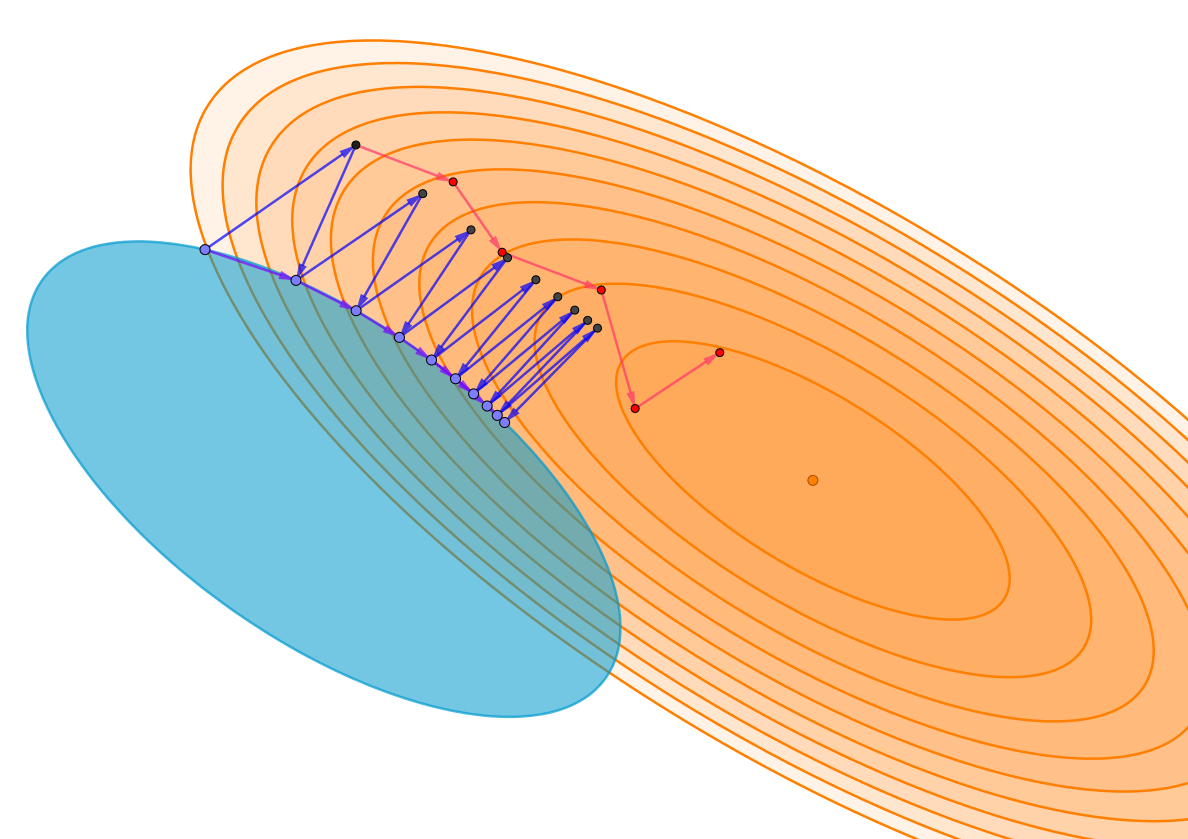
\includegraphics[width=0.75\textwidth]{./images/gradient.png}
    \caption{Las áreas naranjas sombreadas representan curvas de nivel de la función $f(x,y) = 2(x+y)^2 + 2y^2$ para valores naturales entre $0$ y $10$. El camino rojo muestra el comportamiento del gradiente descendente sin restricciones aplicado a la función $f$. El camino azul muestra el funcionamiento del gradiente con proyecciones sobre la elipse azul.} \label{fig:gradient}
\end{figure}

\subsection{Método de las proyecciones iteradas}

Si trabajamos con problemas convexos con restricciones, podemos encontrarnos con más de una restricción, de forma que no conozcamos una proyección explícita sobre el conjunto viable, que es la intersección de los conjuntos asociados a cada restricción. Un método que permite calcular un punto en dicha intersección, si conocemos las proyecciones sobre cada uno de los conjuntos que definen las restricciones, es el conocido como \emph{método de las proyecciones iteradas}, que consiste en ir proyectando el punto sucesivas veces en cada uno de los conjuntos asociados a cada restricción. Dicha sucesión de proyecciones converge a la intersección, por lo que este método iterativo puede utilizarse para forzar la satisfacción de las restricciones en un problema convexo. Veamos que efectivamente el método de las proyecciones iteradas converge. Lo vamos a ver para dos restricciones. El caso general se prueba siguiendo el mismo razonamiento.

\begin{thm}[Convergencia de las proyecciones iteradas] \label{thm:iter_proj}
    Sean $C, D \subset \R^d$ conjuntos convexos cerrados y sean $P_C, P_D \colon R^d \to R^d$ las proyecciones sobre $C$ y $D$, respectivamente. Supongamos que $x_0 \in C$ y construimos las sucesiones $\{x_n\}$ e $\{y_n\}$ dadas por $y_n = P_D(x_n)$ y $x_{n+1} = P_C(y_n)$, para cada $n \in \mathbb{N}$.

    Entonces, si $C \cap D \ne \emptyset$, ambas sucesiones convergen a un punto $x^* \in C \cap D$.
\end{thm}

\begin{proof}
    Fijamos $\overline{x} \in C\cap D$ arbitrario. Si existe algún $k \in \N$ tal que $x_k \in C\cap D$ o $y_k \in C\cap D$, entonces $x_n = y_n = x_k \in C \cap D$, para todo $n > k$, lo que finalizaría la prueba. Por tanto, a partir de ahora supondremos que $x_n,y_n \notin C \cap D$ para todo $n \in \N$.

    Observemos que, como $y_n = P_D(x_n)$ para todo $n \in \N$, el teorema de la proyección convexa \ref{thm:convex_projection} nos dice que el semiespacio $\{ z \in \R^d \colon \langle x_n - y_n, z - y_n \rangle \le 0 \}$ contiene a $D$. Aplicando esto a $\overline{x} \in C\cap D \subset D$, se tiene que
    \begin{equation*}
        \begin{split}
            \|x_n - \overline{x}\|^2 &= \|x_n - y_n + y_n - \overline{x}\|^2 \\
                                     &= \|x_n - y_n\|^2 + \|y_n - \overline{x}\|^2 + 2 \langle x_n - y_n, y_n - \overline{x}\rangle \\
                                     &= \|x_n - y_n\|^2 + \|y_n - \overline{x}\|^2 - 2 \langle x_n - y_n, \overline{x} - y_n\rangle \\
                                     &\ge \|x_n - y_n\|^2 + \|y_n - \overline{x}\|^2. 
        \end{split}
    \end{equation*}
    Por tanto,
    \begin{equation} \label{eq:iter_proj_proof:1}
        \|y_n - \overline{x}\|^2 \le \|x_n - \overline{x}\|^2 - \|y_n - x_n\|^2 \le \|x_n - \overline{x}\|^2 \quad \forall n \in \N.
    \end{equation}
    Análogamente, como $x_{n+1} = P_C(y_n)$, se tiene que el semiespacio $\{ z \in \R^d \colon \langle y_n - x_{n+1}, z - x_{n+1} \rangle \le 0\}$ contiene a $C$, y razonando como en la expresión anterior se deduce que
    \begin{equation} \label{eq:iter_proj_proof:2}
        \|x_{n+1} - \overline{x}\|^2 \le \|y_n - \overline{x}\|^2 - \|x_{n+1} - y_n\|^2 \le \|y_n - \overline{x}\|^2 \quad \forall n \in \N.
    \end{equation}
    En particular, se tiene que $\|x_n - \overline{x}\| \le \|x_0 - \overline{x}\|$ y $\|y_n - \overline{x}\| \le \|x_0 - \overline{x}\|$, para cada $n \in \N$, y en consecuencia $\{x_n\}$ e $\{y_n\}$ están acotadas. Por tanto, $\{x_n\}$ admite una parcial convergente a un punto $x^* \in C$, por ser $C$ cerrado y $\{x_n\} \subset C$. Veamos que también $x^* \in D$, y que es el límite de las sucesiones $\{x_n\}$ e $\{y_n\}$.

    De las expresiones \ref{eq:iter_proj_proof:1} y \ref{eq:iter_proj_proof:2} se deduce que la sucesión $\{\|z_n - \overline{x}\|\}$, donde $z_{2k} = x_k$ y $z_{2k+1} = y_k$, para $k \in \N \cup\{0\}$, es decreciente. Como además está minorada, converge. Las sucesiones $\{\|x_n - \overline{x}\|\}$ e $\{\|y_n - \overline{x}\|\}$ son parciales de la sucesión anterior, luego convergen al mismo límite, que llamaremos $L$. Si tomamos límites superiores en \ref{eq:iter_proj_proof:1}, obtenemos que $L^2 \le L^2 - \limsup\{\|y_n - x_n\|^2\} \le L^2$, luego $\limsup\{\|y_n - x_n\|^2\} = 0$. Análogamente, tomando límites inferiores, se deduce que $\liminf\{\|y_n - x_n\|^2\} = 0$, luego $\|y_n - x_n \| \to 0$. Razonando igualmente con la expresión \ref{eq:iter_proj_proof:2}, se obtiene que también $\|x_{n+1} - y_n\| \to 0$. Como $d(x_n,D) = d(x_n,P_D(x_n)) = d(x_n,y_n) = \|x_n - y_n \| \to 0$ y $x^*$ es el límite de una sucesión parcial de $\{x_n\}$, se deduce que $d(x^*,D) = 0$, y como $D$ es cerrado, se tiene $x^* \in D$, luego $x^* \in C\cap D$.

    Como $\overline{x}$ era arbitrario, podemos tomar $\overline{x} = x^* \in C\cap D$. Entonces, por lo ya visto para $\overline{x}$, se tiene que las sucesiones $\{\|x_n - x^*\|\}$ e $\{\|y_n - x^*\|\}$ son decrecientes, luego convergen. Como $x^*$ era el límite de una parcial de $\{x_n\}$, se deduce que $\{\|x_n - x^*\|\} \to 0$. Finalmente, $\|y_n - x^*\| \le \|y_n - x_n\| + \|x_n - x^*\| \to 0$, concluyendo así con la convergencia de las proyecciones iteradas.

\end{proof}

Para concluir, es interesante destacar que el teorema anterior admite una versión cuando la intersección es vacía. En tal caso, es posible probar que, si hay puntos donde se alcanza la distancia entre los conjuntos $C$ y $D$, las sucesiones convergerán, cada una en su conjunto, a uno de esos puntos \cite{proximity_convex}. También, notemos que, cuando $C \cap D \ne \emptyset$, el límite de las sucesiones no es necesariamente la proyección sobre la intersección. Sin embargo, un razonamiento mediante hiperplanos soporte similar al utilizado en el método del gradiente con proyecciones permite ver que la dirección que apunta al límite es también una dirección de descenso. En la figura \ref{fig:iterproj} se muestra gráficamente el funcionamiento del método de las proyecciones iteradas en ambos casos.

\begin{figure}[h]
    \centering
    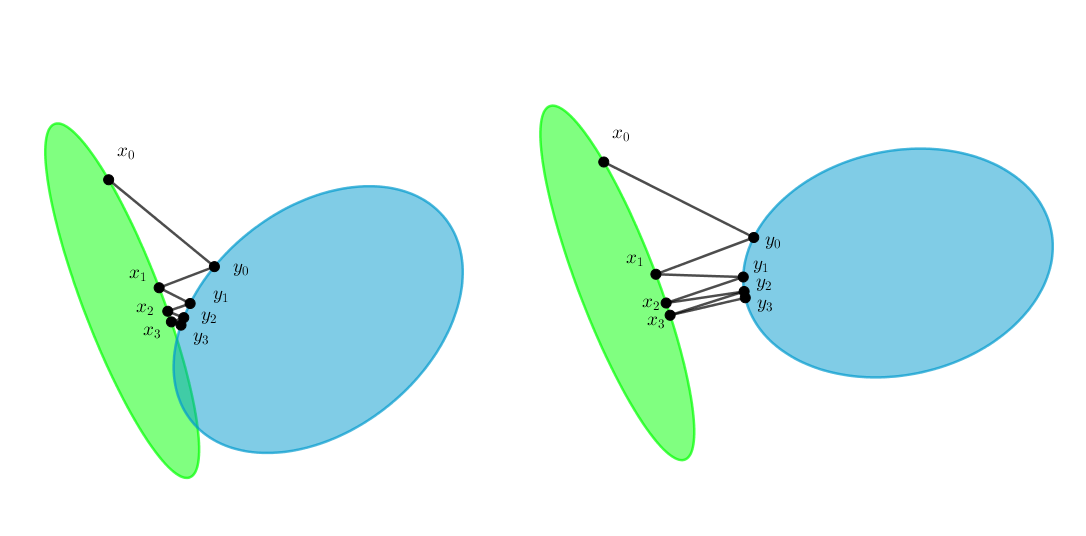
\includegraphics[width=0.75\textwidth]{./images/iterated_projections.png}
    \caption{Método de las proyecciones iteradas. La segunda imagen muestra el desarrollo del método cuando los conjuntos no se cortan.} \label{fig:iterproj}
\end{figure}

\subsection{Subgradientes}

Recordemos que cuando $f \colon \Omega \to \R$, con $\Omega$ convexo y abierto, es convexa y diferenciable, se verifica que $f(x) \ge \langle \nabla f(x_0), x - x_0 \rangle$ para cualesquiera $x,x_0 \in \Omega$. En general, si $f\colon A \to \R$ es una función arbitraria, cualquier vector $v \in \R^d$ que verifique, para $x_0 \in A$, que $f(x) \ge f(x_0)+ \langle v, x - x_0 \rangle$ para todo $x \in A$ se denomina un \emph{subgradiente} de $f$ en $x_0$. Una función puede no tener, o tener más de un subgradiente. El conjunto de los subgradientes se $f$ en el punto $x_0$ se denotará por $\partial f(x_0)$ (o $\partial f(x_0)/\partial x$, si es necesario especificar la variable).

El subgradiente tiene un comportamiento similar al del gradiente, y por ello se utilizan como método de descenso cuando la función no es diferenciable. Es importante notar que no todos los subgradientes llevan siempre una dirección de descenso, ni necesariamente han de existir. En el caso de las funciones convexas sí que podemos garantizar la existencia de subgradientes en todos los puntos.

\begin{prop}
    Sea $\Omega \subset \R^d$ un abierto convexo. Una función $f \colon \Omega \to \R$ es convexa si y solo si admite subgradientes en todo punto de $\Omega$.
\end{prop}

\begin{proof}
    Por un lado, $f$ es convexa si y solo si $\epi(f)$ es convexo. Por ser $\Omega$ abierto, $\epi(f)$ tiene interior no vacío en $\R^{d+1}$. Por otro lado, $v$ es un subgradiente de $f$ en $x_0$ si y solo si $(v,-1)$ define un hiperplano soporte en $\epi(f)$ sobre el punto frontera $(x_0,f(x_0))$. Esto se debe a que $(x,t) \in \epi(f)$, si y solo si $t \ge f(x) \ge f(x_0) + \langle v, x - x_0 \rangle$, lo cual ocurre si y solo si $\langle v,x \rangle - t \le f(x_0) + \langle v, x_0 \rangle \iff \langle (v,-1),(x,t) \rangle f(x_0) + \langle v,x_0 \rangle$. Gracias a estas caracterizaciones, el teorema del hiperplano soporte \ref{thm:support_hyperplane} garantiza el resultado buscado.
\end{proof}

Por tanto, sobre funciones convexas podemos tomar subgradientes en todo punto e iterar de forma análoga al gradiente descendente o al gradiente con proyecciones. Como ya se ha dicho, el subgradiente puede no llevar una dirección de descenso. Por ello, al aplicar este método se suele almacenar el mejor valor obtenido. Aunque exista más de un subgradiente, solo necesitamos calcular uno para aplicar el método del subgradiente. En los algoritmos que trataremos el cálculo de subgradientes será sencillo. Por ejemplo, si $f$ es diferenciable en $x$, podemos tomar el subgradiente $\nabla f(x)$ (de hecho, este es el único subgradiente en este caso). El otro caso de interés que trataremos será el cálculo del subgradiente de máximos de funciones convexas diferenciables.

\begin{prop}
    Sea $\Omega \subset \R^d$ abierto y convexo, y $f_i\colon \Omega \to \R$, con $i\in \{1,\dots,r\}$, funciones convexas diferenciables. Sea $f \colon \Omega \to \R$ definida fomo $f(x) = \max_i f_i(x)$. Dado $x \Omega$, tomamos $j \in \{1,\dots,r\}$ tal que $f(x) = f_j(x)$. Entonces, $\nabla f_j(x) \in \partial f(x)$.
\end{prop}

\begin{proof}
    Como $f_j$ es convexa se tiene que, para todo $y \in \Omega$, $f_j(y) \ge f_j(x) + \langle y-x, \nabla f_j(x) \rangle$. Como $f(x) = f_j(x)$ y $f(y) \ge f_j(y)$, se concluye que
    \[ f(y) \ge f(x) + \langle y-x, \nabla f_j(x) \rangle. \]
\end{proof}


%% CAPÍTULO 2 - MATRICES
\chapter{Análisis matricial} \label{chapter:matrices}

En el aprendizaje de métricas de distancia, las matrices tendrán un papel fundamental, pues serán la estructura que definirá las distancias y sobre la que se aplicarán los métodos de optimización estudiados en el capítulo anterior. Dentro del conjunto de todas las matrices, las matrices semidefinidas serán de aún mayor importancia, por lo que para comprender mejor los problemas de aprendizaje con los que trataremos será necesario profundizar en algunas de sus numerosas propiedades.

Este capítulo profundiza en el estudio de las matrices, partiendo de los resultados más conocidos de diagonalización en el álgebra lineal. Desde esta base, se introducirá un producto escalar en el espacio de las matrices, convirtiéndolas así en un espacio de Hilbert, añadiendo de esta forma propiedades métricas y topológicas que analizaremos. A continuación nos centraremos en las matrices definidas positivas, estudiando varios teoremas de descomposición que serán de gran utilidad. También veremos cómo el producto escalar que hemos añadido permite demostrar un teorema de proyección que motivará muchos de los algoritmos que se estudiarán más adelante. Por último, analizaremos cómo trabajar con problemas de optimización basados en matrices, haciendo especial hincapié en determinados problemas de optimización que se pueden resolver mediante vectores propios.

\section{Preliminares}

Nos centraremos en el estudio de las matrices con entradas reales, pues el problema que vamos a tratar será en variable real, si bien muchos de los resultados que vamos a ver son extensibles al caso complejo. Introducimos en primer lugar la notación que utilizaremos para las matrices a lo largo de este trabajo.

Notaremos el espacio de las matrices reales de dimensión $d' \times d$ como $\mathcal{M}_{d'\times d}(\R)$. Cuando $d' = d$, entonces abreviaremos, notando el espacio de las matrices cuadradas de orden $d$ como $\mathcal{M}_d(\R)$. Una matriz $A \in \mathcal{M}_{d'\times d}(\R)$ también la podremos expresar, aludiendo a sus entradas, como $A = (A_{ij})_{\substack{i=1,\dots,d' \\ j=1,\dots,d}}$, donde $A_{ij} \in \R$ representa la entrada en la fila $i$-ésima y columna $j$-ésima. También usaremos la notación $A_{.j}$ para aludir a la columna $j$-ésima completa de la matriz, vista como vector, y análogamente $A_{i.}$ para la fila $i$-ésima. Los vectores $v = (v_1,\dots,v_d) \in \R^d$ los trataremos como matrices columna.

Dada $A = (A_{ij}) \in \mathcal{M}_{d'\times d}(\R)$, notaremos la matriz traspuesta de $A$ como $A^T = (A_{ji}) \in \mathcal{d\times d'}(\R)$. El conjunto de las matrices simétricas de orden $d$ lo notaremos por $S_d(\R) = \{ A \in \mathcal{M}_d(\R) \colon A = A^T\}$. Al conjunto de las matrices antisimétricas lo expresaremos como $A_d(\R) = \{A \in \mathcal{M}_d(\R) \colon A = -A^T$. El conjunto de las matrices regulares de orden $d$ o grupo lineal de orden $d$ lo escribiremos como
\begin{align*}
\gl_d(\R) &= \{A \in \mathcal{M}_d(\R) \colon \exists A^{-1} \in \mathcal{M}_d(\R) \colon AA^{-1} = A^{-1}A = I \}\\
          &= \{A \in \mathcal{M}_d(\R) \colon \det(A) \ne 0\} = \{A \in \mathcal{M}_d(\R) \colon r(A) = d\},
\end{align*}
donde las operaciones $r$ y $\det$ hacen referencia al rango y al determinante, respectivamente. También utilizaremos el operador traza, que notaremos por $\tr$. Una matriz $A \in \mathcal{M}_{d}(\R)$ diremos que es ortogonal si es regular y $A^T = A^{-1}$. El conjunto de las matrices ortogonales lo notaremos por $O_d(\R)$.

Una matriz $M \in S_d(\R)$ diremos que es semidefinida positiva si se verifica que $x^T M x \ge 0$ para todo $x \in \R^d$. Si además se tiene que $x^TMx = 0 \iff x = 0$, diremos que $M$ es definida positiva. Notaremos a estos conjuntos por $\mathcal{M}_d(\R)^+_0$ y $\mathcal{M}_d(\R)^+$, respectivamente. Las matrices semidefinidas positivas (resp. definidas positivas) se caracterizan por tener todos sus valores propios no negativos (resp. positivos). Análogamente se definen las matrices semidefinidas y definidas negativas, y se notan por $\mathcal{M}_d(\R)^-_0$ y $\mathcal{M}_d(\R)^-$.

Es conocido que, fijada una base en $\R^d$, las matrices de dimensión $d' \times d$ se identifican con el conjunto de aplicaciones lineales de $\R^d$ en $\R^{d'}$ de forma biunívoca. Por tanto, si es necesario, una matriz $L \in \mathcal{M}_{d'\times d}(\R)$ la veremos como una aplicación lineal $L \colon \R^d \to \R^{d'}$, notando ambas de la misma forma. También es conocido que las matrices simétricas se identifican con operadores autoadjuntos si la base fijada es ortonormal. Pero las matrices simétricas $A \in S_d(\R)$ además pueden identificarse con formas bilineales simétricas, esto es, aplicaciones de la forma $g_A \colon \R^d \to \R^d$ dadas por $g_A(x,y) = x^TAy$, que además son semidefinidas o definidas positivas si la matriz $A$ lo es. De nuevo, según las circunstancias, podremos ver las matrices simétricas como aplicaciones, si es necesario.

\section{Las matrices como espacio de Hilbert}

Sobre el conjunto de las matrices de determinada dimensión tenemos definida una operación de suma, y además tenemos definido un producto entre matrices de órdenes $d \times r$ y $r \times n$, que cuando nos restringimos a matrices cuadradas, se convierte en un producto interno, que junto con la suma da al espacio vectorial de las matrices una estructura de anillo no conmutativo. Con estas operaciones solo podemos obtener propiedades algebraicas sobre las matrices. Si queremos desarrollar una teoría geométrica sobre ellas tendremos que introducir una topología adecuada. La topología que introduciremos permitirá tratar el espacio de matrices $\mathcal{M}_{d'\times d}(\R)$ como un espacio de Hilbert idéntico a $\R^{d'\times d}$. Esta identificación será únicamente a nivel de espacios de Hilbert, de forma que con las herramientas matriciales como el producto matricial o los valores propios podremos estudiar propiedades que en general no se presentan en $\R^{d'\times d}$ como espacio vectorial.

\begin{definition}
    Se define el \emph{producto escalar de Frobenius} en el espacio de matrices de orden $d' \times d$ como la aplicación $\langle \cdot, \cdot \rangle_F \colon \mathcal{M}_{d' \times d}(\R) \times \mathcal{M}_{d' \times d}(\R) \to \R$ dada por
    \[ \langle A, B \rangle_F = \sum_{i=1}^d\sum_{j=1}^{d'} A_{ij}B_{ij} = \tr(A^TB). \]
    Se define la \emph{norma de Frobenius} en el espacio de matrices de orden $d' \times d$ como la aplicación $\|\cdot \|_F \colon \mathcal{M}_{d' \times d}(\R) \to \R^+_0$ dada por
    \[ \|A\|_F = \sqrt{\langle A^T, A \rangle} = \sqrt{\sum_{i=1}^d\sum_{j=1}^{d'}A_{ij}^2} = \sqrt{\tr(A^TA)} \]
\end{definition}

Se tiene que $(\mathcal{M}_{d'\times d}(\R),\langle \cdot, \cdot \rangle_F)$ es un espacio de Hilbert, y su producto escalar es el mismo que si calculáramos el producto escalar usual de la matriz vista como vector en $\R^{d' \times d}$, añadiendo las filas al vector una detrás de otra.

La norma de Frobenius es, por tanto, idéntica a la norma euclidea en $\mathbb{R}^{d'\times d}$ realizando la misma identificación entre matrices y vectores. Vista como norma matricial, verifica propiedades adicionales. Por ejemplo, si consideramos matrices cuadradas, tenemos que la norma de Frobenius es submultiplicativa, esto es, $\|AB\|_F \le \|A\|_F\|B\|_F$, para $A, B \in \mathcal{M}_d(\R)$. Esto se deduce aplicando las definiciones de norma de Frobenius y producto matricial, y aplicando la desigualdad de Cauchy-Schwarz para el producto escalar en $\R^d$. De hecho, la desigualdad se verifica para matrices no cuadradas, siempre que las dimensiones permitan multiplicarlas, y tomando en cada caso la norma de Frobenius en el espacio adecuado.

Muchas de las normas que se definen para las matrices cuadradas tienen la propiedad de que son \emph{inducidas} por una norma vectorial, esto es, la norma $\matrixnorm{\cdot}$ en $\mathcal{M}_{d}(\R)$ está inducida por la norma $\|\cdot\|$ en $\R^{d}$ si para toda $A \in \mathcal{M}_{d}(\R)$ se tiene
\[ \matrixnorm{A} = \sup \{ \|Ax\| \colon x \in \R^d, \|x\| = 1 \} = \sup\left\{ \frac{\|Ax\|}{\|x\|} \colon x \in \R^d \setminus \{0\} \right\}. \]
En este caso, se tiene que la norma de Frobenius no está inducida por ninguna norma vectorial, para $d \ge 2$. Observemos que todas las normas inducidas por una norma vectorial han de verificar $\matrixnorm{I} = 1$, lo cual no ocurre con la norma de Frobenius, pues $\|I\|_F = \sqrt{d} > 1$.

Además de las ya comentadas, es importante destacar las siguientes propiedades de la norma de Frobenius.

\begin{prop}~ \label{prop:prop_frobenius}
    \begin{enumerate}
        \item Para cada $A \in \mathcal{M}_{d' \times d}(\R)$, $\|A\|_F = \|A^T\|_F$.
        \item Para cada $A \in \mathcal{M}_{d' \times d}(\R)$, $\|A\|_F = \sqrt{\tr(AA^T)}$
        \item Si $U \in O_d(\R), V \in O_{d'}(\R)$ y $A \in \mathcal{M}_{d' \times d}(\R)$, entonces $\|AU\|_F = \|VA\|_F = \|VAU\|_F = \|A\|_F$.
        \item Si $A \in S_d(\R)$, entonces $\|A\|_F^2 = \sum_{i=1}^d \lambda_i^2$, donde $\lambda_1,\dots,\lambda_d$ son los valores propios de $A$.
        \item Si $A \in S_d(\R)$, entonces, $\rho(A) \le \|A\|_F \le \sqrt{d}\rho(A)$, donde $\rho(A) = \max\{|\lambda| \colon \lambda \in \R \text{ es valor propio de } A\}$ es el \emph{radio espectral} de $A$.
        %\item Si $d' \le d$, para cada $A \in \mathcal_{d' \times d}(\R)$, $\|A\|_F^2 = \sum_{i=1}^{d'} \sigma_i^2$, donde $\sigma_1, \dots, \sigma_{d'}$ son los valores propios de $AA^T$ (que coinciden con los de $A^TA$, teniendo este último $d - d'$ valores propios adicionales con valor $0$).
    \end{enumerate}
\end{prop}

\begin{proof}~
    \begin{enumerate}
        \item Es evidente.
        \item Consecuencia de la invarianza de la traza por permutaciones cíclicas.
        \item Se tiene
            \begin{align*}
                \|AU\|_F^2 &= \tr((AU)^T(AU)) = \tr(U^TA^TAU) = \tr(UU^TA^TA) = \tr(A^TA) = \|A\|^2_F \\
                \|VA\|_F^2 &= \tr((VA)^T(VA)) = \tr(A^TV^TVA) = \tr(A^TA) = \|A\|_F^2 
            \end{align*}
        \item Si $A \in S_d(\R)$, existe una matrix $U \in O_d(\R)$ tal que $A = UDU^T$ y $D = \diag(\lambda_1,\dots,\lambda_d)$ es la matriz diagonal con los valores propios de $A$. Entonces, por la propiedad anterior,
        \[ \|A\|_F^2 = \|UDU^T\|_F^2 = \|D\|_F^2 = \sum_{i,j=1}^d D_{ij}^2 = \sum_{i=1}^d \lambda_i^2. \]
        \item Si $D = \diag(\lambda_1,\dots,\lambda_d)$ es la matriz diagonal con los valores propios de $A$, se tiene que
        \[ \rho(A) = \|(\lambda_1,\dots,\lambda_d)\|_{\infty} \le \|(\lambda_1,\dots,\lambda_d)\|_2 \le \sqrt{d}\|(\lambda_1,\dots,\lambda_d)\|_{\infty} = \sqrt{d}\rho(A). \]
        El resultado se tiene al observar que $\|(\lambda_1,\dots,\lambda_d)\|_2 = \|D\|_F = \|A\|_F$.
        %\item Tiene pinta de que hace falta SVD y tampoco la vamos a usar, creo


    \end{enumerate}

\end{proof}

Para concluir, observemos que, teniendo las matrices identificadas como elementos de un espacio vectorial de dimensión finita con producto escalar, todas las teorías métricas pueden ser desarrolladas de la misma forma que las teorías en un espacio $\R^d$. En particular, todos los resultados vistos en el capítulo anterior pueden aplicarse sobre las matrices.

\begin{comment}
Para concluir la sección, es interesante destacar algunas propiedades topológicas de las que disponen algunos de los subconjuntos más destacados de matrices con el producto escalar que hemos añadido.

\begin{prop}~
    En las siguientes propiedades suponemos fijada una dimensión $d' \times d$ (con $d' = d$ cuando la propiedad esté definida solo en espacios de matrices cuadradas).
    \begin{enumerate}
        \item Las aplicaciones traza y determinante son continuas.
        \item La suma, el producto y la trasposición de matrices son continuos.
        \item El conjunto de todas las matrices es un espacio vectorial. Las matrices simétricas (resp. antisimétricas) forman un subespacio vectorial del espacio de matrices cuadradas. En consecuencia, son convexos y por tanto conexos.
        \item El conjunto de las matrices regulares (o isomorfismos vectoriales) es abierto y tiene dos componentes conexas: los isomorfismos que preservan la orientación (determinante positivo) y los que la invierten (determinante negativo).
        \item El grupo ortogonal (o grupo de isometrías) tiene también dos componentes conexas: las isometrías que preservan la orientación, y las que la invierten. Además, es compacto.
    \end{enumerate}
\end{prop}

\begin{proof}~
    \begin{enumerate}
        \item Ambas aplicaciones son polinomios en las entradas de la matriz.
        \item Cada componente de las funciones es un polinomio en las entradas de las matrices que reciben como argumento.
        \item La comprobación de que son espacios vectoriales es inmediata. Son convexos por serlo todos los subespacios vectoriales.
    \end{enumerate}
\end{proof}
\end{comment}

\section{Matrices semidefinidas positivas: teoremas de descomposición y proyección}

\subsection{El cono de las matrices semidefinidas positivas}

En esta sección nos centraremos en el estudio de las matrices semidefinidas positivas. Comenzaremos viendo su estructura algebraica como conjunto. Sean $A, B \in \mathcal{M}_d(\R)^+_0$ y $\alpha_1, \alpha_2 \in \R^+_0$. Entonces, dado $x \in \R^d$,
\[ x^T(\alpha_1A + \alpha_2B)x = \alpha_1(x^TAx) + \alpha_2(x^TBx) \ge 0, \]
luego $\alpha_1A + \alpha_2B \in \mathcal{M}_d(\R)^+_0$. Por tanto, el conjunto de las matrices semidefinidas positivas tiene estructura de cono, y en particular es convexo. Viendo este conjunto como subconjunto de las matrices simétricas, y con la topología inducida por estas, tenemos que el cono de matrices semidefinidas positivas verifica también las siguientes propiedades:
\begin{itemize}
    \item Es cerrado. Podemos ver
    \[\mathcal{M}_d(\R)^+_0 = \{ M \in S_d(\R) \colon x^TMx \ge 0 \quad \forall x \in \R^d \} = \bigcap_{x \in \R^d} \{ M \in S_d(\R) \colon x^T M x \ge 0 \}. \]
    Los elementos en la intersección son semiespacios cerrados, dentro del conjunto de las matrices simétricas, pues la aplicación $M \mapsto x^TMx$ es lineal en $M$, fijado $x \in \R^d$. Por tanto, la intersección es cerrada.
    \item Es puntiagudo. Observemos que $-\mathcal{M}_d(\R)^+_0 = \mathcal{M}_d(\R)^-_0$. Si $M \in \mathcal{M}_d(\R)^+_0 \cap \mathcal{M}_d(\R)^-_0$, entonces se tiene que todos sus valores propios son no negativos y no positivos, luego todos sus valores propios son $0$, y esto solo es posible si $M = 0$.

    \item Es sólido. Concretamente, su interior es $\mathcal{M}_d(\R)^+$, que es no vacío. Para probarlo utilizaremos el siguiente resultado.
\end{itemize}

\begin{prop}[Propiedades de regularización]~ \label{prop:pd_regularization}
    \begin{enumerate}
        \item Sea $M \in S_d(\R)$. Entonces, existe $\varepsilon > 0$ tal que $M + \varepsilon I \in \mathcal{M}_d(\R)^+$.
        \item Sea $M \in \mathcal{M}_d(\R)^+_0$. Entonces, para todo $\varepsilon > 0$, se tiene que $M + \varepsilon I \in \mathcal{M}_d(\R)^+$.
    \end{enumerate}
\end{prop}

\begin{proof}
    Sea $M \in S_d(\R)$. Entonces, todos sus valores propios son reales, y son raíces del polinomio característico $p(\lambda) = \det(M - \lambda I)$. Si llamamos $\lambda_1 \le \dots \le \lambda_d$ a los valores propios de $M$, para cada $\varepsilon \in \R$ se tiene que las raíces del polinomio $q(\lambda) = p(\lambda - \varepsilon)$ son $\lambda_1 + \varepsilon \le \dots \le \lambda_d + \varepsilon$. Además, el polinomio $q$ es justo el polinomio característico asociado a $M + \varepsilon I$, pues $\det( (M + \varepsilon - I) - \lambda I) = \det(M - (\lambda - \varepsilon)I ) = p(\lambda  \varepsilon) = q(\lambda)$.

    Por tanto, si tomamos $\varepsilon > \max\{-\lambda_1, 0\} \ge 0$, todos los valores propios de $M + \varepsilon I$ serán positivos, y por tanto $M + \varepsilon I \in \mathcal{M}_d(\R)^+$. Si se tenía $M \in \mathcal{M}_d(\R)^+_0$, entonces conseguimos que los valores propios sean positivos para cualquier $\varepsilon > 0$.
\end{proof}

La propiedad anterior es muy interesante desde el punto de vista computacional, pues en ocasiones los errores de precisión en los cálculos con matrices hacen que se pierda la condición de ser definida positiva. El resultado anterior nos dice que podemos recuperarla añadiendo un valor positivo a la diagonal de la matriz, siendo tan pequeño como queramos en el caso de tener una matriz semidefinida. De aquí que se enuncien como propiedades de regularización. Con estas propiedades vamos a terminar de ver que el interior del conjunto de matrices semidefinidas positivas son las matrices definidas positivas (viéndolas dentro de las matrices simétricas).

\begin{cor}
    $\mathcal{M}_d(\R)^+_0$ es un cono propio con interior $\mathcal{M}_d(\R)^+$.
\end{cor}
\begin{proof}
    Ya hemos visto que $\mathcal{M}_d(\R)^+_0$ es un cono cerrado y puntiagudo. Queda comprobar que su interior es el conjunto de las matrices definidas positivas. Notamos a las bolas inducidas por la norma de Frobenius sobre las matrices simétricas como $B(M,r) = \{ A \in S_d(\R) \colon \|M - A\|_F < r\}$, para cada $M \in S_d(\R)$ y $r > 0$.

    Veamos que $\interior{(\mathcal{M}_d(\R)^+_0)} \subset \mathcal{M}_d(\R)^+$. Sea $M \in \interior{(\mathcal{M}_d(\R)^+_0)}$. Entonces, existe $\varepsilon > 0$ tal que $B(M,2\varepsilon\sqrt{d}) \subset \mathcal{M}_d(\R)^+_0$. Sea $A = M - \varepsilon I$. Se tiene que $\|M - A\|_F = \|\varepsilon I\|_F = \varepsilon\sqrt{d}$, luego $A \in B(M,2\varepsilon\sqrt{d}) \subset \mathcal{M}_d(\R)^+_0$. Por la proposición anterior, $M = A + \varepsilon I \in \mathcal{M}_d(\R)^+$.

    Veamos que $\mathcal{M}_d(\R)^+$ es abierto. El criterio de Sylvester nos dice que $M \in \mathcal{M}_d(\R)^+$ si y solo si todos sus menores principales son positivos, esto es, si y solo si $\det(M_k) > 0$ para cada $k \in \{1,\dots,d\}$, donde $M_k \in \mathcal{M}_k(\R)$ es la matriz de orden $k$ cuyas entradas coinciden con las de $M$ hasta dicha dimensión. En consecuencia,
    \[\mathcal{M}_d(\R)^+ = \{M \in S_d(\R) \colon \det(M_k) > 0 \quad \forall k = 1,\dots,d \} = \bigcap_{k=1}^d\{M \in \mathcal{S}_d(\R) \colon \det(M_k) > 0 \}. \]
    Por la continuidad del determinante, tenemos una intersección finita de conjuntos abiertos en $S_d(\R)$ (son abiertos en $\mathcal{M}_d(\R)$, intersecados con $S_d(\R)$). Por tanto, $\mathcal{M}_d(\R)^+$ es abierto.

    Como $\mathcal{M}_d(\R)^+ \subset \mathcal{M}_d(\R)^+_0$ y $\mathcal{M}_d(\R)^+$ es abierto, tomando interiores se deduce la inclusión restante.
\end{proof}

Puesto que hemos probado que las matrices semidefinidas positivas son un cono propio sobre las matrices simétricas, tenemos definidas sobre estas la relación de orden $\preceq$, dada por $A \preceq B \iff B - A \in \mathcal{M}_d(\R)^+_0$. Análogamente, tenemos el orden estricto dado por $A \prec B \iff B - A \in \mathcal{M}_d(\R)^+$. Estos órdenes se denominan órdenes de \emph{Löwner} Veamos algunas de sus principales propiedades.

\begin{prop}[Propiedades del orden de las matrices semidefinidas]~
    Supongamos $A,B,M \in S_d(\R)$.
    \begin{enumerate}
        \item $M \in \mathcal{M}_d(\R)^+_0 \iff M \succeq 0$ y $M \in \mathcal{M}_d(\R)^+ \iff M \succ 0$.
        \item $A \preceq B \iff x^TAx \le x^TBx$ para todo $x \in \R^d$.
        \item $A \prec B \iff x^TAx < x^TBx$ para todo $x \in \R^d\setminus\{0\}$.
        \item Si $A \preceq B$, entonces $C^TAC \preceq C^TBC$, para todo $C \in \mathcal{M}_d(\R)$.
        \item Si $A \prec B$, entonces $C^TAC \prec C^TBC$ para todo $C \in \gl_d(\R)$.

    \end{enumerate}
\end{prop}

\begin{proof}~
    \begin{enumerate}
        \item Es evidente.
        \item $A \preceq B \iff B - A \succeq 0 \iff x^T(B-A)x \ge 0$ para todo $x \in \R^d$ $\iff x^TBx \ge x^TAx$ para todo $x \in \R^d$.
        \item La prueba es análoga a la anterior.
        \item Basta ver que $B - A \succeq 0 \implies C^T(B-A)C \succeq 0$:
            \[B - A \succeq 0 \implies (Cx)^T(B-A)(Cx) \ge 0 \quad \forall x \in \R^d \implies x^T(C^T(B-A)C)x \ge 0 \quad \forall x \in \R^d \implies C^T(B-A)C \succeq 0. \]
        \item La prueba es análoga a la anterior, teniendo en cuenta que $Cx \ne 0$ para todo $x \ne 0$, pues $C$ es regular.
    \end{enumerate}
\end{proof}

\subsection{Teoremas de descomposición}

Los próximos resultados que veremos serán teoremas de descomposición para matrices semidefinidas positivas, o basadas en estas. Estos resultados nos permitirán, por un lado, proporcionar varias alternativas para parametrizar el problema que trataremos en el capítulo \ref{chapter:dml_theory}. Por otra parte, estos teoremas de descomposición proporcionan la base para muchos algoritmos de factorización de matrices, como es el caso de la factorización de Cholesky, o la descomposición en valores singulares. Por último, estos resultados nos mostrarán que el cono de las matrices semidefinidas positivas permite generalizar algunos conceptos adicionales definidos para los números no negativos, como es el caso de las raíces cuadradas o el valor absoluto, manteniendo algunas de sus propiedades.

Comenzaremos con una caracterización de las matrices semidefinidas positivas por descomposición, la cual nos permitirá introducir además el concepto de raíz cuadrada. Utilizaremos para ello un lema previo.

\begin{lem} \label{lem:poly_conmute}
    Sean $A, B \in \mathcal{M}_d(\R)$ dos matrices que conmutan, es decir, $AB = BA$. Entonces, $Ap(B) = p(B)A$, donde $p$ denota cualquier polinomio sobre matrices (es decir, una expresión de la forma $p(C) = a_0I + a_1C + a_2C^2 + \dots a_nC^n$, con $a_1,\dots,a_n \in \R$).
\end{lem}
\begin{proof}
    Basta ver que
    \[AB^n = (AB)B^{n-1} = B(AB)B^{n-2} = \dots = B^{n-1}(AB) = B^nA, \]
    y $Ap(B) = p(B)A$ se deduce por linealidad.
\end{proof}

\begin{lem} \label{lem:poly_diag_sqrt}
    Sea $D \in \mathcal{M}_d(\R)^+_0$ una matriz diagonal. Entonces, existe un polinomio sobre matrices $p$ tal que $p(D^2) = D$.
\end{lem}
\begin{proof}
    Supongamos $D = \diag(\lambda_1,\dots,\lambda_d)$, con $0 \le \lambda_1 \le \dots \lambda_d$. Entonces, $D^2 = \diag(\lambda_1^2,\dots\lambda_d^2)$. Tomamos un polinomio $p$ de interpolación en los puntos $(\lambda_i^2,\lambda_i)$, para $i = 1,\dots,d$. Siempre podemos construir un polinomio de esta forma: si todos los $\lambda_i$ son distintos existe un único polinomio de grado $d-1$ que realiza esta interpolación (la matriz de Vandermonde asociada a los valores $\lambda_i^2$ es regular y los coeficientes del polinomio son la solución del sistema determinado por la matriz de Vandermonde y los valores $\lambda_i$ como término independiente) . Si alguno de los $\lambda_i$ está repetido, consideramos el punto $(\lambda_i^2, \lambda_i)$ una única vez, pudiendo interpolar mediante un polinomio de menor dimensión. El polinomio que obtenemos podemos evaluarlo sobre $D^2$, obteniendo
    \[p(D^2) = p(\diag(\lambda_1^2,\dots,\lambda_d^2)) = \diag(p(\lambda_1^2),\dots,p(\lambda_d^2)) = \diag(\lambda_1,\dots,\lambda_d) = D. \]
\end{proof}

\begin{thm}~ \label{thm:decomp_sqrt}
    Sea $M \in \mathcal{M}_d(\R)$. Entonces,
    \begin{enumerate}
        \item $M \in \mathcal{M}_d(\R)^+_0$ si y solo si existe $L \in \mathcal{M}_d(\R)$ tal que $M = L^T L$.
        \item Si $M \in \mathcal{M}_d(\R)^+_0$, existe una única matriz $N \in \mathcal{M}_d(\R)^+_0$ tal que $N^2 = M$. Además, $M \in \mathcal{M}_d(\R)^+ \iff N \in \mathcal{M}_d(\R)^+$.
    \end{enumerate}
\end{thm}

\begin{proof}
    En primer lugar veamos que $L^TL$ es una matriz semidefinida positiva, para cualquier $L \in \mathcal{M}_d(\R)$. En efecto, dado $x \in \R^d$,
    \[ x^TL^TLx = (Lx)^T(Lx) = \|Lx\|^2_2 \ge 0. \]
    Probaremos la segunda implicación del primer apartado viendo directamente la existencia de la matriz $N$ del segundo apartado. Para ello, consideramos la descomposición $M = UDU^T$, con $U \in O_d(\R)$ y $D = \diag(\lambda_1,\dots,\lambda_d)$, con $0 \le \lambda_1 \dots \lambda_d$ los valores propios de $M$. Definimos $D^{1/2} = \diag(\sqrt{\lambda_1},\dots,\sqrt{\lambda_d})$ y construimos la matriz $N = UD^{1/2}U^T$. Se tiene que $N$ es semidefinida positiva, pues sus valores propios son los de $D^{1/2}$, que son todos positivos, y además, 
    \[N^2 = UD^{1/2}U^TUD^{1/2}U^T = UD^{1/2}D^{1/2}U^T = UDU^T = M.\]
    También, la positividad estricta de los valores propios de $M$ equivale a la de los valores propios de $N$, luego $M \in \mathcal{M}_d(\R)^+ \iff N \in \mathcal{M}_d(\R)^+$. Veamos finalmente que $N$ es única.

    Supongamos que existen $N_1, N_2 \in \mathcal{M}_d(\R)^+_0$ con $N_1^2 = M = N_2^2$. Notemos que $N_1$ y $N_2$ han de tener los mismos valores propios, pues tienen todos sus valores propios reales por ser simétricas, los cuadrados de sus valores propios son los valores propios de $M$, y son semidefinidas positivas, luego sus valores propios son necesariamente las raíces positivas de los valores propios de $M$. Por tanto, son semejantes a una misma matriz diagonal, es decir, existen $U, V \in O_d(\R)$ tales que $N_1 = UDU^T$ y $N_2 = VDV^T$. De $N_1^2 = N_2^2$ obtenemos
    \[ UD^2U^T = VD^2V^T \implies V^TUD^2 = D^2V^TU, \]
    luego para $W = V^TU \in O_d(\R)$, se tiene que $D^2$ y $W$ conmutan. Combinando los lemas \ref{lem:poly_diag_sqrt} y \ref{lem:poly_conmute} obtenemos que $D$ y $W$ también conmutan. Por tanto,
    \[WD = DW \implies V^TUD = DV^TU \implies UDU^T = VDV^T \implies N_1 = N_2, \]
    obteniéndose la unicidad.
\end{proof}

Como habíamos anticipado, este teorema motiva la definición de las raíces cuadradas para matrices semidefinidas positivas.

\begin{definition}
    Sea $M \in \mathcal{M}_d(\R)^+_0$. Se define la \emph{raíz cuadrada} de $M$ como la única matriz $N \in \mathcal{M}_d(\R)^+_0$ tal que $N^2 = M$. Dicha matriz además puede construirse como $N = UD^{1/2}U^T$, donde $M = UDU^T$ es una descomposición espectral de $M$. La raíz cuadrada se nota como $N = M^{1/2}$.
\end{definition}

Observemos que una matriz, incluso siendo semidefinida positiva, puede admitir más de una matriz que tenga como cuadrado la matriz inicial. Por ejemplo, la identidad en $\R^2$ es el cuadrado de ella misma, de la simetría respecto al origen, o de la aplicación que intercambia los ejes de coordenadas. Lo que afirma el teorema es que, como ocurre con los números reales, la raíz cuadrada semidefinida positiva es única. La raíz cuadrada, además de seguir extendiendo las propiedades de los números no negativos al cono de matrices semidefinidas, es una herramienta útil para probar algunos resultados. Por ejemplo, aunque trabajemos con matrices simétricas, su producto no es necesariamente simétrico, luego podría no ser diagonalizable por semejanza. Veamos que si una de las matrices admite raíces regulares podemos asegurar dicha diagonalización.

\begin{cor}
    Si $A \in \mathcal{M}_d(\R)^+$ y $B \in S_d(\R)$, entonces $AB$ es diagonalizable por semejanza.
\end{cor}

\begin{proof}
    Se tiene que $A^{1/2} \in \mathcal{M}_d(\R)^+$, y $A^{-1/2}(AB)A^{1/2} = A^{1/2}BA^{1/2}$. Esta última matriz es simétrica, pues $A^{1/2}$ y $B$ lo son, luego $(A^{1/2}BA^{1/2})^T = (A^{1/2})^TB^T(A^{1/2})^T = A^{1/2}BA^{1/2}$. El lado izquierdo de la igualdad nos dice que $AB$ es semejante a esta matriz, y por tanto, es diagonalizable.
\end{proof}

Continuando la extensión de conceptos sobre los números no negativos a matrices semidefinidas positivas, la raíz cuadrada permite definir el valor absoluto o módulo para matrices cuadradas arbitrarias.

\begin{definition}
    Sea $A \in \mathcal{M}_d(\R)$. Se define el \emph{valor absoluto} o \emph{módulo} de $A$ como
    \[ |A| = (A^TA)^{1/2} \in \mathcal{M}_d(\R)^+_0. \]

    Se denominan \emph{valores singulares} de $A$ a los valores propios de $|A|$. Observemos que los valores singulares de cualquier matriz cuadrada son reales no negativos.
\end{definition}

\begin{remark}
    Si $A$ es simétrica y $A = UDU^T$ es una descomposición espectral, entonces los valores singulares de $A$ son el valor absoluto de sus valores propios y $|A| = U|D|U^T$.
\end{remark}

Como se ve en la definición, el módulo de matrices es siempre semidefinido positivo y su definición es análoga a las definiciones de módulo que pueden realizarse sobre $\R$ o $\C$. No todas las propiedades del valor absoluto pueden ser trasladadas al módulo de matrices. Por ejemplo, la desigualdad triangular (para el orden de Löwner) no se verifica. Sin embargo, sí es posible probar que para matrices $A, B \in \mathcal{M}_d(\R)$ existen matrices ortogonales $U$ y $V$ tales que $|A+B| \preceq U|A|U^T + V|B|V^T$. Esta desigualdad se conoce como desigualdad de Thompson \cite{thompson_inequality}.

El módulo y los valores singulares permiten deducir nuevos teoremas de descomposición para matrices cuadradas arbitrarias.

\begin{thm}[Descomposición polar y descomposición en valores singulares] \label{thm:polar_svd}
    Sea $A \in \mathcal{M}_d(\R)$. Entonces,
    \begin{enumerate}
        \item Para todo $x \in \R^d$, $\| Ax\|_2 = \| |A| x\|_2$.
        \item Existe $U \in O_d(\R)$ tal que $A = U|A|$. Esta descomposición se denomina \emph{descomposición polar} de $A$, y no es necesariamente única.
        \item Existen $V,W \in O_d(\R)$ tales que $A = W\Sigma V^T$, donde $\Sigma$ es la matriz diagonal con los valores singulares de $A$. Esta descomposición se denomina \emph{descomposición en valores singulares} de $A$.
        \item Las columnas de $V$ forman una base ortonormal de vectores propios de $|A|$ (y de $A^TA$) y las columnas de $W$ forman una base ortonormal de vectores propios de $|A^T|$ (y de $AA^T$).
    \end{enumerate} 
\end{thm}

\begin{proof}~
    \begin{enumerate}
        \item Dado $x \in \R^d$,
        \[ \|Ax\|_2^2 = (Ax)^T(Ax) = x^TA^TAx = x^T|A|^2x = x^T|A||A|x = x^T|A|^T|A|x = (|A|x)^T(|A|x) = \||A|x\|_2^2. \]

        \item Definimos la aplicación $U_1 \colon \im(|A|) \to \im(A)$ por $U_1(|A|x) = Ax$. Esta aplicación está bien definida, ya que $|A|x = |A|y \iff x - y \in \ker|A|$, y se tiene que $\ker|A| = \ker A$, ya que $|A|x = 0 \iff \||A|x\|_2 = \|Ax\|_2 = 0 \iff Ax = 0$. Por tanto, $|A|x = |A|y \iff x - y \in \ker A \iff Ax = Ay$. Además, es una isometría, por el apartado anterior, y claramente es sobreyectiva. Se tiene además que
        \[ \dim \im(A)^{\perp} = d - \dim\im(A) = \dim\ker(A) = \dim\ker(|A|) = d - \dim\im(|A|) = \dim\im(|A|)^{\perp}. \]
        Luego si $r = \dim\im(A)^{\perp} = \dim\im(|A|)^{\perp}$ podemos fijar bases ortonormales $\{u_1,\dots,u_r\}$ en $\im(A)^{\perp}$ y $\{w_1,\dots,w_r\}$ en $\im(|A|)^{\perp}$, y definir la aplicación lineal
        \begin{equation*}
            \begin{split}
                U \colon & \R^d \to \R^d \\
                &x \mapsto U_1x, \quad x \in \im(|A|) \\
                &w_i \mapsto u_i, \quad i = 1,\dots,r. 
            \end{split}
        \end{equation*}
        Observemos que esta aplicación está bien definida, y por construcción es una isometría en $\R^d$. Por tanto, $U \in O_d(\R)$ y $U|A| = U_1|A| = A$.

        \item Consideramos la descomposición $|A| = V\Sigma V^T$, con $V \in O_d(\R)$, y llamamos $W = UV \in O_d(\R)$, donde $U$ es una matriz de descomposición polar dada por el apartado anterior. Entonces,
        \[A = U|A| = UV\Sigma V^T = W\Sigma V^T.  \]

        \item La construcción de $V$ es clara, por la descomposición espectral $|A| = V\Sigma V^T$. Para $W$, notemos que
        \[ \Sigma^2 = V^T|A|^2 V = V^TU^TAU^TAV = W^TAA^TUV = W^TAA^TW, \]
        luego $W$ diagonaliza a $AA^T$ y por tanto también a $(AA^T)^{1/2} = |A^T|$.
\end{enumerate}
\end{proof}

\begin{remark}
    Si $A$ es regular, $|A|$ también lo es, y la descomposición polar es única, donde la matriz $U$ viene dada por $U = A|A|^{-1}$.
\end{remark}

\begin{remark} \label{rem:polar_generalized}
    El módulo se puede definir de la misma forma para matrices no cuadradas $A \in \mathcal{M}_{d \times d'}(\R)$. En tal caso, $|A| \in \mathcal{M}_{d'}(\R)^+_0$. También es posible probar de forma análoga la existencia de descomposición polar y valores singulares. Para el caso de los valores singulares, las matrices $V$ y $W$ serán ortogonales con la dimensión adecuada para poder ser multiplicadas. En el caso de la descomposición polar, se tiene que $A = U|A|$, donde $U \in \mathcal{d \times d'}(\R)$ verifica $U^TU = I$, siempre que $d' \le d$.
\end{remark}

La descomposición polar tiene una interpretación geométrica muy interesante, y es que nos dice que todo endomorfismo lineal en $\R^d$ es, salvo una isometría, un escalado sobre una determinada base ortonormal (la base donde diagonaliza $|A|$), entendiendo por escalado sobre dicha base una aplicación que a cada vector de la base (eje) lo envía a otro vector con la misma dirección y sentido (incluyendo el $0$), pudiendo variar la constante de escala en cada eje.

La descomposición en valores singulares es una herramienta muy útil para cálculos con matrices por ordenador, como el cálculo de rangos, la resolución de sistemas de ecuaciones lineales, el cálculo de valores propios o los ajustes por mínimos cuadrados. Esto se debe a que se conocen algoritmos para calcularlos de forma eficiente, y permiten establecer niveles de tolerancia (por ejemplo, a la hora de determinar un rango) que hacen los cálculos más robustos frente a errores de precisión.

Para concluir con los teoremas de descomposición, vamos a afinar el resultado inicial con el que comenzábamos la sección (el teorema \ref{thm:decomp_sqrt}) añadiendo condiciones de unicidad sobre la descomposición $L^TL$. Para ello haremos uso de la descomposición polar.

\begin{thm} \label{thm:psd_decomposition}
    Sea $M \in \mathcal{M}_d(\R)^+_0$. Entonces,
    \begin{enumerate}
        \item Existe una matriz $L \in \mathcal{M}_d(\R)$ tal que $M = L^TL$.
        \item Si $K \in \mathcal{M}_d(\R)$ es cualquier otra matriz tal que $M = K^TK$, entonces $K = UL$, donde $U \in O_d(\R)$ (es decir, $L$ es única salvo isometrías).
    \end{enumerate}
\end{thm}

\begin{proof}
    La primera afirmación fue vista en el teorema \ref{thm:decomp_sqrt}. Supongamos entonces que $L, K \in \mathcal{M}_d(\R)$ verifican $M = L^TL = K^TK$. Sean $L = V|L|, K = W|K|$, con $L, K \in O_d(\R)$, descomposiciones polares de $L$ y $K$. Entonces,
    \begin{align*}
        L^TL = K^TK &\implies |L|^TV^TV|L| = |K|^TW^TW|K| \\
                    &\implies |L|^T|L| = |K|^T|K| \implies |L|^2 = |K|^2.
    \end{align*}
    Como $|L|$ y $|K|$ son semidefinidas positivas, han de ser la única raíz cuadrada de $|L|^2 = |K|^2$, es decir, $|L|=|K|$. Llamamos $N = |L| = |K|$. Volviendo a las descomposiciones polares de $L$ y $K$, se deduce que
    \[ N = V^TL = W^TK \implies K = WV^TL. \]
    Por tanto, tomando $U = WV^T \in O_d(\R)$ obtenemos la igualdad buscada.
\end{proof}

\subsection{Matrices semidefinidas como seminormas}

Es conocido que las matrices definidas positivas se identifican con productos escalares en $\R^d$, es decir, formas bilineales simétricas y definidas positivas. Para los productos escalares se tiene la conocida desigualdad de Cauchy-Schwarz, de la cual se deduce la desigualdad de Minkowski o desigualdad triangular, la cual permite concluir que la aplicación $\|\cdot\|_M \colon \R^d \to \R^+_0$ dada por $\|x\|_M = \sqrt{x^TMx}$ es una norma, para $M$ definida positiva. Cuando $M$ es únicamente semidefinida positiva no podemos asegurar que $\|\cdot\|_M$ sea una norma, pues en general no se tiene $\|x\| = 0 \iff x = 0$. Sin embargo, sí podemos probar, con algo más de esfuerzo, una desigualdad de Cauchy-Schwarz y una desigualdad triangular, que dan a $\|\cdot\|_M$ la condición de seminorma.

\begin{thm}[Desigualdad de Cauchy-Schwarz para matrices semidefinidas positivas] \label{thm:cauchy_schwarz}
    Sea $M \in \mathcal{M}_d(\R)^+_0$ y definimos $g \colon \R^d \times \R^d \to \R$ por $g(x,y) = x^TMy$. Entonces,
    \[ |g(x,y)| \le \|x\|_M\|y\|_M. \]
\end{thm}
\begin{proof}
    Supongamos que $g(y,y)=0$, y sea $\lambda \in \R^+$ arbitrario. Entonces,
    \begin{align*}
        0 \le g(x + \lambda y, x+\lambda y) = g(x,x) + 2\lambda g(x,y) + \lambda^2 g(y,y) = g(x,x) + 2\lambda g(x,y).
    \end{align*}
    Por tanto,
    \[ - \frac{g(x,x)}{2\lambda} \le g(x,y). \]
    Razonando análogamente para $-\lambda$, se obtiene que
    \[ - \frac{g(x,x)}{2\lambda} \le g(x,y) \le \frac{g(x,x)}{2\lambda}.\]
    La arbitrariedad de $\lambda$ conduce a que $g(x,y)=0$, verificándose la desigualdad.

    Supongamos ahora $g(y,y) \ne 0$. Análogamente a la desigualdad de Cauchy-Schwarz para el producto escalar, consideramos $\lambda = \frac{g(x,y)}{g(y,y)}$. Entonces,
    \begin{align*}
        0 &\le g(x - \lambda y, x - \lambda y) = g(x,x) - 2\lambda g(x,y) + \lambda^2g(y,y) \\
          &= g(x,x) - 2 \frac{g(x,y)^2}{g(y,y)}+\frac{g(x,y)^2}{g(y,y)} = \|x\|_M^2 - \frac{g(x,y)^2}{\|y\|_M^2},
    \end{align*}
    de donde se deduce que
    \[ g(x,y)^2 \le \|x\|_M^2\|y\|_M^2. \]
\end{proof}

\begin{cor}[Desigualdad triangular o de Minkowski]
    Si $M \in \mathcal{M}_d(\R)^+_0$, entonces $\|x+y\|_M \le \|x\|_M + \|y\|_M$.
\end{cor}
\begin{proof}
    Aplicando la desigualdad de Cauchy-Schwarz,
    \[ \|x+y\|^2_M = \|x\|^2_M + 2g(x,y) + \|y\|_M^2 \le \|x\|^2_M + 2\|x\|_M\|y\|_M + \|y\|^2_M = (\|x\|_M + \|y\|_M)^2 \]
\end{proof}

\subsection{Proyección sobre las matrices semidefinidas}

Para concluir la sección, retomamos la estructura del conjunto de matrices semidefinidas como cono convexo y cerrado. El teorema de la proyección convexa \ref{thm:convex_projection} nos dice toda matrix podemos proyectarla a dicho cono. Veremos que podemos calcular una proyección explícita.

Antes de analizar la proyección sobre el cono de matrices semidefinidas, analizamos otra proyección importante desde el punto de vista algorítmico: la proyección sobre el espacio vectorial de las matrices simétricas. Es fácil comprobar que $S_d(\R) \perp A_d(\R)$, para el producto escalar de Frobenius, y además $S_d(\R) \bigoplus A_d(\R) = \mathcal{M}_d(\R)$, pues su intersección es vacía, al ser ortogonales, y sus dimensiones suman $d^2$ (el espacio de las matrices simétricas tiene dimensión $d(d+1)/2$ y el de las antisimétricas $d(d-1)/2$; esto se debe a que las matrices simétricas vienen determinadas por sus componentes en el triángulo superior con la diagonal, y las antisimétricas vienen determinadas por sus componentes en el triángulo superior sin la diagonal). Por tanto, $S_d(\R)$ y $A_d(\R)$ se complementan ortogonalmente. Observando que, para toda $A \in \mathcal{M}_d(\R)$, la descomposición de $A$ en estos subespacios es
\[ A = \frac{A + A^T}{2} + \frac{A - A^T}{2}, \]
donde el primer sumando es simétrico y el segundo antisimétrico, el teorema de la proyección ortogonal permite concluir que la proyección sobre $S_d(\R)$ viene dada por $A \mapsto (A + A^T)/2$.

Pasamos a buscar la proyección sobre el cono de las matrices semidefinidas. Veremos en primer lugar que, cuando queremos proyectar matrices simétricas, la proyección tiene una expresión muy sencilla, a partir de los valores propios.

\begin{definition}
    Sea $\Sigma \in \mathcal{M}_d(\R)$ una matriz diagonal, $\Sigma = \diag(\sigma_1,\dots,\sigma_d)$. Se define la \emph{parte positiva} de $\Sigma$ como $\Sigma^+ = \diag(\sigma_1^+,\dots,\sigma_d^+)$, donde $\sigma_i^+ = \max\{\sigma_i,0\}$. Análogamente, se define su \emph{parte negativa} como $\Sigma^- = \diag(\sigma_1^-,\dots,\sigma_d^-)$, donde $\sigma_i = \max\{-\sigma_i,0\}$.

    Sea $A \in S_d(\R)$ y sea $A = UDU^T$ una descomposición espectral. Se define la \emph{parte positiva} de $A$ como $A^+ = UD^+U^T$. Análogamente, se define la parte negativa de $A$ como $A^- = UD^-U^T$.
\end{definition}

Es fácil comprobar que $A^+$ no depende de la matriz $U$ escogida, como consecuencia del lema \ref{lem:poly_conmute} aplicado a un polinomio que interpole los puntos de la forma $(\lambda_i,\lambda_i^+)$ (el teorema \ref{thm:decomp_sqrt} muestra el procedimiento). Lo mismo ocurre con $A^-$. Además, observemos que $A^+, A^- \in \mathcal{M}_d(\R)^+_0$. $A^+$ determinará la proyección de matrices simétricas sobre el cono de matrices semidefinidas positivas.

\begin{thm}[Proyección semidefinida]
    Sea $A \in S_d(\R)$. Entonces, $A^+$ es la proyección de $A$ sobre el cono de las matrices semidefinidas positivas.
\end{thm}

\begin{proof}
    Tomamos $A = UDU^T$, con $U \in O_d(\R)$, una descomposición espectral de $A$, con $D = \diag(\lambda_1,\dots,\lambda_d)$, y $\lambda_i \in \R$ los valores propios de $A$, para $i = 1,\dots,d$. Sea $M \in \mathcal{M}_d(\R)^+_0$ arbitraria. Llamamos $S = U^TMU$ (esto es, $M = USU^T$). Se tiene que
    \begin{align*}
        \|A - M\|_F^2 &=\|UDU^T - USU^T\|_F^2 = \|U(D-S)U^T\|_F^2 = \|D-S\|_F^2 \\
                     &= \sum_{i \ne j} S_{ij}^2 + \sum_{i=1}^d (\lambda_i - S_{ii})^2 \ge \sum_{i=1}^d (\lambda_i - S_{ii})^2 \\
                     &\ge \sum_{\lambda_i < 0} (\lambda_ i - S_{ii})^2 \ge \sum_{\lambda_i < 0} \lambda_i^2,   
    \end{align*}
    donde en la última desigualdad se ha usado que $S_{ii} \ge 0$ para cada $i \in \{1,\dots,d\}$, por ser $S$ semidefinida positiva (basta ver que $S_{ii} = e_i^TSe_i \ge 0$, donde $\{e_1,\dots,e_d\}$ es la base canónica de $\R^d$), y por tanto, $(\lambda_i - S_{ii})^2 = \lambda_i^2 - 2\lambda_iS_{ii} + S_{ii}^2 \ge \lambda_i^2$ para cada $i$ con $\lambda_i < 0$.

    La desigualdad anterior es válida para toda $M \in \mathcal{M}_d(\R)^+_0$, y solo depende de $A$ (concretamente, de sus valores propios negativos). Notemos que para $A^+$ se da la igualdad, pues
    \[\|A - A^+\|_F^2 = \|D - D^+\|_F^2 = \sum_{\lambda_i < 0} \lambda_i^2, \]
    luego $A^+$ minimiza la distancia a $A$ dentro de $\mathcal{M}_d(\R)^+_0$.

    El teorema de la proyección convexa \ref{thm:convex_projection} asegura que $A^+$ es la proyección de $A$ sobre el cono de las matrices semidefinidas positivas, aunque también es fácil comprobarlo con la desigualdad anterior, pues cuando se da la igualdad, se ha de verificar que $S_{ij} = 0$ para $i \ne j$, $S_{ii} = 0$ para $\lambda_i < 0$ y $S_{ii} = \lambda_i$ en caso contrario.
\end{proof}

Concluimos viendo la proyección semidefinida de una matriz cuadrada arbitraria.

\begin{cor}
    Sea $A \in \mathcal{M}_d(\R)$. Entonces, la proyección de $A$ sobre el cono de las matrices semidefinidas positivas es $((A + A^T)/2)^+$.
\end{cor}

\begin{proof}
    Podemos descomponer $A = B+C$, donde $B = (A+A^T)/2 \in S_d(\R)$ y $C = (A - A^T)/2 \in A_d(\R)$. Como $\langle B, C\rangle_F = 0$, el teorema de Pitágoras nos dice que, para $M \in \mathcal{M}_d(\R)^+_0$, que también verifica $\langle M, C \rangle_F = 0$, se tiene
    \[ \|A - M\|_F^2 = \|B - M\|_F^2 + \|C\|_F^2. \]
    Por tanto, minimizar la distancia a $A$ en $\mathcal{M}_d(\R)^+_0$ equivale a minimizar la distancia a $B$ en el mismo conjunto, la cual alcanza el mínimo cuando $M = B^+$.
\end{proof}

\begin{remark}
    Los teoremas de proyección semidefinida nos permiten calcular también la distancia de una matriz al cono de matrices semidefinidas positivas. Si $A \in \mathcal{M}_d(\R)$, y $B$ y $C$ son sus partes simétrica y antisimétrica, con $\lambda_i(B)$ los valores propios de $B$, para $i = 1,\dots,d$, esta distancia viene dada por
    \[ d(A,\mathcal{M}_d(\R)^+_0) = \sum_{\lambda_i(B) < 0} \lambda_i(B)^2 + \|C\|^2_F.  \]
\end{remark}

\begin{remark}
    Análogamente se tiene que la proyección sobre el cono de matrices semidefinidas negativas de una matriz simétrica $A \in \mathcal{M}_d(\R)$ es $-A^-$. Las partes positiva y negativa, como ocurre con los números reales, permiten recuperar la matriz original, es decir, se verifica que $A = A^+ - A^-$. Igualmente ocurre con el módulo: $|A| = A^+ A^-$. Esto permite calcular la proyección semidefinida también como $A^+ = (A + |A|)/2.$
\end{remark}

\section{Cociente de Rayleigh. Optimización con vectores propios.}

En esta sección estudiaremos varios problemas de optimización matricial cuya resolución involucra valores y vectorios propios de las matrices que definen el problema. La resolución de estos problemas nos será de gran utilidad en los algoritmos que estudiaremos más adelante.

\begin{definition}
    Sea $A \in S_d(\R)$. Se define el \emph{cociente de Rayleigh} asociado a $A$ como la aplicación $\rho_A \colon \R^d \setminus \{0\} \to \R$ dada por
    \[ \rho_A(x) = \frac{x^TAx}{x^Tx} = \frac{\langle Ax, x\rangle}{\|x\|_2^2} \quad \forall x \in \R^d \setminus\{0\}. \]

    Si $B \in \mathcal{M}_d(\R)^+$, se define el \emph{cociente de Rayleigh generalizado} asociado a $A$ y $B$ como la aplicación $\mathcal{R}_{A,B} \colon \R^d \setminus \{0\}\to \R$ dada por
    \[ \mathcal{R}_{A,B}(x) = \frac{x^TAx}{x^TBx} = \frac{\langle Ax ,x \rangle}{\|x\|_B^2} \quad \forall x \in \R^d \setminus \{0\}.\]
\end{definition}

Ambas aplicaciones están bien definidas, pues los cocientes solo pueden anularse cuando $x = 0$. Notemos que el cociente de Rayleigh es un caso particular del cociente generalizado cuando $B = I$. A lo largo de la sección supondremos $A \in S_d(\R)$ y $B \in \mathcal{M}_d(\R)^+$ fijas, y nos referiremos a los cocientes de Rayleigh como $\rho = \rho_A$ y $\mathcal{R} = \mathcal{R}_{a,b}$.

Una primera observación sobre estas aplicaciones es que, para $x \in \R^d \setminus \{0\}$ y $\lambda \in \R^*$, se verifica que
\[ \mathcal{R}(\lambda x) = \frac{(\lambda x)^TA(\lambda x)}{(\lambda x)^TB(\lambda x)} = \frac{\lambda^2(x^TAx)}{\lambda^2(x^TBx)} = \mathcal{R}(x). \]
Por tanto, $\mathcal{R}$ toma todos sus valores en la esfera unidad $d-1$-dimensional, es decir $\mathcal{R}(\R \setminus \{0\}) = \mathcal{R}(\mathbb{S}^{d-1}) \subset \R$. Como $\mathcal{R}$ es continua y la esfera $d-1$-dimensional es compacta, se tiene que $\mathcal{R}$ alcanza un máximo y un mínimo en $\R^d \setminus \{0\}$, los cuales no van a ser únicos. Igualmente ocurre con $\rho$.

Podemos encontrar los valores máximos y mínimos que toman los cocientes de Rayleigh. Comenzaremos analizando $\rho$.


\begin{thm}[Rayleigh-Ritz]
    Sean $\lambda_{\min}$ y $\lambda_{\max}$ los valores propios mínimo y máximo, respectivamente, de $A$. Entonces,
    \begin{enumerate}
        \item Para todo $x \in \R^d$, se tiene que $\lambda_{\min} \|x\|^2 \le x^TAx \le \lambda_{\max}\|x\|^2$.
        \item $\lambda_{\max} = \max_{x \in \R^d \setminus \{0\}} \frac{x^TAx}{x^Tx} = \max_{\|x\|_2 = 1} x^TAx$.
        \item $\lambda_{\min} = \min_{x \in \R^d \setminus \{0\}} \frac{x^TAx}{x^Tx} = \min_{\|x\|_2 = 1} x^TAx$.
    \end{enumerate}
    Por tanto, los valores máximo y mínimo de $\rho$ son $\lambda_{\max}$ y $\lambda_{\min}$, respectivamente.
\end{thm}

\begin{proof}
    Sea $A = UDU^T$ con $U \in O_d(\R)$ y $D = \diag(\lambda_1,\dots,\lambda_d)$, donde $\lambda_1 \le \dots \le \lambda_d$, una descomposición espectral de $A$. Sea $x \in \R^d \setminus \{0\}$ y tomamos $y = U^Tx$. Entonces,
    \begin{equation} \label{eq:ray_ritz:1}
        \rho(x) = \frac{x^TAx}{x^Tx} = \frac{x^TUDU^Tx}{x^Tx} = \frac{y^TU^TUDU^TUy}{y^TU^TUy} = \frac{y^TDy}{\|y\|^2_2} = \frac{\sum\limits_{i=1}^d \lambda_i y_i^2}{\|\lambda\|^2_2}. 
    \end{equation}
    Además, es claro que
    \[ \lambda_1\|y\|_2^2 = \lambda_1 \sum_{i=1}^d y_i^2 \le \sum_{i=1}^d \lambda_i y_i^2 \le \lambda_d \sum_{i=1}^d y_i^2 = \lambda_d\|y\|_2^2. \]
    Aplicando esta desigualdad sobre la expresión \ref{eq:ray_ritz:1}, se deduce que
    \[ \lambda_1 \le \rho(x) \le \lambda_d. \]
    Además, si $u_1$ y $u_d$ son vectores propios de $A$ asociados a $\lambda_1$ y $\lambda_d$, se tiene que
    \[ \rho(u_1) = \frac{u_1^TAu_1}{u_1^Tu_1} = \frac{\lambda_1 u_1^Tu_1}{u_1^Tu_1} = \lambda_1, \quad \rho(u_d) = \frac{u_d^TAu_d}{u_d^Tu_d} = \frac{\lambda_d u_d^Tu_d}{u_d^Tu_d} = \lambda_d.  \]
    Por tanto, se alcanza la igualdad, lo que permite deducir las tres afirmaciones del teorema.
\end{proof}

El teorema de Rayleigh-Ritz nos muestra que $\rho(\R^d \setminus \{0\}) = [\lambda_{\min}, \lambda_{\max}]$, alcanzándose un mínimo o máximo en los respectivos vectores propios. Sin embargo, $\lambda_{\min}$ y $\lambda_{\max}$ no son los únicos valores propios que actúan como óptimos para el cociente de Rayleigh. Si nos restringimos a espacios de menor dimensión, podemos obtener cualquier valor propio de $A$ como óptimo para el cociente de Rayleigh, como veremos en los siguientes resultados.

\begin{lem} \label{lem:courant_fischer}
    Sean $\lambda_1,\dots,\lambda_d$ los valores propios de $A$, y $u_1,\dots,u_d$ vectores propios ortonormales asociados. Entonces, para cada $k \in \{1\dots,d\}$,
    \begin{equation}
        \lambda_k = \max_{x \in \lin\{u_1,\dots,u_k\}} \rho(x) = \min_{x \in \lin\{u_k,\dots,u_{d}\}} \rho(x)
    \end{equation}
\end{lem}

\begin{proof}
    Si $x \in \lin\{u_1,\dots,u_{d-k+1}\}$, entonces $x = \sum_{i=1}^{d-k+1} \langle x, u_i \rangle u_i$, y por la identidad de Parseval,
    \begin{align*}
        x^Tx &= \langle x, x \rangle = \sum_{i=1}^{d-k+1} \langle x, u_i \rangle^2 \\
        x^TAx &= \langle x, Ax \rangle = \sum_{i=1}^{d-k+1} \lambda_i \langle x, u_i \rangle^2.
    \end{align*}
    Si tomamos $y_i = \langle x, u_i \rangle$, tenemos una expresión análoga a la de \ref{eq:ray_ritz:1}, que en este caso tiene como valor máximo $\lambda_k$, y se alcanza en $u_k$. Razonando análogamente sobre $\lin\{u_k,\dots,u_{d}\}$, obtenemos que el cociente de Rayleigh en este subespacio tiene como mínimo $\lambda_k$ y se alcanza en $u_k$.
\end{proof}

\begin{thm}[Courant-Fischer] \label{thm:courant_fischer}
    Sean $\lambda_1 \le \dots \le \lambda_d$ los valores propios de $A$ y notamos por $S_k$ a un subespacio vectorial de $\R^d$ de dimensión $k$. Entonces, para cada $k \in \{1,\dots,d\}$, se tiene que
    \begin{align}
        \lambda_k &= \min_{S_{k} \subset \R^d} \max_{\substack{x \in S_{k} \\ \|x\|_2 = 1}} x^TAx \label{eq:courant_fischer:1}\\ 
        \lambda_k &= \max_{S_{d-k+1} \subset \R^d} \min_{\substack{x \in S_{d-k+1} \\ \|x\|_2 = 1}} x^TAx \label{eq:courant_fischer:2}
    \end{align}
\end{thm}

\begin{proof}
    Probaremos que se verifica la igualdad \ref{eq:courant_fischer:1}. La igualdad \ref{eq:courant_fischer:2} se prueba de forma análoga.

    Sean  $u_1, \dots, u_d$ vectores propios ortonormales asociados a $\lambda_1,\dots,\lambda_d$. El lema \ref{lem:courant_fischer} nos dice que
    \[ \lambda_k = \max_{\substack{x \in \lin\{u_1,\dots,u_k\} \\ \|x\|_2 = 1}} x^TAx. \]
    Como $\dim(\lin\{u_1,\dots,u_k\}) = k$, se tiene que
    \[ \min_{S_k \subset \R^d} \max_{\substack{x \in S_k \\ \|x\|_2 = 1}} x^TAx \le \lambda_k. \]
    Por otro lado, sea $A = UDU^T$ con $U \in O_d(\R)$ y $D = \diag(\lambda_1,\dots,\lambda_d)$, donde $\lambda_1 \le \dots \le \lambda_d$ la descomposición espectral de $A$ asociada a la base $\{u_1,\dots,u_d\}$.
    Fijado $S_k$ un subespacio de dimensión $k$, definimos los subespacios vectoriales
    \begin{align*}
        V &= \{ U^Tx \colon x \in S_k \} \\
        W &= \{ y \in \R^d \colon y_1 = \dots = y_{k-1} = 0 \} = \lin\{e_k,\dots,e_d\},
    \end{align*}
    donde $\{e_1,\dots,e_d\}$ es la base canónica de $\R^d$. Como $\dim(V) = \dim(S_k) = k$ y $\dim(W) = d-k+1$. Como $\dim(V) + \dim(W) = d+1 > d$, necesariamente $\dim(V\cap W) \ge 1$. Por tanto, $V \cap W$ contiene vectores no nulos para cualquier $S_k$, y entonces,
    \begin{align*}
         \min_{S_{k} \subset \R^d} \max_{\substack{x \in S_{k} \\ \|x\|_2 = 1}} x^TAx &= \min_{V \subset \R^d} \max_{\substack{y \in V \\ \|y\|_2 = 1}} y^TDy \\
                                                                                      &\ge \min_{V \subset \R^d} \max_{\substack{y \in V\cap W \\ \|y\|_2 = 1}} y^TDy \\
                                                                                      &= \min_{V \subset \R^d} \max_{\substack{y \in V \cap W \\ \|y\|_2 = 1}} \sum_{i=k}^d \lambda_i y_i^2 \\
                                                                                      &\ge \lambda_k,
    \end{align*}
    obteniendo así la desigualdad restante.
\end{proof}

Los teoremas de Rayleigh-Ritz y de Courant-Fischer tienen consecuencias muy interesantes. Por ejemplo, una de ellas es el teorema de Weyl, que relaciona los valores propios de dos matrices simétricas con el de su suma. De este teorema se puede deducir que el orden de Löwner sobre las matrices es equivalente al orden producto sobre los vectores con los valores propios. Estos resultados no se usarán a lo largo de este trabajo, pero pueden consultarse en \cite{matrix_analysis,zhang2011matrix}. Sí que utilizaremos el conocido como teorema de entrelace de Cauchy.

\begin{thm}[Entrelace de Cauchy] \label{thm:interlacing}
    Supongamos que $\lambda_1 \le \dots \le \lambda_d$ son los valores propios de $A$. Sea $J \subset \{1, \dots, d\}$ de cardinal $|J| = d'$, y sea $A_J \in S_{d'}(\R)$ la matriz $A_J = (A_{ij})_{i,j \in J}$, es decir, la submatriz de $A$ con las entradas de $A$ cuyos índices están en $J \times J$. Entonces, si $\tau_1 \le \dots \le \tau_{d'}$ son los valores propios de $A_J$, se tiene que, para cada $k \in \{1,\dots,d'\}$,
    \[ \lambda_k \le \tau_k \le \lambda_{k+d-d'}. \]
\end{thm}

\begin{proof}
    Veamos la prueba para el caso en que $J = \{1,\dots,d'\}$. La prueba general es igual, eligiendo en cada caso un subespacio $W$ generado por vectores de la base canónica $e_1, \dots, e_d$ cuyos índices se adapten a los del conjunto $J$. 

    Sea $k \in \{1,\dots,d\}$. Consideramos el subespacio $W = \lin\{e_1,\dots,e_{d'}\} = \{ x \in \R^d \colon e_{d'+1} = \dots = e_d = 0\}$. Dado $x \in W$ denotaremos $\pi(x) = (x_1,\dots,x_{d'}) \in \R^{d'}$ al vector con las componentes no nulas de $x$ (o la correspondiente identificación sobre $\R^{d'}$). Observemos que $\pi(x)^TA_J\pi(x) = \sum_{i,j=1}^{d'}A_{ij}x_ix_j = x^TAx$. Aplicando el teorema de Courant-Fischer \ref{thm:courant_fischer} restringiéndonos a subespacios de $W \equiv \R^{d'}$ de dimensión $k$, se tiene que
    \[ \lambda_k = \min_{S_k \subset \R^d} \max_{\substack{x \in S_k \\ \|x\|_2 = 1}} x^TAx \le \min_{S_k \subset W} \max_{\substack{x \in S_k \\ \|x\|_2 = 1}} \pi(x)^TA_J\pi(x) = \tau_k  \]
    De la misma forma, si nos restringimos a subespacios de $W$ de dimensión $d' + 1 -k = d - (k+d-d') + 1$, obtenemos que
    \[  \lambda_{k+d-d'} = \max_{\substack{S_{d'+1-k} \subset \R^d}} \min_{\substack{x \in S_{d'+1-k} \\ \|x\|_2 = 1}} x^TAx \ge \max_{\substack{S_{d'+1-k} \subset W \equiv \R^{d'}}} \min_{\substack{x \in S_{d'+1-k} \\ \|x\|_2 = 1}} \pi(x)^TA_J\pi(x) = \tau_k \]
\end{proof}

\begin{cor} \label{cor: interlace}
    Sea $L \in \mathcal{M}_{d' \times d}(\R)$ tal que $LL^T = I$. Si $\mu_1 \ge \dots \ge \mu_d$ son los valores propios de $A$, y $\sigma_1 \ge \dots \ge \sigma_{d'}$ son los valores propios de $LAL^T$ (en este caso estamos tomando los valores propios ordenados descendentemente), entonces, $\sigma_k \le \mu_k$, para $k = 1,\dots,r$.
\end{cor}

\begin{proof}
    La condición $LL^T = I$ nos dice que $L$ es parcialmente una isometría de un subespacio $V$ de $\R^d$ de dimensión $d'$  sobre $\R^{d'}$. Si fijamos una base en $\R^{d'}$, la imagen de dicha base por $L^T$ es una base de $V$. Extendiendo a una base de $\R^d$, la matriz de $A$ (como aplicación lineal fijada la base usual) en esta nueva base es una matriz semejante a $A$. Llamémosla $A'$. Entonces, la matriz de la aplicación $LAL^T$ sobre la base escogida de $\R^{d'}$ es una submatriz de $A'$, y en consecuencia $LAL^T$ es submatriz de una matriz semejante a $A$, por lo que podemos aplicar el teorema de entrelace \ref{thm:interlacing} sobre $A$ y $LAL^T$. La desigualdad buscada se deduce al reordenar de forma descendente los valores propios del enunciado.
\end{proof}

A continuación planteamos el problema de optimización que buscamos resolver en esta sección. Queremos, para cada $d' \le d$, maximizar la suma de cocientes de Rayleigh sobre vectores ortogonales, esto es,
\begin{equation}
    \max_{\substack{u_1,\dots,u_{d'} \in  \R^d \\ u_i \ne 0 \\ \langle u_i, u_j \rangle = 0 (i \ne j)}} \sum_{i=1}^{d'} \rho(u_i).
\end{equation}
Teniendo en cuenta que maximizar el cociente de Rayleigh equivale a hacerlo sobre vectores unitarios, y si colocamos los vectores $u_i$ por columnas en una matriz $L \in \mathcal{M}_{d'\times d}(\R)$, que los vectores formen una conjunto ortonormal equivale a que $L^TL = I$, podemos reescribir el problema como
\begin{equation}
    \max_{\substack{u_1,\dots,u_{d'} \in  \R^d \\ u_i \ne 0 \\ \langle u_i, u_j \rangle = 0 (i \ne j)}} \sum_{i=1}^{d'} \rho(u_i) = \max_{\substack{u_1,\dots,u_{d'} \in  \R^d \\ \|u_i\|_2 = 1 \\ \langle u_i, u_j \rangle = 0 (i \ne j)}} \sum_{i=1}^{d'} u_i^TAu_i = \max_{\substack{L \in \mathcal{M}_{d'\times d}(\R) \\ LL^T  = I}} \tr(LAL^T). 
\end{equation}

Veamos cómo resolver este problema.

\begin{thm}[Optimización de la traza por vectores propios] \label{thm:eigen_trace_opt}
    Sean $d',d \in \N $, con $d' \le d$. Sea $A \in \mathcal{S}_d(\R)$, y consideramos el problema de optimización
    
    \begin{equation}
    \begin{split}
        \max_{L \in \mathcal{M}_{d'\times d}(\R)} &\quad \tr\left(LAL^T\right)  \\
        \text{s.a.: } &\quad LL^T = I.
    \end{split}
    \end{equation}
    
    Entonces, el problema alcanza un máximo si $L = \begin{pmatrix}
    \text{---} \hspace{-0.2cm} & v_1 & \hspace{-0.2cm} \text{---} \\
    & \dots &  \\
    \text{---} \hspace{-0.2cm} & v_{d'} & \hspace{-0.2cm} \text{---}
    \end{pmatrix}$, donde $v_1,\dots,v_{d'}$ son vectores propios ortonormales de $A$ correspondientes a sus $d'$ mayores valores propios. Además, el valor máximo es la suma de los $d'$ mayores valores propios de $A$.
    
    
\end{thm}

\begin{proof}
    Sean $\mu_1 \ge \dots \ge \mu_d$ los valores propios de $A$, ordenados decrecientemente, y $\sigma_1 \ge \dots \ge \sigma_{d'}$ los valores propios de $LAL^T$. Por el corolario \ref{cor: interlace}, para cualquier $L \in \mathcal{M}_{d' \times d}(\R)$ con $LL^T = I$,
    \[ \tr(LAL^T) = \sum_{i=1}^{d'} \sigma_i \le \sum_{i=1}^{d'} \mu_i. \]
    Además, cuando $L$ contiene, por filas, los vectores propios $v_1,\dots,v_{d'}$ de $A$, se tiene que $LL^T = I$ y $\tr(LAL^T) = \sum_{i=1}^{d'}\mu_i$, luego la cota anterior se alcanza justo en estos vectores.
\end{proof}

Finalmente, aplicamos los resultados ya probados al cociente de Rayleigh generalizado. Para ello, veamos que podemos diagonalizar (por congruencia) las matrices $A$ y $B$ simultáneamente.

\begin{lem}[Diagonalización simultánea de matrices] \label{lem:diag_simult}
    Sea $A \in S_d(\R)$ y $B \in \mathcal{M}_d(\R)^+_0$. Entonces existe una matriz regular $P \in \gl_d(\R)$ y una matriz diagonal $D \in \mathcal{M}_d(\R)$ tales que $P^TAP = D$ y $P^TBP = I$.
\end{lem}

\begin{proof}
    Consideramos la matriz $C = B^{-1/2}AB^{-1/2}$. $C$ es claramente simétrica, por serlo $A$ y $B$, luego existe $U \in O_d(\R)$ tal que $U^TCU$ es diagonal. Llamamos $D = U^TCU$ y tomamos $P = B^{-1/2}U \in \gl_d(\R)$. Se tiene que
    \begin{align*}
        P^TAP &= P^TB^{1/2}CB^{1/2}P = (B^{-1/2}U)^TB^{1/2}CB^{1/2}(B^{-1/2}U) = U^T(B^{-1/2}B^{1/2})C(B^{1/2}B^{-1/2})U = D \\
        P^TBP &= (B^{-1/2}U)^TB(B^{-1/2}U) = U^TB^{-1/2}BB^{-1/2}U = U^TU = I.
    \end{align*}
\end{proof}

El lema anterior nos permite expresar el cociente de Rayleigh generalizado a partir de un cociente de Rayleigh para la matriz $D$ diagonal anterior. En efecto, para $x \in \R^d \setminus \{0\}$, tomando la matriz regular $P$ del lema anterior, podemos tomar $y = P^{-1}x \in \R^d\setminus\{0\}$, y entonces
\[ \mathcal{R}(x) = \frac{x^TAx}{x^TBx} = \frac{(Py)^TA(Py)}{(Py)^TB(Py)} = \frac{y^TP^TAPy}{y^TP^TBPy} = \frac{y^TDy}{y^Ty} = \rho_D(y). \]
Por tanto, $\mathcal{R}(x) = \rho_D(P^{-1}x)$, y maximizar o minimizar $\mathcal{R}$ equivale a maximizar o minimizar $\rho_D$. Observemos que podemos suponer $D = \diag(\lambda_1,\dots,\lambda_d)$, con $\lambda_1 \ge \dots \ge \lambda_d$ ($D$ contiene los valores propios de $B^{-1/2}AB^{-1/2}$, como se muestra en el lema previo). Entonces, la imagen de $\mathcal{R}$ está en el intervalo $[\lambda_d,\lambda_1]$, e igualmente se puede probar un teorema de Courant-Fischer asociado a $\mathcal{R}$.

De la misma forma, podemos concluir el siguiente resultado de optimización, que extiende al del problema del teorema \ref{thm:eigen_trace_opt}.

\begin{comment}
Notemos además que para la base canónica $\{e_1,\dots,e_d\}$ de $\R^d$, se tiene que $\rho_D(e_i) = \lambda_i$, y en consecuencia $\mathcal{R}(Pe_i) = \lambda_i$. Por otra parte, de $P^TAP = D$ y $P^TBP = I$, se deduce que
\[ D = P^TAP = (P^TBP)^{-1}(P^TAP) = P^{-1}B^{-1}P^{-T}P^TAP = P^{-1}B^{-1}AP, \]
luego $D$ es una matriz diagonal semejante a $B^{-1}A$. Por tanto, si $v_1, \dots, v_d$ son vectores propios de $B^{-1}A$ asociados a $\lambda_1,\dots,\lambda_d$, se tiene que $Av_i = \lambda_iBv_i$, y entonces
\[ \mathcal{R}(v_i) = \frac{v_i^TAv_i}{v_i^TBv_i} = \lambda_i\frac{v_i^TBv_i}{v_i^TBv_i} = \lambda_i, \]
y por tanto estos vectores propios maximizan el problema del teorema \ref{thm:eigen_trace_opt} asociado a la matriz $D$. Podemos concluir el siguiente resultado sobre optimización, que extiende al del problema del teorema \ref{thm:eigen_trace_opt}.
\end{comment}

\begin{thm} \label{thm:eigen_trace_ratio_opt}
    Sean $d',d \in \N $, con $d' \le d$. Sean $A \in \mathcal{S}_d(\R)$ y $B \in \mathcal{M}_d(\R)^+$, y consideramos el problema de optimización
    
    \begin{equation} \label{eq:eigen_trace_ratio_opt}
    \max_{L \in \mathcal{M}_{d'\times d}(\R)} \quad \tr\left((LBL^T)^{-1}(LAL^T)\right)
    \end{equation}
    
    Entonces, el problema alcanza un máximo si $L = \begin{pmatrix}
    \text{---} \hspace{-0.2cm} & v_1 & \hspace{-0.2cm} \text{---} \\
    & \dots &  \\
    \text{---} \hspace{-0.2cm} & v_{d'} & \hspace{-0.2cm} \text{---}
    \end{pmatrix}$, donde $v_1,\dots,v_{d'}$ son los vectores propios de $B^{-1}A$ correspondientes a sus $d'$ mayores valores propios.
\end{thm}

\begin{proof}
    Llamamos $U = L^T \in \mathcal{M}_{d\times d'}(\R)$. Si tomamos la matriz $P$ del lema de diagonalización simultánea \ref{lem:diag_simult} y una matriz $V \in \mathcal{M}_{d\times d'}(\R)$ tal que $U = PV$ (existe y es única por ser $P$ regular), se tiene 
    \begin{align*}
        \tr\left((LBL^T)^{-1}(LAL^T)\right) &= \tr\left((U^TBU)^{-1}(U^TAU)\right) = \tr\left((V^TP^TBPV)^{-1}(V^TP^TAPV)\right) \\
        &=\tr((V^TV)^{-1}(V^TDV)),
    \end{align*}
    luego maximizar la ecuación \ref{eq:eigen_trace_ratio_opt} equivale a maximizar en $V$ $\tr((V^TV)^{-1}(V^TDV))$, pues el cambio de parámetros entre $L$ y $V$ es biyectivo. Si ahora consideramos $V = Q|V|$ una descomposición polar de $V$ (generalizada, según la observación \ref{rem:polar_generalized}), donde $Q \in \mathcal{M}_{d\times d'}(\R)$ verifica $Q^TQ=I$, se tiene que
    \begin{align*}
        \tr((V^TV)^{-1}(V^TDV)) &= \tr((|V|^TQ^TQ|V|)^{-1}(|V|^TQ^TDQ|V|^T)) = \tr(|V|^{-1}|V|^{-T}(|V|^TQ^TDQ|V|))\\
                                &= \tr(|V|^{-1}Q^TDQ|V|) = \tr(Q^TDQ|V||V|^{-1}) = \tr(Q^TDQ).
    \end{align*}
    Si llamamos $W = Q^T$, lo que hemos obtenido es que la maximización del problema \ref{eq:eigen_trace_ratio_opt} equivale a la maximización en $W$ de $\tr(WDW^T)$, sujeto a que $WW^T = I$, puesto que $Q^TQ = I$, obteniendo justamente el problema del teorema \ref{thm:eigen_trace_opt}. Si suponemos la diagonal de $D$ ordenada de mayor a menor, una matriz $W$ que resuelve este problema se obtiene añadiendo por filas los vectores $e_1,\dots,e_{d'}$ de la base canónica de $\R^d$. Entonces $Q$ contiene los mismos vectores, pero por columnas. Observemos que el valor de la traza del cociente $T(X) = \tr\left((X^TBX)^{-1}(X^TAX)\right)$, con $X \in \mathcal{M}_{d \times d'}(\R)$ no varía al multiplicar a la derecha por una matriz regular. En efecto, si $R \in \gl_{d'}(\R)$,
    \begin{align*}
        T(XR) &= tr\left((R^TX^TBXR)^{-1}(R^TX^TAXR)\right) = \tr(R^{-1}(X^TBX)^{-1}R^{-T}R^T(X^TAX)R) \\
              &= \tr((X^TBX)^{-1}(X^TAX)RR^{-1}) = T(X).
    \end{align*}
    Como $U$ maximiza $T$ y $U = PQ|V|$, se tiene que $PQ$ también maximiza $T$. Además, como de $P^TAP = D$ y $P^TBP = I$ se obtiene que
    \[ D = P^TAP = (P^TBP)^{-1}(P^TAP) = P^{-1}B^{-1}P^{-T}P^TAP = P^{-1}B^{-1}AP, \]
    se concluye que $P$ diagonaliza a $B^{-1}A$ y, por tanto, contiene por columnas los vectores propios de dicha matriz. Como $Q$ contiene los $d'$ primeros vectores propios de la base usual por columnas, $PQ$ tiene por columnas los primeros vectores propios de $B^{-1}A$, que son los asociados a los mayores valores propios. Esto termina la prueba, pues entonces una solución del problema \ref{eq:eigen_trace_ratio_opt}, que es igual que el de maximizar $T$ salvo una traspocición, consiste en añadir estos vectores por filas.
\end{proof}

\section{Últimas consideraciones}

\subsection{Producto tensorial de vectores}

\begin{definition}
    Sean $x,y \in \R^d$. Se define el \emph{producto tensorial} de $x$ e $y$ como
    \[ x \otimes y = xy^T \in \mathcal{M}_d(\R). \]
\end{definition}

El producto tensorial de vectores es también conocido en inglés como \emph{outer product}, en contraposición con el \emph{inner product}, que hace referencia al producto escalar usual $\langle x, y \rangle = x^Ty$. Observemos que el elemento $(i,j)$ de este producto viene dada por $(x \bigotimes y)_{ij} = x_iy_j$. Una propiedad importante es que esta matriz tiene siempre rango menor o igual que 1, siendo este 1 si y solo $x$ e $y$ son distintos de 0. De hecho, cuando hay alguna fila (resp. columna) no nula, el resto de filas (resp. columnas) son proporcionales a ella.

Un último detalle a destacar es que el producto $xx^T$, para $x \in \R^{d}\setminus \{0\}$, es siempre semidefinido positivo de rango 1. En efecto, dado $v \in \R^d$, $v^Txx^Tv = \langle v,x \rangle\langle x,v \rangle = \langle v,x \rangle^2 \ge 0$. El producto tensorial de vectores será de gran importancia, ya que aparecerá en el cálculo de muchos gradientes, como veremos a continuación, y también formará parte de numerosas matrices de covarianza, compacidad o dispersión que veremos en próximos capítulos.

\subsection{Optimización matricial}

Gracias a la norma de Frobenius introducida sobre las matrices, podemos establecer una teoría de derivación en $\mathcal{M}_{d' \times d}(\R)$ idéntica a la de $\R^{d'\times d}$. De esta forma, podemos extender todos los resultados de derivación a matrices. Un concepto que será de gran interés será el de gradiente de una función $f \colon \mathcal{M}_{d' \times d}(\R) \to \R$ diferenciable. Lo podemos construir, al igual que en $\R^{d'\times d}$ a partir de las derivadas parciales de $f$, vista la matriz variable como un vector. Sin embargo, debemos conservar la estructura matricial para el gradiente, para ser tratable en el espacio de matrices. Por ello, el gradiente de $f$ en el punto $M = (M_{ij})_{\substack{i \in \{1,\dots,d\}\\j \in \{1,\dots,d'\}}}$, vendrá dado por la matriz $\nabla f(M) \in \mathcal{M}_{d'\times d}(\R)$, donde
\[ (\nabla f(M))_{ij} = \frac{\partial f}{\partial M_{ij}}(M), \]
donde las derivadas parciales respecto de $M_{ij}$ se toman en el sentido del análisis real. El gradiente así definido conserva todas las propiedades vectoriales de $\R^{d'\times d}$ (en particular, la regla de adaptación del gradiente descendente sigue siendo válida), y permite además trabajar con él a través del producto de matrices. Será interesante conocer algunas reglas de derivación.

\begin{prop}~
    \begin{enumerate}
        \item Sea $f \colon \mathcal{M}_{d' \times d}(\R)$ dada por $f(L) = \|Lx\|_2^2$. Entonces, $\nabla f(L) = 2Lxx^T$.
        \item Sea $f \colon S_d(\R) \to \R$ dada por $f(M) = x^TMy$. Entonces, $\nabla f(M) = xy^T$.
        \item Sea $f \colon \mathcal{M}_d(\R)^+ \to \R$ dada por $f(M) = \log\det(M)$. Entonces, $\nabla f(M) = M^{-T} = M^{-1}$.
    \end{enumerate}
\end{prop}

\begin{proof}
    Los dos primeros apartados se comprueban fácilmente desarrollando $f$ en función de los elementos de la matriz, y tomando derivadas parciales. Para el último caso hay que considerar el desarrollo del determinante por adjuntos. De aquí es inmediato observar que el gradiente del determinante de una matriz $M$ es la matriz adjunta, $M^*$. Al componer con el logaritmo, se obtiene que $\nabla f(M) = M^*/\det(M) = M^{-T}$. La última igualdad se tiene por ser $M$ simétrica.
\end{proof}


%% CAPÍTULO 3 - TEORÍA DE LA INFORMACIÓN
\chapter{Teoría de la información y divergencias}


\section{Introducción}

\section{La divergencia de Kullback-Leibler}

\section{La divergencia de Jeffrey}

\section{La distribución normal multivariante. Divergencias matriciales.}

\part{Informática teórica}

%% CAPÍTULO 4 - EL APRENDIZAJE AUTOMÁTICO
\chapter{El aprendizaje automático}

En este capítulo se realiza una descripción general del aprendizaje automático, haciendo especial hincapié en el aprendizaje supervisado y los problemas de clasificación. El aprendizaje automático es la rama de las ciencias de la computación cuya finalidad es conseguir que los ordenadores aprendan de un conjunto de datos. Aprender en este contexto está relacionado con la identificación de patrones o la capacidad de generalización a nuevos datos. Veremos que hay diferentes modelos de aprendizaje, distinguiendo dos grandes grupos: supervisado y no supervisado. Profundizando en el aprendizaje supervisado, analizaremos los problemas de clasificación, sobre los que se centrarán la mayoría de las aplicaciones del problema que estudiaremos en los próximos capítulos.

\section{Introducción}



\section{El aprendizaje supervisado}



\section{El problema de clasificación}

%% CAPÍTULO 5 - EL APRENDIZAJE DE MÉTRICAS DE DISTANCIA
\chapter{El aprendizaje de métricas de distancia} \label{chapter:dml_theory}

En este capítulo se describe el problema central de aprendizaje que se desarrolla en este trabajo. Para ello, se recordarán los conceptos de distancia y pseudodistancia, haciendo especial hincapié en aquellas distancias sobre espacios de Hilbert de dimensión finita. Estas distancias permitirán describir el problema del aprendizaje de métricas de distancia. Finalmente, se describen las aplicaciones de este paradigma de aprendizaje, destacando entre ellas el aprendizaje por semejanza, donde las distancias juegan un papel fundamental.

\section{Distancias. Distancia de Mahalanobis.}

\subsection{Definición y ejemplos}

El concepto de distancia es fundamental en el paradigma de aprendizaje que vamos a desarrollar. En primer lugar recordamos la definición de distancia y espacio métrico.

\begin{definition}[Distancia]
    Sea $X$ un  conjuntono vacío. Una \emph{distancia} o \emph{métrica} definida sobre $X$ es una aplicación $d:X\times X \to \mathbb{R}$, verificando las siguientes propiedades:
    
    \begin{enumerate}
        \item $d(x,y)=0  \iff x = y $, para todos $x,y \in X$ (Coincidencia) \label{item:dist:coincid}
        \item $d(x,y)=d(y,x)$, para todos  $x,y \in X$ (Simetría)  \label{item:dist:sim}
        \item $d(x,z)\le d(x,y)+d(y,z)$, para todos $x,y,z \in X$ (Desigualdad triangular) \label{item:dist:triang}
    \end{enumerate}
    
    Al par ordenado $(X,d)$ se le denomina espacio métrico.
\end{definition}

\begin{remark}
    Como consecuencia de la definición se tienen las siguientes propiedades adicionales.
    \begin{enumerate}
        \setcounter{enumi}{3}
        \item $d(x,y) \ge 0 \ \forall x,y \in X$ (No negatividad) \label{item:dist:no_neg}
        \item $|d(x,y)-d(y,z)| \le d(x,z) \ \forall x,y,z \in X$ (Desigualdad triangular por defecto) \label{item:dist:triang_def}
        \item $d(x_1,x_n) \le \sum_{i=1}^{n-1}d(x_i,x_{i+1}) \ \forall x_1,\dots,x_n \in X$ (Desigualdad triangular generalizada) \label{item:dist:triang_gen}
    \end{enumerate}
\end{remark}

\begin{proof}
    $ $ \newline
    \begin{enumerate}
        \setcounter{enumi}{3}
        \item $ 0 \us{\ref{item:dist:coincid}}{=} \frac{1}{2}d(x,x) \us{\ref{item:dist:triang}}{\le}\frac{1}{2}[d(x,y)+d(y,x)]\us{\ref{item:dist:sim}}{=}d(x,y) \ \forall x,y \in X$
        
        \item Usando $\ref{item:dist:sim}$ y $\ref{item:dist:triang}$ se tiene:
        \[d(x,y) \le d(x,z) + d(z,y) = d(x,z)+d(y,z) \implies d(x,y)-d(y,z)\le d(x,z)\]
        \[d(y,z) \le d(y,x) + d(x,z) = d(x,y)+d(x,z) \implies d(y,z)-d(x,y)\le d(x,z) \]
        Por tanto podemos tomar valores absolutos en la diferencia obteniendo la desigualdad buscada.
        
        \item Es consecuencia de la desigualdad triangular aplicando inducción.
    \end{enumerate}
\end{proof}

Veamos algunos de los ejemplos más conocidos de espacios métricos.

\begin{example}[Subespacios métricos]
Sea $(X,d)$ un espacio métrico y $A\subset X$. La aplicación $d_{|A}:A\times A \to \mathbb{R}^+_0$ es una distancia, y $(A,d_{|A})$ es un subespacio métrico de $(X,d)$.
\end{example}

\begin{example}[Distancia trivial]
    Sea $X$ cualquier conjunto no vacío. Sobre $X$ definimos la aplicación $d:X\times X \to \mathbb{R}^+_0$ por
    \[d(x,y):= \begin{cases}
    0 & \text{, si } x = y \\
    1 & \text{, si } x \ne y
    \end{cases}.\]
    $(X,d)$ es un espacio métrico, y $d$ es una distancia trivial que nos indica solo si dos elementos de $X$ son iguales o distintos.
\end{example}

\begin{example}[Distancia de Hamming]
    Sean $(X_i,d_i), i=1,\dots, n$ espacios métricos con distancias triviales. Consideramos $X = X_1 \times \dots \times X_n$, $x = (x_1,\dots,x_n), y = (y_1,\dots,y_n) \in X$ y la aplicación $d:X\times X \to \mathbb{R}^+_0$ dada por
    \[d(x,y) = \sum_{i=1}^n d(x_i,y_i).\]
    La aplicación $d$ es una distancia que nos muestra el número de elementos que difieren entre dos vectores $x,y$ de $X$, y se conoce como distancia de Hamming. Es muy utilizada en algunos ámbitos de la teoría de la información, y es la distancia mas popular sobre espacios cuyas componentes no son ordenables.
\end{example}

\begin{example}[Distancias asociadas a normas] \label{ex:dist:norm}
    Si $(X,\|.\|)$ es un espacio normado real, se define la distancia asociada a la norma por $d(x,y)=\|x-y\|$ para todos $x,y\in X$. Las distancias asociadas a normas verifican propiedades adicionales, de combrobación inmediata:
    \begin{enumerate}
        \setcounter{enumi}{6}
        \item $d(ax,ay) = |a|d(x,y)$, para $a \in \R$, $x,y \in X$ (homogeneidad) \label{item:dist:homogen}
        \item $d(x,y) = d(x+z,y+z)$ para $x,y,z \in X$ (invarianza por traslaciones) \label{item:dist:inv_tras}
    \end{enumerate}
    Profundizaremos sobre estas distancias en las siguientes secciones.
\end{example}

\subsection{Pseudodistancias}

El concepto de distancia se puede suavizar, relajando la condición de coincidencia, obteniendo así lo que se conoce como una pseudodistancia, una aplicación que mantiene muchas de las propiedades de una distancia, y en muchos campos, como el que vamos a tratar, puede aplicarse con la misma utilidad que las distancias. De hecho, veremos que en algunos casos una pseudodistancia puede tener propiedades más beneficiosas que una distancia propia. Veamos su definición y algunos ejemplos y propiedades.

\begin{definition}[Pseudodistancia]
    Sea $X$ un conjunto no vacío. Una \emph{pseudodistancia} definida sobre $X$ es una aplicación $d:X\times X \to \mathbb{R}^{+}_{0}$, verificando las siguientes propiedades:
    
    \begin{enumerate}
        \item $d(x,x)=0$, para todo $x \in X$ \label{item:pdist:coincid}
        \item $d(x,y)=d(y,x)$, para todos $x,y \in X$ (Simetría) \label{item:pdist:sim} 
        \item $d(x,z)=d(x,y)+d(y,z)$, para todos $x,y,z \in X$ (Desigualdad triangular) \label{item:pdist:triang}
    \end{enumerate}
    
\end{definition}

Podemos ver que el único cambio de la definición consiste en eliminar una de las implicaciones en la propiedad \ref{item:dist:coincid} (ahora puede haber elementos distintos con distancia nula entre ellos). Este cambio no afecta a la demostración de las propiedades $\ref{item:dist:no_neg}$, $\ref{item:dist:triang_def}$ y $\ref{item:dist:triang_gen}$ de la distancia, luego estas siguen siendo válidas en las pseudodistancias. Veamos algunos ejemplos de pseudodistancias.

\begin{example}[Ejemplos básicos]
    \begin{enumerate}
        \item Toda distancia sobre $X$ es una pseudodistancia sobre $X$.
        \item La aplicación nula $d:X\times X \to \mathbb{R}^+_0$ dada por $d(x,y) = 0 \ \forall x,y \in X$ es una pseudodistancia.
    \end{enumerate}
\end{example}

\begin{example}[Espacios de funciones integrables]

Sea $\Omega \subset \mathbb{R}$ y consideramos, para $1 < p < \infty$, los espacios de funciones integrables 
\[L^p(\Omega)=\left\{f\colon\Omega \to \mathbb{R} \colon f \text{ es medible y } \int_{\Omega} |f(t)|^p dt < \infty \right\}.\]

Dadas $f,g \in L^p(\Omega)$ definimos la pseudodistancia entre ellas como \[d(f,g)=\left(\int_{\Omega}|f(t)-g(t)|^p dt\right)^{1/p}.\]

Es claro que se verifican las propiedades $\ref{item:pdist:coincid}$ y $\ref{item:pdist:sim}$ de pseudodistancia, y la $\ref{item:pdist:triang}$ es una aplicación directa de la desigualdad integral de Minkowski. Sin embargo, no es una distancia puesto que si $d(f,g)=0$ solo tenemos asegurada la igualdad casi por doquier.

\end{example}

\begin{example}[Pseudodistancias asociadas a seminormas]
    Si $X$ es un espacio vectorial real y $\|.\|$ es una seminorma, se define la distancia asociada a la seminorma por $d(x,y)=\|x-y\| \ \forall x,y\in X$. Estas pseudodistancias verifican también las propiedades $\ref{item:dist:homogen}$ y $\ref{item:dist:inv_tras}$ que verifican las distancias asociadas a normas. Profundizaremos sobre ellas en la siguiente sección.
\end{example}

Para concluir esta sección, vamos a mostrar que a partir de una pseudodistancia podemos definir una relación de equivalencia mediante la cual, tras identificar los elementos en las mismas clases, podemos obtener un espacio métrico.

\begin{prop}
    Sea $X$ un conjunto no vacío y $d:X\times X \to \mathbb{R}^+_0$ una pseudodistancia sobre $X$. Definimos la relación $x \sim y \iff d(x,y)=0$. $\sim$ es una relación de equivalencia.
\end{prop}

\begin{proof}~
\begin{itemize}
    \item \emph{Reflexiva.} Consecuencia de la propiedad $\ref{item:pdist:coincid}$ de pseudodistancia.
    \item \emph{Simétrica.} Consecuencia de la propiedad $\ref{item:pdist:sim}$ de pseudodistancia.
    \item \emph{Transitiva.} Consecuencia de la propiedad $\ref{item:pdist:triang}$ de pseudodistancia.
\end{itemize}

\end{proof}

\begin{thm} \label{thm:quotient_dist}

En las condiciones anteriores, el cociente $X/_\sim$ es un espacio métrico con la distancia $\hat{d}:X/_\sim \times X/_\sim \to \mathbb{R}^+_0$ dada por $\hat{d}([x],[y])=d(x,y) \ \forall[x],[y] \in X/_\sim$

\end{thm}

\begin{proof}

En primer lugar veamos que la aplicación $\hat{d}$ está bien definida. Para ello veamos que la distancia no depende del representante escogido. Supongamos $[x]=[x']$ y $[y]=[y']$ (lo que implica que $d(x,x')=0=d(y,y')$. Queremos ver que $d(x,y)=d(x',y')$. Aplicamos varias veces la desigualdad triangular.

\[d(x,y)\le \ub{d(x,x')}_{=0}+d(x',y) \le d(x',y')+\ub{d(y',y)}_{=0}\]
\[\le \ub{d(x',x)}_{=0}+d(x,y') \le d(x,y) + \ub{d(y,y')}_{=0} \]

Por tanto, $d(x,y) \le d(x',y') \le d(x,y)$, obteniendo la igualdad. Que $\hat{d}$ es una distancia es inmediato por la definición de la relación de equivalencia y las propiedades de $d$.

\end{proof}

De los ejemplos anteriores podemos obtener los primeros espacios métricos a partir de cocientes:

\begin{itemize}
    \item Si $(X,d)$ es un espacio métrico, la relación de equivalencia es la igualdad y el espacio cociente es esencialmente idéntico a $(X,d)$.
    \item Para cualquier conjunto $X$ no vacío, la pseudodistancia nula origina el espacio cociente de un solo punto, donde la aplicación nula sí es una distancia.
    \item Los espacios cociente de los $L^p$ bajo la relación dada por la pseudodistancia anterior (en este caso es la igualdad c.p.d.) son los conocidos espacios de Banach de funciones integrables $\mathcal{L}^p$
\end{itemize}

\subsection{Distancias de Mahalanobis}

Dentro de los espacios normados de dimensión finita nos encontramos con un conjunto de pseudodistancias muy útiles en el campo de la computación. Estas vienen dadas por matrices semidefinidas positivas, e independientemente de si se tratan de distancias propias o únicamente de pseudodistancias, se les conoce como distancias de Mahalanobis.

\begin{definition}
    Sea $d \in \N$ y $M \in \mathcal{M}_d(\R)^+_0$. La \emph{distancia de Mahalanobis} asociada a la matriz $M$ es la aplicación $d_M \colon \R^d \times \R^d \to \R^+_0$, dada por
    \[d_M(x,y) = \sqrt{(x-y)^TM(x-y)}. \]
\end{definition}

Es claro que $d_M$ es una pseudodistancia, pues esta pseudodistancia procede de la seminorma $\|x\|_M = \sqrt{x^TMx}$, que a su vez procede del (pseudo-)producto escalar $\langle x, y \rangle_M = x^TMy$. Por tanto, cuando $M$ es definida positiva, $d_M$ da a $\R^d$ una estructura de espacio de Hilbert. Observemos que el espacio euclídeo usual está incluido en estos espacios, y se presenta cuando $M = I$.

En ocasiones se emplea el término \emph{distancia de Mahalanobis} refiriéndose a la distancia al cuadrado, $d_M^2$. En el ámbito de la computación es mucho más eficiente trabajar con $d_M^2$ que con $d_M$, pues se evita así el cálculo de las raíces cuadradas. Aunque $d_M^2$ no sea realmente una distancia, mantiene las propiedades más útiles de $d_M$ desde el punto de vista de la computación, como por ejemplo, la mayor o menor cercanía entre distintas parejas de puntos. Por eso está bastante extendido el uso de \emph{distancia de Mahalanobis} tanto para $d_M$ como para $d_M^2$.

Como hemos comentado, las distancias de Mahalanobis inducen (salvo aquellas que no verifican la propiedad de coincidencia) una estructura de espacio de Hilbert en $\R^d$. El recíproco también es cierto, puesto que toda forma bilineal simétrica en $\R^d$ viene determinada por una matriz simétrica. Si la forma es además semidefinida positiva (induciendo una pseudodistancia) también lo será la matriz, y si la forma es definida positiva (siendo por tanto un producto escalar), la matriz asociada será también definida positiva. Por tanto, todos los productos escalares (incluyendo aquellos semidefinidos) vienen determinados por marices semidefinidas positivas.

Finalmente, al igual que las pseudodistancias inducían espacios métricos en el cociente, lo mismo ocurre con las distancias asociadas a matrices semidefinidas positivas singulares. En este caso dicho cociente implica una reducción de la dimensión del espacio, como vamos a ver a continuación. Esto es de nuevo una ventaja computacional, pues permitirá trabajar con datos de menor tamaño.

\begin{prop} \label{prop:mahalanobis_lowrank}
    Sea $d_M$ una distancia de Mahalanobis en $\R^d$. Entonces,
    \begin{enumerate}
        \item $V = \{x \in \R^d \colon d_M(x,0) = \|x\|_M = 0 \}$ es un subespacio vectorial de $\R^d$.
        \item Si $\dim(V) = m$, $\R^d / V$ es un espacio vectorial de dimensión $d' = d - m$, que como conjunto cociente es igual a $\R^d/\sim$ ($\sim$ es la relación de equivalencia del teorema \ref{thm:quotient_dist})
        \item $d_M$ induce en $\R^d / V$ una distancia de Mahalanobis $d_{M'}$, donde $M' \in \mathcal{M}_{d'}(\R)$ es definida positiva.
    \end{enumerate}
\end{prop}

\begin{proof}~
    \begin{enumerate}
        \item Sean $u, v \in V, \lambda, \mu \in \R$. Entonces,
        \[0 \le \|\lambda u + \mu v \|_M \le \|\lambda u \|_M+\|\mu v\|_M = |\lambda|\|u\|_M+|\mu|\|v\|_M = 0, \]
        luego $\|\lambda u + \mu v\|_M = 0$ y $\lambda u + \mu v \in V$.

        \item Recordemos que la relación de equivalencia definida por un subespacio vectorial viene dada por $x \sim_V y \iff x - y \in V$, los elementos en el cociente son de la forma $V \in [x] = x+ V := \{x+v \colon v \in V\}$, y la suma y producto por escalares vienen dados por $[x] + [y] = [x+y], a[x] = [ax]$, para $x,y \in \R^d$, $a \in \R$. La comprobación de que estas operaciones no dependen del representante es inmediata. 

        La aplicación $p\colon \R^d \to \R^d/V$ dada por $p(x) = [x]$ es lineal, gracias a la definición de las operaciones en el cociente, y sobreyectiva. Además,
        \[\ker(p) = \{x \in \R^d \colon x + V = V \} = \{x \in \R^d \colon x \in V  \} = V. \]
        Por tanto,
        \[ \dim(\R^d/V) = \dim(\im(p)) = \dim(\R^d) - \dim(\ker(p)) = \dim(\R^d) - \dim(V) = d - m.\]
        Finalmente, observamos que $\sim_{V} = \sim$ debido a la invarianza por traslaciones de las pseudodistancias asociadas a normas. Si $x,y \in \R^d$,
        \[ x \sim_{V} y \iff x-y \in V \iff d_M(x-y,0) = 0 \iff d_M(x,y) = 0  \iff x \sim y.\]

        \item Llamamos $U = \R^d/V$. Definimos la aplicación $\langle \cdot, \cdot \rangle \colon U \times U \to \R$ por $\langle x +V, y+V \rangle = x^TMy$. Veamos que $\langle \cdot, \cdot \rangle$ es un producto escalar.
        \begin{itemize}
            \item Está bien definida. Si $x+V = x'+V \in U$ e $y+V=y'+V \in U$, entonces $x-x' \in V, y-y' \in V$, luego $\|x-x'\|_M = \|y-y'\|_M = 0$. Observemos que
            \begin{align*}
            \langle x+V, y+V \rangle - \langle x' + V, y' + V \rangle &= x^TMy - (x')^TMy + (x')^TMy - (x')^TM(y') \\
                                &= (x - x')^TMy + (x')^TM(y - y').  
            \end{align*}
            La deigualdad de Cauchy-Schwarz \ref{thm:cauchy_schwarz} obliga a que los últimos sumandos sean 0, puesto que $\|x-x'\|_M = \|y-y'\|_M = 0$. En consecuencia, $\langle x+V, y+V \rangle = \langle x' + V, y' + V \rangle$.

            \item Es lineal. Si $\lambda, \mu \in \R$ y $x+V,y+V,z+V \in U$,
            \begin{align*}
             \langle \lambda(x+V) + \mu(y+V), z + V \rangle &= \langle (\lambda x + \mu y + V), z + V \rangle = (\lambda x + \mu y)^TMz \\
                                            & = \lambda(x^TMz)+\mu(y^TMz) = \lambda\langle x+V,z+V \rangle + \mu\langle y+V,z+V \rangle.
            \end{align*}
            \item Es simétrica. Si $x+V,y+V \in U$,
            \[ \langle x + V, y+V \rangle = x^TMy = (x^TMy)^T = y^TM^Tx = y^TMx = \langle y + V, x+V\rangle. \]

            \item Es definida positiva. Si $x + V \in U$, $\langle x + V, x + V \rangle = x^TMx \ge 0$, y
            \[ \langle x + V, x + V \rangle = 0 \iff x^TMx = 0 \iff \|x\|_M = 0 \iff x \in V \iff x+V = 0+V, \]
            luego $\langle x + V, x + V \rangle = 0$ si y solo si $x+V$ es el neutro en el espacio cociente, concluyendo que $\langle \cdot, \cdot \rangle$ es un producto escalar.
        \end{itemize}

        Por tanto, por ser un producto escalar, fijando una base ortonormal en $U$ y suponiendo los vectores en $U$ con coordenadas en dicha base, existe una matriz definida positiva $M' \in \mathcal{M}_{d'}(\R)$ tal que $\langle x+V, y+V \rangle = (x+V)^TM'(y+V)$. Para concluir, basta ver que la distancia inducida por $M'$ es la distancia inducida por $d$ sobre el cociente. En efecto, si consideramos la distancia $\hat{d}\colon U \times U \to \R^+_0$ dada por el teorema \ref{thm:quotient_dist}, se tiene
        \[\hat{d}(x+V,y+V)^2 = d(x,y) = (x-y)^TM(x-y) = \langle (x-y)+V, (x-y)+V \rangle = d_{M'}^2(x+V,y+V).\]

    \end{enumerate}
\end{proof}


\section{Descripción del problema}
    Uno de los componentes más importantes en muchos procesos cognitivos del ser humano consiste en la capacidad para detectar parecidos o semejanzas entre distintos objetos. Esta capacidad se ha llevado al campo del aprendizaje automático mediante el diseño de algoritmos que aprenden de un conjunto de datos de acuerdo con las similaridades entre dichos datos.

    Para medir la similaridad entre los datos, es necesario introducir una distancia, la cual nos permite establecer una medida de cercanía mediante la cual se puede determinar cuándo un par de puntos es más similar que otro par de puntos. Sin embargo, como hemos visto en la sección anterior, existe una infinidad de distancias con las que podemos trabajar, y es posible que no todas ellas se adapten correctamente a nuestros datos, y no sean adecuadas para detectar las semejanzas entre estos. Por eso, la elección de una distancia adecuada es un elemento crucial en este tipo de algoritmos. La búsqueda de una distancia apropiada es la tarea que se lleva a cabo en el aprendizaje de métricas de distancia.

    El \emph{aprendizaje de métricas de distancia} (\emph{DML}, \emph{Distance Metric Learning}) es una disciplina del aprendizaje automático cuya finalidad es aprender distancias (incluyendo pseudodistancias, aunque no se indique explícitamente) a partir de un conjunto de datos. En su versión más general, se dispone de un conjunto de datos $\mathcal{X} = \{x_1,\dots,x_N\}$, sobre el que se han recogido determinadas medidas de similitud entre distintos pares o tripletas de datos. Dichas similitudes vienen determinadas por los conjuntos
    \begin{align*}
        S &= \{(x_i,x_j) \in \mathcal{X}\times\mathcal{X} \colon x_i \text{ y } x_j \text{ son similares.} \} \\
        D &= \{(x_i,x_j) \in \mathcal{X}\times\mathcal{X} \colon x_i \text{ y } x_j \text{ no son similares.} \} \\
        R &= \{(x_i,x_j,x_l) \in \mathcal{X}\times\mathcal{X}\times\mathcal{X} \colon x_i \text{ es más similar a } x_j \text{ que a } x_l. \}.
    \end{align*}
    Con estos datos y conjuntos de similitud, el problema a resolver consiste en, fijada una familia de distancias $\mathcal{D}$, encontrar aquellas que mejor se adapten a los criterios especificados por los conjuntos de similitud. Para ello, se fija una determinada función de pérdida $\ell$, y las distancias buscadas serán aquellas que resuelvan el problema de optimización
    \[ \min_{d \in \mathcal{D}} \ell(d,S,D,R) .\]
    La selección de distintas funciones de pérdida es lo que conduce a las distintas técnicas de aprendizaje de métricas de distancia. Cada una de dichas funciones permitirá elaborar una determinada estrategia de optimización. Estos aspectos, para el caso del aprendizaje supervisado, se estudiarán en el siguiente capítulo.

    A continuación vamos a concretar la descripción del problema. En primer lugar, si nos centramos en el aprendizaje supervisado, especialmente en el orientado a clasificación, además del conjunto $\mathcal{X}$ de datos, dispondremos de una lista de etiquetas $y_1,\dots,y_N$ asociadas a cada dato. En este caso, la formulación general del problema se adapta fácilmente a la nueva situación, sin más que considerar los conjuntos $S$ y $D$ como
    \begin{align*}
        S &= \{(x_i,x_j) \in \mathcal{X}\times\mathcal{X} \colon y_i = y_j\} \\
        D &= \{(x_i,x_j) \in \mathcal{X}\times\mathcal{X} \colon y_i \ne y_j\} 
    \end{align*}
    Adicionalmente, se puede disponer del conjunto $R$ definiendo tripletas $(x_i,x_j,x_l)$, donde en general $y_i = y_j \ne y_l$, verificándose además determinadas condiciones sobre la distancia entre $x_i$ y $x_j$, frente a la distancia entre $x_i$ y $x_l$. Este es el caso, por ejemplo, de los impostores en el algoritmo LMNN (véase la sección \ref{section:lmnn}). En cualquier caso, las etiquetas disponen de toda la información necesaria en el ámbito del aprendizaje de métricas supervisado. En adelante nos centraremos en problemas de este tipo.

    Por otro lado, centrándonos en la naturaleza del conjunto de datos, prácticamente la totalidad de la teoría del aprendizaje de métrica de distancias se desarrolla para datos numéricos, debido en parte a la riqueza de las distancias de las que disponen y a su facilidad para ser parametrizadas computacionalmente, y en parte a que los datos de naturaleza nominal pueden ser convertidos a variables numéricas binarias u ordinales con un preprocesamiento adecuado. Por ello, nos centraremos de ahora en adelante en problemas de aprendizaje supervisado con datos numéricos.

    Supongamos entonces que $\mathcal{X} \subset \R^d$. Como vimos en la sección anterior, para espacios vectoriales de dimensión finita podemos tomar la familia de distancias de Mahalanobis, $\mathcal{D} = \{d_M \colon M \in \mathcal{M}_d(\R)^+_0\}$. Con esta familia tenemos a nuestra disposición todas las distancias asociadas a productos escalares en $\R^d$ (y en menores dimensiones para el caso de las pseudodistancias), y viene determinada por el conjunto de las matrices semidefinidas positivas, y por ello, podemos utilizar estas matrices para parametrizar las distancias. De esta forma, el problema general adaptado al aprendizaje supervisado con distancias de Mahalanobis podemos reescribirlo como
    \begin{equation} \label{eq:metric_learning_eq}
        \min_{M \in \mathcal{M}_{d}(\mathbb{R})^+_0} \ell(d_M,(x_1,y_1),\dots,(x_N,y_N)) .
    \end{equation}

    Sin embargo, esta no es la única forma de parametrizar este tipo de problemas. Sabemos, por el teorema \ref{thm:psd_decomposition} que si $M \in \mathcal{M}_d(\R)^+_0$, existe una matriz $L \in \mathcal{M}_d(\R)$ tal que $M = L^TL$ y dicha matriz es única salvo una isometría. Entonces se tiene que
    \[d_M^2(x,y) = (x-y)^TM(x-y) =(x-y)^TL^TL(x-y) = (L(x-y))^T(L(x-y)) = \|L(x-y)\|_2^2. \]

    Por tanto, podemos parametrizar las distancias también mediante cualquier matriz, aunque en este caso la interpretación es distinta. Cuando aprendemos distancias mediante matrices semidefinidas positivas estamos aprendiendo una nueva métrica sobre $\R^d$. Cuando los aprendemos mediante las matrices $L$ anteriores, estamos aprendiendo una aplicación lineal que transforma los datos en el espacio, y la distancia asociada es la distancia euclídea usual de los datos proyectados en el nuevo espacio. Ambos enfoques son equivalentes gracias al teorema \ref{thm:psd_decomposition}.

    En cuanto a la dimensionalidad, es importante destacar que cuando la métrica aprendida $M$ no tiene rango máximo, realmente estamos aprendiendo una distancia sobre un espacio de dimensión inferior (por la proposición \ref{prop:mahalanobis_lowrank}), lo que nos permite reducir la dimensionalidad de nuestro conjunto de datos. Lo mismo ocurre cuando aprendemos aplicaciones lineales $L$ que no tienen rango máximo. Podemos extender este caso y optar por aprender matrices $L \in M_{d'\times d}(\R)$, con $d' < d$. De esta forma, aseguramos que los datos se proyectan directamente a un espacio de dimensión no superior a $d'$.

    Ambos enfoques, tanto el de aprender la métrica $M$ como el de aprender la transformación $L$, son de gran utilidad para parametrizar los problemas del aprendizaje de métricas de distancia, cada uno con sus ventajas e inconvenientes. Por ejemplo, las parametrizaciones a través de $M$ suelen conducir a problemas de optimización convexos. En cambio, la convexidad en los problemas parametrizados por $L$ no es tan fácil de conseguir. Por otra parte, las parametrizaciones a través de $L$ permiten aprender directamente proyecciones a espacios de menor dimensión, mientras que las restricciones de dimensión para los problemas parametrizados por $M$ no son fáciles de satisfacer. Veamos estas diferencias con ejemplos sencillos.

    \begin{example}
        Muchas de las funciones que querremos optimizar dependerán de la distancia al cuadrado definida por la métrica $M$ o por la transformación $L$, es decir, o bien tendrán términos de la forma $\|v\|_M^2 = v^TMv$ o bien de la forma $\|v\|_L^2 = \|Lv\|_2^2$. Tanto la aplicación $M \mapsto \|v\|_M^2$ como la aplicación $L \mapsto \|v\|_L^2$ son convexas (la primera es, de hecho afín). Sin embargo, si queremos restar términos de esta forma, perdemos la convexidad en $L$, pues la aplicación $L \mapsto -\|v\|_L^2$ no es convexa. En cambio, la aplicación $M \mapsto -\|v\|_M^2$ sigue siendo afín y, por tanto, convexa.
    \end{example}

    \begin{example}
        Las restricciones de rango no son convexas, y por tanto no disponemos de una proyección convexa sobre dicha restricción para hacer cumplir dichas restricciones durante el proceso de aprendizaje, salvo que aprendamos directamente la proyección (parametrizada por $L$)  al espacio con la dimensión deseada. Por ejemplo, si consideramos el conjunto $C = \{ M \in \mathcal{M}_2(\R)^+_0 \colon r(A) \le 1 \}$, se tiene que $A = \begin{pmatrix} 2 & 0 \\ 0 & 0 \end{pmatrix} \in C$ y $B = \begin{pmatrix} 0 & 0 \\ 0 & 2 \end{pmatrix} \in C$. Sin embargo, $(1-\lambda)A+\lambda B = I \notin C$, para $\lambda=1/2$. 
    \end{example}

\section{Aplicaciones} \label{section:aplicaciones}

En esta sección se describen algunas de las principales aplicaciones del aprendizaje de métricas de distancia, ilustradas con algunos ejemplos.


\begin{itemize}
    \item \textbf{Mejorar la actuación de clasificadores basados en distancias.} Esta es una de las principales finalidades del aprendizaje de métricas supervisado. Mediante dicho aprendizaje, se encuentra una distancia que se adapte bien a los datos y al clasificador, mejorando el rendimiento de este último. En la figura \ref{fig:mejorar_knn} se muestra un ejemplo.

    \begin{figure}[h]
    \centering
    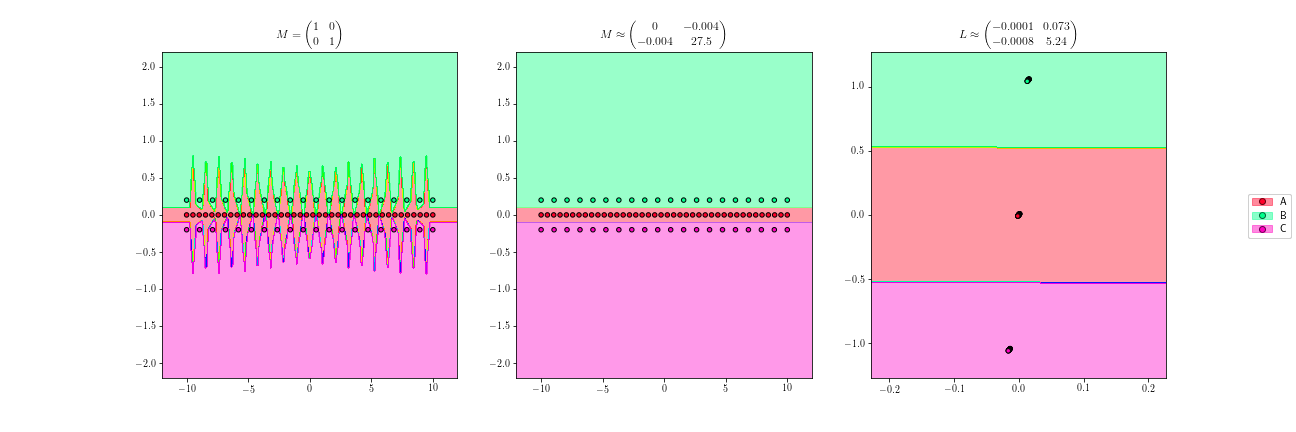
\includegraphics[width=21cm,center]{./images/ex_learning_nca.png}
    \caption{Supongamos que tenemos un conjunto de datos en el plano, los cuales pueden pertenecer a tres clases distintas, cuyas regiones vienen definidas por rectas paralelas. Supongamos que para clasificar un nuevo dato lo hacemos asignándole la clase del punto que se encuentre más cerca, para la distancia euclídea usual. Entonces, para los datos observados obtendríamos unas regiones de clasificación como las de la figura de la izquierda, pues los datos de las clases B y C están mucho más separados entre sí que la separación entre las regiones. Sin embargo, si aprendemos una distancia adecuada y volvemos a intentar clasificar asignando la clase del punto más cercano para esta nueva distancia, obtenemos unas regiones de clasificación como las de la figura central, mucho más efectivas. Por último, aprender una métrica es equivalente a aprender una transformación de los datos y medir en el espacio transformado con la distancia euclídea usual. Esto se muestra en la figura derecha. También podemos observar que los datos se están proyectando, salvo errores de precisión, sobre una recta, luego también estamos reduciendo la dimensionalidad del conjunto de datos.} \label{fig:mejorar_knn}
    \end{figure}
    
    \item \textbf{Reducción de la dimensionalidad.} Como ya hemos comentado, aprender una métrica de rango no máximo implica una reducción de dimensionalidad sobre los datos con los que trabajamos. Dicha reducción de dimensionalidad proporciona numerosas ventajas, como la reducción del coste computacional, tanto en espacio como en tiempo, de los algoritmos que se utilizarán posteriormente, o la eliminación del posible ruido introducido al tomar los datos. También, como veremos en la próxima sección, algunos algoritmos basados en distancias están expuestos a un problema denominado \emph{maldición de la dimensionalidad}. Reduciendo la dimensión de los datos, dicho problema también se hace menos grave. Por último, si se estima necesario, las proyecciones a dimensión 1,2 y 3 nos permitirían obtener representaciones visuales de nuestros datos, como se muestra en la figura \ref{fig:reduc_dim}

    \begin{figure}[h]
    \centering
    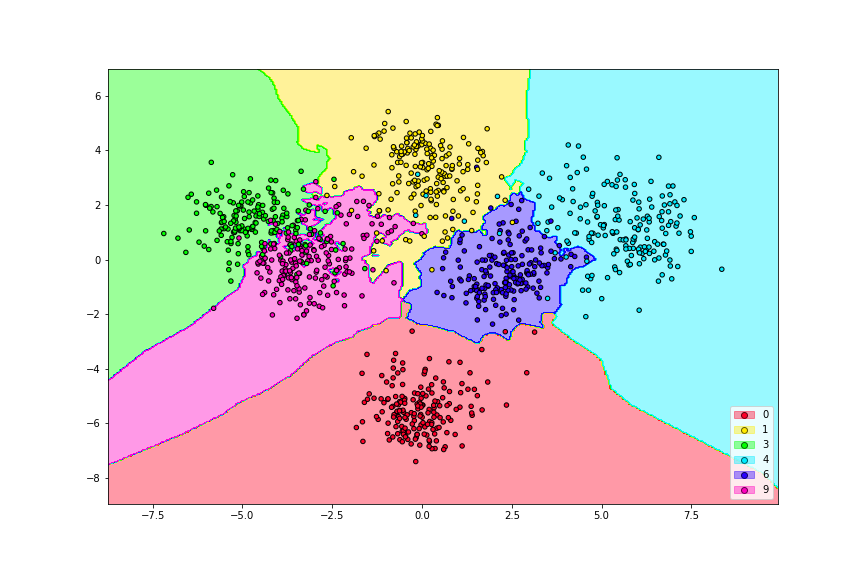
\includegraphics[width=0.75\textwidth]{./images/ex_red_dim.png}
    \caption{El dataset 'Dígitos' está formado por 1797 ejemplos. Cada uno de ellos consiste en un vector de 64 atributos, representando valores de intensidad sobre una imagen 8x8. Los ejemplos pertenecen a 10 clases distintas, cada una de ellas representando los números del 0 al 9. Aprendiendo una transformación adecuada somos capaces de proyectar la mayoría de clases sobre el plano, de forma que se perciban regiones claramente diferenciadas asociadas a cada una de las clases.} \label{fig:reduc_dim}
    \end{figure}


    \item \textbf{Cambio de ejes y reorganización de los datos.} Muy relacionada con la reducción de dimensionalidad, esta aplicación se debe a aquellos algoritmos que aprenden transformaciones que permiten mover (o seleccionar según la dimensión) los ejes de coordenadas, de forma que en el nuevo sistema de coordenadas los vectores concentren determinadas medidas de información en sus primeras componentes. Un ejemplo se muestra en la figura \ref{fig:mover_ejes}.

    \begin{figure}[h]
    \centering
    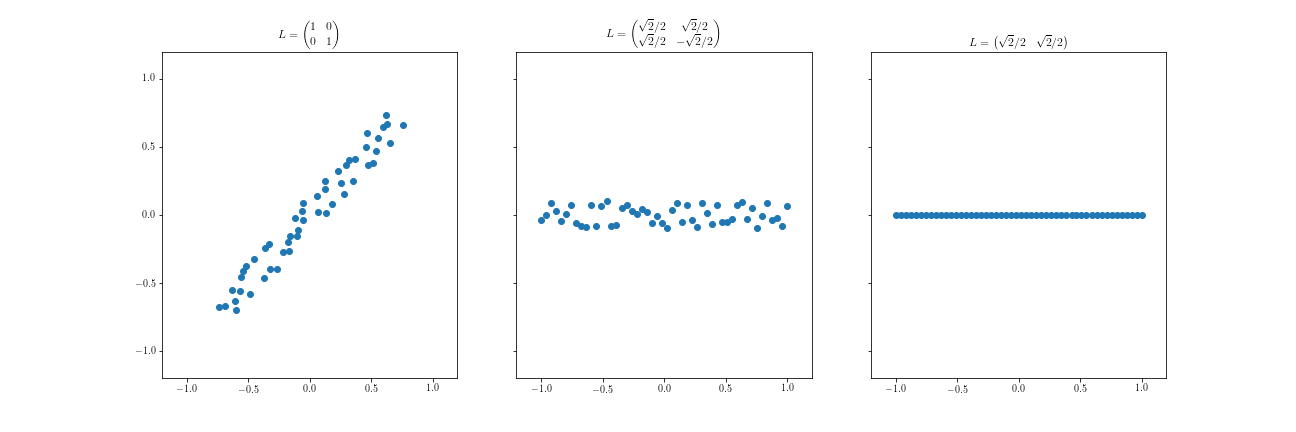
\includegraphics[width=20cm,center]{./images/ex_mover_ejes.png}
    \caption{El conjunto de datos de la figura izquierda parece que concentra la mayoría de su información en la recta diagonal que une las esquinas inferior izquierda y la superior derecha. Aprendiendo la transformación adecuada, podemos conseguir que dicha dirección caiga sobre el eje horizontal, como se muestra en la figura central. De esta forma, la primera coordenada de los vectores en esta nueva base concentra gran parte de la variabilidad del vector. Además, parece razonable pensar que los valores que introduce la coordenada vertical pueden deberse a ruido, por lo que podemos incluso quedarnos únicamente con la primera componente, como se muestra en la figura derecha.} \label{fig:mover_ejes}
    \end{figure}

    \item \textbf{Mejorar la actuación de los algoritmos de clustering.} Muchos de los algoritmos de clustering utilizan una distancia para medir la cercanía entre los datos, y así establecer los agrupamientos de forma que los datos presentes en un mismo grupo son cercanos para dicha distancia. En ocasiones, aunque desconozcamos los agrupamientos ideales de los datos ni el número de clusters a establecer, sí podemos saber que determinados pares de puntos deben estar en un mismo cluster y que otros determinados pares deben estar en clusters distintos. Esto ocurre en numerosos problemas, como por ejemplo, en el agrupamiento de documentos web. Dichos documentos poseen gran cantidad de información adicional, como es el caso de los links entre documentos, la cual nos puede incluirse como restricciones de similitud.

    \item \textbf{Aprendizaje semisupervisado.} El aprendizaje semisupervisado es un modelo de aprendizaje en el que se dispone de un conjunto de datos etiquetados y otro conjunto (en general mucho más grande) de datos sin etiquetar. Con ambos conjuntos de datos se busca aprender un modelo que permita etiquetar nuevos datos. El aprendizaje semisupervisado surge debido a que en muchas ocasiones la recopilación de datos sin etiquetar es relativamente sencilla, pero la asignación de etiquetas puede requerir que un supervisor las tenga que asignar manualmente, lo que puede ser inviable. En cambio, cuando se utilizan muchos datos no etiquetados junto con una pequeña cantidad de datos etiquetados es posible mejorar considerablemente los resultados del aprendizaje, como se ejemplifica en la figura \ref{fig:ssl}. Muchas de estas técnicas consisten en construir un grafo con aristas ponderadas a partir de los datos, donde el valor de las aristas depende de las distancias entre los datos. A partir de dicho grafo se trata de inferir las etiquetas de todo el conjunto de datos, mediante distintos algoritmos de propagación \cite{ssl1,ssl2}. En la construcción del grafo la elección de una distancia adecuada es importante, entrando así en juego el aprendizaje de métricas de distancia.

    \begin{figure}[h]
    \centering
    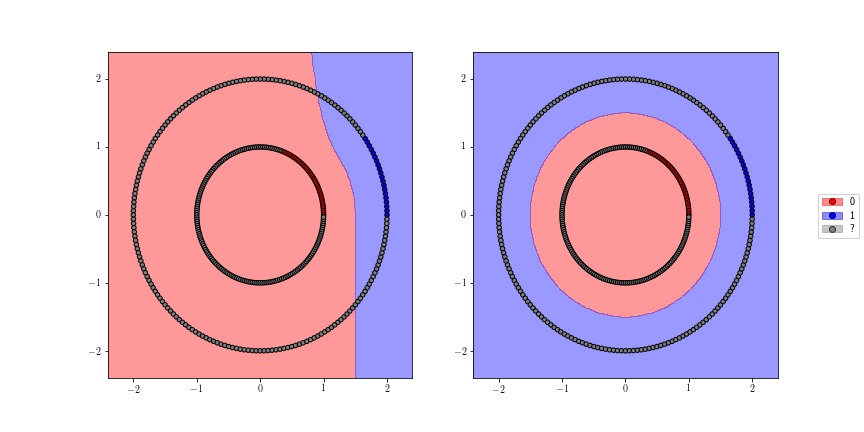
\includegraphics[width=\textwidth]{./images/ssl.png}
    \caption{Aprendizaje con la información supervisada (izquierda) frente al aprendizaje considerando toda la información no supervisada (derecha).} \label{fig:ssl}
    \end{figure}

\end{itemize}

Los algoritmos de aprendizaje supervisado analizados en este trabajo se centran en las tres primeras aplicaciones de la enumeración anterior.

\section{El aprendizaje por semejanza}

\subsection{Introducción}

El aprendizaje por semejanza es una disciplina del aprendizaje automático cuya finalidad es aprender a partir de la similitud con los datos en el conjunto de entrenamiento. De nuevo la similitud vendrá determinada por una función de distancia, por lo que el aprendizaje de una métrica apropiada previa a este proceso de aprendizaje aumentará la eficacia de este tipo de técnicas. De hecho, el aprendizaje por semejanza es una de las principales aplicaciones del aprendizaje de métricas de distancia, como se mostró en el primer ejemplo de la sección \ref{section:aplicaciones}.

En el aprendizaje supervisado, el enfoque que sigue este paradigma es el que se muestra a continuación. Supongamos que queremos aprender un clasificador para un conjunto de datos que se distribuyen de acuerdo a una distribución $\mathcal{D}$ de probabilidad. Disponemos para ello de una muestra $(x_1,y_1),\dots,(x_N,y_N)$ de datos etiquetados mediante una función de etiquetado desconocida $f\colon \mathcal{X} \to \mathcal{Y}$. Suponemos también que en el espacio $\mathcal{X}$ disponemos de una distancia $d$. Para un nuevo dato $x \sim \mathcal{D}$, le asignamos su clase a través de una función $h \colon \mathcal{X} \to \mathcal{Y}$ dada por $h(x) = \phi(d,x,(x_1,y_1),\dots,(x_N,y_N))$, una función que depende únicamente de los datos y de la distancia entre ellos.

Notemos que en este tipo de aprendizaje no buscamos un clasificador $h$ en una familia de hipótesis $\mathcal{H}$, de forma que se minimice una determinada función, sino que partimos de una función $h$ prefijada. Esto hace que el proceso de aprendizaje propiamente dicho consista únicamente en almacenar los datos en memoria, mientras que el esfuerzo computacional se realiza durante el proceso de predicción, en el que se evalúa la función de distancia. Este tipo de clasificadores, en los que el proceso de aprendizaje o generalización se retrasa hasta el momento en el que se desea predecir un nuevo dato, se denominan \emph{clasificadores perezosos}.

Por último, es interesante observar cómo el aprendizaje de métricas de distancia complementa a este tipo de clasificadores perezosos. Como ya hemos dicho, las técnicas de aprendizaje por semejanza no tienen un proceso de aprendizaje propiamente dicho y parten de una función hipótesis predefinida. En cambio, el aprendizaje de métricas de distancia sí parte de un conjunto de hipótesis, en concreto, el conjunto de distancias de Mahalanobis, como se mostraba en la expresión \ref{eq:metric_learning_eq}. Podemos combinar ambas técnicas obteniendo así un clasificador por semejanza que durante el aprendizaje encuentra una función hipótesis, dependiente de una distancia, que minimiza una función de pérdida definida para el conjunto de distancias de Mahalanobis.

El clasificador por semejanza más popular es el de vecinos cercanos, que analizaremos en la siguiente sección.

\subsection{El clasificador de vecinos cercanos.}

El clasificador de vecinos cercanos es un clasificador por semejanza muy conocido y que, como su propio nombre indica, clasifica los nuevos datos de acuerdo con la clase de sus vecinos más cercanos. Supongamos que tenemos la muestra de entrenamiento $(x_1,y_1),\dots,(x_N,y_N)$ y un dato a predecir, $x \in \mathcal{X}$. Definimos, para dicho $x$, una permutación $(\pi_1(x),\dots,\pi_N(x))$ del conjunto $\{1,\dots,N\}$ de forma que los datos de entrenamiento quedan ordenados por dicha permutación según su distancia a $x$, es decir, se tiene que
\[ d(x,x_{\pi_i}(x)) \le d(x,x_{\pi_{i+1}}(x)) \quad i=1,\dots,N-1. \]

Entonces, el clasificador de los $k$ vecinos cercanos o k-NN asigna a $x$ el valor más repetido en la lista $(y_{\pi_1(x)},\dots,y_{\pi_k(x)})$, es decir, la clase mayoritaria de sus $k$ vecinos más cercanos. Cuando $k=1$, la función hipótesis $h$ viene dada por $h(x) = y_{\pi_1}(x)$. En este caso, las regiones que determinan cada posible vecino más cercano vienen determinadas por politopos convexos (la generalización de polígonos y poliedros) y se denominan celdas de Voronoi. En el caso bidimensional, las regiones se pueden visualizar mediante diagramas de Voronoi (figura \ref{fig:voronoi}).

\begin{figure}[h]
    \centering
    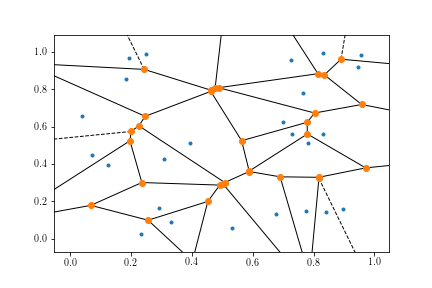
\includegraphics[width=0.5\textwidth]{./images/voronoi.png}
    \caption{Diagrama de Voronoi.} \label{fig:voronoi}
\end{figure}

Es interesante destacar que, por cómo se asignan las clases para los nuevos datos, el k-NN permite trabajar en problemas de clasificación multiclase sin ningún tipo de limitación. Esto, normalmente, no es así para muchos clasificadores, los cuales están diseñados únicamente para resolver problemas de clasificación binarios. Para extender estos clasificadores a problemas multiclase, la estrategia más común es dividir el problema en subproblemas binarios, resolver estos problemas, y asignar la clase final como aquella mayoritaria obtenida en los subproblemas. Los métodos usuales de división en problemas binarios consisten en enfrentar una clase frente a todas las demás (\emph{One versus All}), o enfrentar todos los pares de clases entre sí (\emph{One versus One}) \cite{ovoova}. En general, la mayoría de técnicas que aprenden por semejanza permiten también trabajar directamente con problemas multiclase.

La elección del número de vecinos $k$ puede influir bastante en la región delimitada por el clasificador. Dicha región es no paramétrica, al no hacerse ninguna asunción sobre la forma de la función hipótesis $h$. Los valores pequeños de $k$  se ajustan más a los datos de entrenamiento, generando así una región más puntiaguda. En tales casos, el sesgo es bajo pero la variabilidad es alta. Los papeles se intercambian para valores grandes de $k$, donde la región generada presenta un aspecto más suave, como se muestra en la figura \ref{fig:knn_comp_k}.

\begin{figure}[h]
    \centering
    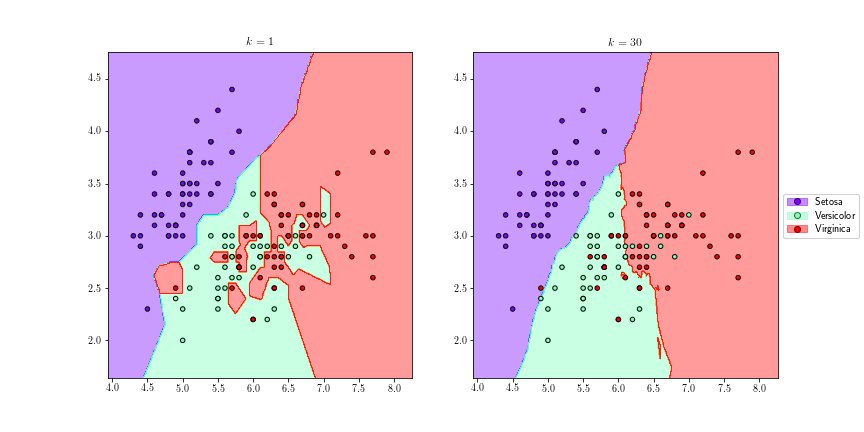
\includegraphics[width=\textwidth]{./images/compare_knn.png}
    \caption{Comparación del k-NN para distintos valores de $k$ (dataset 'Iris')} \label{fig:knn_comp_k}
\end{figure}

Como ya se anticipó en la sección, el k-NN sufre de la conocida como \emph{maldición de la dimensionalidad}. Nos restringimos al caso $k=1$. Supongamos que el dominio del problema es $\mathcal{X} = [0,1]^d$ (es decir, trabajamos con datos normalizados) y suponemos que el conjunto de clases es $\mathcal{Y} = \{0,1\}$. Suponemos que $\mathcal{D}$ es una distribución sobre $\mathcal{X}\times\mathcal{Y}$ para la cual la distribución de probabilidad condicionada, $\eta(x) = \mathbb{P}[y=1|x]$ es $c$-lipschitziana para la distancia $d$ con la que trabajamos. Entonces, es posible probar que la diferencia entre el error empírico y el \emph{error bayesiano óptimo}, asociado a la hipótesis $h^*(x) = \mathbbm{1}_{[\eta(x) > 1/2]}$ puede acotarse por $4c \sqrt{d} N^{-\frac{1}{d+1}}$ \cite{understandingml}, donde $N$ es el tamaño del conjunto de entrenamiento. Por tanto, si queremos asegurar que dicho error sea menor que $\varepsilon$, necesitamos escoger $N \ge (4c\sqrt{d}/\varepsilon)^{d+1}$. Es decir, según esta cota, el número de ejemplos crece exponencialmente con la dimensionaldad del conjunto. Además, es posible encontrar distribuciones para las cuales esta cota sea necesaria, además de suficiente. Esta circunstancia se puede generalizar para cualquier $k$, y es lo que se conoce como la maldición de la dimensionalidad para el k-NN. 

Por último, es importante comentar que se puede cambiar la regla de clasificación del k-NN. Por ejemplo para, en lugar de asignar la clase mayoritaria en los $k$ vecinos más cercanos, establecer una ponderación sobre cada vecino de forma inversamente proporcional a la distancia, teniendo así más peso las clases de los primeros vecinos más cercanos. También se puede extender esta regla a problemas de regresión, considerando por ejemplo la media, o una media ponderada, entre los $k$ vecinos más cercanos. En general, un clasificador o regresor de $k$ vecinos cercanos utiliza una función hipótesis que se puede expresar genéricamente como
\[ h(x) = \phi(x,d,(x_{\pi_1(x)},y_{\pi_1(x)}),\dots,(x_{\pi_N(x)},y_{\pi_N(x)})). \]

\subsection{Otros clasificadores por semejanza.}

Aunque el k-NN es el algoritmo por semejanza más popular para clasificación, no es el único. A continuación se muestran otros clasificadores relevantes.

\begin{itemize}
    \item \textbf{El clasificador de la media más cercana.} Denominado NCM (\emph{Nearest Class Mean}), este clasificador, durante el proceso de aprendizaje, calcula los vectores media de cada clase. Después, a la hora de predecir un nuevo dato, le asigna la clase del vector media más cercano. Es un clasificador muy eficiente y simple, aunque su simplicidad lo convierte en un clasificador bastante débil frente a conjuntos que no se agrupan en torno a su media. Existe la posibilidad de generalizarlo a múltiples centroides, como veremos en la sección \ref{section:ncmc}.

    \item \textbf{El clasificador de vecinos cercanos por radio}. Este clasificador es muy similar al k-NN, solo que en este caso, en vez de fijar un número de vecinos $k$, se fija un radio $R$. A la hora de clasificar un nuevo dato $x$, se buscan todos los datos del conjunto de entrenamiento que disten de $x$ menos que $R$. Todos los datos encontrados serán los vecinos cercanos de $x$, y a $x$ se le asignará la clase mayoritaria entre dichos vecinos. Notemos que en este caso, el número de vecinos varía con cada ejemplo, pudiendo incluso no haber vecinos. En este caso, la elección de un radio adecuado es muy importante, y puede presentar un comportamiento inadecuado en conjuntos de datos con grandes variaciones de densidad (podría haber zonas en las que apenas hay vecinos y zonas con un número elevado de vecinos).


\end{itemize}

\begin{comment}
\subsection{Fundamentos estadísticos del k-NN. La maldición de la dimensionalidad.}
\end{comment}


%% CAPÍTULO 6 - DESCRIPCIÓN DE TÉCNICAS DE APRENDIZAJE DE MÉTRICAS DE DISTANCIA
\chapter{Descripción teórica de técnicas de aprendizaje de métricas de distancia} \label{chapter:dml_algorithms}

En este capítulo se describen algunas de las técnicas más populares actualmente en el aprendizaje de métricas de distancia supervisado. A ellas se añade el análisis de componentes principales, pese a no ser supervisado, debido a su importancia para otros algoritmos de aprendizaje de métricas. Algunas estas técnicas, como PCA o LDA, constituyen procedimientos estadísticos desarrollados a finales del siglo pasado, que en la actualidad siguen siendo de gran relevancia en muchos problemas. Otras propuestas más recientes se sitúan en el estado del arte, como es el caso de NCMML o DMLMJ, entre otras.

Las técnicas analizadas se agrupan en seis secciones. Cada una de estas secciones describe algoritmos que comparten una misma finalidad principal, si bien las finalidades que describen cada sección no son exclusivas. En la primera sección se estudian las técnicas orientadas específicamente a la reducción de dimensionalidad. A continuación, se desarrollan las técnicas cuya finalidad es aprender distancias que mejoren el clasificador kNN, seguidas de aquellas que buscan mejorar los clasificadores basados en centroides. La cuarta sección incluye los métodos basados en la teoría de la información, especialmente en las divergencias, aprendiendo así distancias que acerquen o alejen determinadas distribuciones de probabilidad según la divergencia medida. Posteriormente se describen varios mecanismos de aprendizaje de distancias con objetivos menos específicos. Por último, se analizan las versiones basadas en kernels de algunos de los algoritmos anteriores, para trabajar en espacios de alta dimensionalidad.

Para cada una de las técnicas se analizará el problema que buscan resolver u optimizar, las formulaciones matemáticas de dichos problemas y los algoritmos propuestos para resolverlos.

\section{Técnicas de reducción de dimensionalidad}

\subsection{PCA}

El \emph{análisis de componentes principales} (PCA, \emph{Principal Component Analysis}) es una de las técnicas más populares de reducción de dimensionalidad en el ámbito del aprendizaje de métricas de distancia. Aunque se trata de una técnica de aprendizaje sin ningún tipo de supervisión, resulta necesario hablar de ella en este trabajo, por un lado por su gran relevancia, y más en particular, porque PCA es la herramienta de reducción de dimensionalidad por excelencia utilizada en los algoritmos de aprendizaje de distancias supervisados que no admiten de por sí una reducción de dimensionalidad. En tales algoritmos, PCA se aplica primeramente sobre los datos para poder utilizar posteriormente el algoritmo en el espacio de dimensión reducida.

El análisis de componentes principales puede entenderse desde dos puntos de vista diferentes, que acaban conduciendo al mismo problema de optimización. El primero de estos enfoques consiste en encontrar dos transformaciones, una que comprima los datos a un espacio de menor dimensión, y otra que los descomprima en el espacio original, de forma que en el proceso de compresión y descompresión se pierda la mínima información.

Vamos a centrarnos en este primer enfoque. Supongamos que tenemos el conjunto de datos $\mathcal{X} = \{x_1,\dots,x_N\} \subset \mathbb{R}^d$, y fijamos $d' < d$. Vamos a suponer además que los datos están centrados, es decir, que su media es cero. Si no lo fuera, basta con aplicar previamente a los datos la transformación $x \mapsto x - \mu$, donde $\mu = \sum x_i / N$ es la media de los datos. Buscamos una matriz de compresión $L \in \mathcal{M}_{d'\times d}(\R)$ y una matriz de descompresión $U \in \mathcal{M}_{d\times d'}(\R)$ de forma que, tras comprimir y descomprimir cada dato, los cuadrados de las distancias euclídeas al dato original sean mínimos. Es decir, el problema que buscamos resolver es

\begin{equation} \label{eq:pca:compress}
    \min_{\substack{L \in \mathcal{M}_{d'\times d}(\R) \\ U \in \mathcal{M}_{d\times d'}(\R)}} \quad \sum_{i=1}^{N} \|x_i - ULx_i\|_2^2.
\end{equation}

Para encontrar una solución a este problema, en primer lugar vamos a ver que las matrices $U$ y $L$ han de estar relacionadas de una forma muy particular.

\begin{lem}
    %% **** Tal vez seria mejor poner existe una solucion (U,L) del problema tal que ...
    Si $(U,L)$ es una solución del problema \ref{eq:pca:compress}, entonces $LL^T = I$ (en $\mathbb{R}^{d'}$) y $U = L^T$.
\end{lem}

\begin{proof}
    Fijamos $U \in \mathcal{M}_{d\times d'}(\R)$ y $L \in \mathcal{M}_{d'\times d}(\R)$. Podemos suponer que tanto $U$ como $L$ tienen rango máximo, pues en caso contrario el rango de $UL$ es menor que $d'$. Notemos que en tal caso, siempre es posible extender las matrices $U$ y $L$ a rango máximo de forma que el subespacio generado extienda al generado por $UL$ (basta sustituir los vectores linealmente dependientes en las columnas de la matriz por vectores independientes mientras la dimensión lo permita), y en tal caso el error obtenido en \ref{eq:pca:compress} para la extensión va a ser, a lo sumo, el error obtenido para $U$ y $L$.

    Consideramos la aplicación $x \mapsto ULx$. La imagen de esta aplicación, $R = \{ ULx \colon x \in \R^d \}$, es un subespacio vectorial de $\R^d$ de dimensión $d'$. Sea $\{u_1,\dots,u_{d'}\}$ una base ortonormal de $R$, y sea $V \in \mathcal{M}_{d'\times d}(\R)$ la matriz que tiene, por filas, los vectores $u_1,\dots,u_{d'}$. Se verifica entonces que la imagen de $V$ tiene rango $d'$ y que $VV^T = I$. Además, si consideramos $V^T$ como aplicación lineal, se tiene que su imagen es $R$ (puesto que $V^Te_i = u_i, i = 1,\dots,d'$, donde $\{e_1,\dots,e_{d'}\}$ es la base usual de $\mathbb{R}^{d'}$).

    Por tanto, todos los vectores de $R$ pueden escribirse como $V^Ty$, con $y \in \mathbb{R}^{d'}$. Dados $x \in \R^d, y \in \R^{d'}$, se tiene
    \begin{align*}
    \|x-V^Ty\|_2^2 &= \langle x- V^Ty, x - V^Ty \rangle \\
                   &= \|x\|^2 - 2\langle x,V^T y\rangle + \|V^Ty\|^2 \\
                   &= \|x\|^2 - 2\langle y,Vx \rangle + y^TVV^Ty \\
                   &= \|x\|^2 - 2\langle y,Vx \rangle + y^Ty \\
                   &= \|x\|^2 + \|y\|^2 - 2 \langle y,Vx \rangle.
    \end{align*}

    Si calculamos el gradiente respecto de $y$ a partir de la última expresión anterior, obtenemos $\nabla_y \|x-V^Ty\|_2^2 = 2y - 2Vx$, que, al igualar a cero, nos permite obtener un único punto crítico, $y = Vx$. La convexidad de esta función (es la composición de la norma euclídea con una aplicación afín) nos asegura que este punto crítico es un mínimo global. Por tanto, esto nos indica que, para cada $x \in \R^d$, la distancia a $x$ en el conjunto $R$ alcanza su mínimo en el punto $V^TVx$. En particular, para los datos del conjunto $\mathcal{X}$ concluimos que
    \[ \sum_{i=1}^N \|x_i - ULx_i\|_2^2 \ge \sum_{i=1}^N\|x_i - V^TV x_i\|^2_2. \]

    Podemos encontrar una matriz $V$ con estas propiedades para cualesquiera $U$ y $L$ en las condiciones del problema, lo que concluye la prueba.
\end{proof}

El lema anterior nos permite reformular nuestro problema en términos únicamente de la matriz $L$,

\begin{equation} \label{eq:pca:compress2}
    \min_{\substack{L \in \mathcal{M}_{d'\times d}(\R) \\LL^T = I}} \quad \sum_{i=1}^{N} \|x_i - L^TLx_i\|_2^2.
\end{equation}

Notemos ahora que, para $x \in \R^d$ y $L \in \mathcal{M}_{d'\times d}(\R)$ con $LL^T = I$, se verifica
\begin{align*}
    \|x - L^TLx\|_2^2 &= \langle x - L^TLx, x - L^TLx \rangle \\
                      &= \|x\|^2 - 2\langle x,L^TLx \rangle + \langle L^TLx, L^TLx \rangle \\
                      &= \|x\|^2 - 2x^TL^TLx + x^TL^TLL^TLx \\
                      &= \|x\|^2 - x^TL^TLx \\
                      &= \|x\|^2 - \tr(x^TL^TLx) \\
                      &= \|x\|^2 - \tr(Lxx^TL^T).
\end{align*}

Por tanto, si eliminamos los términos que no dependen de $L$, podemos transformar el problema \ref{eq:pca:compress2} en el siguiente problema equivalente:
\begin{equation} \label{eq:pca:traceproblem}
    \max_{\substack{L \in \mathcal{M}_{d'\times d}(\R) \\LL^T = I}} \quad \tr\left(L \Sigma L^T\right),
\end{equation}

donde $\Sigma = \sum_{i=1}^N x_ix_i^T$ es, salvo una constante, la matriz de covarianza asociada a los datos de $\mathcal{X}$. Esta matriz es simétrica, y el teorema \ref{thm:eigen_trace_opt} garantiza que podemos encontrar un máximo del problema si construimos $L$ añadiendo los $d'$ vectores propios de $\Sigma$ correspondientes a sus $d'$ mayores valores propios. Estos vectores los podemos tomar ortonormales, por la simetría de $\Sigma$. Las direcciones que determinan estos vectores son las \emph{direcciones principales}, y las componentes de los datos transformados en el sistema ortonormal determinado por las direcciones principales son las llamadas \emph{componentes principales}.

Para concluir, el segundo enfoque desde el que se puede tratar el problema de los componentes principales consiste en la selección de las direcciones ortogonales para las que se maximice la varianza. Sabemos que si $\Sigma$ es la matriz de covarianza de $\mathcal{X}$, al aplicar una transformación $L$ a los datos la nueva matriz de covarianza viene dada por $L\Sigma L^T$. Si queremos una transformación que reduzca la dimensionalidad y para la cual se maximice la varianza en cada variable lo que buscamos es tomar la traza de la matriz anterior, lo que nos conduce de nuevo al problema \ref{eq:pca:traceproblem}. La simetría de $\Sigma$ garantiza que podamos tomar las direcciones principales ortonormales que maximicen la varianza para cada posible valor de $d'$.

Por último, es importante destacar que la matriz $L \in \mathcal{M}_{d}(\R)$ (tomando todas las dimensiones) que se construye añadiendo por filas los vectores propios de $\Sigma$ es la matriz ortonormal que diagonaliza $\Sigma$, y por tanto, al aplicar $L$ sobre los datos, los datos transformados tienen como matriz de covarianza la matriz diagonal $L\Sigma L^T = \diag(\lambda_1,\dots,\lambda_d)$, donde $\lambda_1,\dots,\lambda_d$ son los valores propios de $\Sigma$. Esto nos dice que los valores propios de la matriz de covarianza representan la cantidad de varianza explicada por cada una de las direcciones principales. Esto proporciona una ventaja adicional al PCA, ya que permite analizar el porcentaje de varianza que explica cada componente principal para poder a posteriori elegir una dimensión que se ajuste a la cantidad de varianza que se quiera conservar en los datos transformados.

La Figura \ref{fig:pca} ejemplifica gráficamente el funcionamiento del análisis de componentes principales.

\begin{figure}[h]
    \centering
    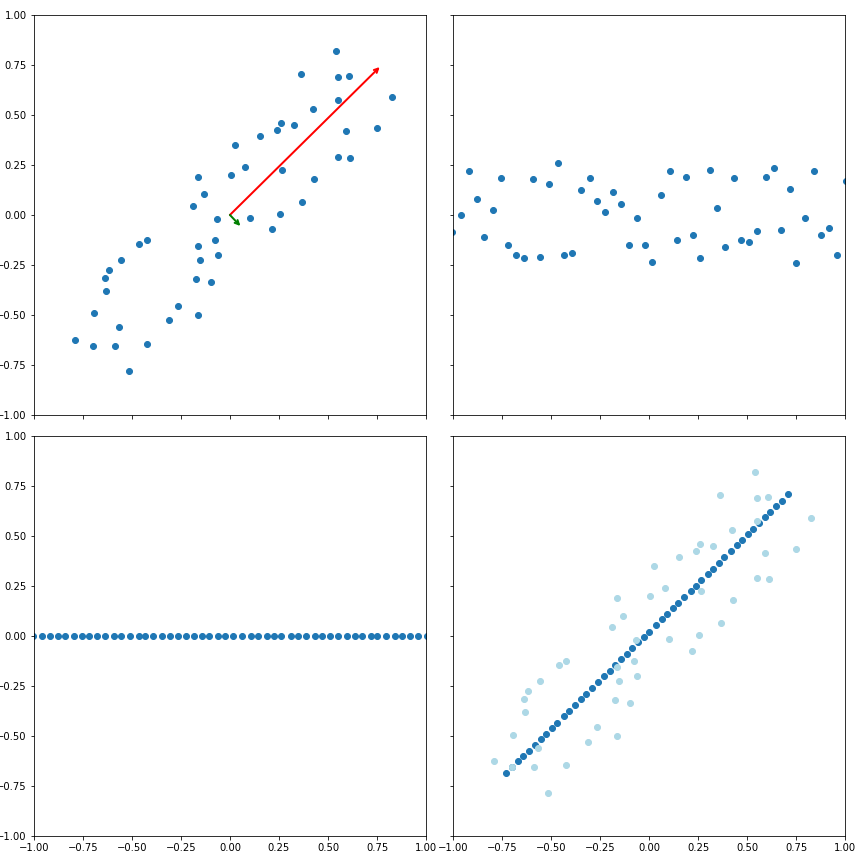
\includegraphics[width=0.75\textwidth]{./images/pca.png}
    \caption{Ejemplificación gráfica del PCA. En la primera imagen se muestra un conjunto de datos, junto con las direcciones principales (proporcionales de acuerdo a la varianza explicada) aprendidas por PCA. A su derecha, los datos proyectados en dimensión máxima. Observamos que dicha proyección consiste en girar los datos haciendo coincidir los ejes con las direcciones principales. Abajo a la izquierda, los datos proyectados sobre la primera componente principal. Por último, a su derecha, los datos recuperados mediante la matriz de descompresión, junto con los datos originales. Podemos comprobar que la proyección de PCA es la que minimiza el error cuadrático de descompresión. En este caso particular los datos descomprimidos se encuentran en la recta de regresión de los datos originales, debido a las dimensiones del problema.} \label{fig:pca}
\end{figure}

%% **** Figura(s) explicativa(s)

\subsection{LDA}

El análisis discriminante lineal (LDA, \emph{Linear Discriminant Analysis}) es una técnica clásica de aprendizaje de métricas de distancia cuya finalidad es aprender una matriz de proyección que maximice la separación entre clases en el espacio proyectado, es decir, trata de encontrar las direcciones que mejor permiten distinguir las distintas clases, como se muestra en la Figura \ref{fig:lda}.

\begin{figure}[h]
    \centering
    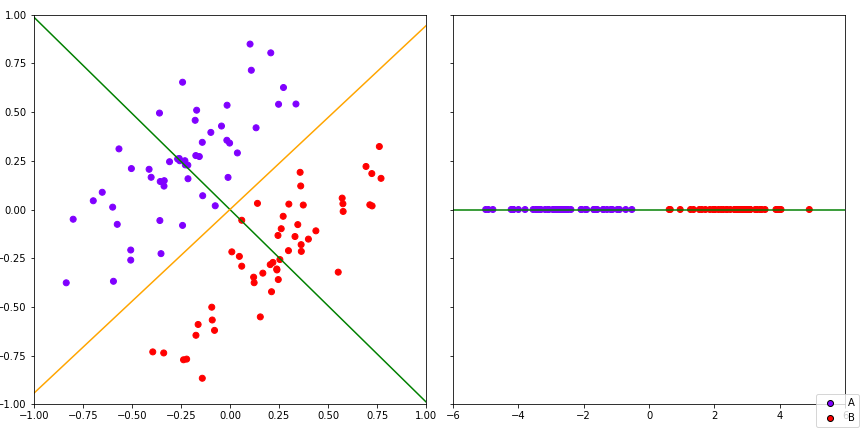
\includegraphics[width=0.75\textwidth]{./images/lda.png}
    \caption{Ejemplo gráfico del LDA y comparación con PCA. En la primera imagen se muestra un conjunto de datos, con la dirección principal determinada por PCA, en naranja, y la dirección determinada por LDA, en verde. Observamos que si proyectamos los datos sobre la dirección obtenida por LDA quedan bien separados, como se muestra en la imagen derecha. En cambio, la dirección obtenida por PCA solo nos permite maximizar la varianza de todo el conjunto al proyectar, pues no considera la información de las etiquetas.} \label{fig:lda}
    %
\end{figure}


La Figura \ref{fig:lda} nos permite, además, comparar los resultados de las proyecciones obtenidas por PCA y LDA, mostrando la diferencia más notable entre ambas técnicas: PCA no tiene en cuenta la información de las clases, buscando las direcciones que maximizan la varianza del conjunto total de datos, mientras que LDA sí que utiliza la información presente en las etiquetas, obteniendo direcciones en las que mejor se pueden proyectar los datos para tener una buena separación de clases. Se puede apreciar que las direcciones obtenidas por PCA y LDA no presentan ningún tipo de relación, siendo esta última la única de las dos que proporciona una proyección de los datos orientada al aprendizaje supervisado. 

También es posible observar en la Figura \ref{fig:lda} que no tiene sentido buscar una segunda dirección independiente que siga maximizando la separación de las clases, mientras que en PCA siempre tiene sentido ir buscando inductivamente direcciones ortogonales que maximicen la varianza. Si el conjunto de datos mostrado en la figura tuviera una tercera clase, podríamos encontrar una segunda dirección que maximizara la separación entre clases, ofreciendo así la posibilidad de proyectar sobre el plano. En general, vamos a ver que si tenemos $r$ clases podremos encontrar como mucho (y siempre que lo permita la dimensión del espacio original) $r-1$ direcciones que maximicen la separación. Esto nos indica que las proyecciones que va a aprender LDA van a ser, en general, hacia una dimensión bastante baja, y siempre limitada por el número de clases en el conjunto de datos.

Supongamos el conjunto de datos etiquetados $\mathcal{X} = \{x_1,\dots,x_N\} \subset \R^d$ donde $\mathcal{C}$ es el conjunto de clases del problema, e $y_1,\dots,y_N \in \mathcal{C}$ son las etiquetas asociadas a cada dato de $\mathcal{X}$. Supongamos que el número de clases del problema es $|\mathcal{C}| = r$. Para cada $c \in \mathcal{C}$ definimos el conjunto $\mathcal{C}_c = \{ i \in \{1,\dots,N\} \colon y_i = c \}$, y $N_c = |\mathcal{C}_c|$. Consideramos los vectores media de cada clase,
\[\mu_c = \frac{1}{N_c} \sum_{i \in \mathcal{C}_c} x_i,\]
y el vector media de todo el conjunto de datos,
\[\mu = \frac{1}{N}\sum_{c \in \mathcal{C}}\sum_{i \in \mathcal{C}_c}x_i = \frac{1}{N}\sum_{i=1}^N x_i. \]

Vamos a definir dos matrices de dispersion, una entre clases (denominada \emph{between-class}), y otra entre los datos de mismas clases o intra-clase (denominada \emph{within-class}), notadas como $S_b$ y $S_w$, respectivamente. La matriz de dispersión entre clases se define como
\begin{equation}
    S_b = \sum_{c \in \mathcal{C}} N_c(\mu_c - \mu)(\mu_c - \mu)^T.
\end{equation}
Y la matriz de dispersión intra-clase,
\begin{equation}
    S_w = \sum_{c \in \mathcal{C}} \sum_{i \in \mathcal{C}_c}(x_i- \mu_c)(x_i - \mu_c)^T.
\end{equation}  

Notemos que estas matrices, representan, salvo constantes multiplicativas, las covarianzas entre los datos de las distintas clases tomando las medias como representantes de cada clase en el primer caso, y la suma, para cada clase, de las covarianzas para los datos de dicha clase, en el segundo caso. Como queremos maximizar la separación vamos a formular el problema de optimización como la búsqueda función de una proyección $L \in \mathcal{M}_{d'\times d}(\R)$ que maximice el cociente entre las varianzas entre clase y las varianzas intra clase determinadas por las matrices anteriores. El problema se establece como
\begin{equation} \label{eq:lda}
    \max_{\substack{L \in \mathcal{M}_{d'\times d}(\R) }} \quad \tr\left((LS_wL^T)^{-1}(L S_b L^T)\right).
\end{equation}


El teorema \ref{thm:eigen_trace_ratio_opt} nos asegura que para maximizar el problema \ref{eq:lda} $L$ ha de estar compuesta por los vectores propios asociados a los valores propios de mayor valor de $S_w^{-1}S_b$, siempre que $S_w$ sea invertible. En la práctica, esto ocurre en la mayoría problemas donde $N \gg d$, pues $S_w$ es la suma de $N$ productos tensoriales, cada uno de los cuales puede aportar una dimensión al rango. Si $N \gg d$ es probable que $S_w$ tenga rango máximo. Esto, junto a que $S_w$ es semidefinida positiva garantizarían que $S_w$ fuera definida positiva, entrando así en las hipótesis del teorema.

Es interesante destacar el parecido entre el problema de optimización \ref{eq:lda} y la expresión del índice de Calinski-Harabasz \cite{maulik2002performance}, un índice utilizado en clustering para medir la separación de las clases establecidas.

Por otra parte, notemos, como ya se adelantó al inicio de la sección, que a lo sumo podemos obtener $r-1$ vectores propios con valor propio asociado no nulo. Esto es debido a que $S_b$ tiene a lo sumo rango $r-1$, pues su rango coincide con el rango de la matriz $A$ que tiene por columnas los vectores $\mu_c - \mu$ (se verifica que $S_b = A \diag(N_{c_1},\dots,N_{c_r}) A^T$), lo que da como rango a lo sumo $r$, y dicha matriz presenta además la combinación lineal $\sum N_c(\mu_c- \mu) = 0$. Por tanto, $S_w^{-1}S_b$ también tiene a lo sumo rango $r-1$. En consecuencia, la matriz de proyección que maximiza el problema \ref{eq:lda} también va a tener, a lo sumo, este rango, luego la proyección va a quedar contenida en un espacio de dicha dimensión. Por tanto, la elección de una dimensión $d' > r-1$ no va a aportar ninguna información adicional a la que aporta la proyección en dimensión $r-1$.

Para concluir, aunque hemos visto que LDA permite reducir la dimensionalidad añadiendo información supervisada frente a la no supervisión de PCA, también puede presentar algunas limitaciones:

\begin{itemize}
 \item Si la muestra de datos es demasiado pequeña, la matriz de dispersión intra-clase puede ser singular, impidiendo el cálculo de $S_w^{-1}S_b$. En esta situación, se han propuesto diversos mecanismos para seguir adelante con esta técnica. Uno de los más utilizados consiste en regularizar el problema, considerando, en lugar de $S_w$, la matriz $S_w + \varepsilon I$, donde $\varepsilon > 0$, haciendo que $S_w + \varepsilon I$ sea definida positiva. El problema de la singularidad de $S_w$ también surge si hay atributos correlacionados. Este caso se puede evitar eliminando atributos redundantes en un preprocesado previo al aprendizaje.

 \item La definición de las matrices de dispersión asume en cierta medida que los datos en cada clase se distribuyen mediante gaussianas multivariante. Por tanto, si los datos presentaran otras distribuciones, la proyección aprendida podría no ser de calidad.

 \item Como ya se ha comentado, LDA solo permite la extracción de $r-1$ atributos, lo cual puede ser subóptimo en algunos casos, pues se podría perder bastante información.
\end{itemize}


\subsection{ANMM}

ANMM (\emph{Average Neighbor Margin Maximization}) \cite{anmm} es una técnica de aprendizaje de métricas de distancia orientada específicamente a la reducción de dimensionalidad. Sigue por tanto el mismo camino que los ya comentados PCA y LDA, intentando solventar algunas de las limitaciones que presentan estos últimos.

El objetivo de ANMM es aprender una transformación lineal $L \in \mathcal{M}_{d'\times d}(\mathbb{R})$, con $d' \le d$,  que proyecte los datos a un espacio de menor dimensión, de forma que se maximice la similitud entre elementos de la misma clase y la separación entre elementos de distintas clases, siguiendo el criterio de maximización de márgenes que vamos a mostrar a continuación.

Consideramos el conjunto de datos de entrenamiento $\mathcal{X} = \{x_1,\dots,x_N\} \subset \mathbb{R}^d$, con etiquetas $y_1,\dots,y_N$, y fijamos $\xi, \zeta \in \N$, y la distancia euclídea como distancia inicial. A partir de estas variables vamos a construir dos tipos de vecindarios.

\begin{definition}
    Sea $x_i \in \mathcal{X}$.
    
    Se define el \emph{$\xi$-vecindario homogéneo más cercano} de $x_i$ como el conjunto de los $\xi$ datos más cercanos a $x_i$ que están en su misma clase. Lo notaremos por $\mathcal{N}_i^o$.
    
    Se define el \emph{$\zeta$-vecindario heterogéneo más cercano} de $x_i$ como el conjunto de los $\zeta$ datos más cercanos a $x_i$ que están en clases distintas a la de $x_i$. Lo notaremos por $\mathcal{N}_i^e$.
\end{definition} 

Lo que va a tratar de maximizar ANMM es el concepto de margen promedio de vecindario, que definimos a continuación.

\begin{definition}
    Dado $x_i \in \mathcal{X}$, se define su margen promedio de vecindario, y se nota $\gamma_i$, como
    \begin{equation}
        \gamma_i = \sum\limits_{k \colon x_k \in \mathcal{N}_i^e} \frac{\|x_i - x_k \|^2}{|\mathcal{N}_i^e|} - \sum\limits_{j \colon x_j \in \mathcal{N}_i^o} \frac{\|x_i - x_j \|^2}{|\mathcal{N}_i^o|}.
    \end{equation}
    
    Se define el margen promedio (global) de vecindario como
    \begin{equation}
        \gamma = \sum_{i=1}^N \gamma_i.
    \end{equation}

    
\end{definition}

Observemos que, para cada $x_i \in \mathcal{X}$, su margen promedio representa la diferencia entre la distancia media de $x_i$ a sus vecinos heterogéneos y la distancia media de $x_i$ a sus vecinos homogéneos. Por tanto, la maximización de este margen permite, localmente, alejar los datos de distintas clases y atraer a aquellos de la misma clase. En la Figura \ref{fig:average_neighbor_margin} se describe gráficamente el concepto de margen promedio de vecindario.

\begin{figure}[h]
    \centering
    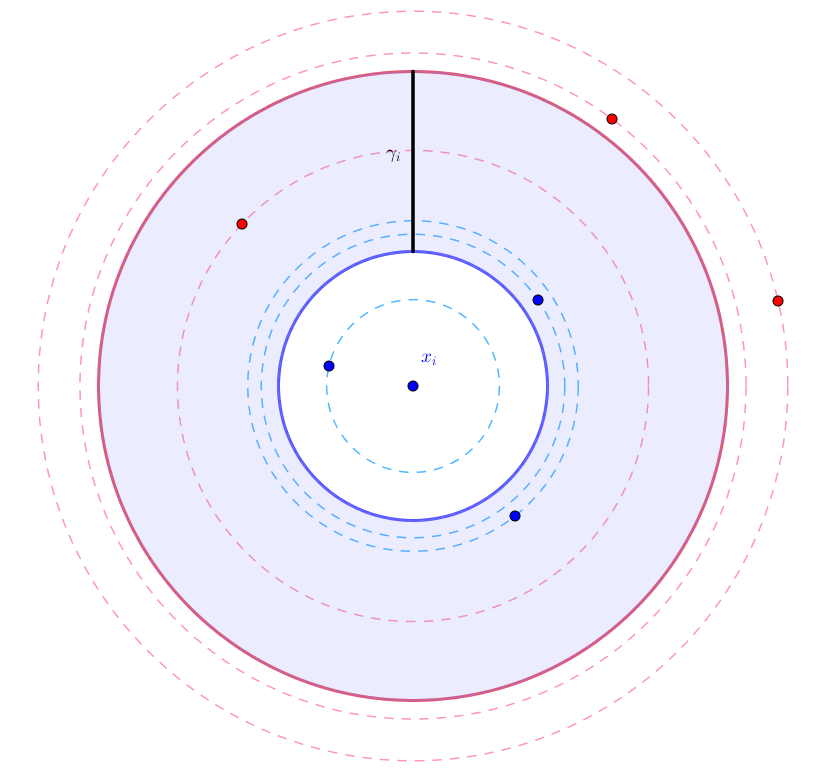
\includegraphics[width=0.55\textwidth]{./images/anmm.png}
    \caption{Descripción gráfica del margen promedio de vecindario para el dato $x_i$, para $\xi$ = $\zeta$ = 3. Las circunferencias azul y roja determinan la distancia media de $x_i$ a los datos de igual y distinta clase, respectivamente.} \label{fig:average_neighbor_margin}
\end{figure}

Buscamos ahora una transformación $L$ que maximice el margen asociado a los datos proyectados $\{Lx_i \colon i = 1,\dots,N\}$. Para tales datos, tenemos el margen asociado a dicha transformación,

\[ \gamma^L = \sum_{i=1}^{N} \gamma_i^L = \sum_{i=1}^N\left( \sum\limits_{k \colon x_k \in \mathcal{N}_i^e} \frac{\|Lx_i - Lx_k \|^2}{|\mathcal{N}_i^e|}- \sum\limits_{j \colon x_j \in \mathcal{N}_i^o} \frac{\|Lx_i - Lx_j \|^2}{|\mathcal{N}_i^o|} \right). \]

Notemos que, gracias a la linealidad de la traza, podemos expresar

\begin{align*}
    \sum_{i=1}^n\sum\limits_{k \colon x_k \in \mathcal{N}_i^e} \frac{\|Lx_i - Lx_k \|^2}{|\mathcal{N}_i^e|} &= \tr\left( \sum_{i=1}^N \sum\limits_{k \colon x_k \in \mathcal{N}_i^e} \frac{(Lx_i - Lx_k)(Lx_i - Lx_k)^T}{|N_i^e|} \right) \\
    &= \tr\left[ L \left( \sum_{i=1}^N \sum\limits_{k \colon x_k \in \mathcal{N}_i^e} \frac{(x_i-x_k)(x_i-x_k)^T}{|N_i^e|}  \right) L^T\right]\\
    &= \tr(LSL^T),
\end{align*}

donde $S = \sum_{i}\sum_{k\colon x_k \in \mathcal{N}_i^e}\frac{(x_i-x_k)(x_i-x_k)^T}{|\mathcal{N}_i^e|}$ recibe el nombre de matriz de dispersión. De la misma forma, si llamamos $C = \sum_{i}\sum_{j\colon x_j \in \mathcal{N}_i^o}\frac{(x_i-x_j)(x_i-x_j)^T}{|\mathcal{N}_i^o|}$, la cual denominaremos matriz de compacidad, se tiene que

\begin{equation*}
    \sum_{i=1}^n\sum\limits_{j \colon x_j \in \mathcal{N}_i^o} \frac{\|Lx_i - Lx_j \|^2}{|\mathcal{N}_i^o|} = \tr(LCL^T).
\end{equation*}

Y por tanto, combinando ambas expresiones,

\begin{equation} \label{eq:margin_caract}
    \gamma^L = \tr(L(S-C)L^T).
\end{equation}

La maximización de $\gamma^L$ tal como se presenta en la fórmula \ref{eq:margin_caract} no es lo suficientemente restrictiva, pues basta multiplicar $L$ por constantes positivas para obtener un valor de $\gamma^L$ tan grande como queremos. Por eso, se añade la restricción $LL^T = I$, por lo que acabamos obteniendo el siguiente problema de optimización:

\begin{align*}
    \max_{L \in \mathcal{M}_{d'\times d}(\R)} &\quad \tr\left(L(S-C)L^T\right)  \\
    \text{s.a.: } &\quad LL^T = I
\end{align*}

Notemos que $S - C$ es simétrica, pues es la diferencia de dos matrices semidefinidas positivas (cada una de ellas es suma de productos tensoriales). El teorema \ref{thm:eigen_trace_opt} nos dice que la matriz $L$ que buscamos la podemos construir añadiendo, por filas, los $d'$ vectores propios correspondientes a los $d'$ mayores valores propios de $S-C$.

Notemos que ANMM solventa alguna de las carencias de los ya vistos PCA y LDA. Por un lado, se trata de un algoritmo de aprendizaje supervisado, luego utiliza la información de las clases que es ignorada por PCA. Y frente a las carencias de LDA, podemos observar que:

\begin{itemize}
    \item No tiene problemas de cómputo con muestras pequeñas, para las cuales las matrices de dispersión o compacidad podrían resultar singulares, pues no tiene que calcular sus matrices inversas.
    \item No asume ninguna distribución sobre las clases.
    \item Admite cualquier tamaño para la reducción de dimensionalidad, no impone que dicho tamaño sea inferior al número de clases.
\end{itemize}

Por último, podemos observar también que, si mantenemos la dimensión máxima $d$, la condición $LL^T = I$ implica que $L$ es ortogonal y $L^TL=I$, luego estamos aprendiendo únicamente una isometría, como ya ocurría con PCA. Por ello, clasificadores basados en distancias como el kNN solo podrán experimentar mejoras cuando la dimensión escogida sea estrictamente menor que la original.


\section{Técnicas orientadas a la mejora del clasificador de vecinos cercanos}

\subsection{LMNN} \label{section:lmnn}

LMNN (\textit{Large Margin Nearest Neighbors}) \cite{lmnn} es un algoritmo de aprendizaje de métricas de distancia orientado específicamente a mejorar la precisión del clasificador kNN. Se basa en la premisa de que el kNN clasificará con más fiabilidad un ejemplo si sus $k$ vecinos comparten la misma etiqueta, y para ello intenta aprender una distancia que maximice el número de ejemplos que comparten etiqueta con el mayor número de vecinos posible.

De esta forma, el algoritmo LMNN trata de minimizar una función de error que penaliza, por un lado, las distancias grandes entre cada ejemplo y los considerados como sus vecinos ideales, y por otro lado, las distancias pequeñas entre ejemplos de distintas clases.

Supongamos que tenemos un conjunto de datos $\mathcal{X} = \{x_1,\dots,x_N\} \subset \mathbb{R}^d$ con etiquetas $y_1,\dots,y_N$. Para su funcionamiento, el algoritmo hace uso del concepto de \emph{vecinos objetivo} o \emph{target neighbors}. Dado un ejemplo $x_i \in \mathcal{X}$, sus $k$ vecinos objetivos son aquellos ejemplos de la misma clase que $x_i$, y distintos de este, para los que se desea que sean considerados como vecinos en la clasificación del kNN. Si $x_j$ es un vecino objetivo de $x_i$, entonces lo notaremos $j \istargetof i$. Estos vecinos objetivo están fijos durante el proceso de aprendizaje. Si se dispone de alguna información a priori se puede utilizar para determinarlos. En caso contrario, una buena opción es utilizar los vecinos cercanos de la misma clase para la distancia euclídea.

Una vez establecidos los vecinos objetivo, para cada distancia y para cada ejemplo que manejemos podemos establecer un perímetro determinado por el vecino más lejano a dicho ejemplo. Buscamos distancias para las cuales no haya ejemplos de otras clases en dicho perímetro. Hay que destacar que con este perímetro no hay suficientes garantías de separación, pues la distancia encontrada podría haber colapsado todos los vecinos objetivo en un punto y entonces el perímetro tendría radio cero. Por ello se considera un margen determinado por el radio del perímetro, al que se añade una constante positiva. Veremos que no hay pérdida de generalidad, por la función objetivo que vamos a definir, en suponer que dicha constante es 1. A cualquier ejemplo de distinta clase que invada este margen lo llamaremos \emph{impostor}. Nuestro objetivo, por tanto, será, además de acercar cada ejemplo a sus vecinos objetivo lo máximo posible, intentar alejar lo máximo posible a los impostores.

En términos matemáticos, si nuestra distancia está determinada por la aplicación lineal $L \in \mathcal{M}_{d}(\R)$, y $x_i, x_j \in \mathcal{X}$ con $j \istargetof i$, diremos que $x_l \in \mathcal{X}$ es un impostor para los datos anteriores si $y_l \ne y_i$ y $\|L(x_i - x_j)\|^2 \le \|L(x_i - x_j)\|^2+1$. En la Figura \ref{fig:targets_impostors} se describen gráficamente los conceptos de vecino objetivo e impostor. Notemos por último que el margen está definido en términos de la distancia al cuadrado, en lugar de considerar solo la distancia. Esto facilitará la resolución del problema que vamos a formular.

\begin{figure}[h]
    \centering
    \begin{subfigure}{.5\textwidth}
        \centering
        \fbox{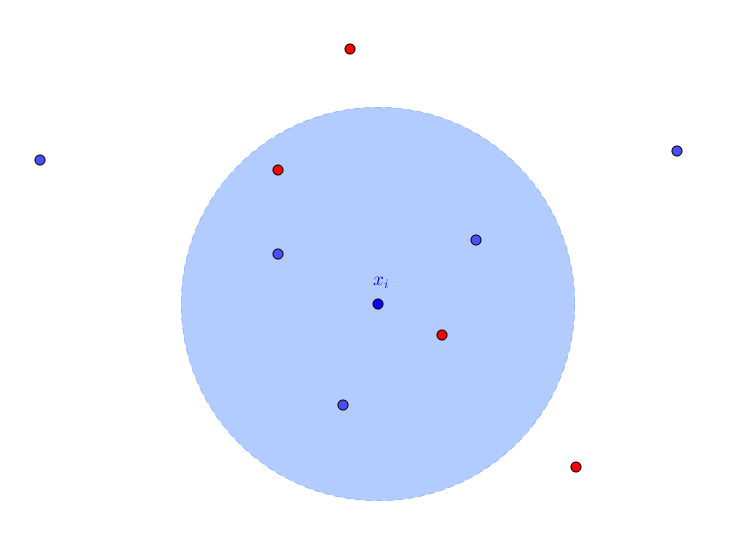
\includegraphics[height = 5cm]{images/lmnn1.png}}
    \end{subfigure}%
    \begin{subfigure}{.5\textwidth}
        \centering
        \fbox{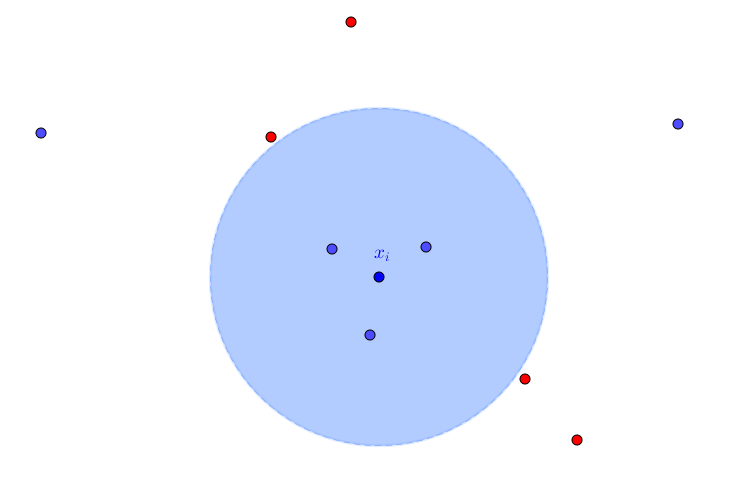
\includegraphics[height = 5cm]{images/lmnn2.png}}
    \end{subfigure}
    %\includegraphics[width=0.5\textwidth]{targets_impostors.png}
    \caption{Descripción gráfica de vecinos objetivo e impostores (para $k = 3$) para el dato $x_i$. El círculo azul representa el margen que determinan los vecinos objetivo. Todos los puntos de distintas clases en dicho círculo son impostores. El objetivo LMNN será acercar los vecinos objetivos lo máximo posible y eliminar los impostores del círculo. Por tanto, no influirán los datos de la misma clase que no sean vecinos objetivo y se dejarán de penalizar los impostores en cuanto salgan del margen, como se muestra a la derecha. Esto da un carácter local a esta técnica de aprendizaje.} \label{fig:targets_impostors}
\end{figure}

A continuación, procedemos a definir de forma precisa los términos de la función objetivo. Como ya se ha mencionado, va a estar compuesta de dos términos. El primero penalizará a los vecinos objetivo lejanos y el segundo penalizará a los impostores cercanos. El primer término se define como
\[ \varepsilon_{pull}(L) = \sum_{i=1}^N \sum_{j\istargetof i} \|L(x_i-x_j)\|^2. \]

Notemos que su minimización genera una fuerza de atracción entre los datos. El segundo término se define como
\[ \varepsilon_{push}(L) = \sum_{i=1}^{N}\sum_{j\istargetof i}\sum_{l=1}^{N} (1 - y_{il})[1 + \|L(x_i-x_j)\|^2 - \|L(x_i-x_l)\|^2]_{+}, \]

donde $y_{il}$ es una variable binaria, que vale $1$ y $y_i = y_l$ y $0$ si $y_i \ne y_l$, y el operador $[ \cdot ]_{+}\colon  \R \to \R^+_0$ se define como $[z]_{+} = \max\{z,0\}$. De esta forma, este error suma cuando $y_{il} = 0$ (es decir, $x_l$ es de distinta clase que $x_i$), y el segundo factor es estrictamente positivo (es decir, se sobrepasa el margen definido para los impostores). La minimización de este segundo término genera una fuerza de repulsión entre los datos.

Finalmente, la función objetivo resulta de combinar estos dos términos. Fijado $\mu \in ]0,1[$, definimos
\begin{equation} \label{eq:lmnn:L}
\varepsilon(L) = (1 - \mu)\varepsilon_{pull}(L) + \mu\varepsilon_{push}(L).
\end{equation}

Los autores afirman que, experimentalmente, la elección de $\mu$ no provoca grandes diferencias en los resultados, por lo que se suele tomar $\mu = 1/2$. La minimización de esta función nos llevará a aprender la distancia que buscábamos. Notemos que esta función no es convexa, por lo que si utilizamos un método de descenso bajo esta aproximación podemos quedar atrapados en un óptimo local. Sin embargo, podemos reformular nuestra función objetivo para que actúe sobre el cono de las matrices semidefinidas positivas. Si para cada $L \in \mathcal{M}_d(\R)$, tomamos $M = L^TL \in \mathcal{M}_d(\R)^+_0$, sabemos que $\|x_i-x_j\|_M^2 = \|x_i - x_j\|_L^2$, y por tanto,
\begin{equation} \label{eq:lmnn:M}
 \varepsilon(M) = (1-\mu) \sum_{i=1}^{N}\sum_{j\istargetof i} \|x_i - x_j\|_M^2 + \mu \sum_{i=1}^{N}\sum_{j\istargetof i}\sum_{l=1}^N [ 1 + \|x_i - x_j\|_M^2 - \|x_i - x_l\|_M^2]_{+}
\end{equation}

es una función convexa en $M$ que tiene toma los mismos valores que $\varepsilon(L)$. La minimización de $\varepsilon(M)$ en este caso está sujeta a la restricción $M \succeq 0$, por lo que podemos efectuarla mediante programación semidefinida, desplazándonos en la dirección del gradiente y proyectando el resultado sobre el cono semidefinido en sucesivas iteraciones. Además, podemos calcular un subgradiente $G \in \partial \varepsilon / \partial M$ dado por
\[ G = (1-\mu) \sum_{i,j\istargetof i} O_{ij} + \mu \sum_{(i,j,l) \in \mathcal{N}} (O_{ij} - O_{il}), \]

donde $\mathcal{N}$ es el conjunto de tripletas $(i,j,l)$ para las cuales $x_l$ es un impostor sobre $x_i$ con el margen determinado por $x_j$, y $O_{ij} = (x_i - x_j)(x_i - x_j)^T$ son los productos tensoriales obtenidos de derivar las distancias. El primer término del gradiente es constante, mientras que el segundo solo varía en cada iteración con los cambios de los impostores que entran o salen de el conjunto $\mathcal{N}$. Estas consideraciones permiten realizar un cálculo del gradiente bastante eficiente.

En cuanto a la reducción de dimensionalidad, se presentan dos alternativas diferentes. Si mantenemos la optimización respecto a $M$, no es factible añadir restricciones de rango y seguir obteniendo un problema de programación semidefinida. Por tanto, se propone el uso de PCA previamente a la ejecución del algoritmo, para proyectar los datos sobre sus componentes principales, y aplicar LMNN sobre los datos proyectados. La otra alternativa es optimizar la función objetivo respecto a $L \in \mathcal{M}_{d'\times d(\R)}$, con $d' < d$, usando algún algoritmo de gradiente descendente. En este caso la optimización no es convexa, pero aprendemos directamente una transformación lineal que reduce la dimensionalidad sin realizar cambios en el problema de optimización. Los autores afirman además, basados en los resultados empíricos, que esta optimización no convexa da buenos resultados.

Otras propuestas realizadas para la mejora de este algoritmo consisten en aplicar LMNN múltiples veces, aprendiendo así nuevas métricas cada vez, e ir utilizando estas métricas para determinar vecinos objetivo cada vez más precisos, o bien aprender métricas localmente. Por último, aunque la distancia aprendida está diseñada para que pueda ser utilizada por el kNN, también es posible utilizar la propia función objetivo como método para clasificar. Estos modelos de clasificación se denominan basados en energía. De este modo, para clasificar un dato test $x_t$, para cada posible valor de clase $y_t$, buscamos $k$ vecinos objetivo en el conjunto de entrenamiento de clase $y_t$, y evaluamos la \emph{energía} para la métrica aprendida, asignando finalmente a $x_t$ el valor de $y_t$ que proporcione menor energía. De acuerdo con la funión objetivo, la energía penalizará distancias grandes entre $x_t$ y sus vecinos objetivo, los impostores en el perímetro de $x_t$ y perímetros de otras clases invadidas por $x_t$. Por tanto,
\begin{equation}
\begin{split}
 y_t^{pred} &= \arg\min_{y_t} \left\{ (1-\mu) \sum_{j \istargetof t} \|x_t-x_j\|_M^2 \right. \\
            &+ \mu \sum_{j \istargetof t,l} (1-y_{tl})\left[ 1 + \|x_t-x_j\|_M^2 - \|x_t-x_l\|_M^2\right]_+  \\
            &+ \left. \mu \sum_{i,j \istargetof i}(1 - y_{it}) \left[ 1 + \|x_i-x_j\|_M^2 - \|x_i-x_t\|_M^2\right]_+ \right\} .
\end{split}
\end{equation}

\subsection{NCA}

\subsubsection{El kNN y la validación \emph{Leave One Out}}

En la mayoría de problemas de clasificación, para medir la eficacia del clasificador con el que estamos trabajando, se suele dividir el conjunto de datos del que disponemos en dos grupos: un conjunto de entrenamiento, que será el que utilice el clasificador para aprender, y un conjunto de validación, sobre el que el clasificador asigna sus predicciones, las cuales se comparan con las clases reales para evaluar el acierto del clasificador.

En algunos casos también puede resultar de interés evaluar el rendimiento del clasificador sobre los propios datos de entrenamiento, por ejemplo, para determinar si se está produciendo sobreaprendizaje, es decir, si el clasificador se adapta demasiado a los datos de entrenamiento, perdiendo así capacidad de generalización. Otra razón para ello es poder utilizar el rendimiento sobre los datos de entrenamiento como función objetivo a optimizar durante el proceso de aprendizaje. Esto contribuirá a mejorar el rendimiento del clasificador, siempre que no caiga en el sobreaprendizaje. Vamos a centrarnos en esta última razón.

En el caso del kNN, si pretendemos medir el rendimiento sobre los datos de entrenamiento, nos encontramos con un inconveniente que nos puede llevar a una interpretación incorrecta de los resultados. Y es que, para cada dato en el conjunto de entrenamiento, su vecino más cercano es él mismo, y por tanto, la clase que vaya a serle asignada va a estar condicionada por este hecho. Esto se aprecia más claramente en el caso $k=1$, donde el único vecino cercano considerado coincide siempre con el propio dato, y por tanto la tasa de acierto va a ser del 100 \%.

La forma de solucionar este inconveniente consiste en, si $\mathcal{X}$ es el conjunto de datos de entrenamiento, para cada $x \in \mathcal{X}$, obtener su predicción encontrando sus $k$ vecinos más cercanos en $X  \setminus \{x\}$. Esto es equivalente a particionar $X$ en conjuntos de un elemento, usando uno de los subconjuntos para la validación, y el resto para el entrenamiento. Este procedimiento de validación se conoce como validación cruzada \emph{Leave One Out} (LOO). Como procedimiento de validación en general, su estimación del error es poco sesgada y no tiene componente aleatoria, aunque está sometido a mayor variabilidad y es más costoso computacionalmente que otras técnicas de validación.

\subsubsection{El análisis de componentes de vecindarios}

NCA (\emph{Neighborhood Component Analysis}) \cite{nca} es un algoritmo de aprendizaje de métricas de distancia orientado específicamente a mejorar la precisión del clasificador kNN. Tiene como finalidad aprender una transformación lineal cuyo objetivo principal es minimizar el error \emph{Leave One Out} esperado por la clasificación mediante kNN. Adicionalmente, esta transformación podría usarse para reducir la dimensionalidad del conjunto de datos, y hacer por tanto más eficiente el clasificador.
    
Consideramos $\mathcal{X} = \{x_1,\dots,x_N\} \subset \mathbb{R}^d$ un conjunto de datos de entrenamiento con etiquetas $y_1,\dots,y_N$, respectivamente. Queremos aprender una distancia, determinada por una transformación lineal $L \in \mathcal{M}_{d}(\mathbb{R})$, que optimice la precisión del clasificador de vecinos cercanos. Lo ideal sería optimizar la actuación sobre los datos de validación, pero solo disponemos del conjunto de entrenamiento. Por tanto, nuestro objetivo va a ser optimizar el error \emph{Leave One Out} de clasificación sobre el conjunto de entrenamiento.

Sin embargo, la función que para cada $L$ asigna el error LOO para la distancia asociada a $L$ no tiene garantías de diferenciabilidad, ni siquiera de continuidad, por lo que no es fácil tratar con ella para su optimización (notemos que esta función toma un conjunto finito de valores y está definida en un conjunto conexo, luego no puede ser continua a menos que sea constante, lo cual no sucede en ejemplos no triviales).

Para ello, NCA trata de abordar el problema de forma estocástica, esto es, en vez de operar con el error LOO directamente, lo hace sobre su valor esperado para la probabilidad que vamos a definir a continuación.

Dados dos ejemplos $x_i, x_j \in \mathcal{X}$, definimos la probabilidad de que $x_i$ tenga a $x_j$ como su vecino más cercano para la distancia $L$ como
\begin{equation}
    \begin{split}
    p_{ij}^L = \frac{\exp\left( - \|Lx_i - Lx_j \|^2 \right)}{\sum\limits_{k \ne i} \exp\left(-\|Lx_i - Lx_k \|^2\right)}\ \ (j \ne i),  
    \end{split}
    \quad\quad
    \begin{split}
    p_{ii}^L = 0.
    \end{split}
\end{equation}

Notemos que, efectivamente, $p_{i*}$ define una medida de probabilidad sobre el conjunto $\{1,\dots,N\}$, para cada $i \in \{1,\dots,N\}$. Bajo esta ley de probabilidad, podemos definir la probabilidad de que el ejemplo $x_i$ esté correctamente clasificado como la suma de las probabilidades de que $x_i$ tenga como vecino más cercano a cada ejemplo de su misma clase, esto es,
\begin{equation}
    p_i^L = \sum_{j \in C_i} p_{ij}^L \text{, donde } C_i = \{j \in \{1,\dots,N\}\colon y_j = y_i\}.
\end{equation}

Finalmente, el número esperado de ejemplos correctamente clasificados, y la función que vamos a maximizar, la obtenemos como
\begin{equation}
    f(L) = \sum_{i=1}^N p_i^L = \sum_{i=1}^N \sum_{j \in C_i} p_{ij}^L = \sum_{i=1}^N \sum_{\substack{j \in C_i \\ j \ne i}} \frac{\exp\left(-\|Lx_i - Lx_j \|^2\right)}{\sum\limits_{k \ne i} \exp\left( -\|Lx_i - Lx_k\|^2 \right)}.
\end{equation}

Esta función sí es diferenciable, y su derivada es
\begin{equation}
    \frac{\partial f}{\partial L}(L) = 2L \sum_{i=1}^N \left( p_i^L \sum_{k=1}^N p_{ik}^L x_{ik}x_{ik}^T - \sum_{j \in C_i} p_{ij}^Lx_{ij}x_{ij}^T \right).
\end{equation}

Una vez obtenido el gradiente, podemos optimizar la función objetivo aplicando algún método de gradiente ascendente. Notemos que la función objetivo no es cóncava, y por tanto puede quedar atrapada en óptimos locales. Por otra parte, respecto al posible sobreajuste, los autores afirman que, basados en los resultados experimentales, no se produce sobreaprendizaje aunque se ascienda mucho en la función objetivo.

Finalmente, notemos que el mismo procedimiento es aplicable a cualquier matriz $L \in \mathcal{M}_{d'\times d}(\mathbb{R})$, con $d' < d$, por lo que NCA también puede ser utilizado para reducir la dimensionalidad de nuestro conjunto de datos.


\section{Técnicas orientadas a la mejora del clasificador de centroides cercanos}

\subsection{NCMML}

NCMML (\emph{Nearest Class Mean Metric Learning}) \cite{ncmml} es un algoritmo de aprendizaje de métricas de distancia orientado a mejorar específicamente el clasificador NCM. Para ello, utiliza un enfoque probabilístico simiar al utilizado por NCA para mejorar la precisión del kNN.

Consideramos el conjunto de datos de entrenamiento $\mathcal{X} = \{x_1,\dots,x_N\} \subset \R^d$, con etiquetas $y_1,\dots,y_N \in \mathcal{C}$, donde $\mathcal{C} = \{c_1,\dots,c_r\}$ es el conjunto de clases. Para cada $c \in \mathcal{C}$, llamamos $\mu_c \in \R^d$ al vector media de los datos pertenecientes a la clase $c$, es decir, $\mu_c = \frac{1}{N_c}\sum_{i\colon y_i = c}x_i$, donde $N_c$ es el número de elementos de $\mathcal{X}$ que pertenecen a la clase $c$. Dada una transformación lineal $L \in \mathcal{M}_{d'\times d}(\R)$, vamos a definir, para cada $x \in \mathcal{X}$ y cada $c \in \mathcal{C}$, la probabilidad de que $x$ sea etiquetado don la clase $c$ (de acuerdo con el criterio NCM) como
\begin{equation}
    p_L(c|x) = \frac{\exp\left(-\frac{1}{2} \|L(x - \mu_c)\|^2\right)}{\sum\limits_{c' \in \mathcal{C}} \exp\left(-\frac{1}{2} \|L(x - \mu_{c'})\|^2\right)}.
\end{equation} 

Notemos que efectivamente $p_L(\cdot|x)$ define una probabilidad en el conjunto $\mathcal{C}$. Una vez definida la probabilidad anterior, la función objetivo que trata de maximizar NCMML es el logaritmo de la verosimilitud para los datos etiquetados del conjunto de entrenamiento, esto es,
\begin{equation}
\mathcal{L}(L) = \frac{1}{N}\sum_{i=1}^N\log p_L(y_i|x_i).
\end{equation} 

Esta función es diferenciable y su gradiente viene dado por
\begin{equation}
\frac{\partial \mathcal{L}}{\partial L}(L) = \frac{1}{N} \sum_{i=1}^N \sum\limits_{c\in \mathcal{C}} \alpha_{ic} L (\mu_c - x_i)(\mu_c - x_i)^T,
\end{equation}

donde $\alpha_{ic} = p_L(c|x_i) - [\![ y_i = c ]\!]$ y $[\![ \cdot ]\!]$ denota la función indicadora de la condición $\cdot$. La maximización por métodos de gradiente de esta función es la tarea llevada a cabo por NCMML.



\subsection{NCMC} \label{section:ncmc}

\subsubsection{Generalizando NCM: El clasificador de múltiples centroides}

Aunque el clasificador NCM es un clasificador sencillo, intuitivo y eficiente tanto en el proceso de aprendizaje como el proceso de predicción, tiene un gran inconveniente, y es que presupone que las clases están agrupadas alrededor de su centro, lo cual es una hipótesis demasiado restrictiva. En la Figura \ref{fig:problema_ncm} podemos ver un ejemplo en el que NCM es incapaz de dar buenos resultados.

\begin{figure}[h]
    \centering
    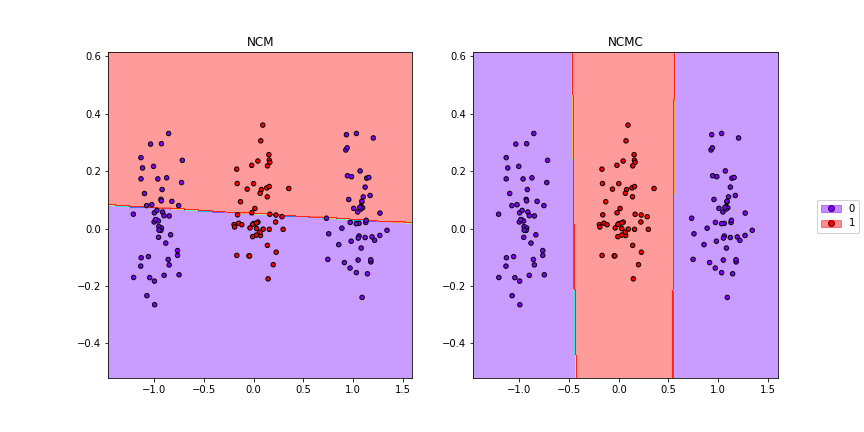
\includegraphics[width=1.0\textwidth]{images/ncm_problem.png}
    \caption{Conjunto de datos donde el clasificador NCM no da buenos resultados, pues los centroides de ambas clases son muy cercanos y ambos caen entre los puntos de la clase 1. Veremos que, escogiendo más de un centroide de forma adecuada podremos clasificar este conjunto como se muestra en la figura de la derecha.} \label{fig:problema_ncm}
\end{figure}

Una forma de solventar este problema es, en vez de considerar el centro de la clase para clasificar nuevos datos, encontrar subgrupos dentro de cada clase que presenten un agrupamiento de calidad, y para cada uno de estos subgrupos considerar su centro. Tendríamos de esta forma un conjunto de centroides para cada clase, y a la hora de clasificar un nuevo dato, bastaría seleccionar el centroide más cercano y asignarle la clase de la que es centroide.

Este nuevo clasificador, que denominaremos NCMC (\emph{Nearest Class Multiple Centroids}), entran en juego los algoritmos de segmentación o \emph{clustering}. Existen numerosos algoritmos \cite{clustering_algorithms} para obtener un conjunto de clusters dado un conjunto de datos, cada uno con sus ventajas e inconvenientes. Dada la forma de nuestro problema, en el que nos interesa además no solo obtener un conjunto de clusters para cada clase, sino además un centro para cada cluster, el algoritmo que reúne las condiciones más idóneas, además de ser sencillo y eficiente, es K-Means.

\subsubsection{K-Means y la búsqueda de centroides}

\emph{K-means} es uno de los algoritmos de \emph{clustering} más populares. La idea original de este algoritmo es, fijado un natural $k$, encontrar $k$ clusters, cada uno con un centroide, que minimicen una función de coste que depende de las distancias de los puntos del cluster a su centroide. Encontrar la solución a ese problema de optimización es un problema NP-hard, incluso para aproximarlo. En consecuencia, se utiliza comúnmente un algoritmo iterativo que garantiza la reducción de la función de coste en cada iteración, si bien los resultados que ofrece no son necesariamente los óptimos. Es por ello que normalmente se denomina K-means a este algoritmo iterativo, en lugar de a la minimización de la función objetivo asociada.

En primer lugar describimos la función objetivo. Consideramos el conjunto de datos $\mathcal{X} = \{x_1,\dots,x_N\} \subset \R^d$. La función objetivo dependerá de una familia de subconjuntos, $C_1,\dots,C_k$ que forman una partición de $\mathcal{X}$. A su vez, cada conjunto $C_i$ tendrá asociado un centroide $\mu_i$, que será aquel punto del espacio euclídeo $\mathbb{R}^d$ que minimice la suma de los cuadrados de las distancias de los elementos en $C_i$ a dicho centroide.  La función objetivo sumará los cuadrados de estas distancias para todos los clusters, quedando como se muestra a continuación:
\begin{equation} \label{eq:obj:kmeans}
    G(C_1,\dots,C_k) = \min_{\mu_1,\dots,\mu_k \in \R^d} \sum_{i=1}^{k}\sum_{x\in C_i} \|x-\mu_i\|^2.
\end{equation}

A continuación se describe el algoritmo iterativo que se utiliza normalmente para la búsqueda de los centroides. Inicialmente, se parte de unos centroides $\mu_1^{(0)},\dots,\mu_k^{(0)}$ escogidos al azar. En cada iteración $t$, se determina la partición $\{C_1^{(t)},\dots,C_k^{(t)}$ a partir de los centroides $\mu_1^{(t-1)},\dots,\mu_k^{(t-1)}$ de forma que a cada $x \in \mathcal{X}$ se le asigna el cluster del centroide más cercano. Finalmente, se calculan los nuevos centroides $\mu_1^{(t)},\dots,\mu_k^{(t)}$ como el vector media de los datos en $\{C_1^{(t)},\dots,C_k^{(t)}$, respectivamente. El proceso se repite hasta que en una iteración no se produzca ningún cambio en los clusters generados, momento en el que el algoritmo habrá convergido.

Como ya se ha mencionado, este algoritmo garantiza que la función objetivo \ref{eq:obj:kmeans} decrece conforme aumenta el número de iteraciones. A pesar de esto, no se puede asegurar que el algoritmo alcance un óptimo global (en ocasiones es posible incluso que ni siquiera se alcance un óptimo local). Sin embargo, el carácter aleatorio y la eficiencia del algoritmo permite realizar distintas ejecuciones eligiendo diferentes centroides iniciales, lo que facilita el encuentro de soluciones aceptables. 

Aunque se trata de un algoritmo eficiente y que en la práctica obtiene buenos resultados en la función objetivo, hay que destacar que es necesario especificar el número de clusters previamente. Los clusters que se obtienen con este algoritmo suelen tomar formas esféricas o similares, no siendo útiles para datos que presentan otros tipos de agrupaciones. También los datos más lejanos pueden condicionar en gran medida el valor de los centroides, y en consecuencia también el de los clusters.

Para la clasificación con NCMC, el uso de K-Means se reduce a aplicar el algoritmo de segmentación dentro de cada subconjunto de datos asociado a cada una de las clases del problema de clasificación. De esta forma obtenemos de forma sencilla el conjunto de centroides buscado para cada clase, y sobre el cual podemos realizar la clasificación de nuevos datos buscando simplemente el centroide más cercano. De nuevo se hace necesario establecer previamente el número de centroides para cada clase. Dichos números pueden estimarse realizando validación cruzada. 


\subsubsection{Aprendiendo distancias para NCMC}

Una vez definido el clasificador NCMC, el proceso de aprendizaje de distancias es análogo al de NCM. Siguiendo la notación utilizada en NCMML, en este caso, en lugar de un conjunto de centros de clase $\{\mu_c\}$, con $c \in \mathcal{C}$, disponemos de un conjunto de centroides, $\{m_{c_j}\}_{j=1}^{k_c}$, con $k_c \in \mathbb{N}$, para cada $c \in \mathcal{C}$. En este caso, las probabilidades asociadas a cada clase para la predicción correcta de $x \in \mathcal{X}$ vienen dadas por $p_L(c|x) = \sum_{j=1}^{k_c} p_L(m_{c_j}|x)$, donde son los centroides aquellos cuya probabilidad viene dada por la función softmax
\begin{equation}
    p_L(m_{c_j}|x) = \frac{\exp\left( -\frac{1}{2} \|L(x-m_{c_j})\|^2 \right)}{ \sum\limits_{c \in \mathcal{C}} \sum\limits_{i=1}^{k_c} \exp\left( -\frac{1}{2} \|L(x-m_{c_i})\|^2 \right) }.
\end{equation}

De nuevo, maximizamos el logaritmo de la verosimilitud, $\mathcal{L}(L) = \frac{1}{N}\sum_{i=1}^N p_L(y_i|x_i)$, cuyo gradiente en este caso viene dado por
\begin{equation*}
    \frac{\partial \mathcal{L}}{\partial L}(L) = \frac{1}{N} \sum_{i=1}^N \sum_{c \in \mathcal{C}} \sum_{j=1}^{k_c} \alpha_{ic_j} L (m_{c_j}-x_i)(m_{c_j}-x_i)^T,
\end{equation*}
donde $\alpha_{ic_j} = p_L(m_{c_j}|x_i) - [\![ y_i = c ]\!] \frac{p_L(m_{c_j}|x_i)}{\sum_{j'=1}^{k_c} p_L(m_{c_{j'}}|x_i)}$. La maximización de la verosimilitud por métodos de gradiente es la tarea llevada a cabo por la técnica de aprendizaje de distancias para NCMC, que denominaremos con el mismo nombre que dicho clasificador.





\section{Técnicas basadas en teoría de la información}

\subsection{ITML}

ITML (\emph{Information Theoretic Metric Learning}) \cite{itml} es una técnica de aprendizaje de métricas de distancia cuyo objetivo es encontrar una métrica lo más cercana posible a una distancia de partida, entendiendo la cercanía desde el punto de vista de la entropía relativa, como formularemos más adelante, haciendo que dicha métrica satisfaga determinadas restricciones de similitud para los datos entrenados.

ITML parte de un conjunto de datos $\mathcal{X} = \{x_1,\dots,x_N\} \subset \R^d$, no necesariamente etiquetados, pero del que se conoce que determinados pares de datos considerados similares deben estar a una distancia menor o igual que $u$, y otros pares de datos considerados no similares deben estar situados a una distancia mayor o igual que $l$, donde $u$ y $l$ son constantes prefijadas de antemano, con valores relativamente pequeño y grande, respectivamente, respecto al conjunto de datos.

A partir de los datos con las restricciones indicadas, ITML considera una métrica inicial asociada a una matriz $M_0$ definida positiva, y trata de encontrar una matriz definida positiva $M$, lo más parecida posible a $M_0$, y que respete las restricciones de similitud impuestas. La forma de medir el parecido entre $M$ y $M_0$ se realiza utilizando herramientas de la teoría de la información.

Es conocido que hay una correspondencia entre las matrices definidas positivas y las distribuciones normales multivariante, fijado un mismo vector media $\mu$. Dada $M \in \mathcal{M}_d(\R)^+$, podemos construir una distribución normal a través de su función de densidad,
\[ p(x;M) = \frac{1}{(2\pi)^{n/2}\det(M)^{1/2}}\exp\left( (x-\mu)^TM^{-1}(x-\mu) \right). \]
Recíprocamente, a partir de dicha distribución, si calculamos la matriz de covarianza recuperamos la matriz $M$. Usando esta correspondencia, vamos a medir la cercanía entre $M_0$ y $M$ a través de la divergencia KL entre sus correspondientes gaussianas,
\[ \kl(p(x;M_0))\|p(x;M)) = \int p(x;M_0)\log\frac{p(x;M_0)}{p(x;M)}dx. \]

Una vez definido el mecanismo con el que vamos a medir la cercanía de las métricas, podemos establecer la formulación del problema a optimizar por la técnica ITML. Si denominamos $S$ y $D$ a los conjuntos de pares de índices sobre los elementos de $\mathcal{X}$ que representan a los datos considerados similares y no similares, respectivamente, y partimos de la métrica inicial $M_0$, el problema es
\begin{equation} \label{eq:itml:prob1}
    \begin{split}
    \min_{M \succeq 0} &\quad \kl(p(x;M_0)\|p(x;M))  \\
    \text{s.a.: } &\quad d_M(x_i,x_j) \le u, \quad (i,j) \in S \\
                  &\quad d_M(x_i,x_j) \ge l, \quad (i,j) \in D.
    \end{split}
\end{equation}

Para tratar este problema computacionalmente, se hace uso de la divergencia matricial \emph{log-det}, la cual viene dada por
\[ D_{ld}(M\|M_0) = \tr(MM_0^{-1}) - \log\det(MM_0^{-1}) -d, \quad M,M_0 \in \mathcal{M}_d(\R)^+. \]

Hemos visto en el teorema \ref{prop:caract_kl:2} que la divergencia KL entre dos gaussianas con la misma media se puede expresar en términos de la divergencia \emph{log-det} como
\[ \kl(p(x;M_0)\|p(x;M)) = \frac{1}{2}D_{ld}(M_0\|M). \]

Esto nos permite reformular el problema \ref{eq:itml:prob1} de la siguiente forma:
\begin{equation} \label{eq:itml:prob2}
    \begin{split}
    \min_{M \succeq 0} &\quad D_{ld}(M_0\|M)  \\
    \text{s.a.: } &\quad \tr(M(x_i-x_j)(x_i-x_j)^T) \le u, \quad (i,j) \in S \\
                  &\quad \tr(M(x_i-x_j)(x_i-x_j)^T) \ge l, \quad (i,j) \in D.
    \end{split}
\end{equation}

Es posible que no se pueda encontrar una métrica que satisfaga simultáneamente todas las restricciones, por lo que el problema podría no tener solución. Por ello, ITML introduce en el problema \ref{eq:itml:prob2} variables de holgura mediante las cuales se obtiene un problema en cuya optimización se establece un equilibrio entre la minimización de la divergencia y la satisfacción de las restricciones, para poder llegar así a una solución aproximada del problema original, en caso de no tener solución. Finalmente, la técnica computacional utilizada en la resolución de este problema de optimización es la conocida como el método de las \emph{proyecciones de Bregman} \cite{bregman_projections}, el cual es una generalización del método de las proyecciones iteradas.
%% *** Completar cuando se haga el tema de teoría de la información.

\subsection{DMLMJ}

DMLMJ (\emph{Distance Metric Learning through the maximization of the Jeffrey divergence}) \cite{dmlmj} es una técnica de aprendizaje de métricas de distancia basada, al igual que ITML, en conceptos de teoría de la información. Concretamente, la herramienta que utiliza es la conocida como divergencia de Jeffrey, a través de la cual pretende separar lo máximo posible la distribución asociada a los puntos similares de aquella asociada a los puntos no similares, en los términos que veremos a continuación.

Consideramos el conjunto de entrenamiento $\mathcal{X} = \{x_1,\dots,x_N\} \subset \R^d$ con correspondientes etiquetas $y_1,\dots,y_N$, y fijamos $k \in \N, k \ge 1$. Como ya hemos comentado, DMLMJ busca maximizar, respecto a la divergencia de Jeffrey, la separación entre las distribuciones de puntos similares y no similares. Para ello, introduciremos los siguientes conceptos:

\begin{definition}
    Dado $x_i \in \mathcal{X}$, el \emph{vecindario $k$-positivo} de $x_i$ se define como el conjunto de los $k$ vecinos más cercanos de $x_i$ en $\mathcal{X} \setminus \{x_i\}$ cuya clase es la misma que la de $x_i$. Se nota por $V_k^+(x_i)$.

    El \emph{vecindario $k$-negativo} de $x_i$ se define como el conjunto de los $k$ vecinos más cercanos de $x_i$ en $\mathcal{X}$ cuya clase es distinta de la de $x_i$. Se nota por $V_k^-(x_i)$.

    Se define el \emph{espacio de diferencias $k$-positivo} del conjunto de datos etiquetados como el conjunto 
    \[ S = \{x_i - x_j \colon x_i \in \mathcal{X}, x_j \in V_k^+(x_i)\}. \]

    Análogamente, se define el \emph{espacio de diferencias $k$-negativo} como el conjunto
    \[ D = \{x_i - x_j \colon x_i \in \mathcal{X}, x_j \in V_k^-(x_i)\}. \]

\end{definition}

Los conjuntos $S$ y $D$ representan, por tanto, los vectores con las diferencias entre los datos y sus $k$ vecinos más cercanos, de igual o de distinta clase, respectivamente. Llamamos $P$ y $Q$ a las distribuciones en los espacios $S$ y $D$, respectivamente, asumiendo que son gaussianas multivariante. Asumiremos, además, que ambas distribuciones tienen media 0. Esta asunción es razonable, puesto que en la práctica, en la mayoría de los casos, si $x_i$ es vecino de $x_j$, $x_j$ también lo es de $x_i$, luego ambas diferencias aparecerán en el espacio de diferencias, haciendo la media cero. Por último, llamaremos a las correspondientes matrices de covarianza $\Sigma_S$ y $\Sigma_D$, respectivamente.

Si ahora aplicamos una transformación lineal a los datos, $x \mapsto Lx$, con $L \in \mathcal{M}_{d'\times d}(\R)$, las distribuciones transformadas seguirán teniendo media 0 y covarianzas $L\Sigma_S L^T$ y $L\Sigma_D L^T$, respectivamente. A dichas distribuciones las denominaremos $P_L$ y $Q_L$. El objetivo de DMLMJ es encontrar una transformación que maximice la divergencia de Jeffrey entre $P_L$ y $Q_L$:
\[ \max_{L \in \mathcal{M}_{d'\times d}(\R)} \quad f(L) =  \jf(P_L\|Q_L) = \kl(P_L\|Q_L) + \kl(Q_L\|P_L).\]

Como se demostró en la proposición \ref{prop:caract_jeffrey:2}, la divergencia de Jeffrey entre las distribuciones gaussianas $P_L$ y $Q_L$ se puede expresar como 
\[ f(L) = \frac{1}{2} \tr\left( (L\Sigma_S L^T)^{-1} (L\Sigma_D L^T) + (L \Sigma_D L^T)^{-1} (L \Sigma_S L^T) \right) - d'. \]

Como $d'$ es constante, obtenemos el problema equivalente
\[ \max_{L \in \mathcal{M}_{d'\times d}(\R)} \quad J(L) =  \tr\left( (L\Sigma_S L^T)^{-1} (L\Sigma_D L^T) + (L \Sigma_D L^T)^{-1} (L \Sigma_S L^T) \right).\]

Si calculamos el gradiente de la función anterior, obtenemos
\[ \nabla J(L) = \left( 2 \Sigma_D L^T\Sigma_{2S}^{-1} - 2\Sigma_S L^T \Sigma_{2S}^{-1}\Sigma_{2D}\Sigma_{2S}^{-1} \right) + \left( 2\Sigma_S L^T \Sigma_{2D}^{-1} - 2 \Sigma_D L^T \Sigma_{2D}^{-1}\Sigma_{2S} \Sigma_{2D}^{-1} \right),\]
donde $\Sigma_{2S} = L \Sigma_S L^T$ y $\Sigma_{2D} = L\Sigma_D L^T$.

Cada uno de los términos entre paréntesis se anula, respectivamente, cuando $\Sigma_S^{-1} \Sigma_D L^T = L^T \Sigma_{2S}^{-1} \Sigma_{2D}$ y cuando $\Sigma_{D}^{-1}\Sigma_S L^T = L^T \Sigma_{2D}^{-1} \Sigma_{2S}$. Queremos resolver estas dos ecuaciones. Para ello, enunciamos los siguientes resultados.

\begin{thm}

    Sean $\Sigma_1, \Sigma_2 \in \mathcal{M}_d(\R)^+$ y sea $L \in \mathcal{M}_{d'\times d}(\R)$ una matriz que contiene, por filas, $d'$ vectores propios linealmente independientes de $\Sigma_1^{-1}\Sigma_2$. Entonces,
    \begin{equation} \label{eq:jef:thm1}
        \Sigma_1^{-1}\Sigma_2L^T = L^T(L\Sigma_1L^T)^{-1}(L\Sigma_2L^T).
    \end{equation}
\end{thm}

\begin{proof} \label{thm:dmlmj1}
    Sea $D \in \mathcal{M}_{d'}(\R)$ la matriz diagonal que contiene, en el mismo orden, los $d'$ valores propios de $\Sigma_1^{-1}\Sigma_2$ asociados a los vectores propios presentes en $L$. Se verifica entonces
    \begin{equation}\label{eq:jef:formula_vp}
        \Sigma_1^{-1}\Sigma_2L^T = L^TD.
    \end{equation} 

    Si multplicamos a ambos lados por $L\Sigma_1$, obtenemos
    \[ L\Sigma_2L^T = L\Sigma_1L^TD. \]

    $L\Sigma_1L^T$ es una matriz regular. Puesto que $\Sigma_1$ es definida positiva, admite una descomposición $\Sigma_1 = PP^T$, con $P$ regular de dimensión $d$. Entonces, $L\Sigma_1L^T = LPP^TL^T = LP(LP)^T$, donde $LP$ es una matriz cuadrada de dimensión $d'$ y de rango $d'$, por ser la composición (viéndolas como aplicaciones lineales) de un isomorfismo con una aplicación de rango $d'$, haciendo que la imagen tenga de nuevo dimensión $d'$. En consecuencia, $LP$ es regular, y por tanto también lo es $LP(LP)^T = L\Sigma_1L^T$, por lo que podemos tomar inversas, obteniendo
    \begin{equation} \label{eq:jef:coro1_pre}
        (L\Sigma_1L^T)^{-1}(L\Sigma_2L^T) = D.
    \end{equation}

    Si a continuación multiplicamos a la izquierda por $L^T$ en ambos lados de la igualdad, se tiene
    \[ L^T(L\Sigma_1L^T)^{-1}(L\Sigma_2L^T) = L^TD. \]

    Sustituyendo lo que acabamos de obtener en el lado derecho de \ref{eq:jef:formula_vp}, concluimos que
    \[\Sigma_1^{-1}\Sigma_2L^T = L^T(L\Sigma_1L^T)^{-1}(L\Sigma_2L^T).\]

\end{proof}

\begin{cor} \label{cor:dmlmj1}
    Sean $\Sigma_1, \Sigma_2 \in \mathcal{M}_d(\R)^+$ y sea $L \in \mathcal{M}_{d'\times d}(\R)$ una matriz que contiene, por filas, $d'$ vectores propios linealmente independientes de $\Sigma_1^{-1}\Sigma_2$. Sea $D \in \mathcal{M}_{d'}(\R)$ la matriz diagonal con los correspondientes $d'$ valores propios. Entonces,
    \[ \tr\left( (L\Sigma_1L^T)^{-1}(L\Sigma_2L^T) \right) = \tr(D). \]
\end{cor}

\begin{proof}
    Basta tomar trazas en la igualdad de matrices de la ecuación \ref{eq:jef:coro1_pre}.
    \begin{comment}
    Se verifica de nuevo la ecuación \ref{eq:jef:formula_vp}. Combinándola con la ecuación \ref{eq:jef:thm1} del teorema anterior, se tiene
    \[ L^T(L\Sigma_1L^T)^{-1}(L\Sigma_2L^T) = L^TD. \]

    $L^T$ es una matriz de dimensión $d\times d'$, con $d' \le d$ y de rango máximo, luego admite una inversa por la izquierda. Multiplicando por dicha inversa, obtenemos
    \[ (L\Sigma_1L^T)^{-1}(L\Sigma_2L^T) = D.\]

    La prueba concluye al tomar trazas en esta última igualdad de matrices.
    \end{comment}
\end{proof}

De acuerdo con el teorema \ref{thm:dmlmj1}, podemos observar que es posible anular simultáneamente ambos términos del gradiente tomando $L$ como una matriz de vectores propios de $\Sigma_S^{-1}\Sigma_D$, o bien de $\Sigma_D^{-1}\Sigma_S$. Notemos que ambos casos comparten los mismos vectores propios y cada opción tiene como valores propios los inversos de la opción restante. Optamos por tomar $d'$ vectores propios del primer caso, de $\Sigma_S^{-1}\Sigma_D$. Entonces, $\nabla J(L) = 0$ y el corolario \ref{cor:dmlmj1} nos dice que
\begin{align*}
    J(L) &= \tr\left( (L\Sigma_S L^T)^{-1} (L\Sigma_D L^T) + (L \Sigma_D L^T)^{-1} (L \Sigma_S L^T) \right) \\
         &= \tr\left( (L\Sigma_S L^T)^{-1} (L\Sigma_D L^T)\right) + \tr\left((L \Sigma_D L^T)^{-1} (L \Sigma_S L^T) \right) \\
         &= \tr\left(\Lambda\right) + \tr\left(\Lambda^{-1}\right) = \sum\limits_{i=1}^{d'} \left( \lambda_i + \frac{1}{\lambda_i} \right),
\end{align*}

donde $\Lambda = \diag(\lambda_1,\dots,\lambda_{d'})$ es la matriz diagonal con los valores propios asociados a los vectores propios escogidos de $\Sigma_S^{-1}\Sigma_D$.

Por tanto, para maximizar $J(L)$ debemos seleccionar los $d'$ vectores propios asociados a los $d'$ valores propios $\lambda$ para los cuales sea mayor la expresión $\lambda + 1/\lambda$. La transformación $L$ construida a partir de dichos vectores propios determina la distancia que es aprendida mediante la técnica DMLMJ.

Finalmente, el único requerimiento adicional necesario para completar esta construcción es el cálculo de las matrices de covarianza. Teniendo en cuenta que se ha asumido que la media de las distribuciones es 0, podemos obtener dichas matrices de forma sencilla a partir de los vectores de diferencias, como se muestra a continuación.
\begin{equation*}
    \Sigma_S = \frac{1}{|S|}\sum_{i=1}^{N} \left[ \sum_{x_j \in V_k^+(x_i)} (x_i-x_j)(x_i-x_j)^T\right], \quad \Sigma_D = \frac{1}{|D|}\sum_{i=1}^{N} \left[ \sum_{x_j \in V_k^-(x_i)} (x_i-x_j)(x_i-x_j)^T\right].
\end{equation*}

%% (usando estimacion de maxima verosimilitud ????) ***
%% Comentario final ***

\subsection{MCML}

MCML (\emph{Maximally Collapsing Metric Learning}) \cite{mcml} es una técnica de aprendizaje de métricas de distancia supervisado, que se basa en la idea de que si todos los datos de una misma clase fueran proyectados a un mismo punto, y los datos de distintas clases fueran proyectados en puntos distintos y suficientemente alejados, tendríamos, sobre los datos proyectados, una separación de clases ideal.  Su finalidad es aprender una métrica de distancia que permita colapsar lo máximo posible, dentro de las limitaciones de la métrica, todos los datos de una misma clase en un único punto, arbitrariamente alejado de los puntos en los que colapsarán los datos del resto de las clases.

Consideramos el conjunto de datos $\mathcal{X} = \{x_1,\dots,x_N\} \subset \R^d$, con etiquetas asociadas $y_1,\dots,y_N$. Queremos aprender una métrica determinada por una matriz $M \succeq 0$ que trate de colapsar al máximo las clases según el enfoque del párrafo anterior. La forma de abordar este problema va a consistir una vez más en utilizar las herramientas proporcionadas por la teoría de la información. Para ello, en primer lugar, introducimos una distribución condicionada sobre los puntos del conjunto de datos en forma de \emph{softmax}, análoga a la establecida en el caso de NCA. Si $i,j \in \{1,\dots,N\}$ con $i \ne j$, definimos la probabilidad de que $x_j$ sea clasificado con la clase de $x_i$ según la distancia entre $x_i$ y $x_j$ que determina $M$ como
\begin{equation}
    p^{M}(j|i) = \frac{\exp(-\|x_i-x_j\|^2_M)}{\sum\limits_{k\ne i} \exp(-\|x_i-x_k\|^2_M)}.
\end{equation}

Por otra parte, la distribución ideal que buscamos obtener es una distribución binaria para la que la probabilidad de que a un dato se le asigne su clase correcta es 1, y 0 en caso contrario, es decir,
\begin{equation}
    p_0(j|i) \propto \begin{cases}1, &\quad y_i = y_j \\ 0, &\quad y_i \ne y_j\end{cases}.
\end{equation}

Notemos que durante el entrenamiento conocemos las clases reales de los datos, luego podemos tratar esta última probabilidad. Además, observemos que si conseguimos una métrica $M$ cuyas distribuciones $p^M$ asociadas coincidan con $p_0$, entonces, bajo unas mínimas condiciones de suficiencia de datos, estaremos consiguiendo colapsar las clases en puntos infinitamente alejados. 

En efecto, supongamos que hay al menos $r + 2$ datos en cada clase, donde $r$ es el rango de $M$, y que $p^M(j|i) = p_0(j|i)$ para cualesquiera $i,j \in \{1,\dots,N\}$. Entonces, por un lado, de $p^M(j|i) = 0$ para $y_i \ne y_j$ se deduce que $\exp(-\|x_i-x_j\|^2_M) = 0$, lo que conduce indudablemente a que $x_i$ y $x_j$ estén infinitamente alejados cuando sus clases son distintas. Por otra parte, de $p^M(j|i) \propto 1$ para cualesquiera $x_i,x_j$ con $y_i = y_j$ se deduce que el valor $\exp(\|x_i-x_j\|_M^2)$ es constante para todos los miembros de una misma clase, y en consecuencia todos los puntos en una misma clase son equidistantes. Como $M$ tiene rango $r$ está induciendo una distancia sobre un subespacio de dimensión $r$, donde se sabe que a lo sumo puede haber $r+1$ puntos distintos y equidistantes entre sí (esto se debe a que los puntos distintos equidistantes para una distancia procedente de un producto escalar han de ser afinmente independientes). Como estamos asumiendo que hay al menos $r+2$ puntos por clase, todos los puntos de la misma clase han de tener distancia 0 entre sí respecto a $M$, colapsando por tanto en un único punto.

Una vez establecidas ambas distribuciones, el objetivo de MCML es, como ya hemos comentado, aproximar $p^M(\cdot|i)$ a $p_0(\cdot|i)$ lo máximo posible, para cada $i$ utilizando para ello la entropía relativa entre ambas distribuciones. El problema de optimización consiste, por tanto, en minimizar esta divergencia,
\begin{equation}
    \min_{M \succeq 0}\quad f(M) = \sum_{i=1}^N \kl \left[ p_0(j|i) \| p^M(j|i) \right].
\end{equation} 

Podemos reescribir la función objetivo en términos de funciones más elementales.
\begin{equation} \label{eq:mcml:fobj2}
    \begin{split}
        f(M) &= \sum_{i=1}^N \sum_{j=1}^N p_0(j|i) \log \frac{p_0(j|i)}{p^M(j|i)} = \sum_{i=1}^N \sum_{j \colon y_i = y_j}\log\frac{1}{p^M(j|i)} \\
             &= \sum_{i=1}^N \sum_{j \colon y_i = y_j}-\log p^M(j|i) = - \sum_{i=1}^N \sum_{j \colon y_i = y_j}\left(-\|x_i-x_j\|_M^2-\log\sum_{k \ne i} \exp(-\|x_i-x_k\|^2)\right)\\
             &= \sum_{i=1}^N \sum_{j \colon y_i = y_j}\|x_i-x_j\|_M^2+\sum_{i=1}^N\log\sum_{k \ne i} \exp(-\|x_i-x_k\|^2).
    \end{split}
\end{equation}

Cada sumando de la expresión anterior es convexo en $M$, el primero por tratarse de una función distancia en $M$ (que es lineal), y el segundo por tratarse de una función logaritmo de suma de exponenciales (convexo) compuesto con una función distancia. Además, la restricción $M \succeq 0$ también es convexa, luego el problema a optimizar es convexo. La función objetivo es siempre no negativa, pues $\|x_i-x_j\|_M^2\ge - \log\sum_{k \ne i} \exp(-\|x_i-x_k\|^2)$, pues el lado derecho de la desigualdad siempre contiene al menos una exponencial con el término $-\|x_i-x_j\|_M^2$ y el logaritmo es creciente. Luego el problema es convexo y minorado, lo que nos garantiza que se alcanza un mínimo global y no hay mínimos locales. Podemos por tanto encontrar dicho óptimo utilizando los mecanismos de la optimización convexa.

Concretamente, la técnica de optimización propuesta en MCML es la ya comentada programación semidefinida. Para ello, es necesario una expresión del gradiente de la función objetivo, el cual puede ser calculado a partir de su expresión en \ref{eq:mcml:fobj2}:
\begin{equation*}
    \nabla f(M) = \sum_{i,j\colon y_i = y_j}(x_i - x_j)^T(x_i-x_j) - \sum_i \frac{-\sum\limits_{k \ne i} (x_i-x_k)^T(x_i-x_k) \exp(-\|x_i-x_k\|_M^2)}{ \sum\limits_{k \ne i} \exp(-\|x_i-x_k\|^2_M)}.
\end{equation*}

La minimización de la función objetivo \ref{eq:mcml:fobj2} de forma iterativa mediante descensos en la dirección del gradiente combinado con proyecciones sobre el cono de las matrices semidefinidas positivas es la tarea llevada a cabo por el algoritmo MCML.

\section{Otras técnicas de aprendizaje de métricas de distancia}

\subsection{LSI} \label{lsi}

LSI (\emph{Learning with Side Information}) \cite{lsi}, también denominado a veces MMC (\emph{Mahalanobis Metric for Clustering}) es una técnica de aprendizaje de métricas de distancia que trabaja con un conjunto de datos, no necesariamente etiquetados, sobre los que se conoce, como información adicional, determinadas parejas de puntos que se sabe que son similares y, opcionalmente, parejas de puntos que se sabe que no lo son.

LSI trata de aprender una métrica $M$ que respete esta información adicional. Es por ello que puede ser utilizado tanto en aprendizaje supervisado, donde los pares similares corresponderán a datos con la misma etiqueta, como en aprendizaje no supervisado con restricciones de similaridad, como por ejemplo, problemas de clustering donde se conoce que determinados datos deben ser agrupados en el mismo cluster.

Pasamos a formular el problema a optimizar. Supongamos que nuestro conjunto de datos es $\mathcal{X} = \{x_1,\dots,x_N\} \subset \R^d$ y conocemos adicionalmente el conjunto $S = \{(x_i,x_j) \in \mathcal{X}\times\mathcal{X} \colon x_i \textit{ y } x_j \textit{ son similares.}\}$. De forma adicional, podemos conocer el conjunto $D = \{(x_i,x_j) \in \mathcal{X}\times\mathcal{X} \colon x_i \textit{ y } x_j \textit{ no son similares.} \}$. En caso de no disponer de este último, podemos tomar $D$ como el complemento de $S$ en $\mathcal{X} \times \mathcal{X}$.

La primera intuición para abordar este problema, dada la información de la que disponemos, es minimizar las distancias entre los pares de puntos similares, esto es, minimizar $\sum_{(x_i,x_j)\in S} \|x_i - x_j \|_M^2$, donde $(x_i - x_j)^T M (x_i - x_j)$ y $M \in \mathcal{M}_{d}(\R)^+_0$. Sin embargo, esto nos conduce a la solución $M = 0$, lo cual no nos aportaría ninguna información productiva. Por eso, LSI añade la restricción adicional $\sum_{(x_i,x_j) \in D} \|x_i - x_j\|_M \ge 1$, lo que nos conduce al problema de optimización
\begin{equation} \label{eq:lsi}
\begin{split}
    \min_{M} &\quad \sum_{(x_i,x_j)\in S}  \|x_i - x_j \|_M^2 \\
    \text{s.a.: } &\quad \sum_{(x_i,x_j) \in D} \|x_i - x_j\|_M \ge 1 \\
                  &\quad M \succeq 0.
\end{split}
\end{equation}

Notemos varias observaciones respecto a esta fórmula. En primer lugar, la elección de la constante 1 en la restricción es irrelevante; si escogemos cualquier constante $c > 0$ obtenemos una métrica proporcional a $M$. Por otra parte, el problema de optimización es convexo, pues los conjuntos determinados por las restricciones son convexos y la función a optimizar también lo es. Por último, podríamos plantearnos una restricción sobre el conjunto $D$ de la forma $\sum_{(x_i,x_j) \in D} \|x_i - x_j\|_M^2 \ge 1$. Sin embargo, un razonamiento similar al utilizado en LDA permite probar que en tal caso la métrica aprendida va a tener rango 1, lo cual puede no resultar óptimo.

Para la resolución de este problema los autores proponen el problema equivalente
\begin{equation} \label{eq:lsi:equiv}
\begin{split}
    \max_{M} &\quad \sum_{(x_i,x_j)\in D}  \|x_i - x_j \|_M \\
    \text{s.a.: } &\quad \sum_{(x_i,x_j) \in S} \|x_i - x_j\|_M^2 \le 1 \\
                  &\quad M \succeq 0.
\end{split}
\end{equation}
Este problema con dos restricciones convexas puede ser resuelto mediante métodos de gradiente ascendente combinados con proyecciones que satisfagan las restricciones del problema. En este problema, las restricciones son fáciles de satisfacer por separado. La primera restricción consiste en una proyección sobre un semiespacio afín, mientras que la segunda consiste en una proyección sobre el cono de matrices semidefinidas positivas. El método de las proyecciones iteradas justificado por el teorema \ref{thm:iter_proj} permite satisfacer ambas restricciones proyectando repetidas veces sobre ambos conjuntos, hasta obtener la convergencia.

\subsection{DML-eig}

DML (\emph{Distance Metric Learning with Eigenvalue Optimization}) \cite{dmleig} es una técnica de aprendizaje de métricas de distancia inspirada en la técnica LSI de la sección anterior, proponiendo un problema de optimización muy similar pero ofreciendo un método de resolución completamente diferente, basado en la optimización de valores propios.

Consideramos, al igual que en el caso anterior, un conjunto de datos de entrenamiento $\mathcal{X} = \{x_1,\dots,x_N\} \subset \R^d$, del que conocemos dos subconjuntos $S$ y $D$ de $\mathcal{X}\times\mathcal{X}$ de datos considerados similares, y no similares, respectivamente. En la sección anterior, para optimizar el problema \ref{eq:lsi:equiv} se proponía un método de gradiente ascendente con proyecciones iteradas, el cual puede requerir bastante tiempo para converger. La propuesta de DML-eig consiste en una ligera modificación de la función objetivo, manteniendo las restricciones, que nos conduce al problema
\begin{equation} \label{eq:dmleig:1}
\begin{split}
    \max_{M} &\quad \min_{(x_i,x_j)\in D}  \|x_i - x_j \|_M^2 \\
    \text{s.a.: } &\quad \sum_{(x_i,x_j) \in S} \|x_i - x_j\|_M^2 \le 1 \\
                  &\quad M \succeq 0.
\end{split}
\end{equation}

Para abordar la resolución de este problema resulta útil introducir una notación que simplifique la indexación de los datos. En primer lugar, denotaremos $X_{ij} = (x_i-x_j)(x_i-x_j)^T$ a los productos tensoriales entre las diferencias de elementos de $\mathcal{X}$. Para acceder a pares de elementos $(i,j)$ utilizaremos un único índice $\tau \equiv (i,j)$. Dicho índice lo podremos suponer ordenado cuando sea necesario para acceder a las distintas componentes de un vector de dimensión adecuada. Al producto tensorial anterior $X_{ij}$ también lo podremos notar como $X_{\tau}$. Por último, los conjuntos $S$ y $D$ también supondremos que están formados por índices $\tau$ asociados a un par $(i,j)$ tales que $x_i$ y $x_j$ son similares o no similares, respectivamente. De esta forma, si denotamos $X_S = \sum_{(i,j)\in S}X_{ij}$, el problema \ref{eq:dmleig:1} podemos reescribirlo en términos del producto escalar de Frobenius como
\begin{equation} \label{eq:dmleig:2}
\begin{split}
    \max_{M} &\quad \min_{\tau \in D}  \langle X_{\tau}, M \rangle \\
    \text{s.a.: } &\quad \langle X_S, M \rangle \le 1 \\
                  &\quad M \succeq 0.
\end{split}
\end{equation}

Veamos cómo se establece la formulación del problema que buscamos en términos de optimización de valores propios. Para cada matriz simétrica $X \in S_d(\R)$ denotamos a su mayor valor propio como $\lambda_{\max}(X)$. Asociado al conjunto $D$ de pares no similares vamos a definir el simplex
\[ \Delta = \left\{u \in \R^{|D|} \colon u_\tau \ge 0 \ \forall \tau \in D, \sum_{\tau \in D} u_{\tau} = 1 \right\}. \]
También consideramos el conjunto
\[ \mathcal{P} = \{M \in \mathcal{M}_d(\R)^+_0 \colon \tr(M) = 1 \}.  \]
$\mathcal{P}$ es la intersección del cono de matrices semidefinidas positivas con un subespacio afín de $\mathcal{M}_d(\R)$. A los conjuntos que presentan esta estructura se les conoce como \emph{espectraedros}. 

Entonces, si $X_S$ es definida positiva y definimos, para cada $\tau \in D$, $\widetilde{X}_{\tau} = X_S^{-1/2}X_{\tau}X_S^{-1/2}$, se puede probar \cite{dmleig} que el problema \ref{eq:dmleig:2} es equivalente al siguiente problema
  \begin{equation} \label{eq:dmleig:3}
      \max_{S \in \mathcal{P}} \min_{u \in \Delta} \sum_{\tau \in D} u_{\tau}\langle \widetilde{X}_{\tau},S\rangle,
  \end{equation}
  el cual se puede reescribir a su vez como un problema de optimización de valores propios:
  \begin{equation} \label{eq:dmleig:4}
      \min_{u \in \Delta} \max_{S \in \mathcal{P}} \left\langle \sum_{\tau \in D} u_{\tau} \widetilde{X}_{\tau},S\right\rangle = \min_{u \in \Delta} \lambda_{\max}\left( \sum_{\tau\in D}u_{\tau}\widetilde{X}_{\tau} \right).
  \end{equation}

\begin{comment}
\begin{thm}
    Supongamos que $X_S$ es definida positiva y definimos, para cada $\tau \in D$, definimos $\widetilde{X}_{\tau} = X_S^{-1/2}X_{\tau}X_S^{-1/2}$. Entonces, el problema \ref{eq:dmleig:2} es equivalente al siguiente problema
    \begin{equation} \label{eq:dmleig:3}
        \max_{S \in \mathcal{P}} \min_{u \in \Delta} \sum_{\tau \in D} u_{\tau}\langle \widetilde{X}_{\tau},S\rangle,
    \end{equation}
    el cual se puede reescribir a su vez como un problema de optimización de valores propios:
    \begin{equation} \label{eq:dmleig:4}
        \min_{u \in \Delta} \max_{S \in \mathcal{P}} \left\langle \sum_{\tau \in D} u_{\tau} \widetilde{X}_{\tau},S\right\rangle = \min_{u \in \Delta} \lambda_{\max}\left( \sum_{\tau\in D}u_{\tau}\widetilde{X}_{\tau} \right).
    \end{equation}
\end{thm}

\begin{proof}

\end{proof}
\end{comment}

El problema de minimizar el mayor valor propio de una matriz simétrica es conocido y se conocen algoritmos iterativos que permiten alcanzar dicho mínimo \cite{overton1988minimizing}. Además, en \cite{dmleig} se propone un algoritmo para resolver el problema $\max_{S \in \mathcal{P}} \min_{u \in \Delta} \sum_{\tau \in D} u_{\tau}\langle \widetilde{X}_{\tau},S\rangle + \mu \sum_{\tau \in D} u_{\tau} \log u_{\tau}$, donde $\mu > 0$ es un parámetro de suavizado, mediante el cual se puede aproximar el problema \ref{eq:dmleig:4}.

%% Terminar con matemáticas.




\subsection{LDML}

LDML (\emph{Logistic Discriminant Metric Learning}) \cite{ldml} es una técnica de aprendizaje de métricas de distancia en cuyo modelo de optimización se hace uso de la función logística. Los autores afirman que esta técnica es bastante útil para aprender distancias sobre conjuntos de imágenes etiquetadas, pudiendo utilizarse por tanto en problemas como la identificación de caras.

Recordamos que la función sigmoide es la aplicación $\sigma\colon \R \to \R$ dada por
\[ \sigma(x) = \frac{1}{1+e^{-x}}. \]

Esta función presenta una gráfica con una forma sigmoidal, es diferenciable, estrictamente creciente y toma valores entre 0 y 1, alcanzando dichos valores en sus límites en menos infinito y más infinito, respectivamente. Estas propiedades permiten que la función logística sea la función de distribución de una variable aleatoria, lo que le da una importante utilidad probabilística. Su gráfica presenta  un comportamiento asintótico a partir de valores pequeños (en valor absoluto), con un crecimiento exponencial en zonas cercanas al cero. Esto hace que sea de gran utilidad para modelar señales binarias. También presenta una derivada fácil de calcular, y expresable en términos de la propia función logística, $\sigma'(x) = \sigma(x)(1-\sigma(x))$. En la Figura \ref{fig:funcion_logistica} se muestra la gráfica de esta función. La función logística es también de gran utilidad en otras ramas del aprendizaje automático, como es el caso de la regresión logística o de las redes neuronales.

\begin{figure}[h]
    \centering
    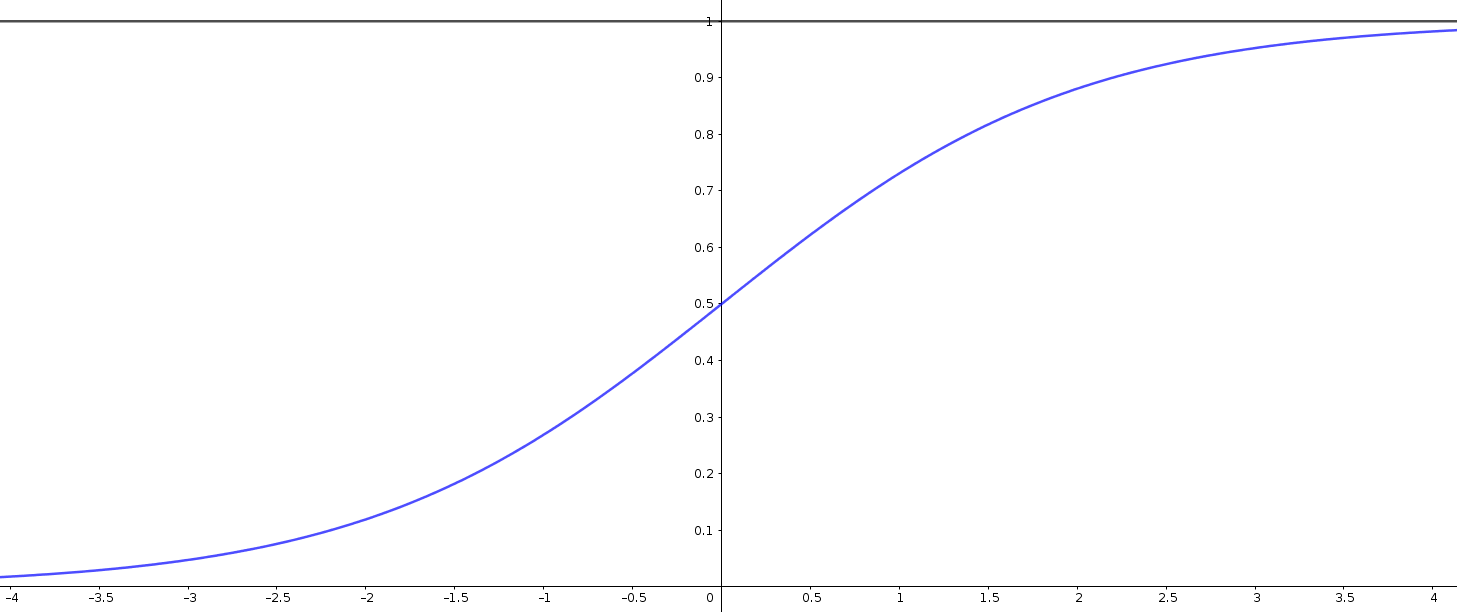
\includegraphics[width=0.65\textwidth]{images/logistica.png}
    \caption{La función logística.} \label{fig:funcion_logistica}
\end{figure}

Supongamos el conjunto de datos $\mathcal{X} = \{x_1,\dots,x_N\} \subset \R^d$, con correspondientes etiquetas $y_1,\dots,y_N$. En LDML, la función logística se utiliza para definir una probabilidad, la cual asignará a pares de puntos una probabilidad mayor conforme menor sea la distancia entre ellos. Para medir la distancia, LDML utilizará una matriz de métrica $M$ semidefinida positiva, quedando la expresión de la probabilidad como
\begin{equation}
    p_{ij,M} = \sigma(b - \|x_i-x_j\|_M^2),
\end{equation} 

donde $b$ es un valor umbral positivo que determinará el valor máximo alcanzable por la función logística, y que puede ser estimado mediante validación cruzada. Asociada a esta probabilidad podemos definir una variable aleatoria que sigue una distribución de Bernouilli, y que toma los valores 0 y 1, según el par $(x_i,x_j)$ pertenezca o no a la misma clase. Dicha distribución viene determinada por la función masa de probabilidad
\[ f_{ij,M}(x) = (p_{ij,M})^{x}(1-p_{ij,M})^{1-x}, \quad x  \in \{0,1\}. \]

La función que busca maximizar la técnica LDML es el logaritmo de la verosimilitud de la distribución anterior para el conjunto de datos dado, esto es,
\begin{equation}
    \mathcal{L}(M) = \sum_{i,j=1}^N y_{ij}\log p_{ij,M} + (1-y_{ij})\log(1-p_{ij,M}),
\end{equation}

donde $y_{ij}$ es una variable binaria que toma el valor 1 si $y_i = y_j$, y 0 en caso contrario. Esta función es diferenciable, cóncava (es una combinación positiva de funciones que se pueden expresar como un menos logaritmo de suma de exponenciales, que son cóncavos) y está mayorada, luego tenemos la garantía de poder alcanzar un máximo global. Teniendo en cuenta que, si $x_{ij} \equiv (x_i-x_j)^T(x_i-x_j)$ y $p_{ij} \equiv p_{ij,M}$, y por las propiedades de la derivada de la función logística su gradiente presenta la expresión
\begin{align*}
    \mathcal{\nabla L}(M) &= \sum_{i,j=1}^N y_{ij}\frac{-x_{ij} p_{ij}(1 - p_{ij})}{p_{ij}} + (1-y_{ij})\frac{x_{ij}p_{ij}(1-p_{ij})}{1-p_{ij}} \\
                          &= \sum_{i,j=1}^N -y_{ij}x_{ij}(1 - p_{ij}) + (1-y_{ij})x_{ij}p_{ij} \\
                          &= \sum_{i,j=1}^N x_{ij}((1-y_{ij})p_{ij}-(1-p_{ij})y_{ij}) \\
                          &= \sum_{i,j=1}^N x_{ij}(p_{ij}-y_{ij}),
\end{align*}

los métodos iterativos de gradiente ascendente combinados con proyecciones sobre el cono de las matrices semidefinidas positivas, conforman el algoritmo de programación semidefinida que es utilizado en LDML para la obtención de la métrica que optimiza su función objetivo.

%% *** Imagen de la funcion logistica



\section{El kernel trick. Algoritmos de aprendizaje de métricas de distancia basados en kernels}

\subsection{El kernel trick}

Los métodos de kernel conforman un paradigma dentro del aprendizaje automático que resulta de gran utilidad en muchos de los problemas que se abordan en esta disciplina. Normalmente surgen en problemas en los que el algoritmo de aprendizaje ve mermada su capacidad, generalmente, debido a la forma del conjunto de datos. Esto ocurre, por ejemplo, en las máquinas de vectores soporte. Aunque no vamos a entrar en los detalles de este algoritmo, nos va a servir para ilustrar la necesidad de los métodos de kernel en el aprendizaje automático.

Las \emph{máquinas de vectores soporte} (SVM, \emph{Support Vector Machines}) son un modelo de clasificación lineal binario que, en su versión más sencilla, cuando los datos son separables, busca establecer el hiperplano que mejor que mejor separa los datos, esto es, aquel para el cual se maximiza la distancia (margen) a los conjuntos que determinan cada clase. Los puntos de ambos conjuntos donde se materializa dicho margen son los denominados \emph{vectores soporte}. En la Figura \ref{fig:svm_ejemplo} se muestra cómo actúa este clasificador.

\begin{figure}[h]
    \centering
    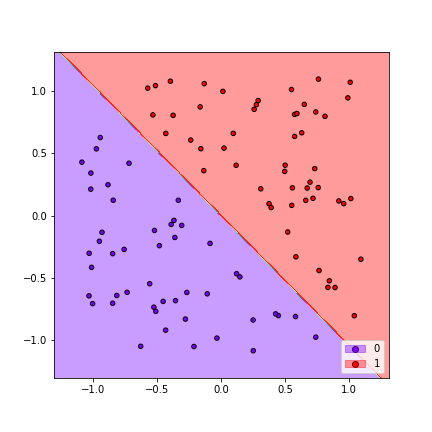
\includegraphics[width=0.5\textwidth]{images/svm_example.png}
    \caption{Clasificación realizada por las máquinas de vectores soporte en su versión básica.} \label{fig:svm_ejemplo}
\end{figure} 

Sin embargo, en muchas ocasiones, aunque los datos sean visiblemente separables, puede resultar imposible separarlos mediante un hiperplano, como sucede en el ejemplo de la Figura \ref{fig:svm_ejemplo2}. En ella, se ha considerado un subconjunto finito $\mathcal{X}$ de números reales, de forma que a aquellos $x \in \mathcal{X}$ con $|x| > 1$ se les ha asignado la clase $1$ y a aquellos con $|x| \le 1$ la clase $-1$. Es inmediato observar que, aunque las regiones de las dos clases están claramente diferenciadas, no es posible separarlas mediante un hiperplano.

\begin{figure}[h]
    \centering
    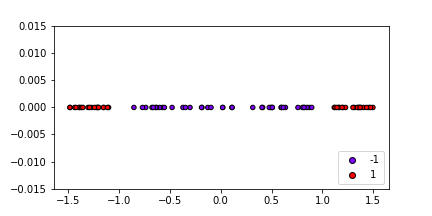
\includegraphics[width=0.5\textwidth]{images/svm_problem.png}
    \caption{Conjunto de datos para el que SVM no puede establecer un hiperplano separador.} \label{fig:svm_ejemplo2}
\end{figure} 

A pesar de esto, es posible establecer una transformación en los datos que los incluya en un espacio de dimensión mayor en el cual los datos sí sean separables mediante hiperplanos. En efecto, si definimos la aplicación $\phi\colon \R \to \R^2$ por $\phi(x) = (x,x^2)$, los datos de $\phi(\mathcal{X})$ sí que son separables en $\R^2$. Concretamente, podemos tomar el hiperplano $H = \{(x,y) \in \R^2 \colon y = 1\}$ como hiperplano separador. Esta misma idea podemos utilizarla sobre SVM: transformamos los datos y aplicamos el algoritmo en el espacio transformado obteniendo el hiperplano. Si después queremos predecir la clase de un nuevo dato, podemos aplicarle la transformación y asignarle la clase según el lado del hiperplano en el que ha caído. La Figura \ref{fig:svm_ejemplo3} muestra el resultado de aplicar SVM en el espacio transformado sobre el ejemplo dado.

\begin{figure}[h]
    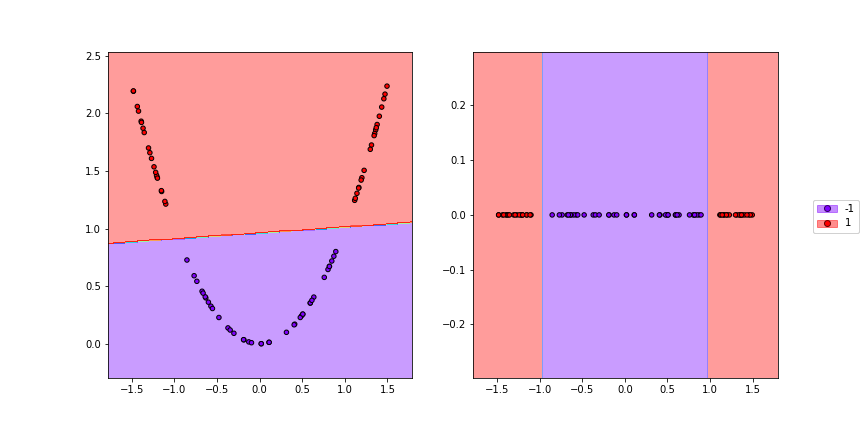
\includegraphics[width=0.8\textwidth]{images/svm_solution.png}
    \centering
    \caption{Resolución mediante máquinas de vectores soporte del problema de la Figura \ref{fig:svm_ejemplo2} en el espacio de características. A la derecha se muestra el efecto del clasificador aprendido en el espacio de características sobre el conjunto de datos original.} \label{fig:svm_ejemplo3}
\end{figure} 

En general, cuando nos encontramos con este tipo de problemas siempre podemos enviar los datos a un nuevo espacio de dimensión mayor, definiendo una aplicación $\phi\colon \mathcal{X} \to \mathcal{F}$. El espacio $\mathcal{F}$ lo tomamos como espacio de Hilbert y recibe el nombre de \emph{espacio de características}. Aunque con el ejemplo anterior hemos podido comprobar el potencial de esta herramienta, tiene un gran inconveniente, y es que enviar los datos a un espacio de características puede aumentar en gran medida la dimensión del problema, y por lo tanto la aplicación de los algoritmos en el espacio de características puede ser muy costoso computacionalmente. Además, si quisiéramos trabajar en espacios de características de dimensión infinita sería imposible tratar los datos computacionalmente de esta forma. Para solventar estos problemas surge el concepto de \emph{kernel trick}.

Si $\phi\colon \mathcal{X} \to \mathcal{F}$ es la aplicación de envío al espacio de características, se define la \emph{función kernel} asociada como la forma bilineal simétrica $K \colon \mathcal{X} \times \mathcal{X} \to \R$ que determina los productos escalares de los datos en el espacio de características, esto es,
$K(x,x') = \langle \phi(x), \phi(x') \rangle$. La clave del éxito de las funciones kernel es que, en muchos algoritmos, como ocurre en el caso de SVM, no es necesario tratar con los valores de los datos, sino únicamente con los productos escalares entre ellos. Por tanto, conociendo la función kernel disponemos de la información necesaria para trabajar en el espacio de características, sea cual sea su dimensión. Notemos por último que, si $X = \{x_1,\dots,x_N\}$, el tamaño, la función kernel puede verse como una matriz $K \in S_N(\R)$ donde $K_{ij} = \langle \phi(x_i), \phi(x_j) \rangle$, por lo que la complejidad del problema va a depender únicamente del tamaño del conjunto de datos, independientemente de la dimensión del espacio de características.

A continuación vamos a ver algunas de las funciones kernel más utilizadas. Con ellas podremos observar también cómo es posible utilizar las funciones kernel para trabajar en espacios de dimensión infinita.

\begin{ex}[El kernel lineal]
    El kernel lineal es el caso más sencillo de kernel, y viene representado por la función
    \[ K(x,x') = \langle x, x' \rangle. \]
    Se corresponde con la transformación identidad sobre el mismo espacio de partida.
\end{ex}

\begin{ex}[Kernels polinómicos]
    Los kernels polinómicos de grado $k$ vienen dados por funciones kernel de la forma
    \[ K(x,x') = (\gamma \langle x,x' \rangle + c_0)^k. \]
    Fijado $k \in \N$, veamos que en efecto $K$ es una función kernel, es decir, que hay una transformación $\phi$ para la cual $K(x,x') = \langle \phi(x),\phi(x') \rangle$. Supongamos $\gamma = c_0 = 1$ (los cálculos son análogos para cualquier valor de estos parámetros). Además, supongamos $x = (x_1,\dots,x_d), x' = (x'_1,\dots,x'_d)$ y notamos $x_0 = x'_0 = 1$. Utilizamos tambiénla notación multiíndice de los polinomios en varias variables, de forma que si $\alpha = (\alpha_1,\dots,\alpha_d) \in (\N\cup\{0\})^d$, la expresión $x_{\alpha}$ representa el monomio $x_{\alpha_1}\dots x_{\alpha_d}$. Entonces se tiene
    \begin{equation*}
        K(x,x') = \prod_{i=1}^k (1 + \langle x, x' \rangle) 
                = \prod_{i=1}^k \sum_{j=0}^d x_jx_j' 
                = \sum_{\alpha \in \{0,\dots,d\}^k} x_{\alpha} x_{\alpha}'
    \end{equation*}
    Si ahora definimos la aplicación $\phi \colon \R^d \to \R^{(d+1)^k}$ como
    \[\phi(x) = (x_{(0,\dots,0)},x_{(0,\dots,1)},\dots,x_{(0,\dots,n)},x_{(0,\dots,1,0)},\dots,x_{(n,\dots,n)}),\]
    se concluye que 
    \[ \langle \phi(x), \phi(x') \rangle = \sum_{\alpha \in \{0,\dots,d\}^k} x_{\alpha} x_{\alpha}' = K(x,x'). \]
    Por tanto, $K$ es una función kernel y está construida a partir de transformaciones polinómicas de grado máximo $k$.
\end{ex}

\begin{ex}[El kernel gaussiano]
    El kernel gaussiano viene determinado por la aplicación $K\colon \mathcal{X} \times \mathcal{X} \to \R$ dada por
    \[ K(x,x') = \exp(-\gamma\|x-x'\|^2).\]
    Es el kernel más popular junto al polinómico. También se le conoce como kernel RBF (\emph{Radial Basis Funcion}), pues las funciones que definen los productos escalares dependen únicamente de la distancia entre los datos.

    Veamos que, efectivamente, $K$ es una función kernel y que el espacio de características tiene dimensión infinita. Supongamos, por simplicidad, que el espacio de partida es $\R$. Entonces,
    \begin{align*}
        K(x,x') &= e^{-\gamma(x-x')^2} = e^{-\gamma x^2 + 2\gamma xx' -\gamma x'^2 } \\
                &= e^{-\gamma x^2 -\gamma x'^2 }e^{2\gamma xx'} \\
                &= e^{-\gamma x^2 -\gamma x'^2 }\sum_{n=0}^{\infty} \frac{(2\gamma xx')^n}{n!} \\
                &= e^{-\gamma x^2 -\gamma x'^2 }\sum_{n=0}^{\infty} \sqrt{\frac{2\gamma}{n!}}x^n\sqrt{\frac{2\gamma}{n!}}x'^n \\
                &= \langle \phi(x), \phi(x') \rangle_{l_2}, 
    \end{align*}

    donde $l_2$ es el espacio de Hilbert las sucesiones de cuadrado sumables y $\phi \colon \R \to l_2$ es la aplicación dada por
    \[\phi(x) = e^{-\gamma x^2}\left\{ \sqrt{\frac{2\gamma}{n!}}x^n \right\}_{n=0}^{\infty}.\]
    Notemos que $\phi$ está bien definida, pues la sucesión que define tiene como suma de cuadrados una exponencial. Por tanto, con el kernel gaussiano obtenemos un espacio de características de dimensión infinita.
\end{ex}

\begin{ex}[Otros kernels]
    $ $ \newline
    \begin{enumerate}
        \item Kernel laplaciano: \[ K(x,x') = \exp(-\gamma\|x-x'\|_1). \]
        \item Kernel sigmoidal: \[ K(x,x') = \tanh(\gamma \langle x,x' \rangle + c_0). \]
        \item Kernel cosenoidal: \[ K(x,x') = \frac{\langle x,x' \rangle}{ \|x\|\|x'\|}. \]
    \end{enumerate}
    En general, toda matriz semidefinida positiva es la matriz de una función kernel. Recíprocamente, las matrices de las funciones kernel son siempre semidefinidas positivas.
\end{ex}

En el aprendizaje de métricas de distancia, la utilidad de los kernels se debe a las limitaciones que vienen dadas por las distancias de Mahalanobis aprendidas. Aunque las métricas aprendidas pueden utilizarse posteriormente para aprender mediante clasificadores no lineales, como el kNN, las métricas en sí hemos visto que vienen determinadas por una aplicación lineal. Estas siempre vienen determinadas por la imagen de una base de vectores en el espacio de partida, lo que condiciona a que en la transformación resultante del aprendizaje se tenga la libertad únicamente de elegir las imágenes de tantos datos como dimensión tenga el espacio, transformando el resto de vectores por linealidad. Cuando la cantidad de datos es mucho mayor que la dimensión de su espacio esto puede convertirse en una limitación.

El uso de las funciones kernel es factible en muchos de los algoritmos del aprendizaje de métricas de distancia gracias a que, como ocurría con las máquinas de vectores soporte, muchos de estos algoritmos solo necesitan tratar con los productos escalares entre los datos, en lugar de hacerlo directamente con los datos. A modo de ejemplo, vamos a ver que es posible calcular distancias euclídeas, una herramienta esencial en muchos de los algoritmos, en el espacio de características, utilizando únicamente productos escalares entre los datos. En efecto, si $K$ es la matriz de la función kernel, $\phi\colon \mathcal{X} \to \mathcal{F}$ es la transformación al espacio de características y $x_i,x_j \in \mathcal{X}$, se tiene
\begin{equation} \label{eq:dist_features}
    \begin{split}
    \|\phi(x_i)-\phi(x_j)\|^2 &= \langle \phi(x_i)-\phi(x_j), \phi(x_i) - \phi(x_j) \rangle \\
                              &= \langle \phi(x_i),\phi(x_i) \rangle - 2 \langle\phi(x_i), \phi(x_j) \rangle + \langle \phi(x_j), \phi(x_j) \rangle \\
                              &= K_{ii} + K_{jj} -2K_{ij}.
    \end{split}
\end{equation}

El siguiente problema común a todos los algoritmos de aprendizaje de métricas basados en kernels consiste en cómo tratar la transformación aprendida. En este caso, el aprendizaje consistirá en aprender una aplicación lineal en el espacio de características $L \colon \mathcal{F} \to \R^d$ que, como ocurre en los algoritmos ya estudiados, inducirá una distancia en el espacio de destino. El problema en esta situación es que $\mathcal{F}$ podría ser de muy alta dimensionalidad, o incluso de dimensión infinita, luego $L$ podría no ser tratable matricialmente. Retomando el ejemplo de las máquinas de vectores soporte, surge un problema similar, pues el hiperplano aprendido puede representarse mediante un vector $w$, que de nuevo podría tener dimensión muy alta o infinita. En este caso, se conocen \emph{teoremas de representación} que permiten expresar $w$ como combinación lineal de los datos en el espacio de características, y dicha combinación lineal permite utilizar las funciones kernel para la transformación.

En el aprendizaje de métricas de distancia, si suponemos la aplicación lineal que queremos aprender $L$ también continua (es decir, $L \in \mathcal{L}(\mathcal{F},\R^d)$), podemos expresarla como un vector de funcionales lineales y continuos, los cuales, por el teorema de representación de Riesz, están determinados por el producto escalar por un determinado vector, es decir, $L = (\langle \cdot, w_1 \rangle, \dots, \langle \cdot , w_d \rangle)$. Para los algoritmos que vamos a estudiar, se conocen diversos teoremas de representación \cite{neurocomputing,hofmann2008kernel,kda,dmlmj,kpca} que permiten expresar los vectores $w_i$ como combinación lineal de los datos en el espacio de características, esto es, para cada $i \in \{1,\dots,d'\}$ existe un vector $\alpha^i = (\alpha_1^i,\dots,\alpha_{N}^i) \in \R^{N}$ tal que $w_i = \sum_{j=1}^N \alpha_j^i \phi(x_j)$. En consecuencia, se verifica que
\[L\phi(x) = A \begin{pmatrix} K(x_1,x) \\ \vdots \\ K(x_N,x) \end{pmatrix},\]
donde $A \in \mathcal{M}_{d'\times N}(\R)$ viene dada por $A_{ij} = \alpha_j^i$.

\begin{comment}
Vamos a ver que en el aprendizaje de métricas de distancia podemos seguir el mismo planteamiento, gracias al teorema que se enuncia a continuación.
\end{comment}

\begin{comment}
\begin{thm}[Teorema de representación para el aprendizaje de métricas de distancia] \label{thm:representer}
    Sea $\mathcal{X} = \{x_1,\dots,x_N\} \subset \R^d$, $\mathcal{F}$ un espacio de Hilbert de características, y $\phi \colon \mathcal{X} \to \mathcal{F}$ una aplicación. Consideramos también la función kernel $K \colon \R^d \times \R^d \to \R$. Sean $d' \le d$ y $L\colon \mathcal{F} \to \R^{d'}$ una aplicación lineal y continua. Entonces, podemos escribir $L = (L_1, \dots, L_{d'})$, donde $L_i \colon \mathcal{F} \to \R$ viene dado por $L_i(u) = \langle w_i, u \rangle$ para todo $u \in \mathcal{F}$. Supongamos que $L$ verifica alguna de las siguientes condiciones:

    \begin{enumerate}
        \item  $w_i$ es un vector propio de un operador autoadjunto que es combinación lineal de productos tensoriales de la forma $\phi(x_i)-\phi(x_j)$ consigo mismos, para cada $i = \{1,\dots,d'\}$. \label{item:representer:1}
        \item Si notamos $D_{ij}(L) = \|L(\phi(x_i) - \phi(x_j))\|^2$, para $i,j = 1,\dots,N$, $L$ es solución de un problema de la forma
        \begin{equation}
            \min_{L} f(D_{11}(L),D_{12}(L),\dots,D_{1N}(L),D_{21}(L),\dots,D_{2N}(L),\dots,D_{NN}(L))
        \end{equation} \label{item:representer:2}
    \end{enumerate}

    Entonces, para cada $i \in \{1,\dots,d'\}$ existe un vector $\alpha^i = (\alpha_1^i,\dots,\alpha_{N}^i) \in \R^{N}$ tal que $w_i = \sum_{j=1}^N \alpha_j^i \phi(x_j)$.

    En consecuencia, se verifica que 
    \[L\phi(x) = A \begin{pmatrix} K(x_1,x) \\ \vdots \\ K(x_N,x) \end{pmatrix},\]
    donde $A \in \mathcal{M}_{d'\times N}(\R)$ viene dada por $A_{ij} = \alpha_j^i$  .
\end{thm}
\end{comment}

Gracias a estos teoremas, podemos tratar el problema computacionalmente si somos capaces de calcular los coeficientes de la matriz $A$. A la hora de transformar los datos de $\mathcal{X}$ bastará con multiplicar $A$ por la columna adecuada de la matriz del kernel. Si queremos transformar nuevos datos podemos de la misma forma definir una matriz (en este caso, no necesariamente cuadrada) con los productos escalares entre los datos de entrenamiento y los nuevos datos. De nuevo, escogiendo la columna adecuada en dicha matriz podremos transformar los datos según la aplicación definida por $L$.

Cada técnica de aprendizaje de métricas que admita el uso de kernels utilizará herramientas distintas para su funcionamiento, cada una de ellas basada en los algoritmos originales. En las siguientes secciones se describirán las kernelizaciones de algunos de los algoritmos estudiados.


\subsection{KLMNN}

KLMNN \cite{klmnn} es la versión kernelizada de LMNN. En ella, los datos del conjunto $\mathcal{X}$ se envían al espacio de características para aprender en dicho espacio una distancia que minimice la función de error establecida en el problema de LMNN.

Aunque el problema formulado en la versión no kernelizada se realizó respecto a una matriz de métrica $M$, mediante la función de error \ref{eq:lmnn:M}, a la hora de trabajar en espacios de características nos interesará más trabajar con una aplicación lineal, aunque se pierda la convexidad del problema, para poder utilizar el teorema de representación. Por tanto, adaptando al espacio de características la función de error propuesta en \ref{eq:lmnn:L}, el problema formulado para la versión kernelizada consiste en
\begin{equation} \label{eq:klmnn:L}
\begin{split}
    \min_{L\in \mathcal{L}(\mathcal{F},\R^{d})} \quad \varepsilon(L) &= (1-\mu)\sum_{i=1}^N\sum_{j \istargetof i} \|L(\phi(x_i) - \phi(x_j))\|^2 \\
                &+ \mu \sum_{i=1}^N\sum_{j \istargetof i} \sum_{l=1}^N(1-y_{il})[1 + \|L(\phi(x_i) - \phi(x_j))\|^2-\|L(\phi(x_i) - \phi(x_l))\|^2]_+. 
 \end{split}
\end{equation}

Como consecuencia del teorema de representación, se verifica que, para cada $x_i \in \mathcal{X}$, $L\phi(x_i) = AK_{.i}$, donde $A \in \mathcal{M}_{d' \times N}(\R)$ es la matriz dada por el teorema de representación, y $K_{.i}$ es la $i$-ésima columna de la matriz de kernel. Utilizando esto en la expresión del error, obtenemos
\begin{align*}
& (1-\mu)\sum_{i=1}^N\sum_{j \istargetof i} \|L(\phi(x_i) - \phi(x_j))\|^2 
                + \mu \sum_{i=1}^N\sum_{j \istargetof i} \sum_{l=1}^N(1-y_{il})[1 + \|L(\phi(x_i) - \phi(x_j))\|^2-\|L(\phi(x_i) - \phi(x_l))\|^2]_+ \\
&= (1-\mu)\sum_{i=1}^N\sum_{j \istargetof i} \|A(K_{.i} - K_{.j})\|^2 
                + \mu \sum_{i=1}^N\sum_{j \istargetof i} \sum_{l=1}^N(1-y_{il})[1 + \|A(K_{.i} - K_{.j})\|^2-\|A(K_{.i} - K_{.l})\|^2]_+.
 \end{align*}

La expresión anterior depende únicamente de $A$ y de las funciones kernel, y minimizándola como función en $A$ (la notamos $\varepsilon(A)$) obtenemos el mismo valor que al minimizar $\varepsilon(L)$. Observemos también que la expresión $\varepsilon(A)$ requiere el cálculo de los vecinos objetivo y los impostores, pero estos dependen únicamente de las distancias en el espacio de características, las cuales ya hemos visto que son calculables, como se indica en la igualdad \ref{eq:dist_features}. Por tanto, todos los aspectos de $\varepsilon(A)$ son tratables computacionalmente, así que si aplicamos métodos de gradiente sobre $\varepsilon(A)$ podremos reducir el valor de la función objetivo, siempre teniendo en cuenta que podemos quedar atrapados en óptimos locales, pues el problema no es convexo. Finalmente, una vez encontrada una matriz $A$ que minimiza $\varepsilon(A)$, tendremos determinada la aplicación $L$ asociada gracias al teorema de representación, y podemos usar $A$ junto con las funciones kernel para transformar nuevos datos. 

\begin{comment}
Concluimos viendo la expresión de un subgradiente $G \in \partial\varepsilon/\partial A$ de $\varepsilon(A)$.

$G = $
\end{comment}

\subsection{KANMM}

KANMM \cite{anmm} es la versión kernelizada de ANMM. En ella, los datos del conjunto $\mathcal{X}$ se envían al espacio de características mediante la aplicación $\phi\colon \mathcal{X} \to \mathcal{F}$. En dicho espacio aplicamos ANMM para obtener la aplicación lineal buscada.

Recordamos que el primer paso necesario para la aplicación de ANMM era la obtención de los vecindarios homogéneo y heterogéneo para cada dato $x_i \in \mathcal{X}$. Observemos que para este cálculo únicamente es necesario comparar distancias en el espacio de características, lo cual hemos visto que se puede realizar gracias a la función kernel, mediante la igualdad \ref{eq:dist_features}. Notaremos a los vecindarios en el espacio de características como $N_{\phi(x_i)}^o$ y $N_{\phi(x_i)}^e$, respectivamente, para cada $x_i$.

Las matrices (o endomorfismos, más en general) de dispersión y compacidad en el espacio de características vienen dados por
\begin{align*}
    S^{\phi} = \sum\limits_{i,k \colon \phi(x_k) \in N_{\phi(x_i)}^e} \frac{(\phi(x_i)-\phi(x_k))(\phi(x_i)-\phi(x_k))^T}{|N_{\phi(x_i)}^e|} \\
    C^{\phi} = \sum\limits_{i,j \colon \phi(x_j) \in N_{\phi(x_i)}^o} \frac{(\phi(x_i)-\phi(x_j))(\phi(x_i)-\phi(x_j))^T}{|N_{\phi(x_i)}^o|}.
\end{align*}

El problema a optimizar se expresa, por tanto, como
\begin{equation}
\begin{split}
    \max_{L \in \mathcal{L}(\mathcal{F},\R^{d'})} &\quad \tr\left(L(S^{\phi}-C^{\phi})L^T\right)  \\
    \text{s.a.: } &\quad LL^T = I
\end{split}
\end{equation}
De acuerdo con los teoremas de representación, cada uno de los vectores $w_i, i = 1,\dots,d'$ de $\mathcal{F}$ que caracterizan $L$ verifican $w_i = \sum_{j=1}^N \alpha_j^i \phi(x_j)$. En consecuencia, $L\phi(x_i) = AK_{.i}$, donde $A$ es la matriz de coeficientes del teorema de representación y $K_{.i}$ representa la $i$-ésima columna de la matriz del kernel. Entonces,
\begin{equation*}
    \begin{split}
        L(\phi(x_i)-\phi(x_j))(\phi(x_i)-\phi(x_j))^TL^T = A(K_{.i}-K_{.j})(K_{.i}-K_{.j})^TA^T,
    \end{split}
\end{equation*}
y si consideramos las matrices
\begin{align*}
    \widetilde{S}^{\phi} = \sum\limits_{i,k \colon \phi(x_k) \in N_{\phi(x_i)}^e} \frac{(K_{.i}-K_{.k})(K_{.i}-K_{.k})^T}{|N_{\phi(x_i)}^e|} \\
    \widetilde{C}^{\phi} = \sum\limits_{i,j \colon \phi(x_j) \in N_{\phi(x_i)}^o} \frac{(K_{.i}-K_{.j})(K_{.i}-K_{.j})^T}{|N_{\phi(x_i)}^o|},
\end{align*}
se cumple que el margen promedio viene dado por
\begin{equation*}
    \gamma^L = \tr(L(S^{\phi}-C^{\phi})L^T) = \tr(LS^{\phi}L^T-LC^{\phi}L^T) = \tr(A \widetilde{S}^{\phi} A^T - A\widetilde{C}^{\phi}A^T = \tr(A(\widetilde{S}^{\phi}-\widetilde{C}^{\phi})A^T))
\end{equation*} 

Si imponemos la restricción $AA^T = I$, el teorema \ref{thm:eigen_trace_opt} nos dice de nuevo que podemos tomar como matriz $A$ aquella que contenga por filas los vectores propios de $\widetilde{S}^{\phi}-\widetilde{C}^{\phi}$ asociados a sus $d'$ valores propios. Observemos que ambas matrices podemos calcularlas a partir de la función kernel, y la matriz $A$ así obtenida determina la aplicación lineal, por el teorema de representación. Por tanto, hemos obtenido finalmente un método basado en kernels para la aplicación de ANMM en espacios de características.

\subsection{KDMLMJ}

KDMLMJ \cite{dmlmj} es la versión kernelizada de DMLMJ. En ella, los datos del conjunto $\mathcal{X}$ se envían al espacio de características mediante la aplicación $\phi\colon \mathcal{X} \to \mathcal{F}$, en el cual se aplica DMLMJ para obtener una aplicación lineal.

De nuevo, es posible calcular los vecindarios $k$-positivo y $k$-negativo $V_k^+(\phi(x_i))$ y $V_k^-(\phi(x_i))$ para cada $x_i \in \mathcal{X}$ gracias a la igualdad \ref{eq:dist_features}. No ocurre lo mismo con los endomorfismos asociadas a los espacios de diferencias,
\begin{align*}
    \Sigma_S^{\phi} &= \frac{1}{|S|}\sum_{i=1}^{N} \left[ \sum_{\phi(x_j) \in V_k^+(\phi(x_i))} (\phi(x_i)-\phi(x_j))(\phi(x_i)-\phi(x_j))^T\right] \\
    \Sigma_D^{\phi} &= \frac{1}{|D|}\sum_{i=1}^{N} \left[ \sum_{\phi(x_j) \in V_k^-(\phi(x_i))} (\phi(x_i)-\phi(x_j))(\phi(x_i)-\phi(x_j))^T\right].
\end{align*}
El problema de optimización viene dado por
\[ \max_{L \in \mathcal{L}(\mathcal{F}, \R^{d'})} \quad J(L) =  \tr\left( (L\Sigma_S^{\phi} L^T)^{-1} (L\Sigma_D^{\phi} L^T) + (L \Sigma_D^{\phi} L^T)^{-1} (L \Sigma_S^{\phi} L^T) \right).\]
 De nuevo se tiene, por los teoremas de representación, que $L\phi(x_i) = AK_{.i}$ para cada $x_i \in \mathcal{X}$, donde $A$ es la matriz del teorema de representación y $K_{.i}$ es la $i$-ésima columna de la matriz de kernel. Si, razonando como en la sección anterior, definimos las matrices
\begin{align*}
    U &= \frac{1}{|S|}\sum_{i=1}^{N} \left[ \sum_{\phi(x_j) \in V_k^+(\phi(x_i))} (K_{.i}-K_{.j})(K_{.i}-K_{.j})^T\right] \\
    V &= \frac{1}{|D|}\sum_{i=1}^{N} \left[ \sum_{\phi(x_j) \in V_k^-(\phi(x_i))} (K_{.i}-K_{.j})(K_{.i}-K_{.j})^T\right],
\end{align*}
obtenemos que
\begin{equation*}
    \begin{split}
        \tr\left( (L\Sigma_S^{\phi} L^T)^{-1} (L\Sigma_D^{\phi} L^T) + (L \Sigma_D^{\phi} L^T)^{-1} (L \Sigma_S^{\phi} L^T) \right) = \\
        \tr\left( (AUA^T)^{-1} (AV A^T) + (A V A^T)^{-1} (A U A^T) \right).
    \end{split}
\end{equation*}
De forma análoga a DMLMJ, podemos encontrar una matriz $A$ que maximice esta última igualdad tomando los vectores propios de $U^{-1}V$ para los que se maximice el valor $\lambda + 1 /\lambda$, donde $\lambda$ es el valor propio asociado. Como las matrices $U$ y $V$ se pueden obtener a partir de la función kernel, y $A$ determina a $L$ por el teorema de representación, hemos obtenido un algoritmo para la aplicación de DMLMJ en el espacio de características.


\subsection{KDA}

KDA (\emph{Kernel Discriminant Analysis}) \cite{kda} es la versión kernelizada del análisis discriminante lineal. La kernelización de este algoritmo permitirá encontrar direcciones no lineales que separen bien a los datos de acuerdo con el criterio establecido en el análisis discriminante. Una vez más, enviamos los datos del conjunto $\mathcal{X}$ al espacio de características mediante la aplicación $\phi \colon \mathcal{X} \to \mathcal{F}$. Sobre dicho espacio aplicaremos el análisis discriminante lineal.

Supongamos, al igual que en LDA, que el conjunto de posibles clases es $\mathcal{C}$, de cardinal $r$, y para cada $c \in \mathcal{C}$ definimos $\mathcal{C}_c = \{i \in \{1,\dots,N\} \colon y_i = c\}$ y $N_c = |\mathcal{C}_c|$, con $\mu_c^{\phi}$ el vector media de la clase $c$ y $\mu^{\phi}$ el vector media de todos los datos, considerándolos dentro del espacio de características. El problema que buscamos resolver en este caso es
\begin{equation} \label{eq:kda}
    \max_{\substack{L \in \mathcal{L}(\mathcal{F}, \R^{d'}) }} \quad \tr\left(\frac{L S_b^{\phi} L^T}{LS_w^{\phi}L^T}\right),
\end{equation}
donde $S_b^{\phi}$ y $S_w^{\phi}$ son los operadores que miden la dispersión entre clases e intra-clase, respectivamente, y vienen dados por

\begin{align*}
    S_b^{\phi} &= \sum_{c \in \mathcal{C}}(\mu_c^{\phi} - \mu^{\phi})(\mu_c^{\phi} - \mu^{\phi})^T \\
    S_w^{\phi} &= \sum_{c \in \mathcal{C}}\sum_{i \in \mathcal{C}_c}(\phi(x_i)-\mu_c^{\phi})(\phi(x_i)-\mu_c^{\phi})^T,
\end{align*}

De nuevo hacemos uso de los teoremas de representación, de forma que si $L = (\langle w_1,\cdot\rangle, \dots, \langle w_{d'}, \cdot \rangle)$, se verifica que $w_i = \sum_{j=1}^N \alpha_j^i \phi(x_j)$ para cada $i = 1,\dots,d'$ y
\[L\phi(x) = A \begin{pmatrix} K(x_1,x) \\ \vdots \\ K(x_N,x) \end{pmatrix}, \]
para los coeficientes $\alpha_j^i$ y la matriz $A$ en las condiciones del teorema de representación. Vamos a buscar de nuevo una expresión del problema \ref{eq:kda} que dependa únicamente de la función kernel y de la matriz $A$. Para ello, observemos que para los vectores media de cada clase se verifica
\[ L\mu_c^{\phi} = L\left(\frac{1}{N_c} \sum_{i \in \mathcal{C}_c} \phi(x_i)\right) = \frac{1}{N_c}\sum_{i \in \mathcal{C}_c}L\phi(x_i) = \frac{1}{N_c}\sum_{i \in \mathcal{C}_c}AK_{.i},  \]
donde $K_{.i}$ es la columna $i$-ésima de la matriz kernel. Análogamente, para el vector media global, se tiene
\[ L\mu^{\phi} = \frac{1}{N} \sum_{i=1}^NAK_{.i}. \]

En consecuencia,
\begin{align*}
    L(\mu_c^{\phi} - \mu^{\phi})(\mu_c^{\phi} - \mu^{\phi})^TL^T &= (L\mu_c^{\phi} - L\mu^{\phi})(L\mu_c^{\phi} - L\mu^{\phi})^T \\
                                     &=  \left( \frac{1}{N_c}\sum_{i \in \mathcal{C}_c} AK_{.i} - \frac{1}{N}\sum_{i=1}^N AK_{.i} \right)\left( \frac{1}{N_c}\sum_{i \in \mathcal{C}_c} AK_{.i} - \frac{1}{N}\sum_{i=1}^N AK_{.i} \right)^T.
\end{align*}
Notemos que la última expresión depende únicamente de $A$ y de la función kernel. Por otra parte, para $x_i \in \mathcal{X}$ con $y_i = c$ se tiene
\begin{multline*}
    L(\phi(x_i) - \mu_c^{\phi})(\phi(x_i) - \mu_c^{\phi})^TL^T = (L\phi(x_i) - L\mu_c^{\phi})(L\phi(x_i) - L\mu_c^{\phi})^T \\
                                     = \left(AK_{.i} - \frac{1}{N_c}\sum_{j \in \mathcal{C}_c} AK_{.j} \right)\left(AK_{.i} - \frac{1}{N_c}\sum_{j \in \mathcal{C}_c} AK_{.j} \right)^T \\
                                     = \left(AK_{.i} - \frac{1}{N_c}\sum_{j \in \mathcal{C}_c} AK_{.j} \right)\left(K_{.i}^TA^T - \frac{1}{N_c}\sum_{j \in \mathcal{C}_c} K_{.j}^TA^T \right) \\
                                     = AK_{.i}K_{.i}^TA^T - \frac{1}{N_c}\sum_{j\in \mathcal{C}_c}AK_{.i}K_{.j}^TA^T - \frac{1}{N_c}\sum_{j\in \mathcal{C}_c}AK_{.j}K_{.i}^TA^T + \frac{1}{N_c^2}\sum_{j \in \mathcal{C}_c}\sum_{l \in \mathcal{C}_c}AK_{.j}K_{.l}^TA^T.
\end{multline*}
Sumando en $i \in \mathcal{C}_c$ obtenemos
\begin{multline*}
    \sum_{i\in\mathcal{C}_c}L(\phi(x_i) - \mu_c^{\phi})(\phi(x_i) - \mu_c^{\phi})^TL^T \\
    = \sum_{i \in \mathcal{C}_c}\left[AK_{.i}K_{.i}^TA^T - \frac{1}{N_c}\sum_{j\in \mathcal{C}_c}AK_{.i}K_{.j}^TA^T - \frac{1}{N_c}\sum_{j\in \mathcal{C}_c}AK_{.j}K_{.i}^TA^T + \frac{1}{N_c^2}\sum_{j \in \mathcal{C}_c}\sum_{l \in \mathcal{C}_c}AK_{.j}K_{.l}^TA^T\right] \\
            = \sum_{i \in \mathcal{C}_c}AK_{.i}K_{.i}^TA^T - \frac{2}{N_c}\sum_{i \in \mathcal{C}_c}\sum_{j \in \mathcal{C}_c}AK_{.i}K_{.j}^TA^T + \frac{1}{N_c^2}\sum_{i \in \mathcal{C}_c}\sum_{j \in \mathcal{C}_c}\sum_{l \in \mathcal{C}_c}AK_{.j}K_{.l}^TA^T \\
            = \sum_{i \in \mathcal{C}_c}AK_{.i}K_{.i}^TA^T - \frac{2}{N_c}\sum_{i \in \mathcal{C}_c}\sum_{j \in \mathcal{C}_c}AK_{.i}K_{.j}^TA^T + \frac{N_c}{N_c^2}\sum_{j \in \mathcal{C}_c}\sum_{l \in \mathcal{C}_c}AK_{.j}K_{.l}^TA^T \\
            = \sum_{i \in \mathcal{C}_c}AK_{.i}K_{.i}^TA^T - \frac{1}{N_c}\sum_{i \in \mathcal{C}_c}\sum_{j \in \mathcal{C}_c}AK_{.i}K_{.j}^TA^T \\
            = AK_cK_c^TA^T - AK_c\left(\frac{1}{N_c}\mathbbm{1}\right)K_c^TA^T \\
            = AK_c\left(I - \frac{1}{N_c}\mathbbm{1}\right)K_c^TA^T,
\end{multline*}

donde $\mathbbm{1} \in \mathcal{M}_{N_c}(\R)$ es una matriz cuadrada con todos sus términos de valor 1 y $K_c \in \mathcal{M}_{N\times N_c}$ tiene como entradas los valores de la función kernel entre todos los elementos de $\mathcal{X}$ y los elementos de clase $c$. De nuevo, esta última expresión solo depende de $A$ y de la función kernel.

Si finalmente definimos
\begin{equation*}
    \begin{split}
        U_c &= \frac{1}{N_c}\sum_{i \in \mathcal{C}_c}K_{.i} \in \R^N, c \in \mathcal{C}\\
        U_{\mu} &= \frac{1}{N}\sum_{j=1}^N K_{.i} \in \R^N \\
        U &= \sum_{c \in \mathcal{C}} N_c(U_c - U_{\mu})(U_c - U_{\mu})^T \in S_N(\R) \\
        V &= \sum_{c \in \mathcal{C}} K_c\left(I - \frac{1}{N_c}\mathbbm{1}\right)K_c^T \in S_N(\R),
    \end{split}
\end{equation*}
se concluye que
\begin{equation*}
    \tr\left(\frac{L S_b^{\phi} L^T}{LS_w^{\phi}L^T}\right) = \tr\left(\frac{AUA^T}{AVA^T} \right),
\end{equation*}
donde $U$ y $V$ son calculables a partir de funciones kernel. Por tanto, obtenemos un problema equivalente al original en términos de $A$, para el cual el teorema \ref{thm:eigen_trace_ratio_opt} nos dice que, si $U$ es definida positiva, podemos maximizar el valor de la traza tomando como filas de $A$ los vectores propios de $U^{-1}V$ asociados a sus $d'$ mayores valores propios. De esta forma, puesto que $A$ determina a $L$ gracias al teorema de representación, obtenemos un método basado en kernels para la aplicación del análisis discriminante en espacios de características.
 

\part{Informática práctica}

%% CAPÍTULO 7 - SOFTWARE DESARROLLADO
\chapter{Software desarrollado}

\section{Los lenguajes R y Python}

\section{Descripción del software}

\section{Uso del software}


%% CAPÍTULO 8 - EXPERIMENTACIÓN
\chapter{Experimentación}

\section{Descripción de los experimentos}

\section{Resultados}

\begin{figure}[h]
\resizebox{\textwidth}{!}{%
    \begin{tabular}{lrrrrrrrrrr}
\toprule
{} &  Euclidean &       LDA &      ITML &     DMLMJ &       NCA &      LMNN &       LSI &   DML\_eig &      MCML &      LDML \\
\midrule
appendicitis    &   0.842870 &  0.842859 &  0.853331 &  0.849098 &  \textbf{0.870052} &  0.840765 &  0.865908 &  0.858517 &  0.850261 &  0.866972 \\
balance         &   0.804974 &  0.888521 &  0.898669 &  0.828627 &  \textbf{0.959285} &  0.820271 &  0.918226 &  0.894751 &  0.881606 &  0.887476 \\
bupa            &   0.623187 &  0.633820 &  0.646672 &  0.666015 &  \textbf{0.694369} &  0.609960 &  0.636398 &  0.599346 &  0.571653 &  0.582625 \\
cleveland       &   0.557091 &  0.569430 &  0.548817 &  0.562682 &  \textbf{0.680425} &  0.578016 &  0.551823 &  0.589615 &  0.597839 &  0.578427 \\
glass           &   0.675995 &  0.623587 &  0.645372 &  \textbf{0.709217} &  0.706567 &  0.678057 &  0.649544 &  0.640730 &  0.631933 &  0.624213 \\
hepatitis       &   0.823687 &  0.940291 &  0.900239 &  0.882124 &  \textbf{0.956940} &  0.951403 &  0.913938 &  0.912548 &  0.925031 &  0.945808 \\
ionosphere      &   0.856918 &  0.883498 &  0.877156 &  0.875269 &  \textbf{0.953472} &  0.928134 &  0.889836 &  0.890449 &  0.905342 &  0.890781 \\
iris            &   0.953333 &  0.968148 &  0.970370 &  0.958519 &  0.975556 &  0.948148 &  0.970370 &  0.958519 &  0.968889 &  \textbf{0.980741} \\
monk-2          &   0.957821 &  0.945189 &  0.922360 &  0.970937 &  \textbf{1.000000} &  0.981223 &  \textbf{1.000000} &  0.987899 &  0.966564 &  0.938204 \\
newthyroid      &   0.942118 &  0.959692 &  0.945201 &  0.943665 &  \textbf{0.970039} &  0.965897 &  0.959193 &  0.960218 &  0.956589 &  0.950913 \\
sonar           &   0.831741 &  0.901169 &  0.843508 &  0.909725 &  0.982356 &  \textbf{0.994123} &  0.853100 &  0.854704 &  0.875551 &  0.876629 \\
wine            &   0.960683 &  0.996883 &  0.990015 &  0.981277 &  0.995629 &  0.995629 &  0.983757 &  0.997504 &  \textbf{0.997519} &  0.995633 \\
movement\_libras &   0.797238 &  \textbf{0.868590} &  0.803866 &  0.846066 &  0.851619 &  0.806593 &  0.735164 &  0.797040 &  0.806390 &  0.725603 \\
pima            &   0.737272 &  0.725985 &  0.714844 &  0.736693 &  \textbf{0.784144} &  0.729022 &  0.720630 &  0.717447 &  0.717302 &  0.728592 \\
vehicle         &   0.707774 &  0.769893 &  0.762531 &  0.764381 &  \textbf{0.818615} &  0.685582 &  0.659045 &  0.650639 &  0.739819 &  0.718663 \\
vowel           &   0.969921 &  0.968013 &  0.942312 &  0.975196 &  \textbf{0.979910} &  0.969360 &  0.943659 &  0.671942 &  0.855892 &  0.888552 \\
wdbc            &   0.967974 &  0.973245 &  0.971491 &  0.966998 &  \textbf{0.975199} &  0.963873 &  0.970513 &  0.954694 &  0.971490 &  0.947663 \\
wisconsin       &   0.969416 &  0.966326 &  0.960954 &  0.969579 &  \textbf{0.972346} &  0.969253 &  0.968440 &  0.967301 &  0.958519 &  0.965026 \\
banana          &   0.854398 &  0.650423 &  0.853665 &  0.855027 &  0.855341 &  \textbf{0.857437} &  0.853560 &  0.671899 &  0.628201 &  0.626843 \\
digits          &   0.987881 &  0.976938 &  0.979842 &  0.986955 &  0.998084 &  \textbf{0.999320} &  0.926485 &  0.826934 &  0.973477 &  0.979720 \\
letter          &   0.717401 &  0.795516 &  0.716118 &  0.816353 &  \textbf{0.856509} &  0.704858 &  0.539636 &  0.319137 &  0.760091 &  0.621700 \\
magic           &   0.807030 &  0.743621 &  0.806912 &  0.816198 &  \textbf{0.839668} &  0.797980 &  0.794657 &  0.750861 &  0.773807 &  0.707717 \\
optdigits       &   0.975649 &  0.967169 &  0.973189 &  0.977033 &  0.995662 &  \textbf{0.998619} &  0.939862 &  0.816402 &  0.976141 &  0.959677 \\
page-blocks     &   0.949598 &  \textbf{0.969799} &  0.961433 &  0.951537 &  0.963776 &  0.945927 &       -   &  0.951534 &  0.961332 &  0.943884 \\
phoneme         &   0.795765 &  0.732145 &  0.785387 &  0.796073 &  \textbf{0.804402} &  0.792888 &  0.764213 &  0.736146 &  0.765447 &  0.732037 \\
ring            &   0.641066 &  0.728902 &  0.729051 &  0.644070 &  \textbf{0.926726} &  0.675076 &  0.833109 &  0.730859 &  0.831533 &  0.563438 \\
satimage        &   0.858549 &  0.854155 &  0.849580 &  0.867000 &  \textbf{0.876468} &  0.856569 &  0.849069 &  0.815357 &  0.824669 &  0.542713 \\
segment         &   0.897058 &  0.935307 &  0.935714 &  0.907131 &  \textbf{0.945117} &  0.907623 &  0.889879 &  0.909548 &  0.936731 &  0.881881 \\
spambase        &   0.850008 &  0.921501 &  0.880195 &  0.863532 &  \textbf{0.939131} &  0.921501 &  0.921019 &  0.907731 &  0.917630 &  0.922951 \\
texture         &   0.956061 &  \textbf{0.998384} &  0.980101 &  0.986465 &  0.984343 &  0.918081 &  0.933333 &  0.897980 &  0.974040 &  0.865859 \\
thyroid         &   0.931329 &  0.937504 &  0.939742 &  0.935573 &  0.945991 &  0.932023 &  0.935728 &  0.945837 &  0.937734 &  \textbf{0.958795} \\
titanic         &   0.760727 &  \textbf{0.772789} &  0.768288 &  0.761203 &  0.570949 &  0.601835 &       .   &  0.710776 &  0.715032 &  0.710829 \\
twonorm         &   0.960988 &  0.977868 &  0.968565 &  0.961287 &  \textbf{0.981769} &  0.977868 &  0.977643 &  0.978243 &  0.970812 &  0.978918 \\
winequality-red &   0.580848 &  0.565771 &  0.575430 &  0.582863 &  \textbf{0.602247} &  0.564725 &  0.565698 &  0.528178 &  0.567576 &  0.537698 \\
\bottomrule
\end{tabular}

}
\caption{Resultados de la validación cruzada sobre el conjunto de entrenamiento para el 3-NN.}
\end{figure}

\begin{figure}[h]
\resizebox{\textwidth}{!}{%
    \begin{tabular}{lrrrrrrrrrr}
\toprule
{} &  Euclidean &       LDA &      ITML &     DMLMJ &       NCA &      LMNN &       LSI &   DML\_eig &      MCML &      LDML \\
\midrule
appendicitis    &   0.833939 &  0.852273 &  0.860455 &  0.825606 &  0.850455 &  0.842273 &  0.863030 &  0.862273 &  0.851364 &  0.842273 \\
balance         &   0.808237 &  0.899236 &  0.894398 &  0.819113 &  0.958415 &  0.817523 &  0.928073 &  0.894502 &  0.873760 &  0.889554 \\
bupa            &   0.654622 &  0.646555 &  0.628151 &  0.677647 &  0.599412 &  0.634286 &  0.628403 &  0.612017 &  0.574286 &  0.585462 \\
cleveland       &   0.546833 &  0.550267 &  0.552362 &  0.563696 &  0.543678 &  0.580349 &  0.572220 &  0.582941 &  0.578577 &  0.597284 \\
glass           &   0.701514 &  0.623153 &  0.654929 &  0.704158 &  0.691767 &  0.706733 &  0.623567 &  0.626371 &  0.585010 &  0.606334 \\
hepatitis       &   0.832540 &  0.860913 &  0.881548 &  0.889484 &  0.832540 &  0.841865 &  0.913095 &  0.917659 &  0.882937 &  0.854762 \\
ionosphere      &   0.855000 &  0.839472 &  0.886204 &  0.860551 &  0.908431 &  0.885962 &  0.876807 &  0.874118 &  0.863007 &  0.851232 \\
iris            &   0.953333 &  0.953333 &  0.973333 &  0.966667 &  0.966667 &  0.940000 &  0.980000 &  0.960000 &  0.946667 &  0.960000 \\
monk-2          &   0.965537 &  0.956129 &  0.935239 &  0.972460 &  1.000000 &  0.981657 &  1.000000 &  0.990909 &  0.967696 &  0.949577 \\
newthyroid      &   0.953896 &  0.958658 &  0.939827 &  0.944805 &  0.972294 &  0.972511 &  0.963420 &  0.962987 &  0.958225 &  0.967532 \\
sonar           &   0.837013 &  0.778225 &  0.812056 &  0.836147 &  0.870390 &  0.874242 &  0.850671 &  0.797554 &  0.856342 &  0.788680 \\
wine            &   0.960675 &  0.988889 &  0.977376 &  0.966230 &  0.988235 &  0.983299 &  0.966230 &  0.976722 &  0.983299 &  0.988889 \\
movement\_libras &   0.813944 &  0.664214 &  0.799221 &  0.864980 &  0.831939 &  0.802010 &  0.744055 &  0.787242 &  0.807313 &  0.736096 \\
pima            &   0.739662 &  0.752597 &  0.714969 &  0.742259 &  0.737013 &  0.727837 &  0.739576 &  0.726658 &  0.723975 &  0.724009 \\
vehicle         &   0.712582 &  0.762329 &  0.751621 &  0.755180 &  0.755008 &  0.675792 &  0.666690 &  0.650105 &  0.736938 &  0.717077 \\
vowel           &   0.978788 &  0.977778 &  0.953535 &  0.980808 &  0.980808 &  0.977778 &  0.947475 &  0.675758 &  0.873737 &  0.909091 \\
wdbc            &   0.971679 &  0.966446 &  0.966415 &  0.964815 &  0.970079 &  0.963028 &  0.968292 &  0.950717 &  0.964876 &  0.943821 \\
wisconsin       &   0.967859 &  0.967794 &  0.959035 &  0.967859 &  0.964831 &  0.966324 &  0.972206 &  0.970715 &  0.954623 &  0.966346 \\
banana          &   0.855585 &  0.646943 &  0.855603 &  0.856520 &  0.858389 &  0.858300 &  0.851794 &  0.687859 &  0.610209 &  0.631972 \\
digits          &   0.986666 &  0.968319 &  0.972841 &  0.983400 &  0.989427 &  0.986096 &  0.910254 &  0.816843 &  0.968848 &  0.981638 \\
letter          &   0.720827 &  0.796751 &  0.719501 &  0.820461 &  0.861029 &  0.716247 &  0.549663 &  0.321460 &  0.753477 &  0.637251 \\
magic           &   0.805086 &  0.736179 &  0.806144 &  0.807189 &  0.814527 &  0.794554 &  0.792421 &  0.752540 &  0.776673 &  0.695187 \\
optdigits       &   0.977732 &  0.951272 &  0.966963 &  0.976129 &  0.975930 &  0.984048 &  0.930608 &  0.802271 &  0.959112 &  0.959164 \\
page-blocks     &   0.949555 &  0.967908 &  0.961477 &  0.950490 &  0.957739 &  0.943965 &       - &  0.952300 &  0.964205 &  0.940490 \\
phoneme         &   0.799285 &  0.724324 &  0.777087 &  0.800228 &  0.793686 &  0.794612 &  0.766867 &  0.748339 &  0.763283 &  0.711248 \\
ring            &   0.643274 &  0.710104 &  0.735260 &  0.645306 &  0.845951 &  0.661573 &  0.816211 &  0.722303 &  0.822361 &  0.564865 \\
satimage        &   0.856497 &  0.838704 &  0.834163 &  0.864328 &  0.851141 &  0.855846 &  0.846520 &  0.813018 &  0.817149 &  0.550118 \\
segment         &   0.902041 &  0.937075 &  0.926531 &  0.908163 &  0.918707 &  0.892857 &  0.885374 &  0.906803 &  0.931973 &  0.871088 \\
spambase        &   0.865481 &  0.887127 &  0.876682 &  0.852574 &  0.915487 &  0.907075 &  0.911141 &  0.904665 &  0.904758 &  0.898278 \\
texture         &   0.961818 &  0.998182 &  0.975455 &  0.985455 &  0.980000 &  0.921818 &  0.940000 &  0.900909 &  0.974545 &  0.871818 \\
thyroid         &   0.931948 &  0.945086 &  0.940297 &  0.936125 &  0.939569 &  0.931958 &  0.935421 &  0.948568 &  0.932006 &  0.958383 \\
titanic         &   0.758392 &  0.780464 &  0.760933 &  0.758734 &  0.676411 &  0.696411 &      - &  0.733135 &  0.725301 &  0.734112 \\
twonorm         &   0.959500 &  0.975018 &  0.966915 &  0.956122 &  0.979072 &  0.975698 &  0.977045 &  0.981099 &  0.973000 &  0.980424 \\
winequality-red &   0.586563 &  0.573370 &  0.582888 &  0.586076 &  0.576614 &  0.577234 &  0.580989 &  0.529240 &  0.561132 &  0.547197 \\
\bottomrule
\end{tabular}

}
\caption{Resultados de la validación cruzada sobre el conjunto de test para el 3-NN.}
\end{figure}

\begin{figure}[h]
\resizebox{\textwidth}{!}{%
    \begin{tabular}{lrrrrrrrrrr}
\toprule
{} &  Euclidean &       LDA &      ITML &     DMLMJ &       NCA &      LMNN &       LSI &   DML\_eig &      MCML &      LDML \\
\midrule
appendicitis    &   0.861697 &  0.864844 &  0.864789 &  0.857508 &  0.883682 &  0.871149 &  0.886818 &  0.874263 &  0.874285 &  0.884790 \\
balance         &   0.839287 &  0.892981 &  0.912177 &  0.854407 &  0.957507 &  0.855115 &  0.930844 &  0.902933 &  0.908627 &  0.897597 \\
bupa            &   0.607075 &  0.646377 &  0.634455 &  0.640254 &  0.707888 &  0.626085 &  0.645739 &  0.608378 &  0.582607 &  0.608717 \\
cleveland       &   0.551883 &  0.599662 &  0.581700 &  0.551482 &  0.640123 &  0.565345 &  0.566059 &  0.599359 &  0.611656 &  0.594449 \\
glass           &   0.654673 &  0.632794 &  0.621424 &  0.702318 &  0.699807 &  0.656220 &  0.631422 &  0.626187 &  0.644374 &  0.638653 \\
hepatitis       &   0.844639 &  0.943088 &  0.883416 &  0.889011 &  0.950033 &  0.947216 &  0.890265 &  0.901417 &  0.909693 &  0.937454 \\
ionosphere      &   0.848682 &  0.892996 &  0.863246 &  0.855008 &  0.940490 &  0.912945 &  0.886039 &  0.894902 &  0.905342 &  0.897420 \\
iris            &   0.956296 &  0.964444 &  0.967407 &  0.968889 &  0.972593 &  0.955556 &  0.964444 &  0.958519 &  0.959259 &  0.980741 \\
monk-2          &   0.954474 &  0.893936 &  0.933643 &  0.961675 &  1.000000 &  0.970425 &  1.000000 &  0.966525 &  0.965278 &  0.915769 \\
newthyroid      &   0.935409 &  0.959692 &  0.943665 &  0.936443 &  0.977269 &  0.965376 &  0.969524 &  0.968485 &  0.963824 &  0.959698 \\
sonar           &   0.818406 &  0.901703 &  0.821594 &  0.885700 &  0.960991 &  0.933755 &  0.841910 &  0.852053 &  0.875543 &  0.884631 \\
wine            &   0.958179 &  0.997512 &  0.990640 &  0.981281 &  0.997500 &  0.995004 &  0.986277 &  0.993765 &  0.999383 &  0.997512 \\
movement\_libras &   0.742056 &  0.858401 &  0.781462 &  0.774679 &  0.807521 &  0.739872 &  0.704222 &  0.753252 &  0.773289 &  0.687071 \\
pima            &   0.736834 &  0.742477 &  0.723234 &  0.738571 &  0.779804 &  0.731047 &  0.733652 &  0.734807 &  0.736401 &  0.738431 \\
vehicle         &   0.713941 &  0.775934 &  0.761349 &  0.776063 &  0.807849 &  0.690831 &  0.666795 &  0.672842 &  0.742175 &  0.724442 \\
vowel           &   0.936813 &  0.933221 &  0.896633 &  0.948260 &  0.953423 &  0.932548 &  0.913244 &  0.690123 &  0.811223 &  0.849832 \\
wdbc            &   0.968561 &  0.975396 &  0.973836 &  0.967387 &  0.978713 &  0.966607 &  0.976760 &  0.961142 &  0.971880 &  0.953331 \\
wisconsin       &   0.972669 &  0.970554 &  0.961120 &  0.973646 &  0.974947 &  0.970881 &  0.972020 &  0.974622 &  0.962750 &  0.970718 \\
banana          &   0.877879 &  0.674528 &  0.871066 &  0.878193 &  0.876306 &  0.872532 &  0.875888 &  0.657542 &  0.637108 &  0.636900 \\
digits          &   0.987758 &  0.976875 &  0.979224 &  0.984419 &  0.997094 &  0.999320 &  0.923705 &  0.834419 &  0.974157 &  0.976196 \\
letter          &   0.709224 &  0.797730 &  0.718486 &  0.808621 &  0.839322 &  0.725197 &  0.550531 &  0.337707 &  0.756323 &  0.607834 \\
magic           &   0.813745 &  0.760027 &  0.814736 &  0.821510 &  0.844048 &  0.805921 &  0.801021 &  0.765400 &  0.782566 &  0.721554 \\
optdigits       &   0.975350 &  0.966678 &  0.971901 &  0.977915 &  0.993496 &  0.998323 &  0.939765 &  0.825679 &  0.978501 &  0.961054 \\
page-blocks     &   0.948782 &  0.970310 &  0.962454 &  0.950417 &  0.965205 &  0.948170 &       - &  0.949494 &  0.963678 &  0.946846 \\
phoneme         &   0.813958 &  0.741911 &  0.794225 &  0.814885 &  0.813035 &  0.809745 &  0.770378 &  0.744573 &  0.775929 &  0.744270 \\
ring            &   0.609085 &  0.742266 &  0.709306 &  0.613964 &  0.912763 &  0.642120 &  0.821322 &  0.748501 &  0.827477 &  0.565916 \\
satimage        &   0.865531 &  0.859931 &  0.853118 &  0.867083 &  0.877593 &  0.864841 &  0.853462 &  0.826739 &  0.832942 &  0.574947 \\
segment         &   0.885291 &  0.931219 &  0.926844 &  0.901162 &  0.931933 &  0.918692 &  0.885327 &  0.905266 &  0.928563 &  0.869637 \\
spambase        &   0.857972 &  0.927059 &  0.884540 &  0.865221 &  0.944687 &  0.929712 &  0.930198 &  0.913774 &  0.933093 &  0.927537 \\
texture         &   0.947374 &  0.998384 &  0.978788 &  0.988485 &  0.980707 &  0.934343 &  0.931010 &  0.894545 &  0.974242 &  0.859495 \\
thyroid         &   0.931328 &  0.940744 &  0.940435 &  0.936344 &  0.949155 &  0.933642 &  0.938891 &  0.946378 &  0.941670 &  0.961495 \\
titanic         &   0.759477 &  0.773977 &  0.771730 &  0.759163 &  0.765833 &  0.778940 &       - &  0.779764 &  0.782174 &  0.780502 \\
twonorm         &   0.966389 &  0.978018 &  0.970966 &  0.967439 &  0.982669 &  0.979068 &  0.978543 &  0.979218 &  0.972012 &  0.980569 \\
winequality-red &   0.588427 &  0.568064 &  0.588277 &  0.600587 &  0.601829 &  0.582868 &  0.580505 &  0.551862 &  0.577932 &  0.567223 \\
\bottomrule
\end{tabular}

}
\caption{Resultados de la validación cruzada sobre el conjunto de entrenamiento para el 5-NN.}
\end{figure}

\begin{figure}[h]
\resizebox{\textwidth}{!}{%
    \begin{tabular}{lrrrrrrrrrr}
\toprule
{} &  Euclidean &       LDA &      ITML &     DMLMJ &       NCA &      LMNN &       LSI &   DML\_eig &      MCML &      LDML \\
\midrule
appendicitis    &   0.861364 &  0.871364 &  0.861364 &  0.861364 &  0.850455 &  0.863030 &  0.900455 &  0.881364 &  0.871364 &  0.901364 \\
balance         &   0.832019 &  0.891431 &  0.908604 &  0.857627 &  0.953626 &  0.855881 &  0.939236 &  0.900876 &  0.913522 &  0.899368 \\
bupa            &   0.614286 &  0.640588 &  0.638067 &  0.660252 &  0.654454 &  0.637563 &  0.634286 &  0.611849 &  0.568151 &  0.603109 \\
cleveland       &   0.570017 &  0.582826 &  0.559475 &  0.566100 &  0.538213 &  0.570464 &  0.580947 &  0.597916 &  0.599976 &  0.608646 \\
glass           &   0.666294 &  0.612239 &  0.604829 &  0.705067 &  0.668344 &  0.669616 &  0.628802 &  0.618130 &  0.612991 &  0.612379 \\
hepatitis       &   0.857937 &  0.862302 &  0.865873 &  0.906944 &  0.841865 &  0.852976 &  0.843651 &  0.856151 &  0.880159 &  0.879762 \\
ionosphere      &   0.849118 &  0.854178 &  0.846176 &  0.855079 &  0.888333 &  0.882857 &  0.880322 &  0.868641 &  0.863249 &  0.856872 \\
iris            &   0.960000 &  0.953333 &  0.973333 &  0.973333 &  0.953333 &  0.960000 &  0.980000 &  0.946667 &  0.946667 &  0.980000 \\
monk-2          &   0.967862 &  0.910463 &  0.946977 &  0.970135 &  1.000000 &  0.972460 &  1.000000 &  0.952059 &  0.958608 &  0.924683 \\
newthyroid      &   0.940043 &  0.958442 &  0.925974 &  0.940043 &  0.977273 &  0.967532 &  0.967965 &  0.962987 &  0.958225 &  0.962987 \\
sonar           &   0.821797 &  0.754416 &  0.793225 &  0.840173 &  0.879935 &  0.840390 &  0.825887 &  0.802316 &  0.812056 &  0.773918 \\
wine            &   0.955119 &  0.994444 &  0.977376 &  0.971493 &  0.988235 &  0.988562 &  0.971493 &  0.988487 &  0.994737 &  0.994444 \\
movement\_libras &   0.773546 &  0.661049 &  0.763461 &  0.795671 &  0.792483 &  0.771722 &  0.720722 &  0.776773 &  0.787822 &  0.700722 \\
pima            &   0.742276 &  0.763072 &  0.734552 &  0.739662 &  0.753964 &  0.734433 &  0.746121 &  0.747403 &  0.738312 &  0.750017 \\
vehicle         &   0.716136 &  0.768012 &  0.730270 &  0.778799 &  0.758567 &  0.702069 &  0.671269 &  0.678458 &  0.744167 &  0.720763 \\
vowel           &   0.951515 &  0.944444 &  0.914141 &  0.956566 &  0.963636 &  0.949495 &  0.924242 &  0.687879 &  0.819192 &  0.870707 \\
wdbc            &   0.966446 &  0.966569 &  0.971678 &  0.966568 &  0.975374 &  0.962967 &  0.975311 &  0.959551 &  0.968292 &  0.949054 \\
wisconsin       &   0.976597 &  0.969265 &  0.961977 &  0.975127 &  0.967794 &  0.972163 &  0.969265 &  0.973677 &  0.966388 &  0.967816 \\
banana          &   0.883818 &  0.671455 &  0.882866 &  0.884753 &  0.878086 &  0.874348 &  0.879074 &  0.672586 &  0.619964 &  0.635817 \\
digits          &   0.986688 &  0.968921 &  0.972248 &  0.981138 &  0.989402 &  0.989988 &  0.907502 &  0.826871 &  0.968359 &  0.973865 \\
letter          &   0.713485 &  0.800779 &  0.717949 &  0.804759 &  0.840878 &  0.733293 &  0.553030 &  0.333358 &  0.758441 &  0.613297 \\
magic           &   0.810335 &  0.744595 &  0.808770 &  0.817150 &  0.825028 &  0.806668 &  0.802416 &  0.766731 &  0.787706 &  0.718318 \\
optdigits       &   0.976794 &  0.957493 &  0.964413 &  0.974387 &  0.974173 &  0.980380 &  0.933163 &  0.825927 &  0.959900 &  0.960986 \\
page-blocks     &   0.947736 &  0.966990 &  0.958724 &  0.948629 &  0.962411 &  0.948596 &       - &  0.946837 &  0.962361 &  0.948774 \\
phoneme         &   0.820548 &  0.742715 &  0.791860 &  0.825195 &  0.795539 &  0.817727 &  0.773280 &  0.749265 &  0.781682 &  0.728087 \\
ring            &   0.610887 &  0.739136 &  0.715606 &  0.615621 &  0.852018 &  0.635865 &  0.808121 &  0.747300 &  0.816252 &  0.575676 \\
satimage        &   0.855840 &  0.844274 &  0.848937 &  0.863564 &  0.862056 &  0.859846 &  0.846601 &  0.820825 &  0.820284 &  0.577368 \\
segment         &   0.882653 &  0.928231 &  0.910544 &  0.892517 &  0.905102 &  0.909864 &  0.873469 &  0.894898 &  0.927551 &  0.865306 \\
spambase        &   0.861322 &  0.893649 &  0.887554 &  0.865478 &  0.921916 &  0.909249 &  0.919837 &  0.906884 &  0.915722 &  0.904708 \\
texture         &   0.949091 &  0.998182 &  0.972727 &  0.987273 &  0.978182 &  0.934545 &  0.937273 &  0.903636 &  0.971818 &  0.871818 \\
thyroid         &   0.931944 &  0.941638 &  0.938917 &  0.936115 &  0.945838 &  0.932667 &  0.937509 &  0.949253 &  0.941001 &  0.963220 \\
titanic         &   0.754756 &  0.778649 &  0.770704 &  0.758734 &  0.735273 &  0.779340 &       - &  0.790921 &  0.774686 &  0.791480 \\
twonorm         &   0.967599 &  0.980424 &  0.970969 &  0.970307 &  0.979072 &  0.977054 &  0.981775 &  0.980419 &  0.975032 &  0.977045 \\
winequality-red &   0.592825 &  0.557091 &  0.591008 &  0.605966 &  0.579763 &  0.584093 &  0.594703 &  0.553526 &  0.571125 &  0.566521 \\
\bottomrule
\end{tabular}

}
\caption{Resultados de la validación cruzada sobre el conjunto de test para el 5-NN.}
\end{figure}

\begin{figure}[h]
\resizebox{\textwidth}{!}{%
    \begin{tabular}{lrrrrrrrrrr}
\toprule
{} &  Euclidean &       LDA &      ITML &     DMLMJ &       NCA &      LMNN &       LSI &   DML\_eig &      MCML &      LDML \\
\midrule
appendicitis    &   0.876379 &  0.871138 &  0.866905 &  0.863791 &  0.895239 &  0.866961 &  0.885798 &  0.881621 &  0.879548 &  0.880590 \\
balance         &   0.875917 &  0.899381 &  0.917331 &  0.894047 &  0.954846 &  0.895648 &  0.940623 &  0.902759 &  0.933328 &  0.896179 \\
bupa            &   0.618040 &  0.644126 &  0.629612 &  0.636387 &  0.712381 &  0.618672 &  0.650240 &  0.610946 &  0.599042 &  0.612573 \\
cleveland       &   0.559360 &  0.597444 &  0.584753 &  0.555266 &  0.637118 &  0.567986 &  0.574271 &  0.602335 &  0.607534 &  0.595240 \\
glass           &   0.657762 &  0.628818 &  0.629362 &  0.697681 &  0.672223 &  0.630327 &  0.618478 &  0.618352 &  0.637149 &  0.630340 \\
hepatitis       &   0.861326 &  0.941680 &  0.872169 &  0.884806 &  0.936239 &  0.933384 &  0.891751 &  0.877764 &  0.894509 &  0.940271 \\
ionosphere      &   0.841405 &  0.897734 &  0.867679 &  0.845834 &  0.927186 &  0.908508 &  0.882243 &  0.892045 &  0.901546 &  0.906611 \\
iris            &   0.963704 &  0.971111 &  0.968889 &  0.965185 &  0.971111 &  0.957037 &  0.961481 &  0.960741 &  0.964444 &  0.975556 \\
monk-2          &   0.892492 &  0.913785 &  0.912574 &  0.947794 &  1.000000 &  0.957047 &  1.000000 &  0.963181 &  0.957562 &  0.929695 \\
newthyroid      &   0.929202 &  0.958151 &  0.940054 &  0.933334 &  0.976230 &  0.965897 &  0.967969 &  0.967958 &  0.963314 &  0.964858 \\
sonar           &   0.787406 &  0.906502 &  0.815197 &  0.872340 &  0.946026 &  0.875008 &  0.826959 &  0.844023 &  0.871270 &  0.887831 \\
wine            &   0.963163 &  1.000000 &  0.991265 &  0.978144 &  0.997508 &  0.994379 &  0.985007 &  0.993762 &  0.998754 &  1.000000 \\
movement\_libras &   0.709778 &  0.845279 &  0.756693 &  0.705537 &  0.772295 &  0.716103 &  0.654862 &  0.733422 &  0.758318 &  0.639452 \\
pima            &   0.740885 &  0.755352 &  0.734081 &  0.735532 &  0.775900 &  0.738134 &  0.748262 &  0.739001 &  0.743344 &  0.746096 \\
vehicle         &   0.709732 &  0.779223 &  0.762003 &  0.773038 &  0.797605 &  0.695031 &  0.664430 &  0.675334 &  0.739941 &  0.723651 \\
vowel           &   0.889562 &  0.894388 &  0.854882 &  0.910662 &  0.922334 &  0.886981 &  0.880920 &  0.695174 &  0.782155 &  0.807969 \\
wdbc            &   0.969926 &  0.975592 &  0.973835 &  0.964654 &  0.979299 &  0.971488 &  0.977347 &  0.964657 &  0.975199 &  0.952743 \\
wisconsin       &   0.972995 &  0.971692 &  0.963398 &  0.969741 &  0.976248 &  0.973483 &  0.974784 &  0.975598 &  0.965351 &  0.973646 \\
banana          &   0.883014 &  0.686687 &  0.878926 &  0.883959 &  0.883958 &  0.879031 &  0.881442 &  0.664986 &  0.654091 &  0.652836 \\
digits          &   0.984790 &  0.976010 &  0.977741 &  0.982688 &  0.995363 &  0.998888 &  0.921107 &  0.837758 &  0.973724 &  0.974343 \\
letter          &   0.703151 &  0.784673 &  0.709198 &  0.796741 &  0.821969 &  0.714209 &  0.554580 &  0.355790 &  0.744120 &  0.595171 \\
magic           &   0.819350 &  0.771647 &  0.814328 &  0.826006 &  0.846208 &  0.809599 &  0.803940 &  0.771940 &  0.789805 &  0.731657 \\
optdigits       &   0.974564 &  0.967959 &  0.970718 &  0.975842 &  0.990342 &  0.998522 &  0.935423 &  0.829337 &  0.978014 &  0.959874 \\
page-blocks     &   0.942356 &  0.970922 &  0.960719 &  0.947150 &  0.963369 &  0.943782 &       - &  0.948677 &  0.960107 &  0.947458 \\
phoneme         &   0.812211 &  0.747666 &  0.794225 &  0.812419 &  0.815190 &  0.817863 &  0.778500 &  0.746319 &  0.777371 &  0.751356 \\
ring            &   0.590841 &  0.753453 &  0.698045 &  0.591443 &  0.903229 &  0.628529 &  0.812237 &  0.758487 &  0.821621 &  0.569444 \\
satimage        &   0.862085 &  0.865879 &  0.851909 &  0.862599 &  0.875612 &  0.864756 &  0.855101 &  0.824067 &  0.834148 &  0.601328 \\
segment         &   0.881203 &  0.929031 &  0.924443 &  0.900916 &  0.927797 &  0.908838 &  0.880028 &  0.907667 &  0.926384 &  0.866279 \\
spambase        &   0.857488 &  0.932370 &  0.885991 &  0.861594 &  0.945651 &  0.924157 &  0.932609 &  0.916430 &  0.935267 &  0.928984 \\
texture         &   0.945051 &  0.998687 &  0.977980 &  0.988384 &  0.980404 &  0.942121 &  0.927576 &  0.891616 &  0.973737 &  0.856970 \\
thyroid         &   0.930325 &  0.941747 &  0.939123 &  0.934338 &  0.947766 &  0.932255 &  0.936344 &  0.946454 &  0.940975 &  0.962962 \\
titanic         &   0.761915 &  0.776326 &  0.788002 &  0.758911 &  0.774023 &  0.780806 &       - &  0.779480 &  0.783300 &  0.781027 \\
twonorm         &   0.970740 &  0.980194 &  0.971791 &  0.971491 &  0.981994 &  0.980044 &  0.979743 &  0.979743 &  0.972163 &  0.980494 \\
winequality-red &   0.575286 &  0.572018 &  0.582443 &  0.594120 &  0.587863 &  0.573479 &  0.571125 &  0.552147 &  0.572858 &  0.568685 \\
\bottomrule
\end{tabular}

}
\caption{Resultados de la validación cruzada sobre el conjunto de entrenamiento para el 7-NN.}
\end{figure}

\begin{figure}[h]
\resizebox{\textwidth}{!}{%
    \begin{tabular}{lrrrrrrrrrr}
\toprule
{} &  Euclidean &       LDA &      ITML &     DMLMJ &       NCA &      LMNN &       LSI &   DML\_eig &      MCML &      LDML \\
\midrule
appendicitis    &   0.881364 &  0.852273 &  0.881364 &  0.871364 &  0.851364 &  0.871364 &  0.900455 &  0.880455 &  0.871364 &  0.880455 \\
balance         &   0.879980 &  0.902674 &  0.923152 &  0.899107 &  0.956749 &  0.900719 &  0.950451 &  0.904102 &  0.937542 &  0.900928 \\
bupa            &   0.628908 &  0.649412 &  0.663782 &  0.651933 &  0.689412 &  0.620252 &  0.622773 &  0.597059 &  0.591513 &  0.608655 \\
cleveland       &   0.587183 &  0.599415 &  0.588939 &  0.573136 &  0.561297 &  0.597213 &  0.583719 &  0.612339 &  0.603749 &  0.606105 \\
glass           &   0.674319 &  0.648863 &  0.594827 &  0.694866 &  0.655877 &  0.647322 &  0.605601 &  0.605839 &  0.602593 &  0.599202 \\
hepatitis       &   0.897222 &  0.849802 &  0.868651 &  0.854762 &  0.878373 &  0.854762 &  0.865873 &  0.856151 &  0.891270 &  0.905159 \\
ionosphere      &   0.846340 &  0.865532 &  0.843399 &  0.834739 &  0.876811 &  0.877544 &  0.874767 &  0.865864 &  0.863170 &  0.859650 \\
iris            &   0.966667 &  0.973333 &  0.973333 &  0.966667 &  0.966667 &  0.966667 &  0.953333 &  0.960000 &  0.940000 &  0.980000 \\
monk-2          &   0.898452 &  0.914744 &  0.911922 &  0.949305 &  1.000000 &  0.965589 &  1.000000 &  0.956234 &  0.963314 &  0.952008 \\
newthyroid      &   0.930519 &  0.963203 &  0.944589 &  0.930519 &  0.977273 &  0.962987 &  0.972511 &  0.967749 &  0.962987 &  0.967749 \\
sonar           &   0.787749 &  0.773463 &  0.792532 &  0.817273 &  0.846342 &  0.845195 &  0.797792 &  0.797554 &  0.812056 &  0.793203 \\
wine            &   0.960348 &  1.000000 &  0.982931 &  0.977376 &  0.994118 &  0.977451 &  0.966230 &  0.982604 &  0.994737 &  0.994444 \\
movement\_libras &   0.742050 &  0.637136 &  0.762448 &  0.740903 &  0.781155 &  0.740190 &  0.675458 &  0.745627 &  0.751120 &  0.665060 \\
pima            &   0.739593 &  0.764371 &  0.751435 &  0.735697 &  0.752700 &  0.734364 &  0.750017 &  0.743506 &  0.731818 &  0.761774 \\
vehicle         &   0.709188 &  0.763262 &  0.756227 &  0.764665 &  0.756086 &  0.697038 &  0.673635 &  0.675055 &  0.733621 &  0.726662 \\
vowel           &   0.914141 &  0.917172 &  0.881818 &  0.936364 &  0.936364 &  0.917172 &  0.880808 &  0.698990 &  0.795960 &  0.842424 \\
wdbc            &   0.969986 &  0.970018 &  0.971740 &  0.959551 &  0.975312 &  0.964752 &  0.975311 &  0.963060 &  0.970108 &  0.950808 \\
wisconsin       &   0.970736 &  0.964874 &  0.963447 &  0.972207 &  0.969244 &  0.972185 &  0.969244 &  0.973677 &  0.967837 &  0.973677 \\
banana          &   0.887557 &  0.689515 &  0.893307 &  0.889444 &  0.889444 &  0.883854 &  0.891331 &  0.675461 &  0.623703 &  0.664032 \\
digits          &   0.984419 &  0.967779 &  0.971137 &  0.978939 &  0.986611 &  0.987707 &  0.901931 &  0.826253 &  0.962778 &  0.971059 \\
letter          &   0.706075 &  0.784997 &  0.701313 &  0.792625 &  0.819112 &  0.712774 &  0.556797 &  0.344797 &  0.748355 &  0.612792 \\
magic           &   0.819247 &  0.748274 &  0.818759 &  0.831846 &  0.830294 &  0.805609 &  0.815020 &  0.778792 &  0.787684 &  0.715154 \\
optdigits       &   0.975053 &  0.957554 &  0.960045 &  0.969819 &  0.974096 &  0.982190 &  0.930357 &  0.822544 &  0.964298 &  0.956397 \\
page-blocks     &   0.945026 &  0.969692 &  0.960559 &  0.945825 &  0.961468 &  0.943999 &       NaN &  0.944000 &  0.962336 &  0.949674 \\
phoneme         &   0.817744 &  0.733523 &  0.804738 &  0.815892 &  0.804798 &  0.823309 &  0.787170 &  0.748356 &  0.780791 &  0.730736 \\
ring            &   0.595341 &  0.752011 &  0.698704 &  0.591958 &  0.843910 &  0.616260 &  0.799364 &  0.750682 &  0.802738 &  0.581757 \\
satimage        &   0.861399 &  0.847417 &  0.841154 &  0.860593 &  0.860613 &  0.862185 &  0.850408 &  0.827093 &  0.826356 &  0.603807 \\
segment         &   0.874830 &  0.928231 &  0.923129 &  0.897279 &  0.903741 &  0.902381 &  0.873129 &  0.881973 &  0.929932 &  0.853741 \\
spambase        &   0.839625 &  0.904615 &  0.880887 &  0.850354 &  0.926358 &  0.900366 &  0.917709 &  0.904661 &  0.913407 &  0.904802 \\
texture         &   0.945455 &  0.997273 &  0.975455 &  0.989091 &  0.978182 &  0.944545 &  0.930000 &  0.897273 &  0.974545 &  0.863636 \\
thyroid         &   0.929189 &  0.945120 &  0.939612 &  0.936843 &  0.945838 &  0.929218 &  0.937523 &  0.947189 &  0.941005 &  0.965304 \\
titanic         &   0.752960 &  0.781680 &  0.792391 &  0.758734 &  0.777621 &  0.780225 &       NaN &  0.790921 &  0.791200 &  0.791480 \\
twonorm         &   0.970973 &  0.980424 &  0.973000 &  0.971653 &  0.980419 &  0.979739 &  0.979068 &  0.980424 &  0.975041 &  0.979068 \\
winequality-red &   0.577218 &  0.566490 &  0.579715 &  0.592853 &  0.577219 &  0.580202 &  0.594672 &  0.559080 &  0.581577 &  0.562882 \\
\bottomrule
\end{tabular}

}
\caption{Resultados de la validación cruzada sobre el conjunto de test para el 7-NN.}
\end{figure}

\begin{figure}[h]
\resizebox{\textwidth}{!}{%
    \begin{tabular}{lrrrrrr}
\toprule
{} &  Euclidean + NCM &     NCMML &  Euclidean + NCM (2 ctrd) &  NCMC (2 ctrd) &  Euclidean + NCM (3 ctrd) &  NCMC (3 ctrd) \\
\midrule
appendicitis    &         0.836576 &  0.851236 &                  0.647989 &       0.624828 &                  0.810203 &       0.755751 \\
balance         &         0.749690 &  0.686578 &                  0.700446 &       0.828093 &                  0.716092 &       0.832181 \\
bupa            &         0.599678 &  0.662804 &                  0.627067 &       0.624790 &                  0.658954 &       0.640906 \\
cleveland       &         0.574227 &  0.629616 &                  0.572711 &       0.628098 &                  0.620325 &       0.643544 \\
glass           &         0.521848 &  0.622121 &                  0.647939 &       0.587796 &                  0.642703 &       0.746109 \\
hepatitis       &         0.850002 &  0.983234 &                  0.879230 &       0.951384 &                  0.898638 &       0.983312 \\
ionosphere      &         0.744533 &  0.931301 &                  0.918616 &       0.901848 &                  0.906272 &       0.947759 \\
iris            &         0.931852 &  0.981481 &                  0.969630 &       0.971111 &                  0.969630 &       0.980000 \\
monk-2          &         0.807877 &  0.795008 &                  0.807104 &       0.811217 &                  0.812725 &       0.845731 \\
newthyroid      &         0.935920 &  0.979843 &                  0.949882 &       0.974163 &                  0.969505 &       0.975712 \\
sonar           &         0.726529 &  0.925734 &                  0.712076 &       0.921996 &                  0.836067 &       0.941242 \\
wine            &         0.968792 &  1.000000 &                  0.982527 &       0.991890 &                  0.976277 &       0.991265 \\
movement\_libras &         0.635829 &  0.817675 &                  0.777745 &       0.880363 &                  0.871760 &       0.942006 \\
pima            &         0.733797 &  0.771700 &                  0.756510 &       0.672022 &                  0.752170 &       0.732207 \\
vehicle         &         0.454557 &  0.799835 &                  0.606640 &       0.742978 &                  0.653795 &       0.755853 \\
vowel           &         0.536700 &  0.668911 &                  0.608754 &       0.727273 &                  0.573288 &       0.769024 \\
wdbc            &         0.938881 &  0.979493 &                  0.954886 &       0.979689 &                  0.970316 &       0.981057 \\
wisconsin       &         0.964861 &  0.968114 &                  0.958678 &       0.965510 &                  0.951521 &       0.954133 \\
banana          &         0.576942 &  0.557131 &                  0.641723 &       0.584699 &                  0.751676 &       0.782803 \\
digits          &         0.906632 &  0.804780 &                  0.952144 &       0.866450 &                  0.972363 &       0.889359 \\
letter          &         0.570740 &  0.711495 &                  0.589552 &       0.725101 &                  0.660195 &       0.782530 \\
magic           &         0.771239 &  0.779004 &                  0.778654 &       0.794710 &                  0.760086 &       0.782040 \\
optdigits       &         0.917382 &  0.801829 &                  0.947939 &       0.854240 &                  0.967561 &       0.892319 \\
page-blocks     &         0.813388 &  0.963677 &                  0.821965 &       0.909098 &                  0.868079 &       0.896637 \\
phoneme         &         0.741700 &  0.758762 &                  0.768322 &       0.708489 &                  0.720734 &       0.709114 \\
ring            &         0.778079 &  0.781907 &                  0.800223 &       0.719757 &                  0.816068 &       0.684462 \\
satimage        &         0.786830 &  0.847861 &                  0.805284 &       0.834252 &                  0.824492 &       0.836226 \\
segment         &         0.846077 &  0.943709 &                  0.859617 &       0.920327 &                  0.858111 &       0.924229 \\
spambase        &         0.887437 &  0.958455 &                  0.881641 &       0.940095 &                  0.898553 &       0.933576 \\
texture         &         0.744545 &  0.991212 &                  0.858687 &       0.969495 &                  0.907980 &       0.975960 \\
thyroid         &         0.453231 &  0.816377 &                  0.572495 &       0.687521 &                  0.595990 &       0.746937 \\
titanic         &         0.754011 &  0.782576 &                  0.674668 &       0.562455 &                  0.563045 &       0.727996 \\
twonorm         &         0.980794 &  0.985445 &                  0.979968 &       0.984770 &                  0.978768 &       0.985520 \\
winequality-red &         0.351956 &  0.453547 &                  0.406779 &       0.403168 &                  0.394063 &       0.402403 \\
\bottomrule
\end{tabular}

}
\caption{Resultados de los experimentos sobre NCM y NCMC en el conjunto de entrenamiento.}
\end{figure}

\begin{figure}[h]
\resizebox{\textwidth}{!}{%
    \begin{tabular}{lrrrrrr}
\toprule
{} &  Euclidean + NCM &     NCMML &  Euclidean + NCM (2 ctrd) &  NCMC (2 ctrd) &  Euclidean + NCM (3 ctrd) &  NCMC (3 ctrd) \\
\midrule
appendicitis    &         \textbf{0.864091} &  0.844091 &                  0.603182 &       0.624697 &                  0.780000 &       0.726667 \\
balance         &         0.747523 &  0.686444 &                  0.672188 &       \textbf{0.822520} &                  0.665494 &       0.822282 \\
bupa            &         0.600420 &  \textbf{0.640756} &                  0.605882 &       0.626050 &                  0.590336 &       0.582605 \\
cleveland       &         0.537744 &  \textbf{0.551677} &                  0.505077 &       0.509339 &                  0.487119 &       0.513522 \\
glass           &         0.486207 &  0.529060 &                  0.584961 &       0.537205 &                  0.520823 &       \textbf{0.642185} \\
hepatitis       &         0.829365 &  \textbf{0.868849} &                  0.843651 &       0.837302 &                  0.794643 &       0.867262 \\
ionosphere      &         0.737848 &  0.879748 &                  \textbf{0.888982} &       0.876480 &                  0.875093 &       0.888655 \\
iris            &         0.913333 &  0.960000 &                  \textbf{0.966667} &       0.960000 &                  0.946667 &       0.960000 \\
monk-2          &         0.810485 &  0.792306 &                  0.808213 &       0.803826 &                  0.789545 &       \textbf{0.823742} \\
newthyroid      &         0.935281 &  0.963420 &                  0.944805 &       \textbf{0.972511} &                  0.968182 &       0.962987 \\
sonar           &         0.701797 &  0.764156 &                  0.692900 &       0.783918 &                  0.743723 &       \textbf{0.798203} \\
wine            &         0.949564 &  0.966305 &                  0.965903 &       \textbf{0.982604} &                  0.943279 &       0.970472 \\
movement\_libras &         0.594652 &  0.757507 &                  0.676436 &       0.785237 &                  0.774998 &       \textbf{0.837397} \\
pima            &         0.727905 &  \textbf{0.760441} &                  0.738260 &       0.664149 &                  0.746104 &       0.725325 \\
vehicle         &         0.449120 &  \textbf{0.779790} &                  0.582488 &       0.721925 &                  0.617901 &       0.724469 \\
vowel           &         0.507071 &  0.638384 &                  0.571717 &       0.686869 &                  0.533333 &       \textbf{0.729293} \\
wdbc            &         0.936770 &  0.964907 &                  0.938589 &       \textbf{0.973618} &                  0.966508 &       0.970110 \\
wisconsin       &         0.964832 &  \textbf{0.966237} &                  0.950210 &       0.960355 &                  0.948697 &       0.948719 \\
banana          &         0.573707 &  0.555843 &                  0.635906 &       0.585964 &                  0.757374 &       \textbf{0.776618} \\
digits          &         0.898170 &  0.808328 &                  0.941533 &       0.858620 &                  \textbf{0.964412} &       0.855485 \\
letter          &         0.534170 &  0.686849 &                  0.528294 &       0.690288 &                  0.571461 &       \textbf{0.730177} \\
magic           &         0.769357 &  0.775116 &                  0.774581 &       \textbf{0.786152} &                  0.750958 &       0.775163 \\
optdigits       &         0.910464 &  0.797885 &                  0.935215 &       0.818524 &                  \textbf{0.960922} &       0.864197 \\
page-blocks     &         0.816577 &  \textbf{0.957688} &                  0.822118 &       0.907151 &                  0.869681 &       0.895357 \\
phoneme         &         0.739971 &  0.753800 &                  \textbf{0.766755} &       0.715921 &                  0.714910 &       0.704835 \\
ring            &         0.772359 &  \textbf{0.778404} &                  0.760120 &       0.701274 &                  0.775063 &       0.663623 \\
satimage        &         0.784428 &  \textbf{0.825582} &                  0.792177 &       0.812380 &                  0.784471 &       0.800792 \\
segment         &         0.836735 &  \textbf{0.903741} &                  0.845238 &       0.897619 &                  0.803061 &       0.887415 \\
spambase        &         0.882775 &  0.915440 &                  0.876300 &       \textbf{0.924140} &                  0.889349 &       0.911231 \\
texture         &         0.737273 &  \textbf{0.978182} &                  0.850000 &       0.958182 &                  0.890000 &       0.965455 \\
thyroid         &         0.439482 &  \textbf{0.808240} &                  0.555815 &       0.692268 &                  0.563076 &       0.735869 \\
titanic         &         0.745910 &  \textbf{0.785441} &                  0.651693 &       0.655099 &                  0.682431 &       0.735022 \\
twonorm         &         \textbf{0.982451} &  0.979748 &                  0.972325 &       0.979072 &                  0.974347 &       0.977725 \\
winequality-red &         0.337124 &  \textbf{0.435981} &                  0.383815 &       0.387035 &                  0.358217 &       0.373897 \\
\bottomrule
\end{tabular}

}
\caption{Resultados de los experimentos sobre NCM y NCMC en el conjunto test.}
\end{figure}

\begin{figure}[h]
\resizebox{\textwidth}{!}{%
    \begin{tabular}{lrrrrrrrrrrrrrrrrrrrrrrrrrr}
\toprule
{} &  EUCLIDEAN &  KPCA [Linear] &  KPCA [Poly-2] &  KPCA [Poly-3] &  KPCA [RBF] &  KPCA [Laplacian] &  KDA [Linear] &  KDA [Poly-2] &  KDA [Poly-3] &  KDA [RBF] &  KDA [Laplacian] &  KANMM [Linear] &  KANMM [Poly-2] \\
\midrule
appendicitis    &   0.842870 &       0.842870 &       0.840787 &       0.835556 &    0.842870 &          0.843890 &      0.848122 &      0.849175 &      0.850227 &   0.867958 &         0.856456 &        0.854394 &        0.854394 &     \\
balance         &   0.804974 &       0.821700 &       0.777076 &       0.792364 &    0.813696 &          0.828806 &      0.454708 &      0.675631 &      0.627997 &   0.749761 &         0.883889 &        0.776418 &        0.798096 &     \\
bupa            &   0.623187 &       0.623187 &       0.623502 &       0.622213 &    0.623187 &          0.656036 &      0.562330 &      0.567775 &      0.575857 &   0.552612 &         0.566512 &        0.590332 &        0.589038 &     \\
cleveland       &   0.557091 &       0.557091 &       0.553739 &       0.555225 &    0.557091 &          0.541738 &      0.530111 &      0.542479 &      0.548078 &   0.558521 &         0.539431 &        0.566446 &        0.570573 &     \\
glass           &   0.675995 &       0.675995 &       0.680138 &       0.680130 &    0.675995 &          0.693111 &      0.637638 &      0.672382 &      0.645910 &   0.647426 &         0.666137 &        0.688456 &        0.685347 &     \\
hepatitis       &   0.823687 &       0.823687 &       0.808389 &       0.811167 &    0.823687 &          0.840336 &      0.831887 &      0.841649 &      0.847147 &   0.818151 &         0.811167 &        0.869546 &        0.870954 &     \\
ionosphere      &   0.856918 &       0.856918 &       0.851849 &       0.849315 &    0.856918 &          0.888242 &      0.698648 &      0.674929 &      0.686006 &   0.764162 &         0.742936 &        0.851215 &        0.851854 &     \\
iris            &   0.953333 &       0.953333 &       0.954074 &       0.954815 &    0.953333 &          0.951852 &      0.855556 &      0.942963 &      0.948889 &   0.956296 &         0.936296 &        0.945926 &        0.950370 &     \\
monk-2          &   0.957821 &       0.950368 &       0.960393 &       0.958081 &    0.948047 &          0.951143 &      0.704743 &      0.711906 &      0.699553 &   0.832052 &         0.845933 &        0.687761 &        0.636580 &     \\
newthyroid      &   0.942118 &       0.942118 &       0.939538 &       0.938505 &    0.942118 &          0.948838 &      0.958146 &      0.957628 &      0.957112 &   0.963845 &         0.961255 &        0.939012 &        0.940046 &     \\
sonar           &   0.831741 &       0.831741 &       0.836548 &       0.837080 &    0.831741 &          0.839219 &      0.626107 &      0.628778 &      0.641092 &   0.605758 &         0.683221 &        0.749999 &        0.751600 &     \\
wine            &   0.960683 &       0.960683 &       0.962546 &       0.960671 &    0.960683 &          0.966921 &      0.926967 &      0.916955 &      0.920073 &   0.964421 &         0.969410 &        0.932588 &        0.933206 &     \\
movement\_libras &   0.797238 &       0.797238 &       0.786695 &       0.780583 &    0.797238 &          0.777540 &      0.332204 &      0.495357 &      0.498090 &   0.741963 &         0.754435 &        0.468423 &        0.468411 &     \\
pima            &   0.737272 &       0.737272 &       0.736112 &       0.737703 &    0.737272 &          0.718172 &      0.682004 &      0.675347 &      0.665367 &   0.653502 &         0.665075 &        0.717014 &        0.714411 &     \\
banana          &   0.854398 &       0.854607 &       0.854923 &       0.856285 &    0.854502 &          0.853664 &      0.673052 &      0.662262 &      0.667299 &   0.703773 &         0.649375 &        0.859322 &        0.860370 &     \\
optdigits       &   0.975649 &       0.975649 &       0.976144 &       0.975353 &    0.975649 &          0.966481 &      0.918662 &      0.919059 &      0.919847 &   0.943407 &         0.938671 &        0.937983 &        0.938769 &     \\
phoneme         &   0.795765 &       0.795765 &       0.794017 &       0.793505 &    0.795765 &          0.796280 &      0.696061 &      0.701926 &      0.692980 &   0.711283 &         0.727199 &        0.772741 &        0.772638 &     \\
satimage        &   0.858549 &       0.858549 &       0.858375 &       0.859411 &    0.858549 &          0.864153 &      0.810447 &      0.811486 &      0.809762 &   0.842261 &         0.845273 &        0.818898 &        0.818639 &     \\
segment         &   0.897058 &       0.897058 &       0.897296 &       0.896816 &    0.897058 &          0.900436 &      0.836029 &      0.827865 &      0.827619 &   0.818705 &         0.873749 &        0.830956 &        0.830012 &     \\
spambase        &   0.850008 &       0.850008 &       0.850008 &       0.850491 &    0.850008 &          0.832852 &      0.849042 &      0.832367 &      0.831398 &   0.726350 &         0.750005 &        0.877780 &        0.877539 &     \\
twonorm         &   0.960988 &       0.960988 &       0.963688 &       0.964889 &    0.960988 &          0.953185 &      0.976517 &      0.975842 &      0.975842 &   0.976592 &         0.975617 &        0.979893 &        0.980043 &     \\
\bottomrule
\end{tabular}

}
\caption{Resultados de los experimentos con kernels en el conjunto de entrenamiento (primera parte).}
\end{figure}

\begin{figure}[h]
\resizebox{\textwidth}{!}{%
    \begin{tabular}{lrrrrrrrrrrrrrrrrrrrrrrrrrr}
\toprule
{} &   KANMM [Poly-3] &  KANMM [RBF] &  KANMM [Laplacian] &  KDMLMJ [Linear] &  KDMLMJ [Poly-2] &  KDMLMJ [Poly-3] &  KDMLMJ [RBF] &  KDMLMJ [Laplacian] &  KLMNN [Linear] &  KLMNN [Poly-2] &  KLMNN [Poly-3] &  KLMNN [RBF] &  KLMNN [Laplacian] \\
\midrule
appendicitis    &   0.852311 &     0.876390 &           0.888979 &         0.849109 &         0.839723 &         0.840743 &      0.857530 &            0.880524 &        0.835501 &        0.839712 &        0.835513 &     0.852300 &           1.000000 \\
balance         &   0.822401 &     0.846234 &           0.832703 &         0.829865 &         0.950937 &         0.969602 &      0.937431 &            0.949169 &        0.820270 &        0.842683 &        0.907905 &     0.886586 &           0.985247 \\
bupa            &   0.583240 &     0.563918 &           0.573583 &         0.658605 &         0.625416 &         0.645708 &      0.624763 &            0.707528 &        0.643789 &        0.654735 &        0.662777 &     0.672125 &           0.998711 \\
cleveland       &   0.569823 &     0.555912 &           0.543584 &         0.561564 &         0.551477 &         0.554456 &      0.547358 &            0.549931 &        0.553683 &        0.586247 &        0.638982 &     0.675307 &           0.994382 \\
glass           &   0.687406 &     0.672422 &           0.684834 &         0.697796 &         0.695742 &         0.702492 &      0.670298 &            0.734235 &        0.679069 &        0.720075 &        0.728977 &     0.737248 &           0.989081 \\
hepatitis       &   0.865398 &     0.836306 &           0.830692 &         0.883494 &         0.870857 &         0.917989 &      0.870818 &            0.920825 &        0.977795 &        1.000000 &        1.000000 &     1.000000 &           1.000000 \\
ionosphere      &   0.850271 &     0.925919 &           0.944915 &         0.875270 &         0.871470 &         0.877480 &      0.881920 &            0.939840 &        0.869556 &        0.967065 &        0.969270 &     0.983848 &           1.000000 \\
iris            &   0.951852 &     0.945185 &           0.946667 &         0.959259 &         0.950370 &         0.955556 &      0.947407 &            0.959259 &        0.965185 &        0.968148 &        0.965926 &     0.968148 &           1.000000 \\
monk-2          &   0.625260 &     0.899671 &           0.996400 &         0.970937 &         0.976340 &         0.986359 &      0.958859 &            0.993822 &        0.978910 &        0.987398 &        0.992026 &     0.998970 &           1.000000 \\
newthyroid      &   0.941082 &     0.961762 &           0.964348 &         0.944180 &         0.947802 &         0.942118 &      0.950385 &            0.961239 &        0.969005 &        0.970039 &        0.973129 &     0.974168 &           1.000000 \\
sonar           &   0.752132 &     0.826373 &           0.845093 &         0.907603 &         0.869654 &         0.863795 &      0.869108 &            0.933226 &        0.970648 &        1.000000 &        1.000000 &     1.000000 &           1.000000 \\
wine            &   0.932588 &     0.984402 &           0.982523 &         0.982519 &         0.979398 &         0.983140 &      0.981902 &            0.995621 &        0.999379 &        1.000000 &        1.000000 &     1.000000 &           1.000000 \\
movement\_libras &   0.468980 &     0.719597 &           0.737672 &         0.859099 &         0.811818 &         0.827241 &      0.812499 &            0.845096 &        0.794518 &        0.877663 &        0.892404 &     0.924638 &           1.000000 \\
pima            &   0.714121 &     0.716437 &           0.707610 &         0.735970 &         0.738138 &         0.746095 &      0.745518 &            0.762882 &        0.737851 &        0.745372 &        0.739731 &     0.750579 &           0.996816 \\
banana          &   0.862467 &     0.785423 &           0.816774 &         0.855447 &         0.854502 &         0.855132 &      0.842329 &            0.764358 &        0.854609 &        0.854609 &        0.854714 &     0.854084 &           0.980197 \\
optdigits       &   0.939459 &     0.955833 &           0.954353 &         0.976737 &         0.979099 &         0.981370 &      0.979101 &            0.985707 &        0.990536 &        0.999902 &        0.999704 &     0.999803 &           1.000000 \\
phoneme         &   0.773255 &     0.773560 &           0.788057 &         0.795971 &         0.794019 &         0.794533 &      0.789803 &            0.785897 &        0.802139 &        0.796386 &        0.785074 &     0.799464 &           0.982934 \\
satimage        &   0.819069 &     0.853548 &           0.860189 &         0.870790 &         0.862341 &         0.862257 &      0.859064 &            0.868035 &        0.862339 &        0.868296 &        0.868292 &     0.880354 &           0.993538 \\
segment         &   0.830008 &     0.832345 &           0.872316 &         0.904956 &         0.896578 &         0.899451 &      0.887934 &            0.934354 &        0.924451 &        0.938378 &        0.940561 &     0.941546 &           0.998559 \\
spambase        &   0.877780 &     0.863532 &           0.898800 &         0.864259 &         0.885027 &         0.882858 &      0.883092 &            0.901457 &        0.936960 &        0.949527 &        0.945903 &     0.949763 &           0.999034 \\
twonorm         &   0.980419 &     0.976367 &           0.975167 &         0.961663 &         0.964288 &         0.962488 &      0.967290 &            0.981019 &        0.977343 &        0.984770 &        0.980044 &     0.986195 &           0.991522 \\
\bottomrule
\end{tabular}

}
\caption{Resultados de los experimentos con kernels en el conjunto de entrenamiento (segunda parte).}
\end{figure}


\begin{figure}[h]
\resizebox{\textwidth}{!}{%
    \begin{tabular}{lrrrrrrrrrrrrrrrrrrrrrrrrrr}
\toprule
{} &  EUCLIDEAN &  KPCA [Linear] &  KPCA [Poly-2] &  KPCA [Poly-3] &  KPCA [RBF] &  KPCA [Laplacian] &  KDA [Linear] &  KDA [Poly-2] &  KDA [Poly-3] &  KDA [RBF] &  KDA [Laplacian] &  KANMM [Linear] &  KANMM [Poly-2] \\
\midrule
appendicitis    &   0.833939 &       0.833939 &       0.833939 &       0.824848 &    0.833939 &          0.854697 &      0.861364 &      0.881364 &      0.881364 &   0.871364 &         0.862273 &        0.864697 &        0.844697  \\
balance         &   0.808237 &       0.838368 &       0.782367 &       0.803212 &    0.842868 &          0.833634 &      0.459766 &      0.669961 &      0.615081 &   0.740717 &         0.889951 &        0.773852 &        0.805861  \\
bupa            &   0.654622 &       0.654622 &       0.666134 &       0.666218 &    0.654622 &          0.686218 &      0.562017 &      0.519160 &      0.556639 &   0.524454 &         0.538992 &        0.596387 &        0.602269  \\
cleveland       &   0.546833 &       0.546833 &       0.543261 &       0.553529 &    0.546833 &          0.552838 &      0.554131 &      0.544994 &      0.548566 &   \textbf{0.586046} &         0.547451 &        0.568957 &        0.565386  \\
glass           &   0.701514 &       0.701514 &       0.710210 &       0.710210 &    0.701514 &          0.711752 &      0.597179 &      0.670834 &      0.654318 &   0.658299 &         0.663000 &        0.677777 &        0.667777  \\
hepatitis       &   0.832540 &       0.832540 &       0.834325 &       0.834325 &    0.832540 &          0.843651 &      0.812302 &      0.814087 &      0.826587 &   0.832540 &         0.843651 &        0.873214 &        0.873214  \\
ionosphere      &   0.855000 &       0.855000 &       0.852059 &       0.849118 &    0.855000 &          0.888576 &      0.711951 &      0.669556 &      0.697736 &   0.763828 &         0.759823 &        0.851732 &        0.848954  \\
iris            &   0.953333 &       0.953333 &       0.953333 &       0.953333 &    0.953333 &          0.953333 &      0.880000 &      0.953333 &      0.953333 &   \textbf{0.980000} &         0.933333 &        0.960000 &        0.960000  \\
monk-2          &   0.965537 &       0.953962 &       0.967756 &       0.965539 &    0.963425 &          0.958504 &      0.729445 &      0.720349 &      0.688052 &   0.817621 &         0.838551 &        0.687781 &        0.652942  \\
newthyroid      &   0.953896 &       0.953896 &       0.944805 &       0.944805 &    0.953896 &          0.949351 &      0.953896 &      0.953896 &      0.953896 &   0.958658 &         0.949134 &        0.939610 &        0.939610  \\
sonar           &   0.837013 &       0.837013 &       0.851537 &       0.851537 &    0.837013 &          0.856082 &      0.581277 &      0.654069 &      0.643160 &   0.594870 &         0.687294 &        0.745108 &        0.745108  \\
wine            &   0.960675 &       0.960675 &       0.960675 &       0.960675 &    0.960675 &          0.961369 &      0.921425 &      0.904758 &      0.915869 &   0.936737 &         0.960382 &        0.926286 &        0.931841  \\
movement\_libras &   0.813944 &       0.813944 &       0.807061 &       0.794839 &    0.813944 &          0.805950 &      0.371509 &      0.520925 &      0.518703 &   0.763161 &         0.760044 &        0.496976 &        0.500673  \\
pima            &   0.739662 &       0.739662 &       0.737047 &       0.731818 &    0.739662 &          0.717515 &      0.696702 &      0.685048 &      0.715021 &   0.681032 &         0.678469 &        0.723872 &        0.725171  \\
banana          &   0.855585 &       0.855585 &       0.854651 &       0.854633 &    0.855585 &          0.857419 &      0.668812 &      0.664228 &      0.693431 &   0.703008 &         0.616947 &        0.858318 &        0.859270  \\
optdigits       &   0.977732 &       0.977732 &       0.979558 &       0.977772 &    0.977732 &          0.970669 &      0.914662 &      0.915593 &      0.916438 &   0.941985 &         0.935066 &        0.935991 &        0.935991  \\
phoneme         &   0.799285 &       0.799285 &       0.796456 &       0.797364 &    0.799285 &          0.800211 &      0.684746 &      0.706891 &      0.706747 &   0.713255 &         0.727016 &        0.782659 &        0.784520  \\
satimage        &   0.856497 &       0.856497 &       0.856497 &       0.858047 &    0.856497 &          0.861214 &      0.805369 &      0.813844 &      0.812283 &   0.836479 &         0.849696 &        0.819345 &        0.818581  \\
segment         &   0.902041 &       0.902041 &       0.902041 &       0.900000 &    0.902041 &          0.900000 &      0.840476 &      0.836395 &      0.832313 &   0.811224 &         0.862585 &        0.834694 &        0.834694  \\
spambase        &   0.865481 &       0.865481 &       0.867654 &       0.867654 &    0.863258 &          0.811074 &      0.837205 &      0.834850 &      0.828280 &   0.715118 &         0.730333 &        0.880744 &        0.880744  \\
twonorm         &   0.959500 &       0.959500 &       0.964906 &       0.964225 &    0.959500 &          0.956793 &      0.980428 &      0.977716 &      0.977041 &   0.979748 &         0.973000 &        \textbf{0.981090} &        0.979748  \\
\bottomrule
\end{tabular}

}
\caption{Resultados de los experimentos con kernels en el conjunto test (primera parte).}
\end{figure}

\begin{figure}[h]
\resizebox{\textwidth}{!}{%
    \begin{tabular}{lrrrrrrrrrrrrrrrrrrrrrrrrrr}
\toprule
{} &  KANMM [Poly-3] &  KANMM [RBF] &  KANMM [Laplacian] &  KDMLMJ [Linear] &  KDMLMJ [Poly-2] &  KDMLMJ [Poly-3] &  KDMLMJ [RBF] &  KDMLMJ [Laplacian] &  KLMNN [Linear] &  KLMNN [Poly-2] &  KLMNN [Poly-3] &  KLMNN [RBF] &  KLMNN [Laplacian] \\
\midrule
appendicitis    &  0.844697 &     0.881364 &           \textbf{0.890455} &         0.833939 &         0.824848 &         0.833939 &      0.833939 &            0.824848 &        0.832273 &        0.824848 &        0.833182 &     0.805758 &           0.842273  \\
balance         &  0.838292 &     0.855908 &           0.832019 &         0.814403 &         0.958284 &         \textbf{0.971114} &      0.937438 &            0.951962 &        0.822233 &        0.836729 &        0.911883 &     0.873631 &           0.846436  \\
bupa            &  0.590840 &     0.619916 &           0.579496 &         0.677731 &         0.637563 &         0.637143 &      0.631092 &            \textbf{0.692437} &        0.657479 &        0.640252 &        0.651681 &     0.663277 &           0.646723  \\
cleveland       &  0.568511 &     0.565718 &           0.562362 &         0.560571 &         0.568268 &         0.577469 &      0.567440 &            0.568850 &        0.573690 &        0.574452 &        0.562808 &     0.518476 &           0.532554  \\
glass           &  0.667777 &     0.702699 &           0.689044 &         0.702028 &         0.691077 &         0.691018 &      0.671513 &            \textbf{0.735188} &        0.690706 &        0.691189 &        0.682769 &     0.684595 &           0.733430  \\
hepatitis       &  0.873214 &     0.857540 &           0.857540 &         \textbf{0.889484} &         0.867262 &         0.854762 &      0.854762 &            0.864484 &        0.840873 &        0.867262 &        0.840476 &     0.867262 &           0.884524  \\
ionosphere      &  0.846176 &     0.925822 &           \textbf{0.945756} &         0.863492 &         0.860719 &         0.860635 &      0.866601 &            0.931625 &        0.846335 &        0.908100 &        0.891027 &     0.896989 &           0.939631  \\
iris            &  0.953333 &     0.953333 &           0.946667 &         0.960000 &         0.960000 &         0.953333 &      0.953333 &            0.953333 &        0.953333 &        0.953333 &        0.960000 &     0.946667 &           0.926667  \\
monk-2          &  0.643585 &     0.921396 &           0.993023 &         0.972460 &         0.969918 &         0.986255 &      0.965484 &            0.990856 &        0.981710 &        0.986364 &        0.981712 &     0.986311 &           \textbf{1.000000}  \\
newthyroid      &  0.939610 &     0.958009 &           0.962771 &         0.949351 &         0.949351 &         0.944805 &      0.949134 &            0.948918 &        0.958442 &        0.963203 &        \textbf{0.967965} &     0.963203 &           0.962554  \\
sonar           &  0.745108 &     0.822511 &           0.826775 &         0.846126 &         0.855649 &         0.856082 &      0.865173 &            \textbf{0.875368} &        0.765303 &        0.870152 &        0.840866 &     0.870411 &           0.831602  \\
wine            &  0.931841 &     0.988854 &           0.983591 &         0.960675 &         0.978036 &         0.972480 &      0.977743 &            0.978036 &        \textbf{0.988889} &        0.983007 &        0.966632 &     \textbf{0.988889} &           0.977743  \\
movement\_libras &  0.498234 &     0.761554 &           0.756676 &         \textbf{0.871828} &         0.825126 &         0.840682 &      0.821939 &            0.823436 &        0.810682 &        0.831576 &        0.809354 &     0.837565 &           0.798933 \\
pima            &  0.727802 &     0.713483 &           0.710902 &         0.738329 &         0.739627 &         \textbf{0.751367} &      0.748701 &            0.740892 &        0.746224 &        0.746189 &        0.737081 &     0.737047 &           0.700513  \\
banana          &  \textbf{0.861157} &     0.781024 &           0.817704 &         0.856502 &         0.854633 &         0.853680 &      0.842501 &            0.762225 &        0.853698 &        0.850859 &        0.856555 &     0.856502 &           0.841424  \\
optdigits       &  0.937739 &     0.956522 &           0.952982 &         0.975273 &         0.980451 &         0.978709 &      0.977748 &            \textbf{0.980498} &        0.960771 &        0.976054 &        0.969728 &     0.967196 &           0.957246  \\
phoneme         &  0.785454 &     0.772406 &           0.788061 &         0.803015 &         0.802954 &         0.796473 &      0.791825 &            0.784512 &        \textbf{0.804781} &        0.800134 &        0.785455 &     0.799173 &           0.783509  \\
satimage        &  0.817048 &     0.853561 &           0.858925 &         \textbf{0.868945} &         0.858972 &         0.858047 &      0.852774 &            0.855911 &        0.847399 &        0.856548 &        0.848711 &     0.842545 &           0.855894  \\
segment         &  0.832653 &     0.822789 &           0.868707 &         0.909864 &         0.876871 &         0.884014 &      0.873810 &            0.918367 &        0.915306 &        0.924150 &        0.922449 &     0.928571 &           \textbf{0.951701}  \\
spambase        &  0.880744 &     0.856732 &           0.884951 &         0.854699 &         0.874035 &         0.878431 &      0.882685 &            0.882779 &        0.891475 &        0.902727 &        0.898188 &     \textbf{0.904901} &           0.899933  \\
twonorm         &  0.979068 &     0.974338 &           0.968266 &         0.956122 &         0.963554 &         0.957464 &      0.967599 &            0.970288 &        0.968946 &        0.970288 &        0.968261 &     0.965568 &           0.963550  \\
\bottomrule
\end{tabular}
}
\caption{Resultados de los experimentos con kernels en el conjunto test (segunda parte).}
\end{figure}

\section{Conclusiones}



\part{Conclusión}

\chapter{Conclusiones y vías futuras}

En este trabajo se ha estudiado el concepto de aprendizaje de métricas de distancia, aprendiendo para ello en qué consiste, cuáles son sus aplicaciones, cómo diseñar sus algoritmos, y los fundamentos teóricos de esta disciplina. También se han estudiado algunos de los algoritmos más populares en este ámbito, también con sus fundamentos teóricos, y descubriendo distintas técnicas de resolución.

Para entender los fundamentos teóricos del aprendizaje de métricas de distancia y sus algoritmos, ha sido necesario profundizar en tres teorías matemáticas diferentes: el análisis convexo, el análisis matricial y la teoría de la información. El análisis convexo ha permitido presentar muchos de los problemas de optimización estudiados en los algoritmos, junto con algunos métodos para resolverlos. El análisis matricial ha proporcionado gran cantidad de resultados útiles para comprender esta disciplina, desde cómo parametrizar distancias de Mahalanobis, hasta la optimización de funciones utilizando vectores propios, pasando por el algoritmo más básico de programación semidefinida. Por último, la teoría de la información ha motivado varios de los algoritmos que hemos estudiado.

En cuanto al software desarrollado, se ha conseguido integrar los algoritmos de aprendizaje de métricas de distancia en una biblioteca elaborada en el lenguaje Python, que además dispone de una interfaz para el lenguaje R, con funcionalidades adicionales como clasificadores, visualización o estimación de parámetros. 

Además, se han desarrollado varios experimentos que han permitido evaluar la capacidad de los distintos algoritmos. Los resultados de estos experimentos nos han permitido observar cómo algoritmos como LMNN, DMLMJ, y especialmente NCA pueden mejorar considerablemente la clasificación por vecinos cercanos y cómo los algoritmos de aprendizaje basados en centroides mejoran también a sus correspondientes clasificadores. También hemos podido comprobar la gran variedad de posibilidades que ofrecen los algoritmos basados en kernels y las ventajas que puede ofrecer una reducción adecuada de la dimensión del conjunto de datos.

Los objetivos iniciales propuestos se han cumplido, aunque el trabajo elaborado ha abierto el camino a varias vías de avance, tanto en el estudio del aprendizaje de métricas de distancia, como en el software elaborado. Algunas de estas vías son:

\begin{itemize}
    \item \textbf{Incorporación de nuevos algoritmos al software elaborado.} Aunque el software desarrollado contiene los algoritmos clásicos más populares, y algunos más modernos, de esta disciplina, en la actualidad siguen surgiendo nuevas propuestas. Mantener el software al día con las nuevas propuestas será de interés para su consolidación.
    \item \textbf{Otros enfoques para el concepto de distancia.} La mayor parte del aprendizaje de métricas de distancia actual utiliza como distancias únicamente la familia de distancias de Mahalanobis. Sin embargo, en algunos artículos, se abre la puerta al aprendizaje de otras posibles distancias, como es el caso del aprendizaje local de distancias \cite{lmnn}. Desarrollando nuevos enfoques, dispondremos de una mayor variedad de distancias para aprender, teniendo así más posibilidades de éxito.
    \item \textbf{Kernelización de los algoritmos existentes.} La kernelización de algoritmos de aprendizaje de métricas de distancia puede extenderse a otros algoritmos, aparte de los presentados. La búsqueda de una parametrización adecuada y un teorema de representación que permita aplicar el kernel trick es otra posible tarea a llevar a cabo.
    \item \textbf{Otros mecanismos de optimización.} Los algoritmos estudiados optimizan sus funciones objetivo aplicando gradiente descendente, ya sean convexas o no. El uso de otras técnicas de optimización, utilizando por ejemplo metaheurísticas, puede ser útil a la hora de mejorar aquellos algoritmos que no tienen funciones objetivo convexas.
\end{itemize}
 
%-----------------------------------------------------------------------------------------------------
%	BIBLIOGRAFÍA
%-----------------------------------------------------------------------------------------------------


%\refstepcounter{dummy}
%\addtocontents{toc}{\protect\vspace{\beforebibskip}} % to have the bib a bit from the rest in the toc
%\addcontentsline{toc}{chapter}{\tocEntry{\bibname}}

\renewcommand{\chaptername}{}
\printbibliography[heading=bibintoc]
\nocite{*}

\end{document}

